\section{Living Well}
\subsection{Summary}
Foundations and behaviours established in childhood and the wider determinants of health (such as education, housing, income and the natural and built environment) impact health and wellbeing in adulthood. In the past 10 years, the UK has experienced a considerable increase in people aged 65 years and over and can expect greater increases to come, as the sustained baby-boom of the late 1950s to mid-1960s starts to enter older age groups in the next 10-20 years.

Action to improve mid-life, so that people enter older age healthier and happier, becomes increasingly important. This is not just to reduce pressure on health and social care services, but to sustain the ability to work and overall economic productivity, as the age-dependency ratio increases.

Having a good job has been found to be good for physical and mental wellbeing. West Sussex has high employment rate, with over 79\% of 16-64 year-olds in employment, 4\% higher than the England rate. However, wage rates in part of the county are relatively low, when compared with regional and national rates. Large gaps also remain in the employment rates for people with health problems or long-term conditions and the wider population. In 2020/21 the employment gaps were:

\begin{itemize}[noitemsep]
    \item 9.9\% between those with a long-term health condition and the overall employment rate, statistically comparable to the England average
    \item a 78.6\% between adults with a learning disability and the overall employment rate, which is significantly greater than in England
    \item 68.7\% between those in contact with secondary mental health services and the overall employment rate.
\end{itemize}

Having access to good quality, affordable housing is also crucial to health. In West Sussex, as in many parts of the UK, there is increased pressure on housing and costs have risen. Although data are limited, the number of people sleeping rough continues to increase.%\todo[inline]{needs a comment here about the effect of the pandemic on homelessness, both over lockdown and since Autumn 2020}

In recent years, improvements in healthy life expectancy have stalled, particularly in women, where healthy life expectancy was lower in the period of 2016-18 compared with 2009-2011 and continues to plateau. However, there are likely to be many complex and inter-related reasons for this.

Four behaviours (tobacco smoking, alcohol consumption, diet and physical activity) continue to have a considerable impact on physical and mental health. Increased clustering of these behaviours, notably amongst people from the most deprived communities, are acting to increase health inequalities. Tackling these behaviours requires a whole system approach, working at population, community and individual level.

\begin{itemize}[noitemsep]
    \item The overall smoking rate in West Sussex is 11.2\%. People in lower socio-economic groups are 3 times more likely to smoke, however.
    \item The rate of hospital admissions for alcohol-related conditions for people under 40 is similar to England, with over 500 admissions in 2020/21.\footnote{Note: This indicator uses a new method, and trend will now differ from that previously published. However, as recently as 2016/17 rates of hospital admissions for alchol-related conditions for people under 40 based on this method have been higher than England.}
    \item Over 60\% of adults are estimated to be overweight or obese.
    \item An estimated 21\% of adults are physically inactive, engaging in less than 30 minutes of physical activity per week.
\end{itemize}

Emotional and mental wellbeing is as important, and intrinsically linked, to physical wellbeing. Between 14-16\% of adults in West Sussex are estimated to have common mental health problems, such as anxiety or depression. Over 8,300 people in the county have a recorded severe mental illness such as schizophrenia, bipolar affective disorder and other psychoses.

\subsection{Life expectancy}
\subsubsection{Healthy Life Expectancy at birth} Healthy life expectancy is the number of years a person can expect to live in good health (i.e without a disability and not in poor health)\footnote{PHOF reference A01a}.

\begin{figure}[htp]
    \caption{Healthy Life Expectancy at birth}
    \centering
	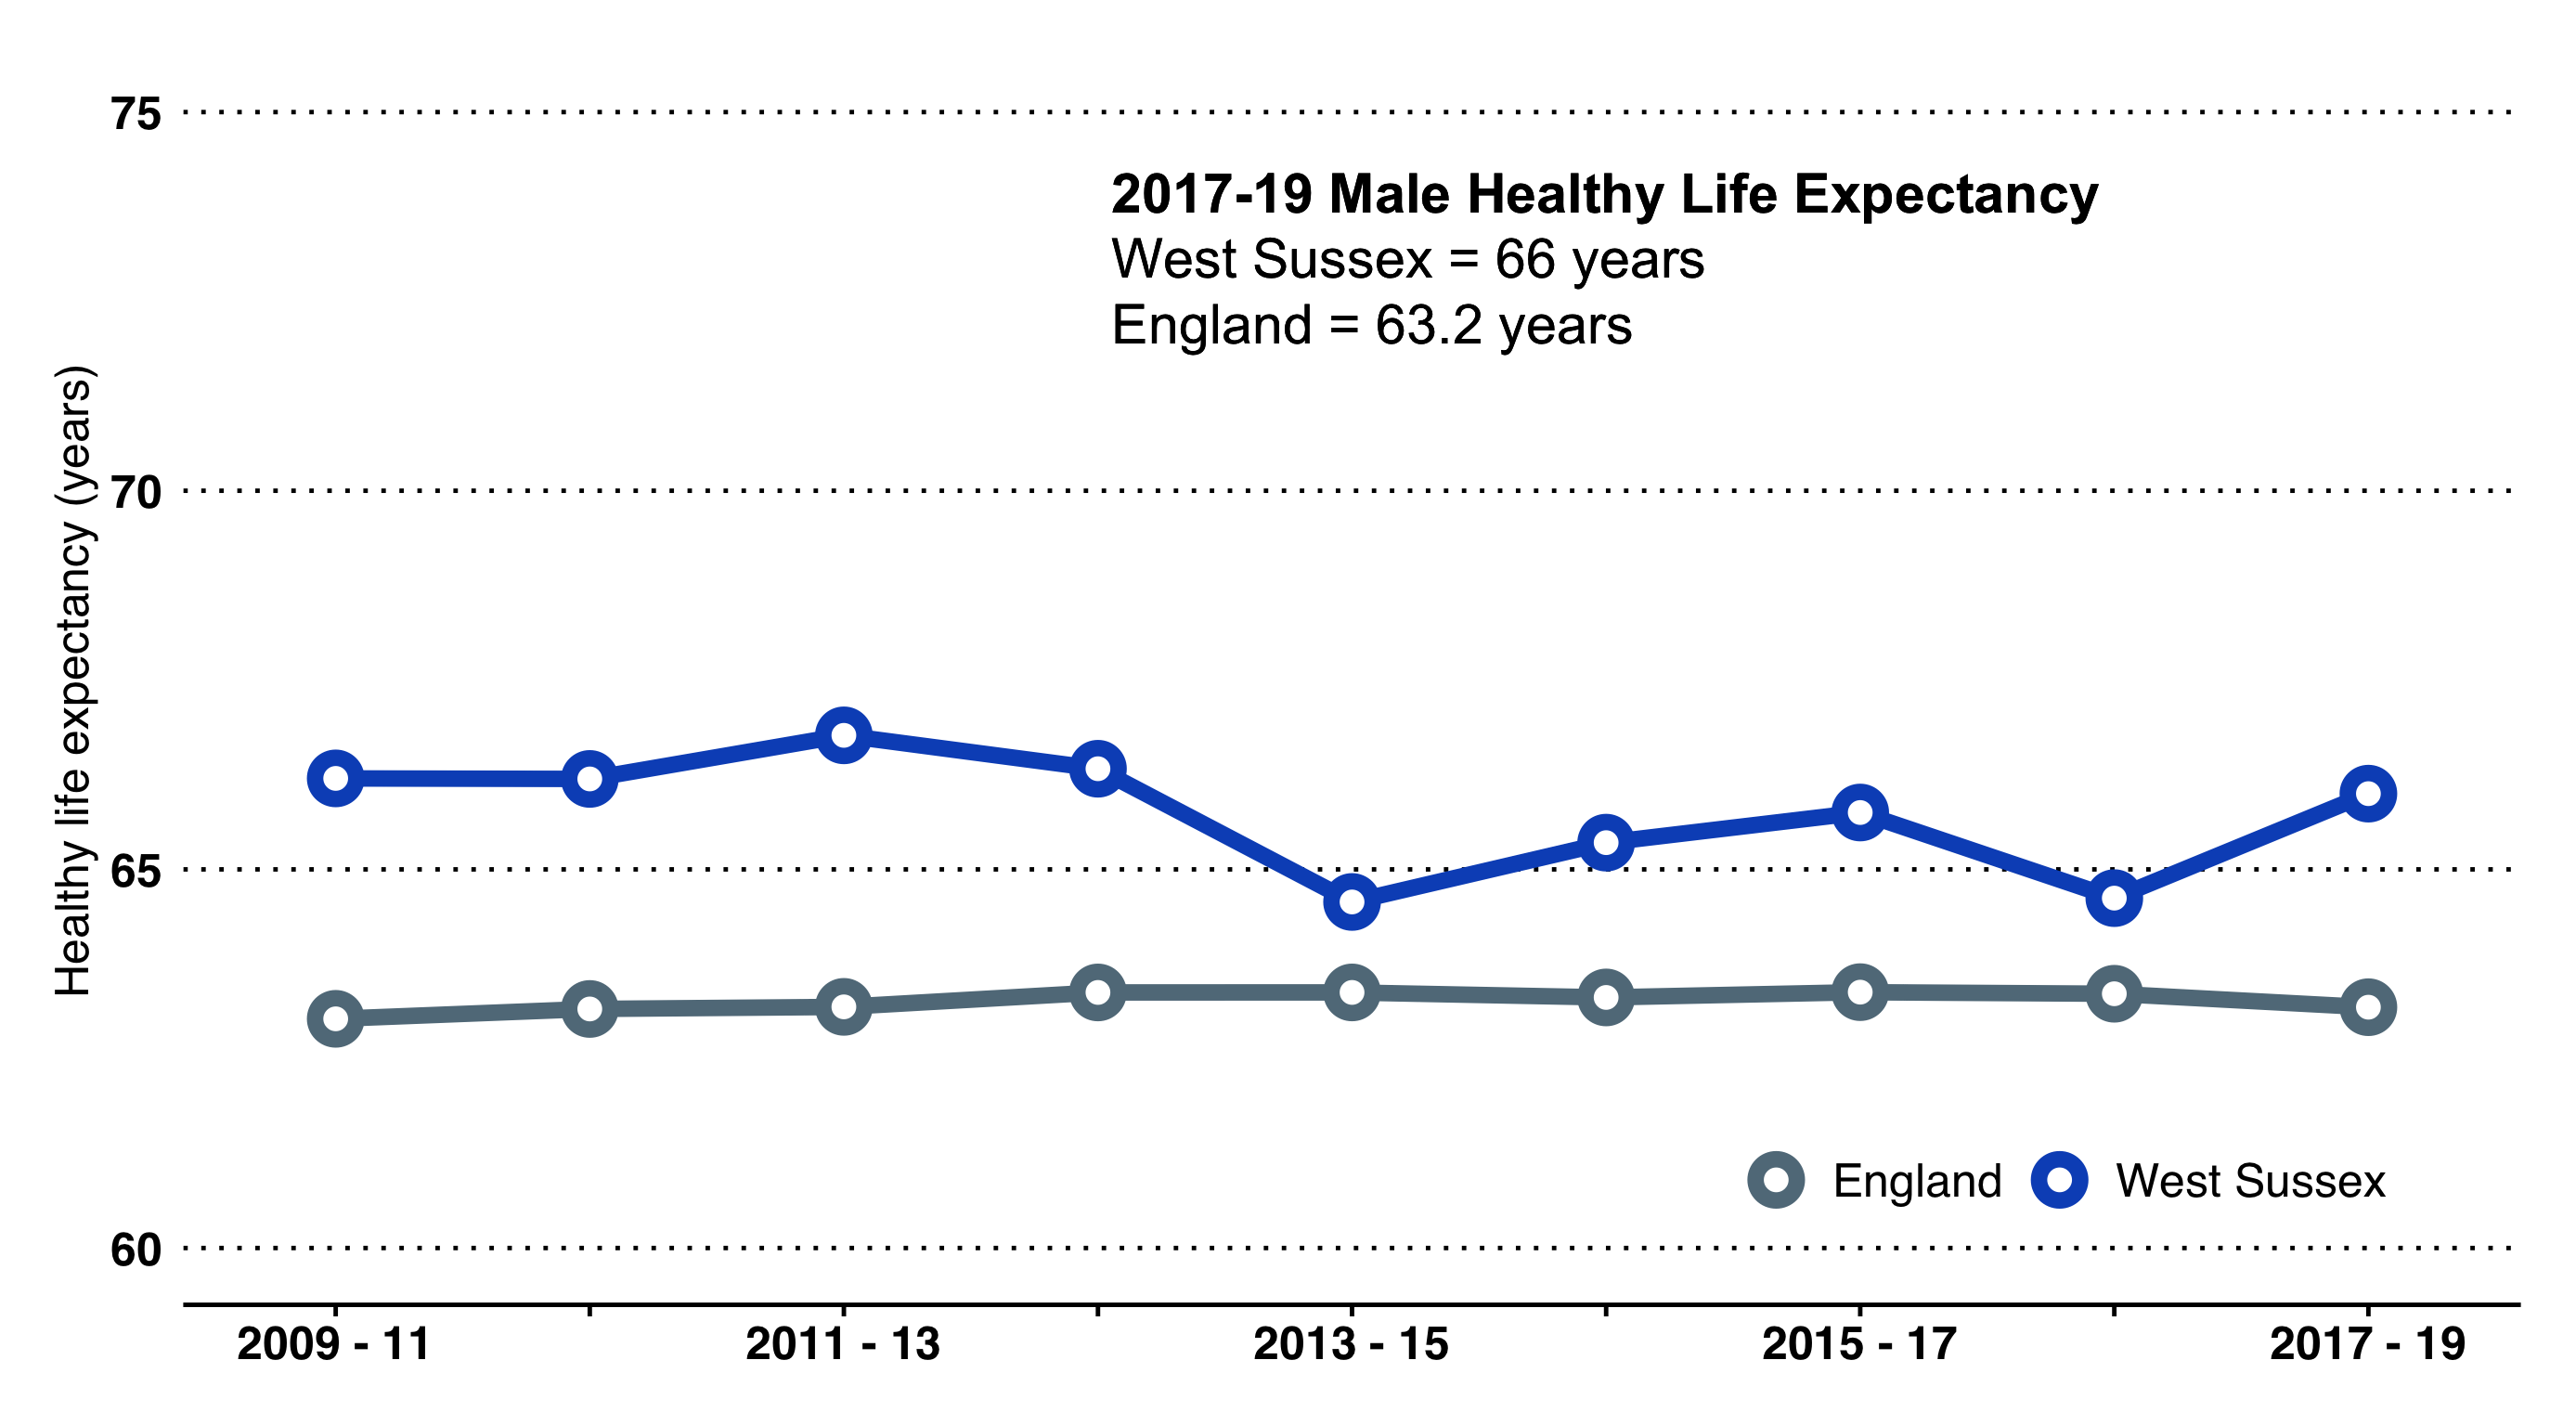
\includegraphics[width=\linewidth]{images/male_HLE.png}
    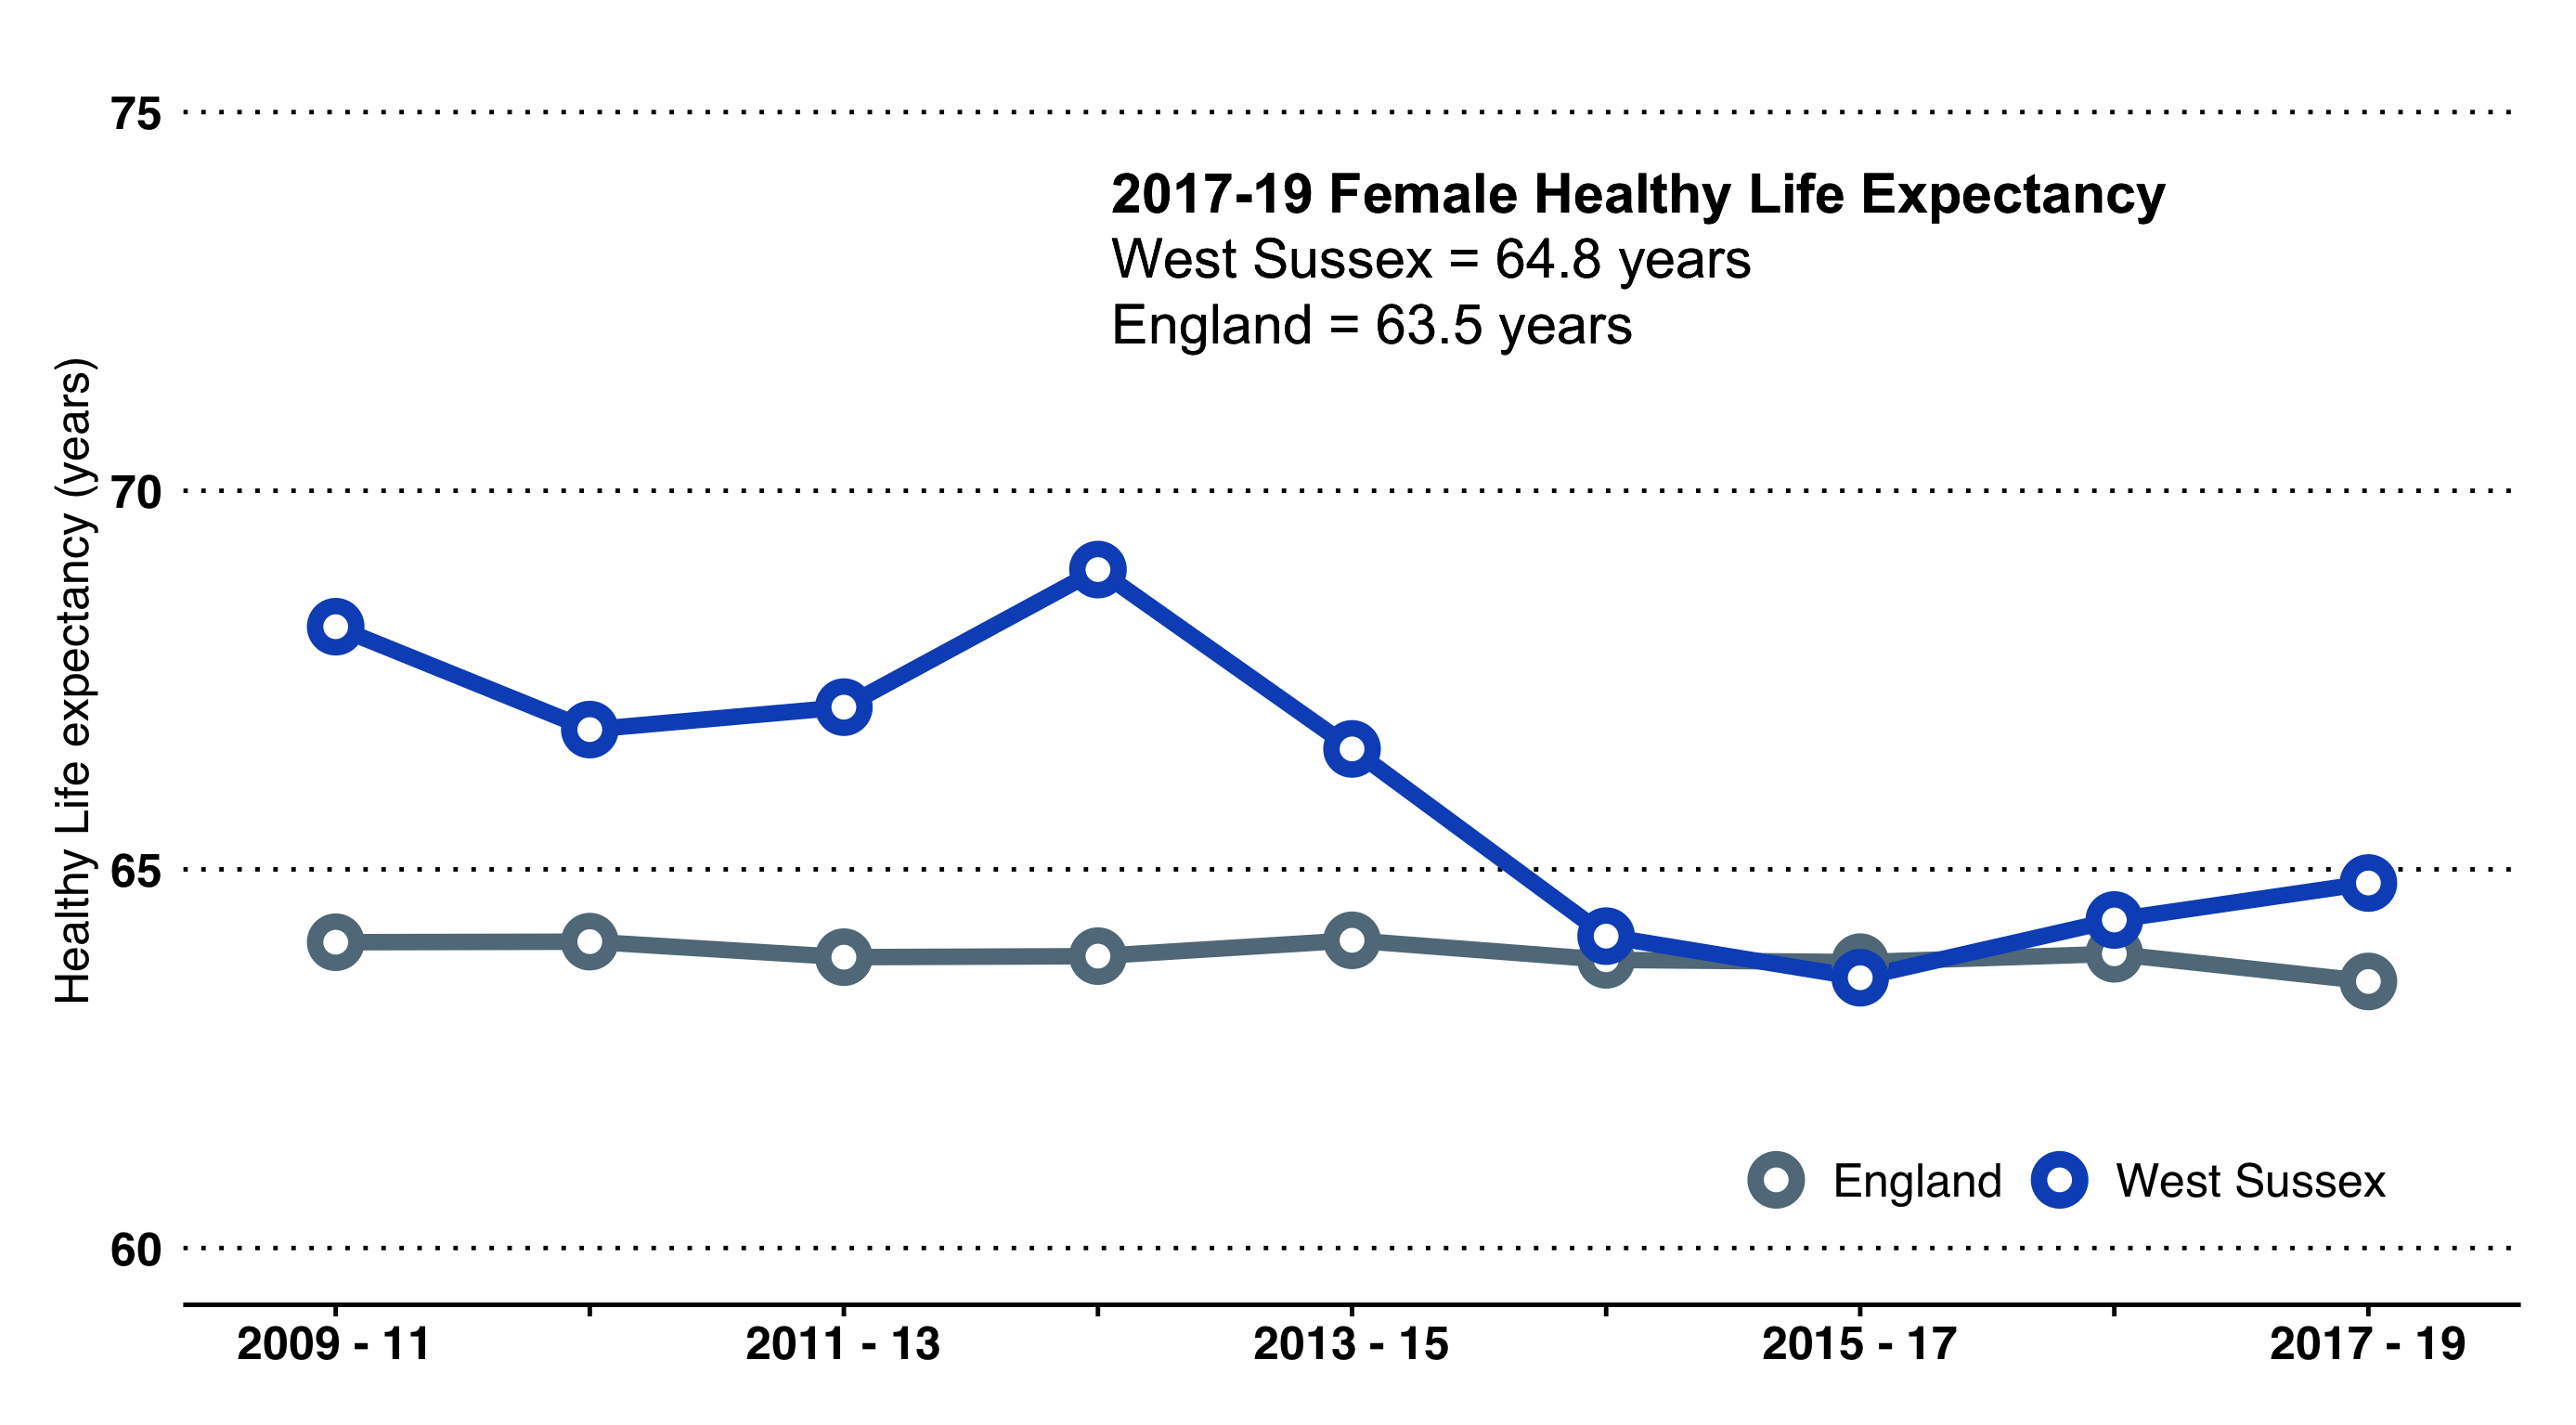
\includegraphics[width=\linewidth]{images/female_HLE.png}
	\label{fig:hle_wsx}
\end{figure}

Healthy life expectancies in West Sussex are comparable to England. In 2017-19, the male healthy life expectancy was 66.0 years and the female healthy life expectancy 64.8 years.

\paragraph{Female Life Expectancy - Changes between 2011-13 and 2017-19} Female healthy life expectancy has fallen considerably in recent years. In 2011-2013, West Sussex ranked 2nd amongst CIPFA comparators but by 2016-18 it had fallen to the second lowest amongst comparable local authorities. In the period 2017-19, West Sussex ranked 10th among comparable local authorities.

\begin{figure}[htp]
    \caption{Female Healthy Life Expectancy at birth - West Sussex compared to its statistical neighbours in 2009-11 and in 2017-19.}
    \centering
	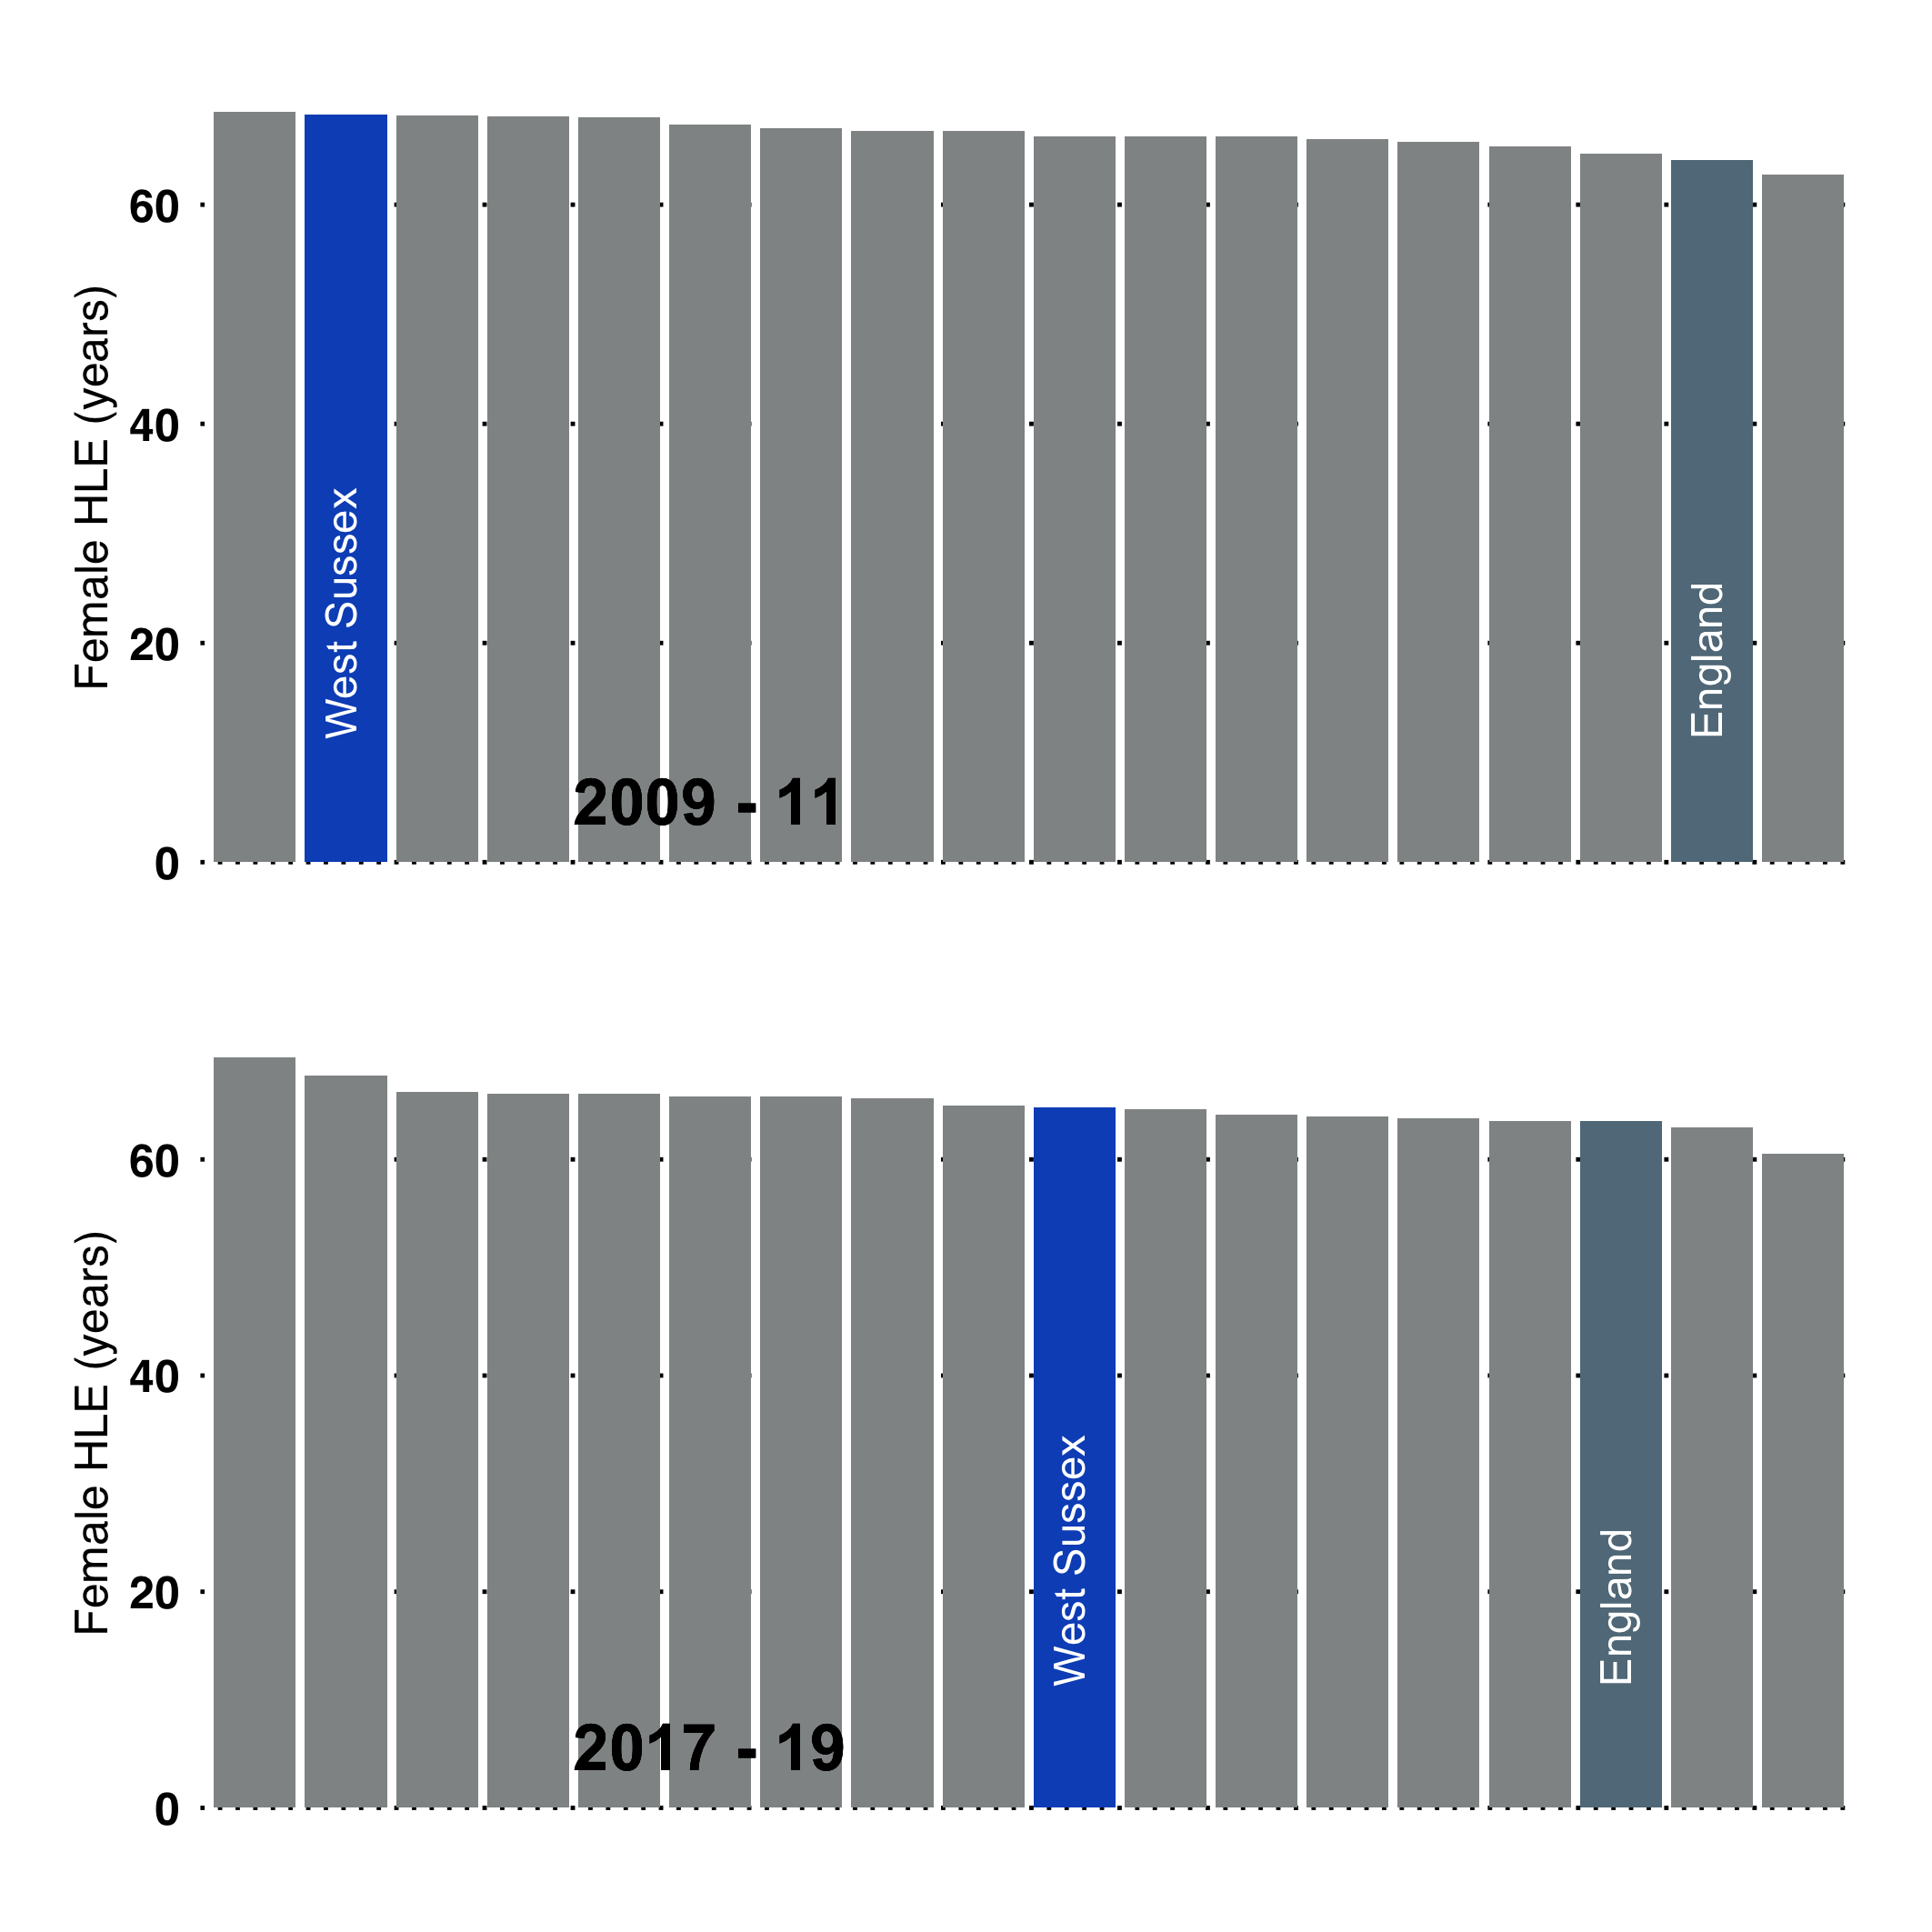
\includegraphics[width=.9\linewidth]{images/hle_cipfa.png}
	\label{fig:hle_cipfa}
\end{figure}

% \subsubsection{A Health Improvement Challenge} Improvements in health can secure considerable benefits.

\begin{tcolorbox}[width=\linewidth, title={A Health Improvement Challenge}, colback={boxcolour}]
As an example, NHS Choices details the benefits of regular activity. For adults aged over 18 years, 150 minutes of moderate activity or 75 minutes intense activity per week is recommended. Ideal moderate activity is brisk walking and cycling, which could be incorporated into active travel.

It is estimated that people who do regular physical activity have up to a:

\begin{itemize}[noitemsep]
    \item 35\% lower risk of coronary heart disease and stroke
    \item 50\% lower risk of type 2 diabetes
    \item 50\% lower risk of colon cancer
    \item 20\% lower risk of breast cancer
    \item 30\% lower risk of early death
    \item 83\% lower risk of osteoarthritis
    \item 68\% lower risk of hip fracture
    \item 30\% lower risk of falls (among older adults)
    \item 30\% lower risk of depression
    \item 30\% lower risk of dementia
\end{itemize}

For West Sussex, if all adults were physically active, this would translate to:

\begin{itemize}[noitemsep]
    \item 10,000 fewer people on coronary heart disease GP register
    \item 23,000 fewer people on diabetes GP register
    \item 20,000 fewer people on depression GP register
    \item 2,500 fewer people on dementia GP register
    \item 175 fewer cases of breast cancer per year
    \item 210 fewer cases of colon cancer per year
    \item 845 fewer emergency admissions for hip fracture in those aged 65 and over
\end{itemize}
\end{tcolorbox}

\subsection{Years of Potential Life Lost - West Sussex Primary Care Networks}
Years of Potential Life Lost (YPLL) is a measure of premature mortality.

If the average life expectancy in an area is 80 years and a death occurs at 50 we can describe the 30 year difference as "potential life years" lost to the population. By summing all the life years lost of people who have died prematurely we can calculate a summary for an area/group. People who die at a younger age contribute greater number of years; for example, a young person who dies at 20 in a car accident will have 60 years of life lost, whereas someone who dies at 72 would have 8 years of life lost. In using this measure, we look at the overall level of premature mortality (as a rate per 10,000 population) and at the cause of premature mortality so that we can identify the key causes of premature mortality.

For comparison with the previous JSNA summary, we  have again looked at deaths under the age of 75 by Primary Care Networks in West Sussex. We have summed the total years of life lost for deaths between 2017 and 2021 (5 years of data), calculated as a rate per PCN population aged under 75 years. (Figure~\ref{fig:ypll})

\begin{figure}[htp]
    \caption{Years of Potential Life Lost Rate per 10,000 Population (U75) Pooled Data of Deaths Registered Between 2017 and 2021.}
    \centering
	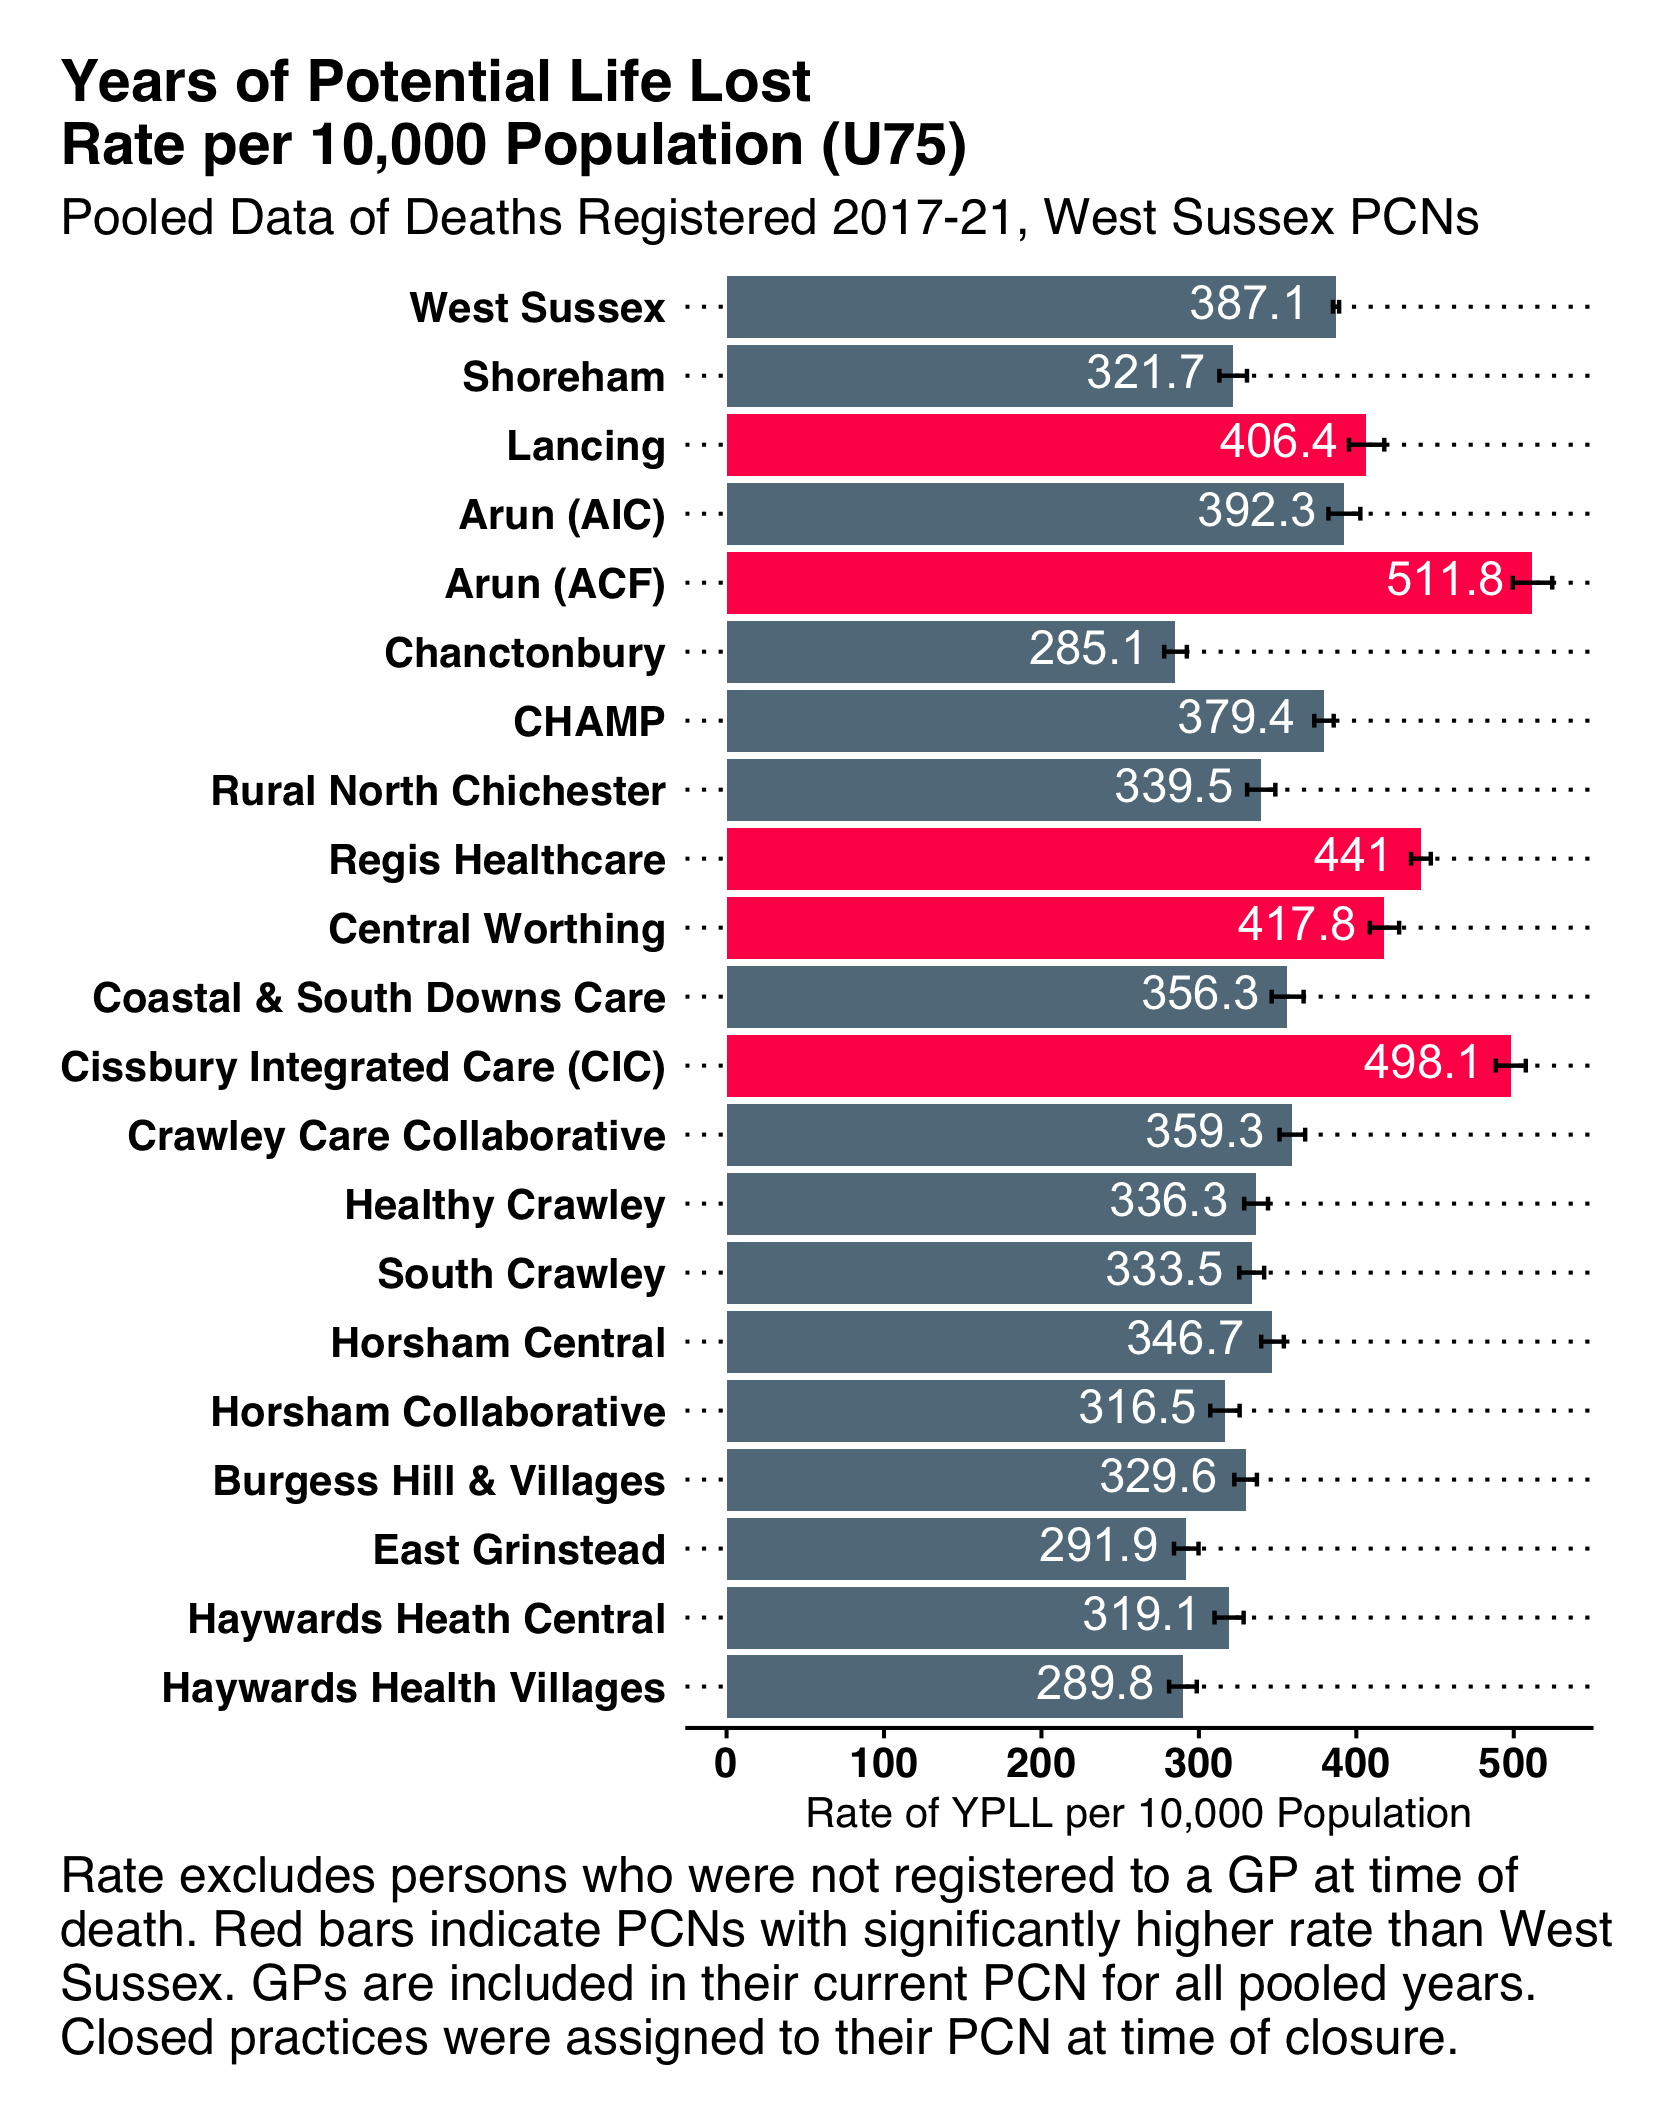
\includegraphics[width=\linewidth]{images/ypll_by_pcn.png}
	\label{fig:ypll}
\end{figure}

% https://www.healthknowledge.org.uk/public-health-textbook/research-methods/1a-epidemiology/years-lost-life

Five PCNs have rates significantly higher compared with the West Sussex overall rate. These are Lancing, Arun (Neighbourhood 1), Regis (Neighbourhood I - Central Regis) and Cissbury. 

The top 5 causes of years of potential life lost are common across all the PCNs: cancer, diseases of the circulatory, respiratory and digestive systems, and external causes (such as accidents).

\subsection{Employment and Unemployment}
\paragraph{Economic Inactivity}
In West Sussex 92,900 people aged 16-64 years are estimated to be economically inactive (April 2020 to March 2021). Of these, over 68,500 are not seeking a job; with 16,000 people with long term sickness, 14,900 looking after the home or family, and 15,700 retired.

\paragraph{Long-term claimants of Jobseeker's Allowance}

The rate per 1,000 16-64 year-olds claiming Jobseeker' Allowance long-term (i.e. for more than 12 months) has improved in West Sussex in recent years, decreasing from 4.9 per 1,000 in 2012 to 1.8 per 1,000 in 2018 (a decrease of 1,455 people in this time period). The West Sussex rate is in line with CIPFA neighbours and below England (3.8 per 1,000 in 2018).

\begin{figure}[htp]
    \caption{Long-term claimants of Jobseeker' Allowance by West Sussex Local Authorities, 2020}\label{fig:longterm_jsa}
    \centering
	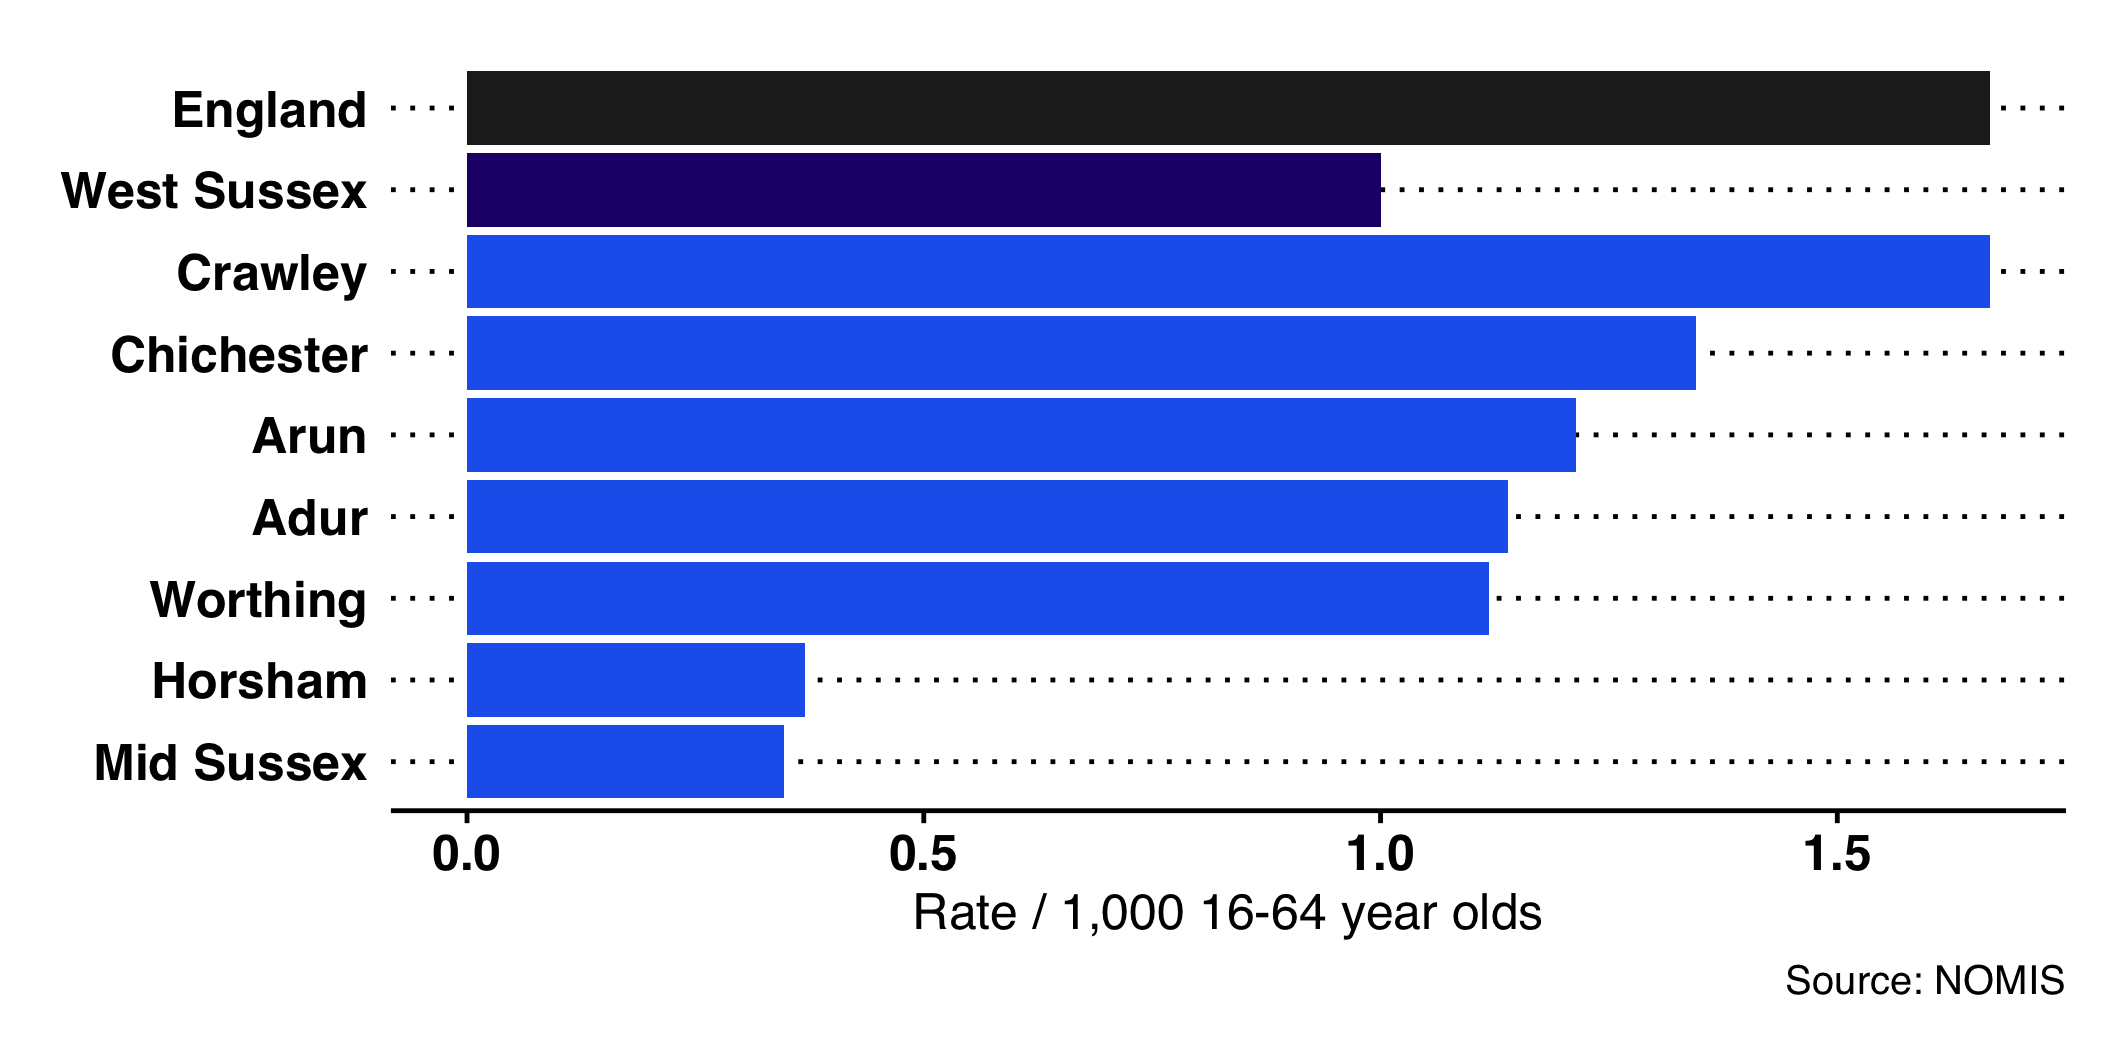
\includegraphics[width=.9\linewidth]{images/longterm_jsa_claimants_wsx.png}
\end{figure}

\paragraph{Out-Of-Work Benefits} In West Sussex, there are a similar proportion of claimants to the South East region as a whole (3.2\% compared to 3.3\%), this was approximately 16,300 people in March 2022. The number of claimants was higher during the first Covid lockdown (at a peak of 27,500 in May 2020) but has fallen since.\footnote{Under Universal Credit a broader span of claimants are required to look for work than under Jobseeker's Allowance. As Universal Credit Full Service is rolled out in particular areas, the number of people recorded as being on the Claimant Count is therefore likely to rise.}

The Claimant Count is the number of people claiming benefit principally for the reason of being unemployed. This is measured by combining the number of people claiming Jobseeker's Allowance (JSA) and National Insurance credits with the number of people receiving Universal Credit principally for the reason of being unemployed. Claimants declare that they are out of work, capable of, available for and actively seeking work during the week in which the claim is made. Note that the Claimant Count is currently designated as an experimental statistic.

\paragraph{Employment Rate Gap of Vulnerable Groups}

The employment rate gap looks at the difference in the percentage of people who are part of a vulnerable group who are employed, compared to the percentage of all respondents in the Labour Force Survey classed as employed (aged 16-64)\footnote{PHOF references B08a, B08b and B08c.}.

In 2019/20, the employment rate gap for people with learning disability was significantly greater in West Sussex (78.6\%) compared to the overall rate across England (70.6\%).

In 2019/20, for both people with a long-term health condition, and people in contact with secondary mental health services, the employment rate gaps were similar in West Sussex compared with the overall rates across England.

The rate gap for people with a long term health condition has improved, decreasing from 14.3\% in 2018/19 to 9.9\% in 2019/20, similar to the England rate (67.2\%)\footnote{PHOF references B08a, B08b and B08c.}.

The rate gap for people in contact with secondary mental health services has remained at a similar level, decreasing from 69.1\% in 2018/19 to 68.7\% in 2019/20, similar to the England rate (67.2\%).

% This figure isn't great (as at 16/6), text renders too small on the labels. Current idea is to fill the bars with the text for the two longer bars? I'm still not that great at annotating plots outside the data ranges...

\begin{figure}[htp]
    \caption[Gaps in employment rate, West Sussex 2019/20.]{Gaps in employment rate for people with long term health conditions, people in contact with secondary mental health services, and people with learning disabilities. West Sussex, 2019/20.}\label{fig:emp_gaps}
    \centering
	
\includegraphics[width=.9\linewidth]{images/employment_gaps.png}
\end{figure}

\paragraph{Employment Deprived} As part of the Index of Deprivation 2019, the employment domain provides information on the proportion of the working age population in an area that are involuntarily excluded from the labour market. These are people who would like to work but are unable to, including those unemployed, ill, disabled or who have caring responsibilities.

\begin{table}[hbt]
    \caption{The proportion of working age population in West Sussex local authorities that are involuntarily excluded from the labour market. The England rate is 9.9\%.}
    \centering
    \begin{tabular}{lrr}
    \toprule
    \ & Number & Percentage \\
    \midrule
    Adur & 3,100 & 8.9 \\
    Arun & 7,000 & 9.0 \\
    Chichester & 3,900 & 6.4\\
    Crawley & 5,200 & 7.7\\
    Horsham & 3,800 & 5.1\\
    Mid Sussex & 3,700 & 4.6\\
    Worthing & 5,400 & 9.0\\
    West Sussex & 32,100 & 7.0\\
    \bottomrule
    \end{tabular}
    \label{tab:wa:empdep}
\end{table}

\subsubsection{Health and Social Care Workforce - Primary Care}
\paragraph{Primary Care Staffing} By West Sussex Clinical Commissioning Group (CCG). Data are estimated provided as of March 2022 by NHS Digital.\footnote{Note that direct patient care staff includes therapists, health care assistant, social prescribing link workers etc. FTE = Full Time Equivalent.}
% NB - might have three columns here staff type, FTE, head count
\begin{table}[hbt]
    \caption[Primary Care Staffing in NHS West Sussex CCG, March 2022.]{Primary Care Staffing in NHS West Sussex CCG, March 2022.}
    \centering
    \begin{tabular}{lrr}
    \toprule
    Staff Role & FTE & Headcount \\
    \midrule
    All GPs  & 474 & 647  \\
    Fully qualified GPs \scriptsize{(excludes Registrars)} & 575 & 404 \\
    Qualified permanent GPs \scriptsize{(excludes Registrars and Locums)} & 567 & 400 \\
    Nurses & 340 & 230 \\
    Direct patient care staff & 350 & 233 \\
    Admin / non-clinical staff & 1572 & 1090 \\
    \bottomrule
    \end{tabular}
    \label{tab:wa:primarystaff}
\end{table}

% \todo[inline]{Find where I put the data on GPs aged 55+}

% \begin{table}[hbt]
%     \caption{Percentage of GPs Aged 55 or Over by West Sussex CCGs.}
%     \centering
%     \begin{tabular}{lrrrr}
%     \toprule
%     \ CWS & Craw & HMS & England \\
%     \midrule
%     \% GPs Over 55 & 17.9 & 25.3 & 16.1 & 19.5 \\
%     \bottomrule
%     \end{tabular}
%     \label{tab:wa:primarystaff_o55}
% \end{table}

% Will compare all staff roles in a new version of this chart
% FIGURES Staffing (FTE) per 100,000 Population -> GPs / Nurses / Direct Care Staff / Admin and non-clinical\footnote{CWS = Coastal West Sussex CCG, Craw = Crawley CCG, HMS = Horsham and Mid Sussex CCG}

\subsection{Health and Social Care Workforce - Social Care / Care Benefits}
Data from Skills for Care\footnote{\url{https://www.skillsforcare.org.uk/adult-social-care-workforce-data/Workforce-intelligence/Home.aspx}}:
\begin{itemize}[noitemsep]
    \item Adult Social Care Workforce Data Set (ASC-WDS) (as at February 2022)
    \item Independent sector employees as at September 2021
\end{itemize}

\begin{figure}[h]
    \centering
    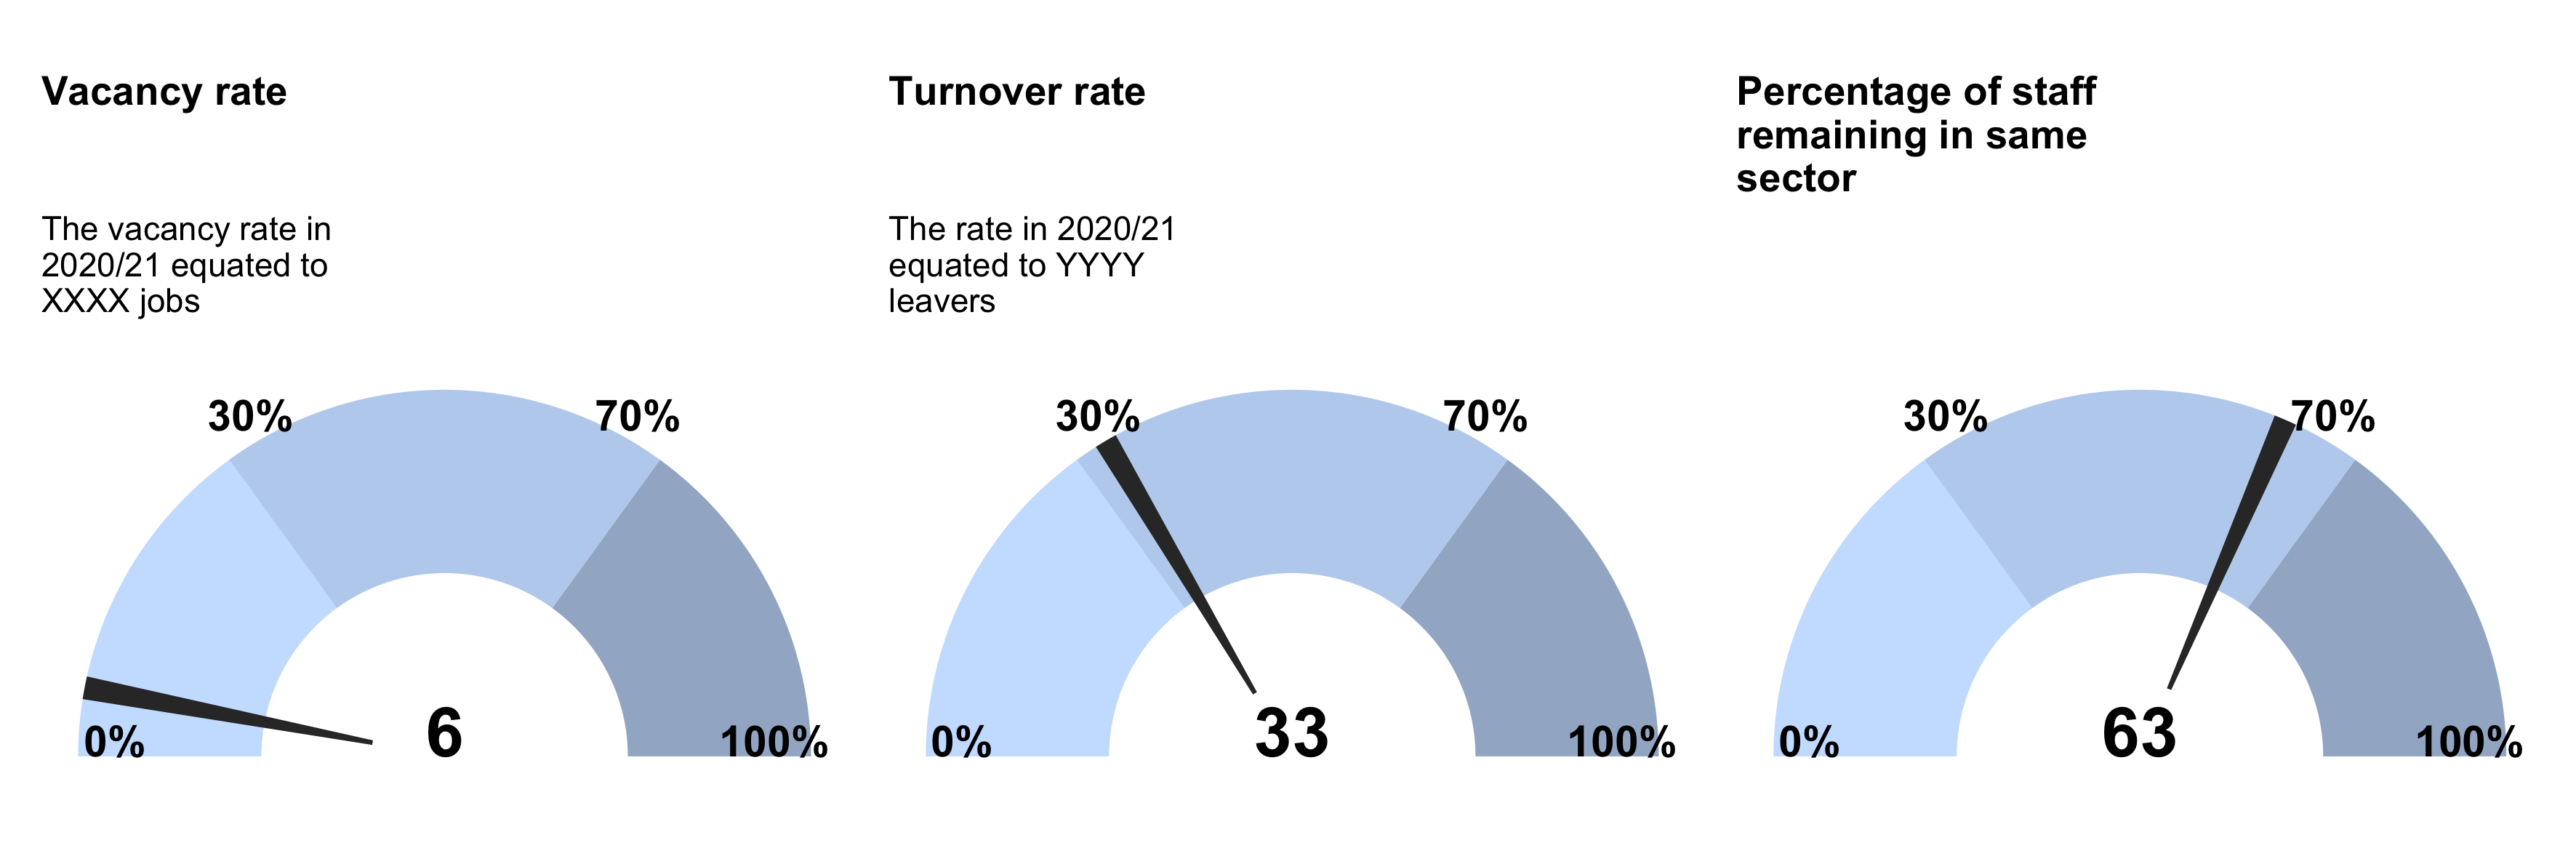
\includegraphics[width=\linewidth]{images/workforce_dial_chart.png}
\end{figure}

\begin{itemize}[noitemsep]
    \item Vacancy rate - The vacancy rate in 2020/21 equated to 1,300 jobs - 6\%
    \item Turnover Rate - The rate in 2020/21 equated to 6,800 leavers - 33\%
    \item Percentage of staff remaining in same sector - 66\%
\end{itemize} 

\begin{figure}[h]
    \caption{Estimated Number of Social Care Staff (all sectors)}\label{fig:sc-workforce}
    \centering
    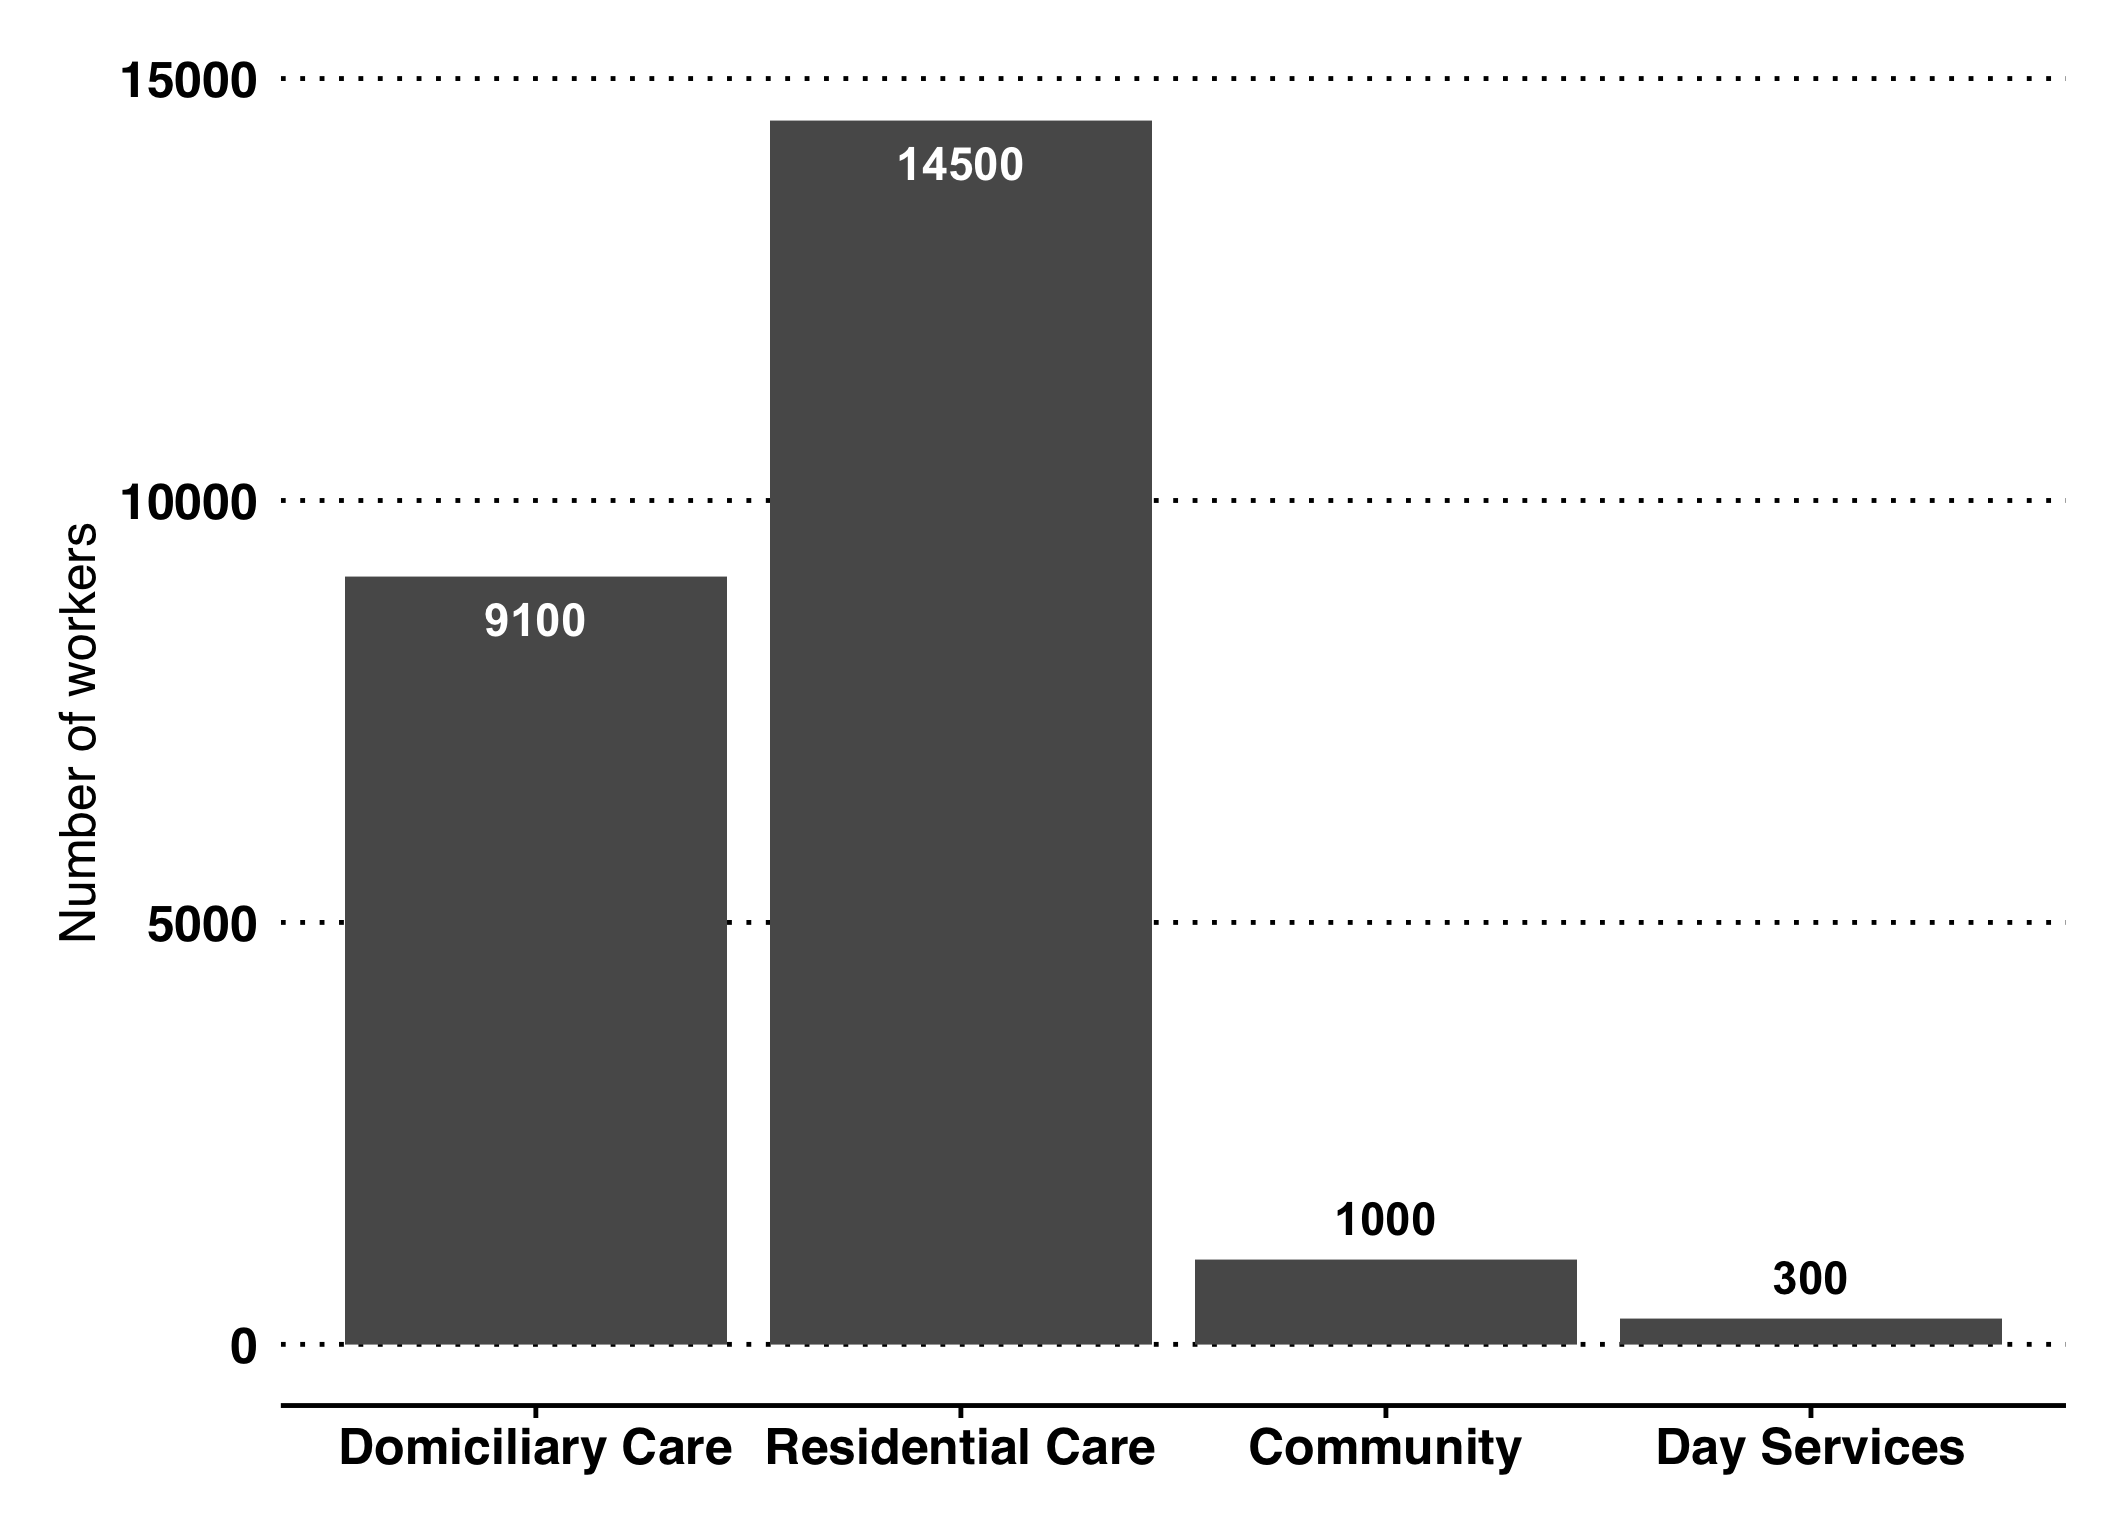
\includegraphics[width = \linewidth]{images/03-sc-workforce.png}
\end{figure}

\begin{itemize}[noitemsep]
    \item 27\% of workers are over 55
    \item Average Age = 44
    \item 82\% female
    \item 23\% of workers on zero hours contracts
    \item On average 8.8 days of sickness per year
\end{itemize}
   
\paragraph{Attendance Allowance - November 2021 (Rounded to nearest 10)} Attendance Allowance (AA) is non-means tested contribution towards additional costs incurred by people who have a disability and are aged 65 years or over. To qualify, people need to require help with personal care for at least 6 months. Payments are made at two rates: the lower rate (for people who need frequent help or constant supervision during the day, or supervision at night) and the higher rate (for people who need help or supervision throughout both day and night, or who are terminally ill).

\begin{table}[hbt]
    \caption{Attendance Allowance - November 2021}
    \centering
    \begin{tabular}{llll}
    \toprule
    \ & Total (People) & On Lower Rate & On Higher Rate \\
    \midrule
    Adur & 1,790 & 740 & 1,050 \\
    Arun & 5,370 & 2,090 & 3,290 \\
    Chichester & 3,310 & 1,220 & 2,100 \\
    Crawley & 1,840 & 800 & 1,040 \\
    Horsham & 3,200 & 1,310 & 1,890 \\
    Mid Sussex & 2,920 & 1,250 & 1,680 \\
    Worthing & 2,930 & 1,190 & 1,740 \\
    West Sussex & 21,360 & 8,590 & 12,780 \\
    \bottomrule
    \end{tabular}
    \label{tab:wa:att_all}
\end{table}



\paragraph{Carers Allowance - November 2021 (Rounded to nearest 10)} This is paid to people (aged 16 or over) who look after a severely disabled person for at least 35 hours a week and who are not employed (i.e. not earning more than £95 per week after certain deductions) and not in full-time education. The disabled person must be receiving specific benefits relating to their disability. The mean amount paid is £65.90 per week.

% Note: these figures are lot higher than the last JSNA summary (May 2019) so could demonstrate impact of the pandemic on claimants of carers allowance.
\begin{table}[hbt]
    \caption{Carers Allowance - November 2021.}
    \centering
    \begin{tabular}{ll}
    \toprule
    \ & Total \\
    \midrule
    Adur & 1,120 \\
    Arun & 2,720 \\
    Chichester & 1,580 \\
    Crawley & 1,820 \\
    Horsham & 1,530 \\
    Mid Sussex & 1,480 \\
    Worthing & 1,710 \\
    Total & 11,950 \\
    \bottomrule
    \end{tabular}
    \label{tab:wa:car_all}
\end{table}

\begin{figure}[h]
    \caption{Carers Allowance - November 2021 Age and Gender of Claimants}\label{fig:carer-claims-age-gender}
    \centering
    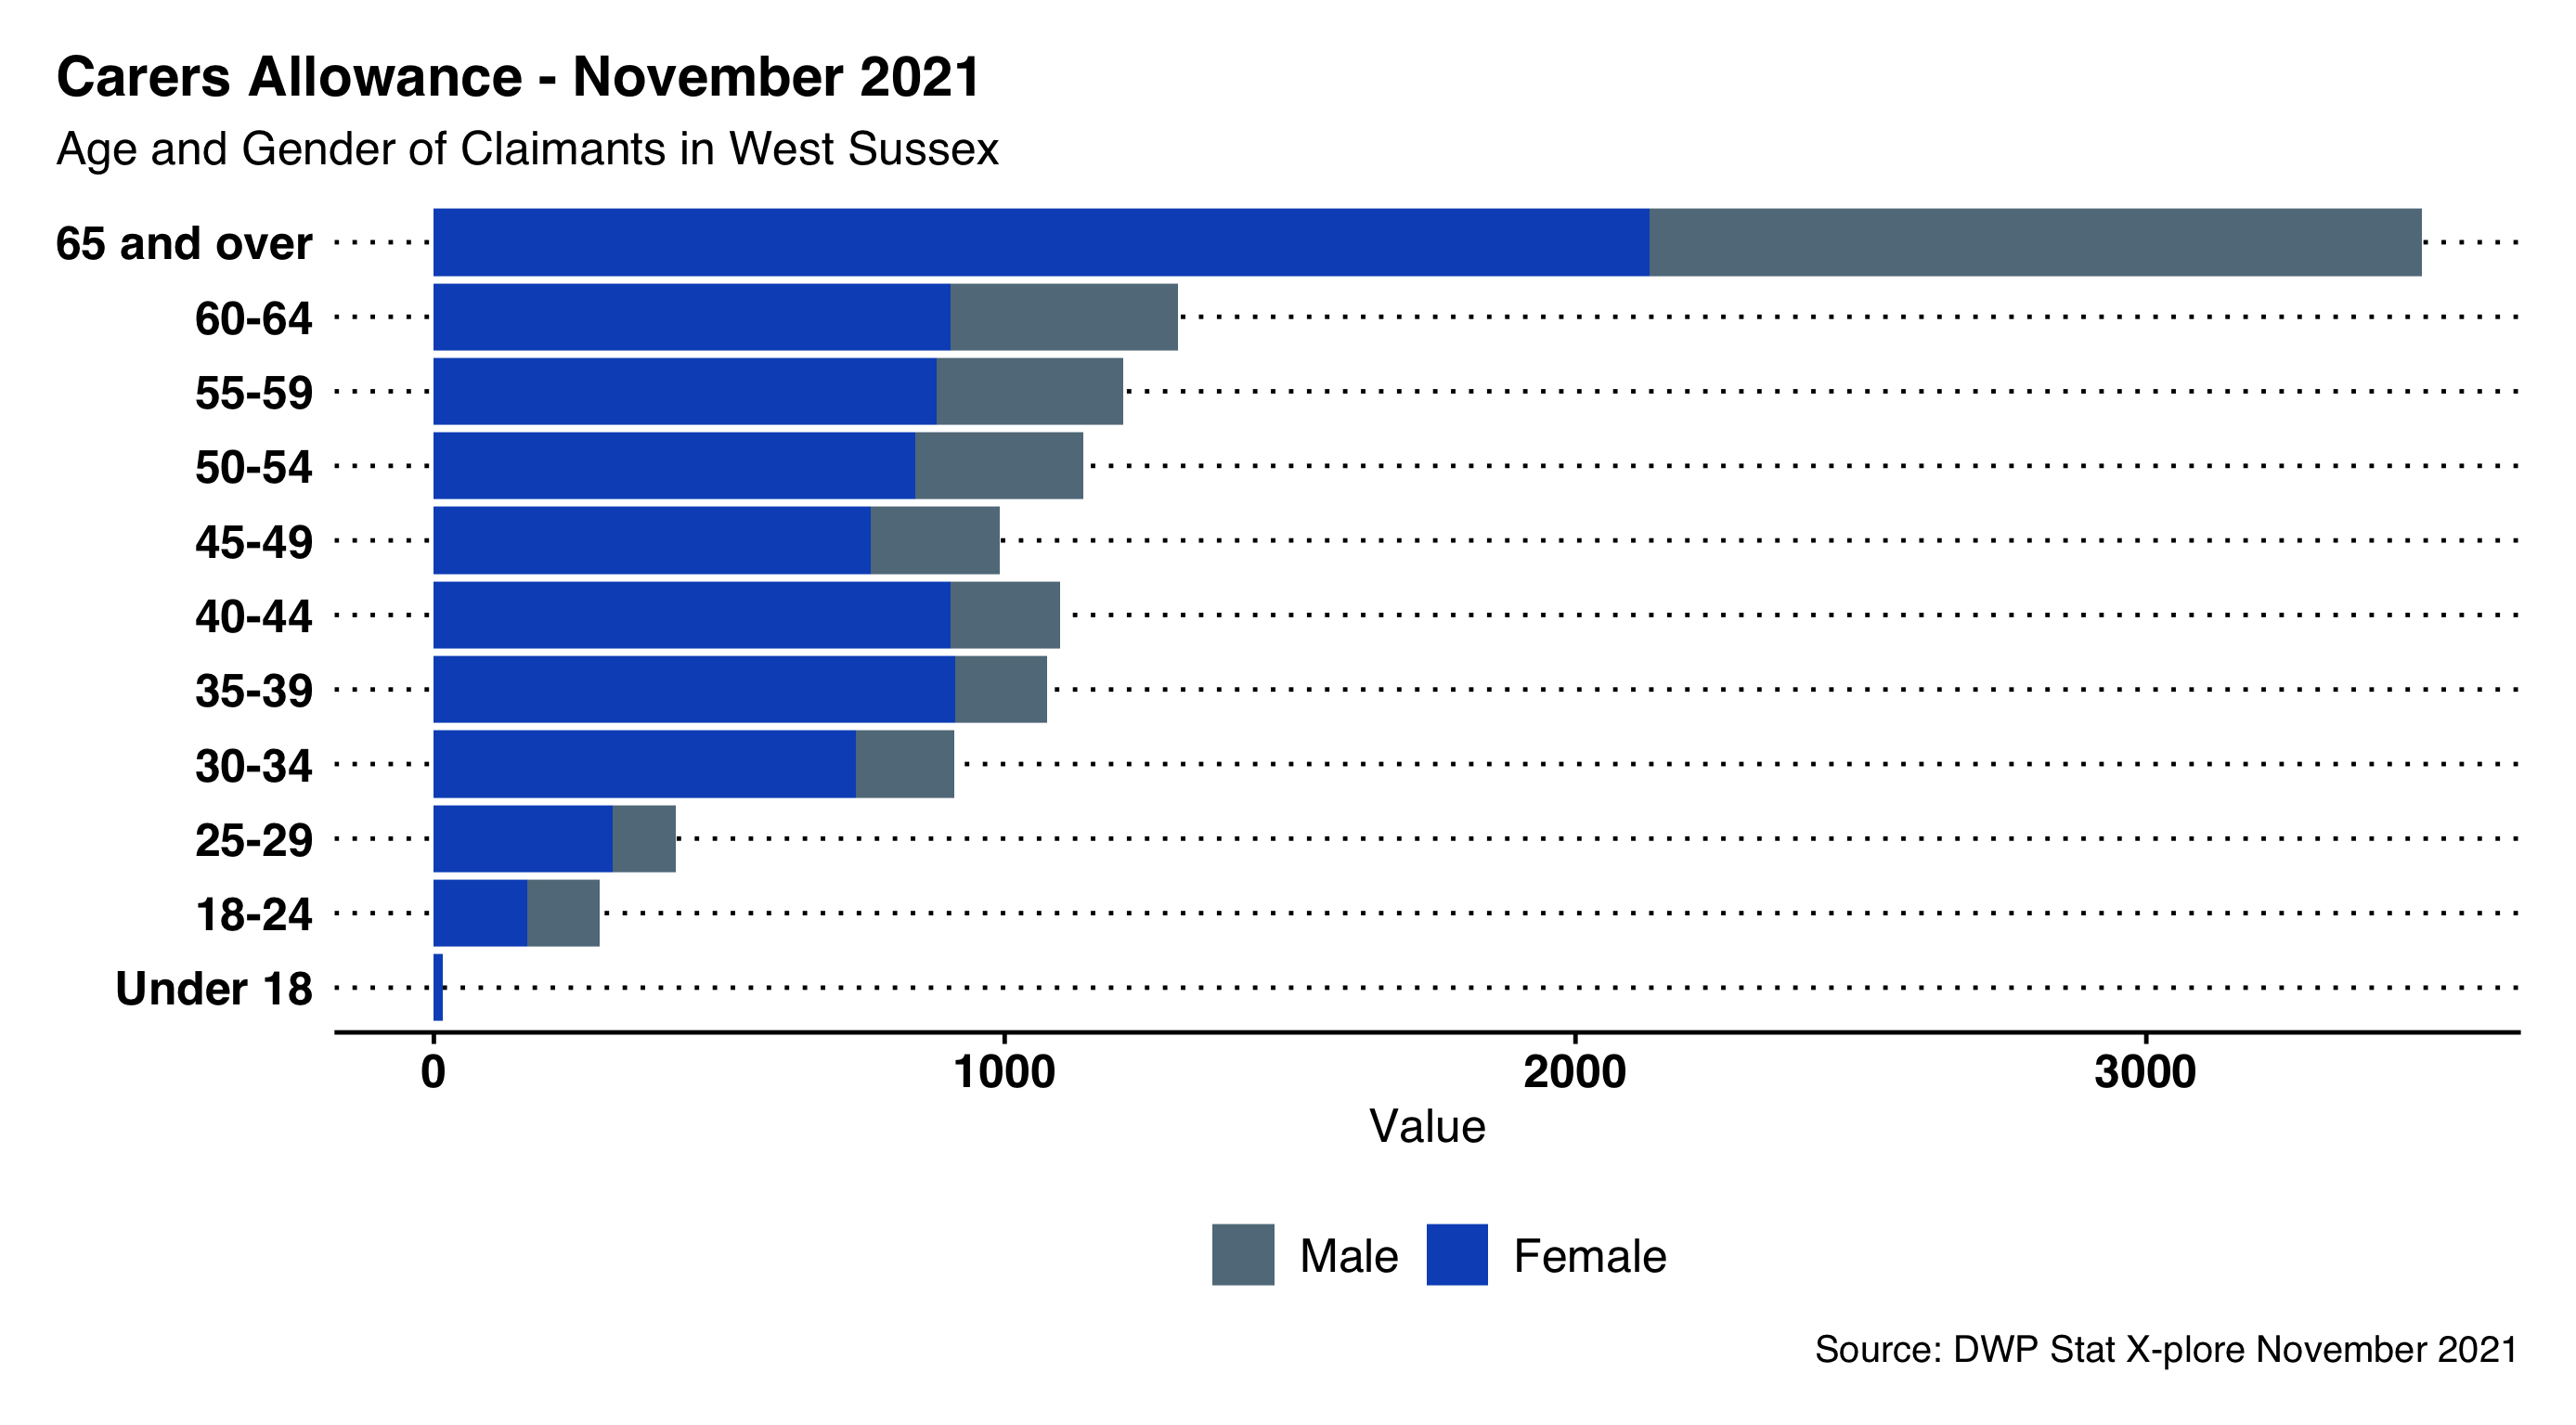
\includegraphics[width=\linewidth]{images/carers_allowance_recipients.png}
\end{figure}


\subsection{Unpaid Care}
\paragraph{Unpaid Care}There are an estimated 90,405 unpaid carers of all ages in West Sussex, representing 10.4\% of the total population (similar to the England proportion).

Women tend to take on more caring responsibilities than men, with an estimated 52,652 female carers compared to 37,704 male carers.

\begin{figure}[h]
    \caption{Estimated number of unpaid carers in West Sussex, by age and sex. 2011 Census estimates applied to 2020 mid-year population estimates.}\label{fig:unpaid-carers-sex-age}
    \centering
    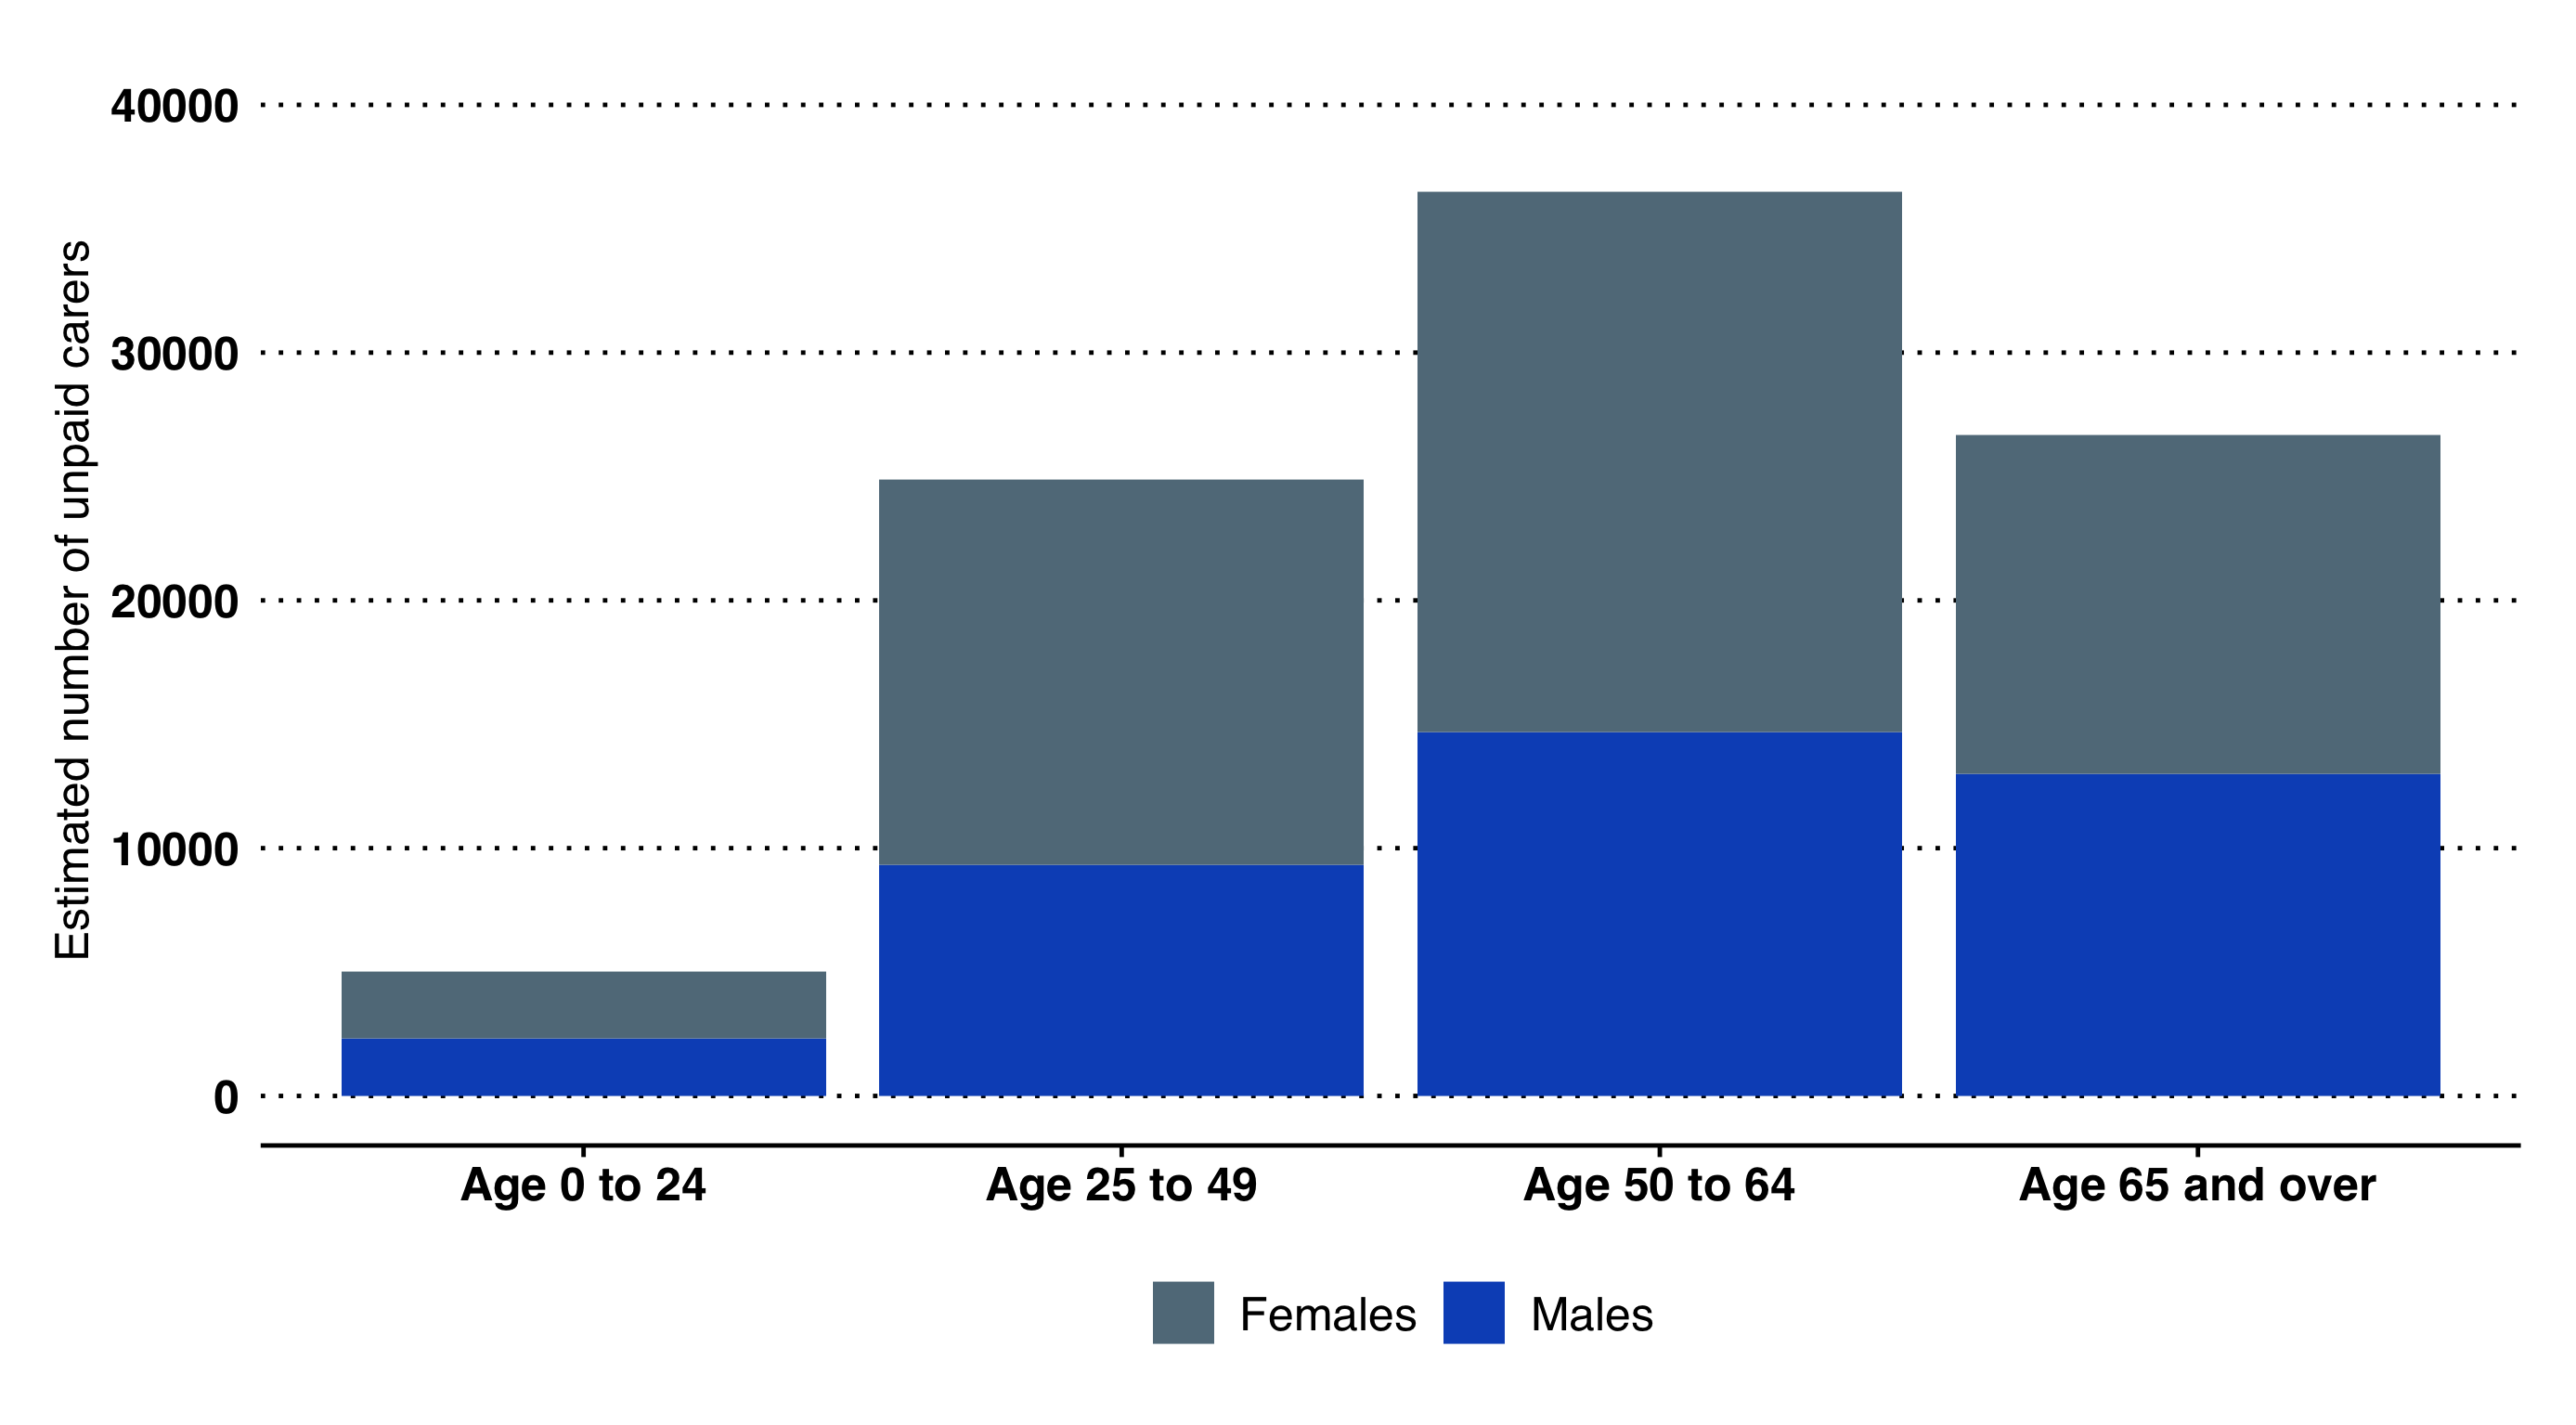
\includegraphics[width=\linewidth]{images/wsx_unpaid_carers_by_age.png}
\end{figure}

Those of working age (ages 25-64) account for 68\% of unpaid care, whilst over- 65s account for 29\%.

Arun has the greatest number of unpaid carers of all ages, at 17,753, followed by Mid Sussex (15,144) and Mid-Sussex (15,042). Adur has the fewest number of unpaid carers, at 7,277.

\paragraph{50 or more unpaid care hours per week}Of the total number of carers in West Sussex, approximately a fifth are estimated to do 50 or more hours of unpaid care a week (slightly below the England proportion). This burden of care again falls more heavily on female carers (over 11,000 female carers, compared to nearly 7,500 male carers, do >50 hours per week).

Over 65s make up the majority of carers doing >50 hours per week; 37.5\% of female carers and 51.6\% of male carers doing >50 hours are in this age-group.

Adur has the greatest proportion of unpaid carers doing >50 hours per week, followed by Arun.

\paragraph{How do we estimate the numbers of unpaid carers?} The Carers Trust defines a carer as anyone who cares, unpaid, for a friend or family member who due to illness, disability, mental health problems or an addiction cannot cope without their support. The current number of unpaid carers in West Sussex can be estimated by applying the percentage of unpaid carers in the population, as recorded in the most recent census (2011), to the latest population estimates (2020).

\newpage

\begin{figure}
    \caption{Estimated number of unpaid carers in West Sussex. 2011 Census estimates applied to 2020 mid-year population estimates.}
    \label{figure:unpaidcarers:dabs}
    \centering
    \begin{subfigure}[b]{0.99\linewidth}
        \centering
        \caption{Female carers by West Sussex Local Authorities.}\label{fig:unpaidcarers:dabs:female}
        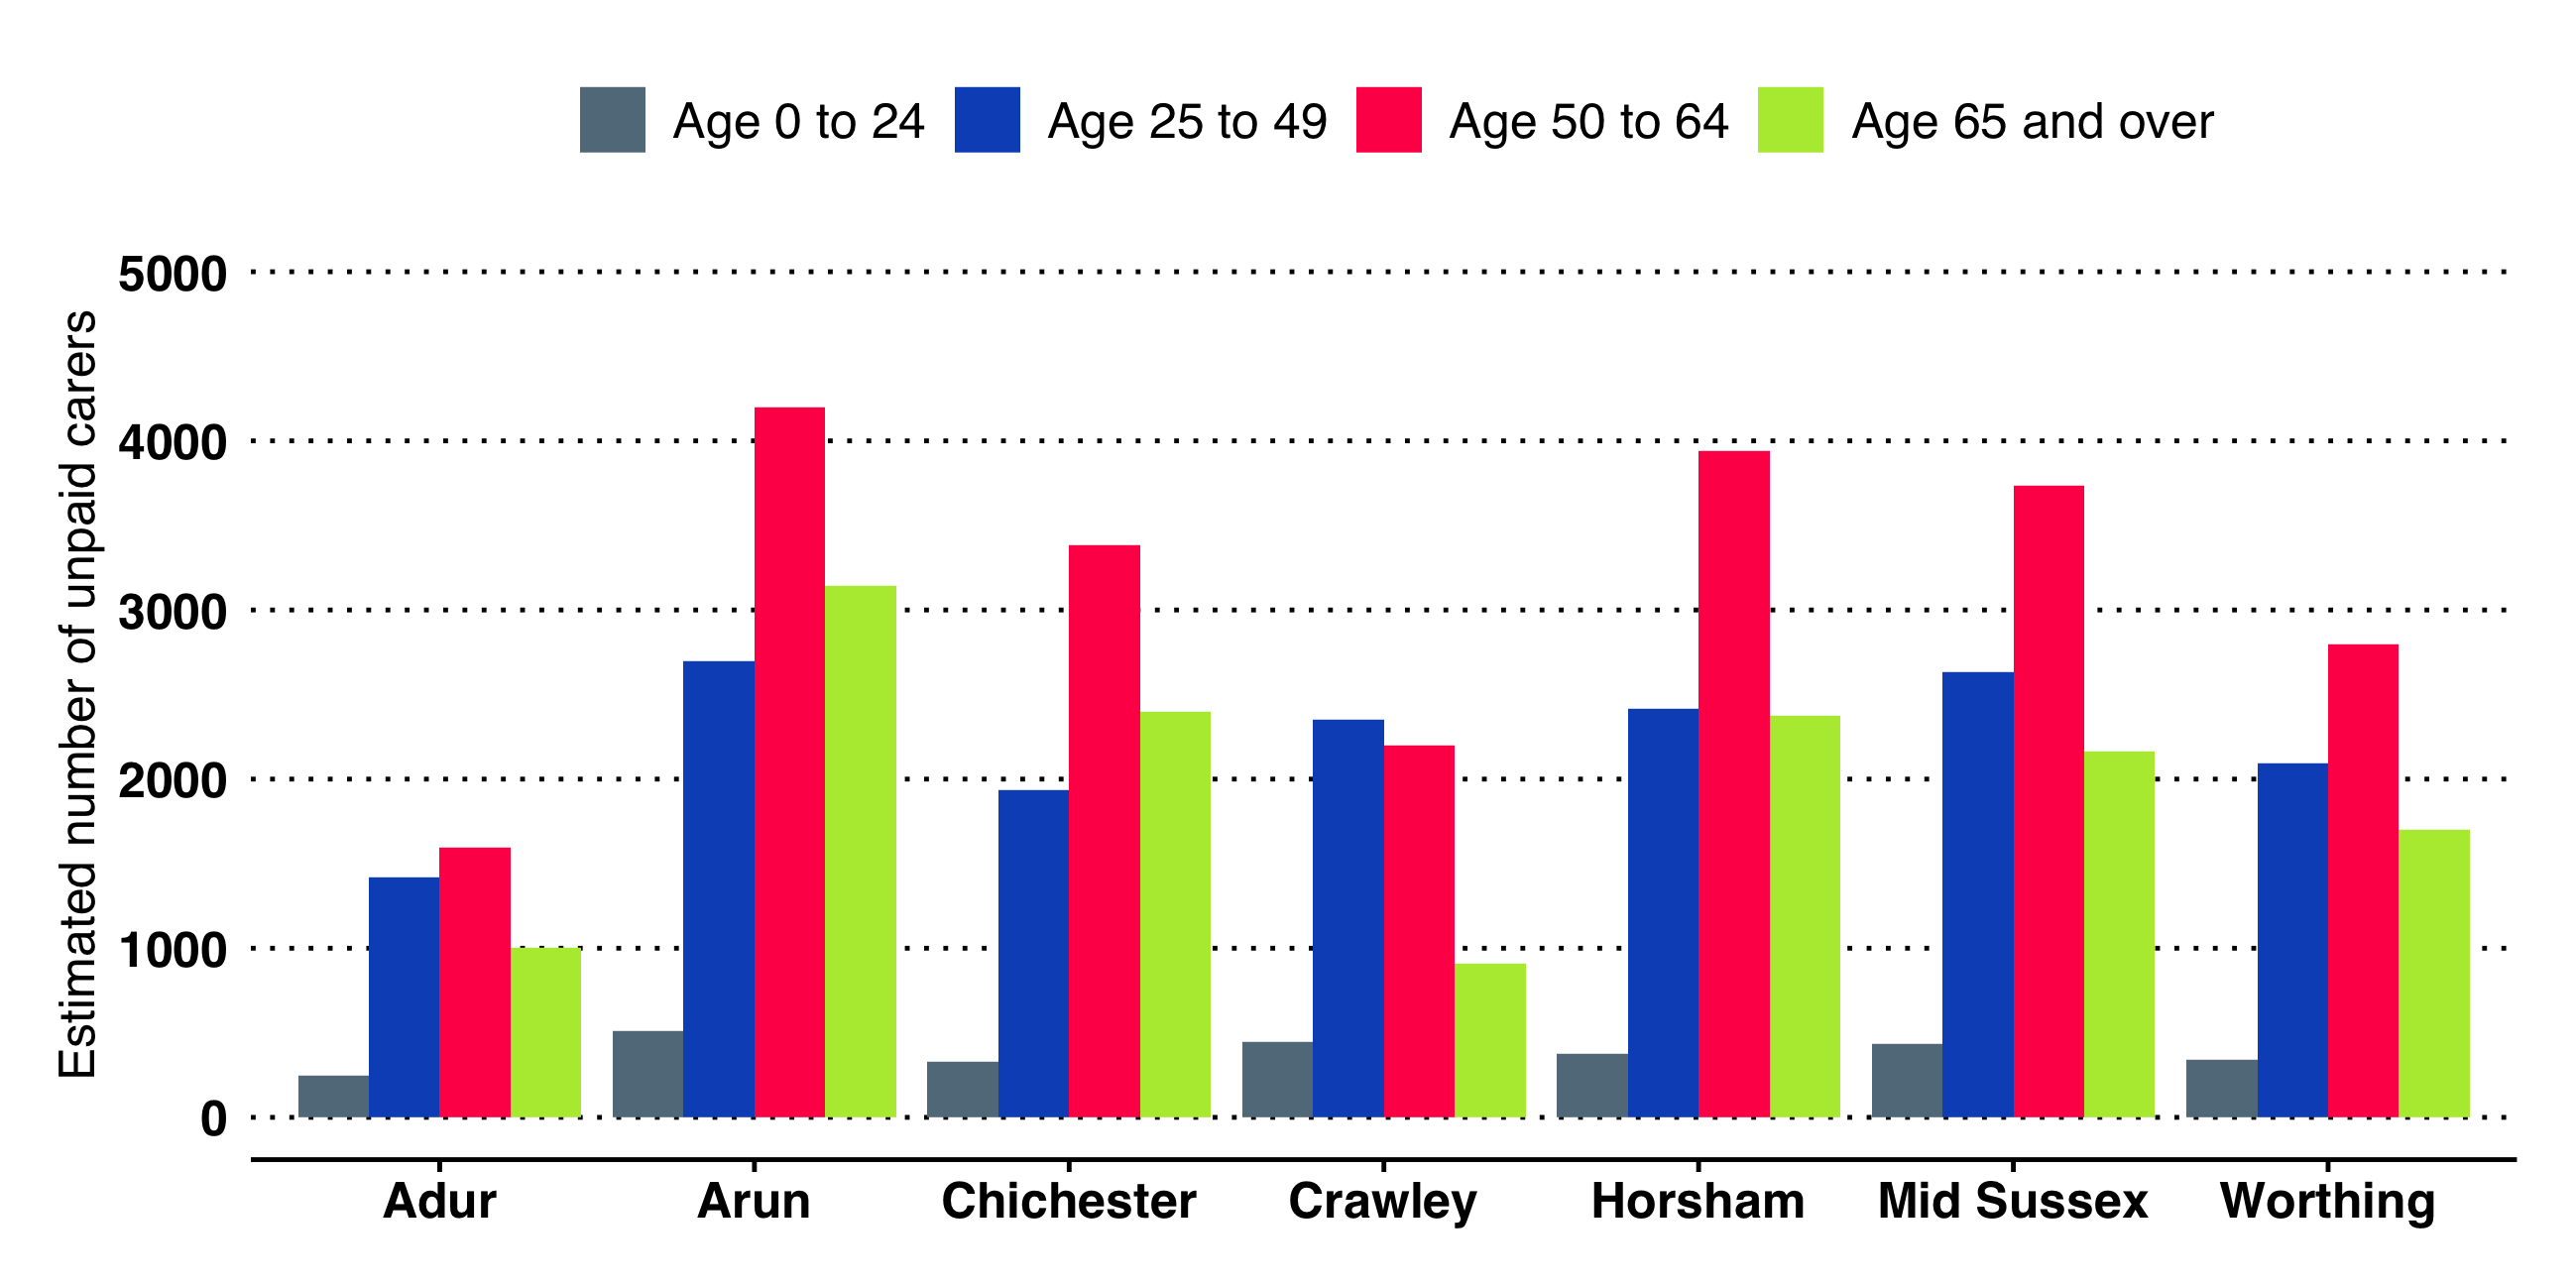
\includegraphics[width=\linewidth]{images/female_unpaid_carers.png}
    \end{subfigure}
    \begin{subfigure}[b]{0.99\linewidth}
        \centering
        \caption{Male carers by West Sussex Local Authorities.}\label{fig:unpaidcarers:dabs:male}        
        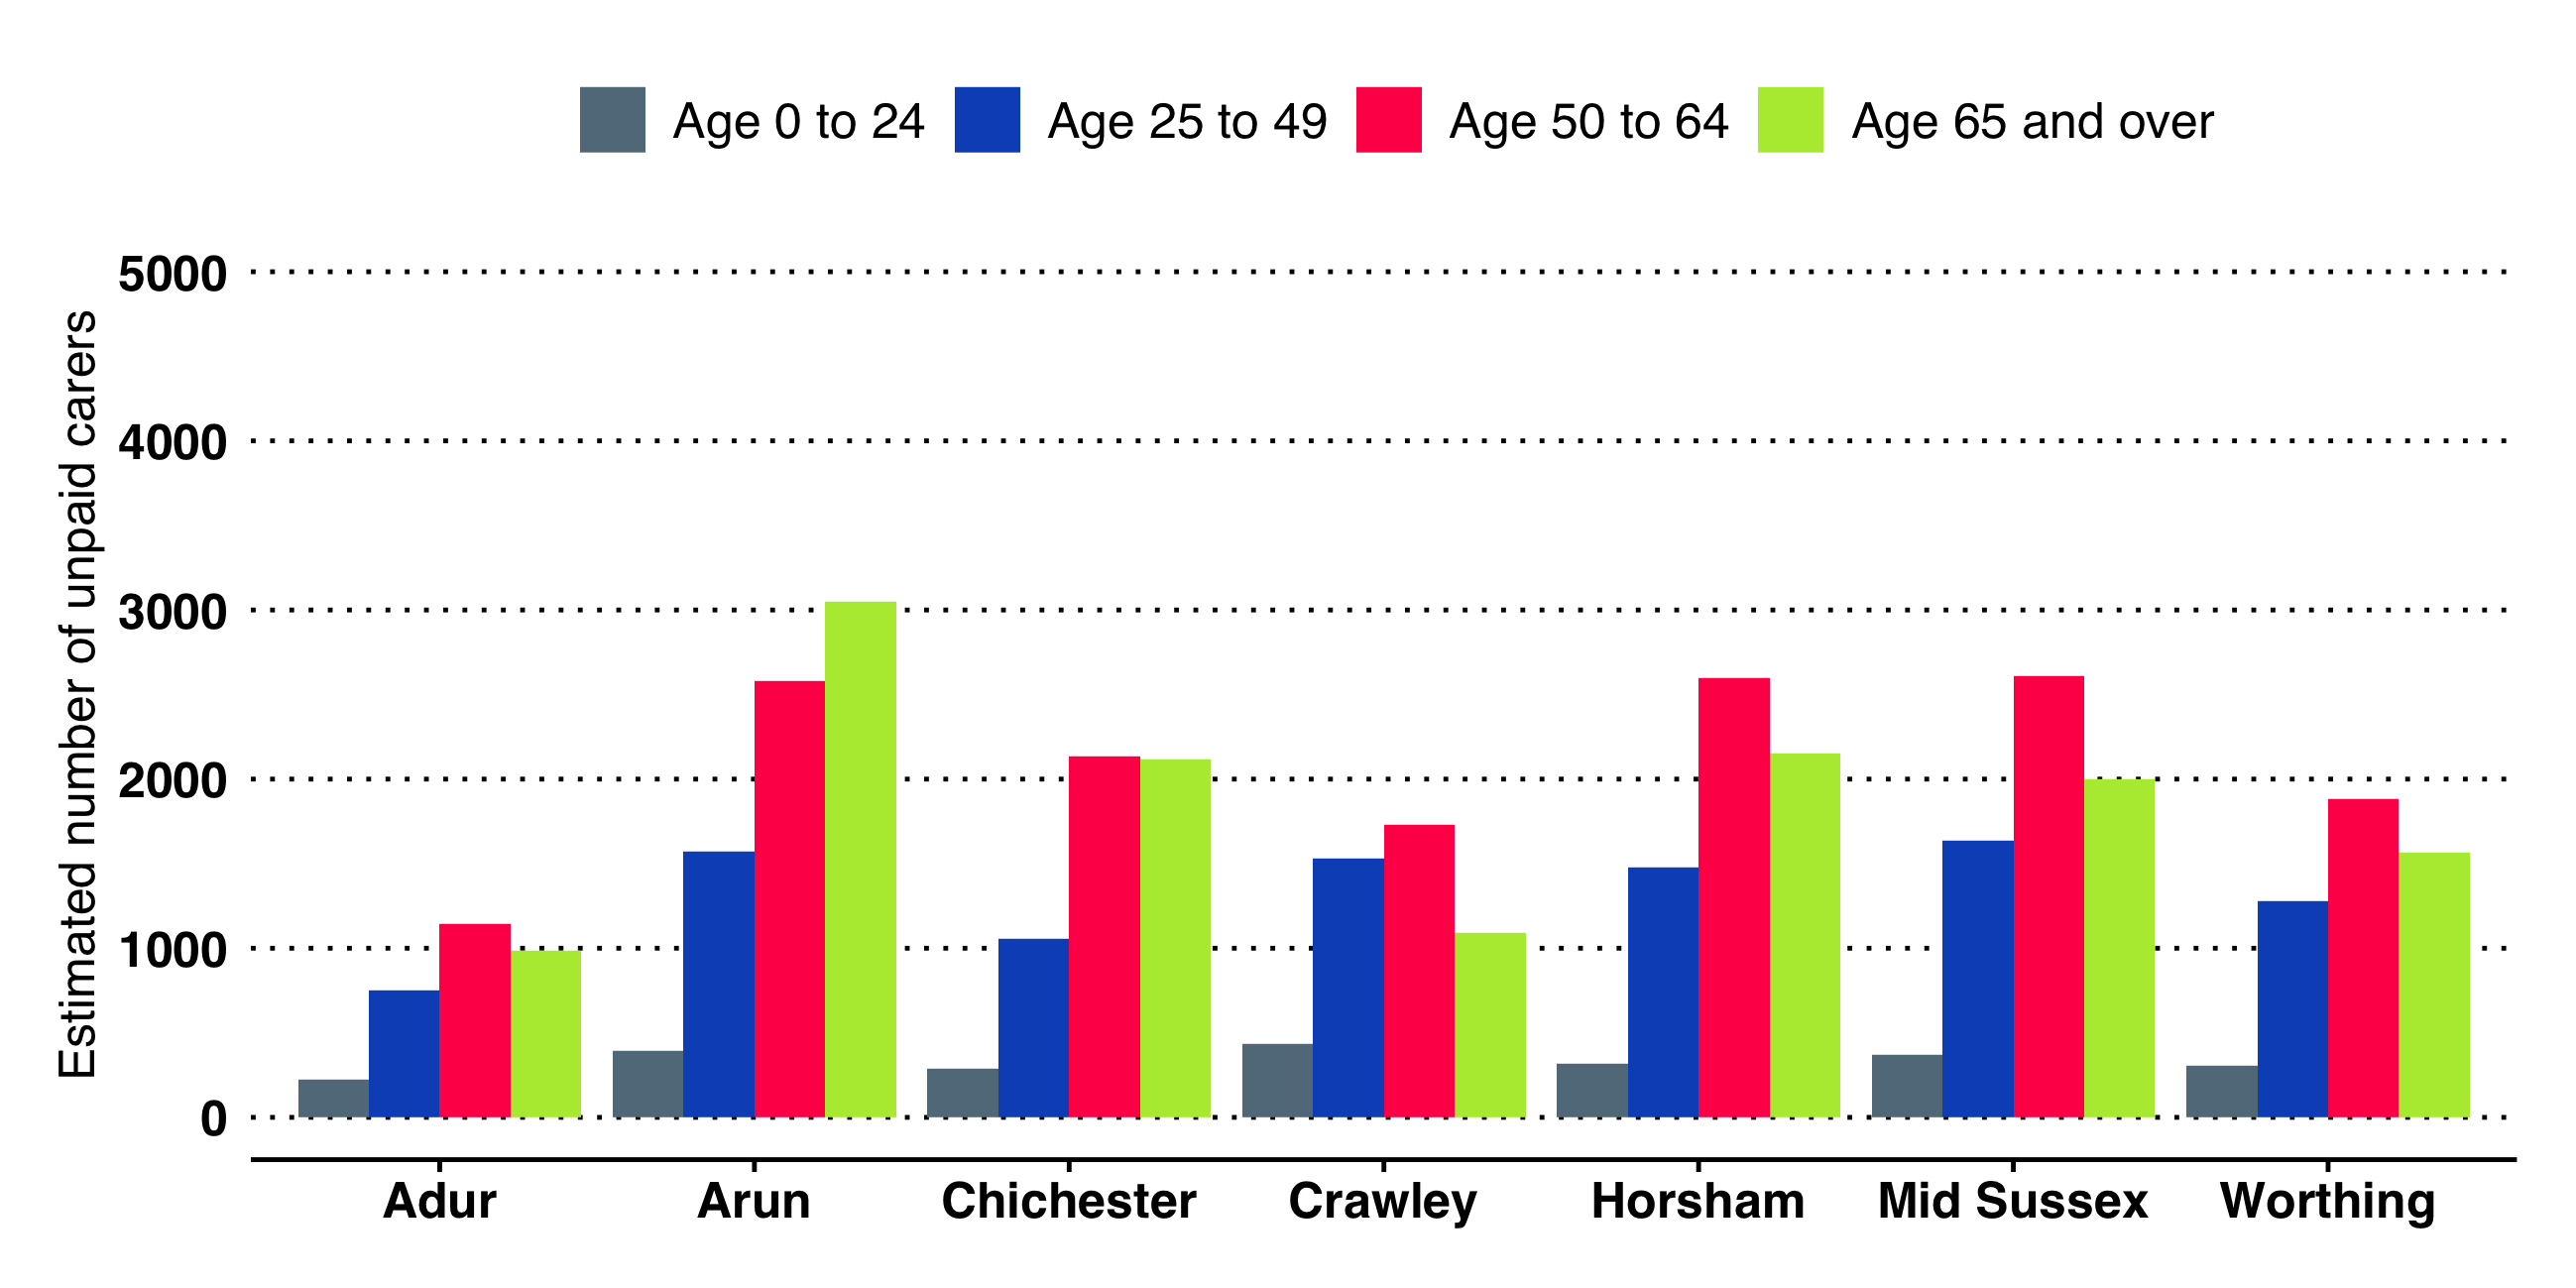
\includegraphics[width=\linewidth]{images/male_unpaid_carers.png}
    \end{subfigure}
    \vspace*{3mm}
\end{figure}

% \paragraph{Carers in the GP Patient Survey} Results from the GP Patient Survey 2019 are shown at West Sussex Clinical Commissioning Group and West Sussex level and compare the experiences of carers and non-carers. Note: these data relate to people registered with a GP Practice who responded to the survey. 

% \begin{itemize}[noitemsep]
%     \item As a proportion of patients, West Sussex has significantly more carers compared to England (18\% vs. 16.9\% of patients), particularly in the Coastal West Sussex CCG (19.3\%).
%     \item The highest proportion of carers was amongst the middle-age groups (45-54 and 55-64 years), with roughly one in four patients in these age-groups providing some care. Compared to England, the proportion of carers aged 55-64 years is higher in West Sussex, and the proportion of 16-24 and 25-34 year olds lower.
%     \item In each West Sussex CCG, over half of carers said they provided support for 1 to 9 hours per week, whilst around one in five carers provided 50 or more hours per week, similar to England.
% \end{itemize}
  
% FIGURE Proportion of carers by number of hours of care provided per week

% \paragraph{Working status} Carers were significantly less likely to be in full-time paid employment compared to non-carers (all ages) in all areas except NHS Horsham and Mid Sussex CCG.

% More carers were looking after the family or home or in part-time paid work than non-carers. However, compared to carers in England, carers in West Sussex were significantly less likely to be in full-time education, looking after the family home, permanently sick or disabled, or unemployed.

% \paragraph{Long-term conditions} Significantly more carers report having a long-term condition (LTC), disability or illness in West Sussex, at 62.5\% of carers compared to around 50\% of non-carers. This proportion is significantly higher, at 65.1\%, in the Coastal West Sussex CCG.

% In West Sussex and England, more carers reported musculoskeletal conditions (arthritis or ongoing problems with back and joints) and long- term mental health issues.

% There was no significant difference in current smoking prevalence between carers and non-carers, and prevalence in West Sussex was significantly lower than England.

% \paragraph{Making Appointments} Fewer carers reported an overall good experience of making an appointment compared to non-carers (63.3\% compared to 69.2\%; similar to England).

% The proportion of patients satisfied with the type of appointment offered was significantly lower amongst carers compared to non-carers, at 71.6\% compared to 76.6\% (similar to England).

% In all areas a except the Crawley CCG, a significantly higher proportion of carers had attempted to access an NHS service when their GP practice was closed, either for themselves or someone else, compared to non-carers.

% A significantly higher proportion of carers had a preferred GP compared to non-carers in all areas (58.1\% Vs. 48.8\%), except the Crawley CCG, although fewer carers reported seeing their preferred GP always or almost always, at 19.1\% VS. 24.3\% of non-carers. This proportion of carers seeing their preferred GP was also significantly lower in West Sussex compared to England (22\%).

\subsection{Health Related Behaviours}
\paragraph{Lifestyle risk factors: smoking; diet; physical activity; and alcohol and other substance misuse.}

West Sussex is relatively healthy with lower levels of "riskier behaviour". However this masks considerable differences between areas, and between groups within the county.

We know that there is a clustering of behaviours; people who smoke are more likely to drink above recommended levels and have lower physical activity rates and so on. This means that there is polarisation taking place, with people who take on key health messages and take steps to lead healthier lives and those who do not. This acts to reinforce and increase existing inequalities.

\paragraph{Smoking}
The following data have been taken from the PHE Local Tobacco Control Profiles. These profiles bring together the range of measures which examine the effects and wider impact of smoking, including prevalence rates, smoking quits and attributable mortality. \url{https://fingertips.phe.org.uk/profile/tobacco-control}

Smoking the remains biggest cause of premature deaths in West Sussex and smoking attributable mortality. There were 3,049 deaths attributed to smoking over the 3 year period between 2017 and 2019.

The overall adult smoking rate in the county has continued to fall. In 2020 the rate was estimated at 11.2\% (CI 8.5\% to 13.9\%)\footnote{PHOF reference C18.} - meaning almost 80,000 people in the county still smoke.

{\bfseries Declines in the smoking rates of people from routine and manual occupations have been smaller.} The most recent survey (2020) estimated the odds of current smoking in West Sussex among routine and manual workers aged 18-64 at 2.0 (CI: 1.2 to 3.4), meaning that prevalence among routine and manual workers could be between 13.4\% and 38.1\%.

In 2020, around a third of people in West Sussex aged 18+ reported being ex-smokers, while 56.4\% reported never having smoked.

\paragraph{Physical Activity and Obesity}
\begin{itemize}[noitemsep]
    \item An estimated 70.2\% of adults were classed as physically active\footnote{PHOF reference C17a. These are adults (aged 19+) who meet CMO recommendations for physical activity (150+ moderate intensity equivalent minutes per week).}. This is higher than England and the average of statistical neighbours. (2020/21 survey data).
    \item 20\% of adults were physically inactive\footnote{PHOF reference C17b. These are adults (aged 19+) that are physically inactive (<30 moderate intensity equivalent minutes per week).}.
    \item The proportion of the adult population meeting the recommended '5-a-day' portions of fruit and vegetables on a 'usual day'\footnote{PHOF reference C15.} in West Sussex was 60.6\%. This is higher than the England rate. Within West Sussex, the majority of districts and boroughs had a rate significantly higher than England, though Arun, Adur, and Crawley are similar to England.
    \item 63.8\% of adults were overweight or obese\footnote{PHOF reference C16.} in West Sussex, similar to comparable authorities and England. In Adur, rates were higher than England whilst the other districts and boroughs were similar to England.
\end{itemize}

\begin{figure}[h]
    \caption{Percentage of overweight or obese adults - West Sussex Local Authorities, 2020/21}\label{fig:obesity:rag}
    \centering
    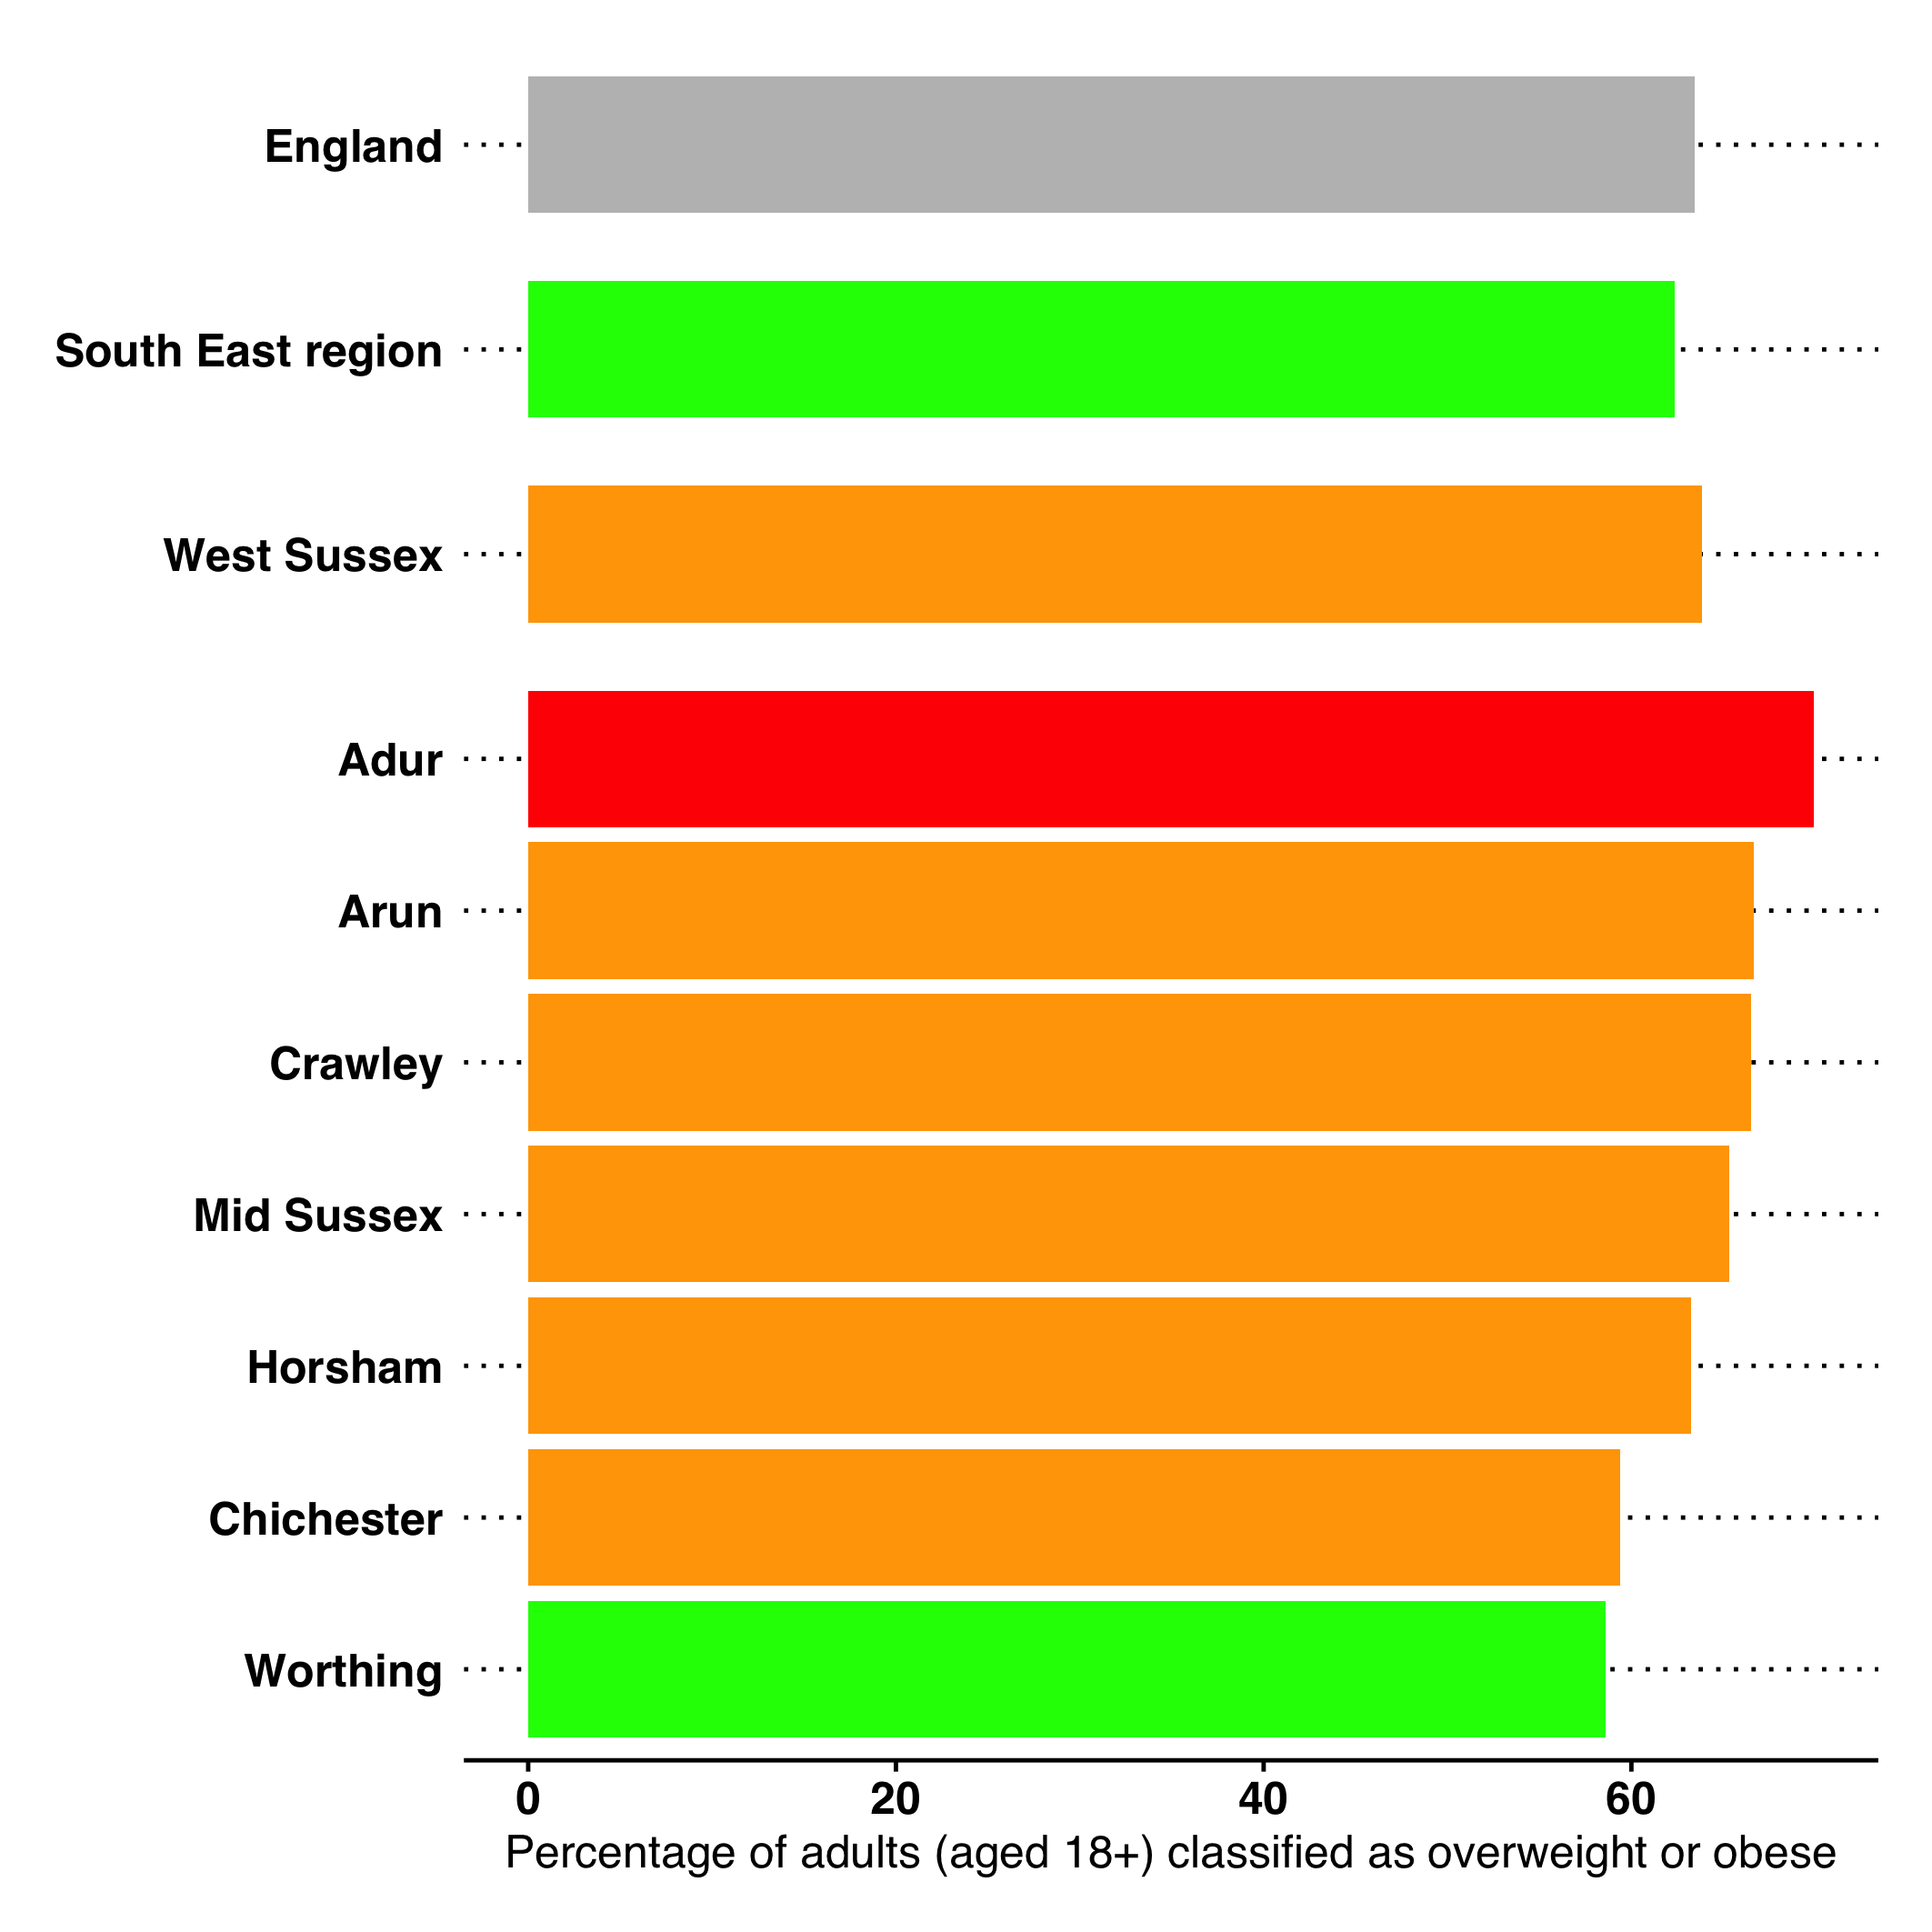
\includegraphics[width=\linewidth]{images/obesity_rag_bar.png}
\end{figure}

\subsection{Substance Misuse}
\subsubsection{Tobacco}
\paragraph{West Sussex Tobacco Control Strategy 2019-2022} Smoking remains the single biggest preventable cause of death and ill health in England. Any differences in smoking prevalence across the population inevitably translate into health inequalities.

The Smokefree West Sussex Partnership is a group of organisations across West Sussex working in partnership to provide strategic direction and leadership on the tobacco control agenda in West Sussex. The West Sussex Tobacco Control Strategy 2019-2022 contributes to realising the Public Health vision for West Sussex and meeting the national objectives through the co-ordinated effort of a wide range of partners. The strategy builds on national plans which establish tobacco control as a comprehensive and coordinated effort to reduce demand, prevent uptake, and support cessation rather than a sole focus on the delivery of smoking cessation services.

The details of the full strategy document and action plan can be found on the JSNA website. An additional website (\url{https://sfws-action-plan.netlify.com/}) provides an interactive version of the strategy to support partners in understanding what actions can be taken, and by who in the short-, medium- and longer- term. 

\subsubsection{Substance Misuse - Alcohol and Drugs} Prevalence Estimates Alcohol-related harm is affected by the amount of alcohol that is consumed and how it is consumed (frequency and intensity of use). Describing patterns of use is therefore complicated. This diagram\footnote{Source: Public Health England, The Public Health Burden of Alcohol and the Effectiveness and Cost-Effectiveness of Alcohol Control Policies An evidence review, 2016} sets out the various terms and estimates (at a national level).

%FIGURE - Diagram describing patterns of alcohol use and misuse from PHE

\begin{itemize}[noitemsep]
    \item {\bfseries Abstainers}
    \item {\bfseries Lower Risk Drinking} - drinking less than 14 units per week
    \item {\bfseries Increasing Risk Drinking} - drinking 14 to 50 units a week
    \item {\bfseries Higher Risk Drinking} 50+ units for men a week / 35+ units for women a week
    \item {\bfseries Binge drinking} - drinking of 8+ units (men) / 6+ units (women) on heaviest drinking day in previous week
    \item {\bfseries Dependent Drinkers} - this is derived from data collected as part of the Adult Psychiatric Morbidity Survey (APMS), a national survey of 16+ year-olds. Alcohol dependency is assessed by the Alcohol Use Disorders Identification Test (AUDIT) and the Severity of Alcohol Dependence Questionnaire (SADQ).
\end{itemize}

At {\bfseries West Sussex level} using data from the Health Survey for England (2011 to 2014): 

\begin{itemize}[noitemsep]
    \item 9.6\% of the 18+ population are estimated to be {\bfseries abstainers} - equivalent to 66,600 people in West Sussex (2020 population estimates).
    \item 14.5\% of the 18+ population are estimated to be {\bfseries binge drinkers} - equivalent to 100,700 people in West Sussex.
    \item 23.7\% of the 18+ population are estimated to be {\bfseries drinking 14+ units a week} - equivalent to 168,900 people in West Sussex.
\end{itemize}

Using the APMS, it is estimated that there are 5,500 to 9,300 people in West Sussex with a dependency on alcohol and potentially in need of specialist treatment.

% More up-to-date figures on alcohol misuse needed, especially during and after lockdowns 

\subsubsection{Treatment Outcomes / Impact}
Some of the following data have been taken from the PHE Local Alcohol Profiles for England. These profiles bring together the range of measures which examine the effects and wider impact of alcohol, including alcohol related admissions to hospital, attributable mortality and road accidents.\footnote{\url{https://fingertips.phe.org.uk/profile/local-alcohol-profiles}}

PHE also publish annual estimates of the prevalence of opiate use and/or crack cocaine use. However, data at county level and for specific age groups have not been updated since March 2019. The values presented here are taken from OHID Fingertips.

\paragraph{Alcohol-Related Hospital Admissions} Each rate is for all ages, directly age standardised and measured per 100,000 population. West Sussex compares favourably with England for each rate and is lower than most statistical neighbours. Note that only the specific definition has been updated since 2019.
\begin{itemize}[noitemsep]
    \item There were 583 admissions for alcohol-related conditions (Narrow)\footnote{PHOF reference C21.} per 100,000 (England 664 per 100,000). The number of such admissions in West Sussex was 5,116.
    \item There were 1,887 admissions for alcohol-related conditions (Broad) per 100,000 (England 2,367 per 100,000). The number of such admissions in West Sussex was 17,301.
    \item There were {\bfseries 480 admissions for alcohol-related conditions (Specific) per 100,000} (England 587 per 100,000). The number of such admissions in West Sussex was 4,230.
\end{itemize}
  
\paragraph{Other alcohol-related impacts}
Between 2014 and 2016 there were 206 alcohol-related road traffic accidents in which at least one driver failed a breath test. This represents a rate of 33.8 per 1,000 accidents and is higher than the England rate (26.4) but in line with other comparable local authorities.

\paragraph{Mortality from chronic liver disease} Mortality from chronic liver disease\footnote{PHOF reference E06b}, which is strongly associated with alcohol consumption and obesity, has risen in West Sussex. Recent mortality rates for men and women were significantly lower than the England rate, but this is no longer the case. Using a three year range, the rate is now similar to that of England. Nationally there is evidence that deaths from liver disease are occurring at younger ages.

\begin{figure}[ht]
    \caption{Mortality from chronic liver disease per 100,000 population (All persons, 3 year range)}
    \centering
    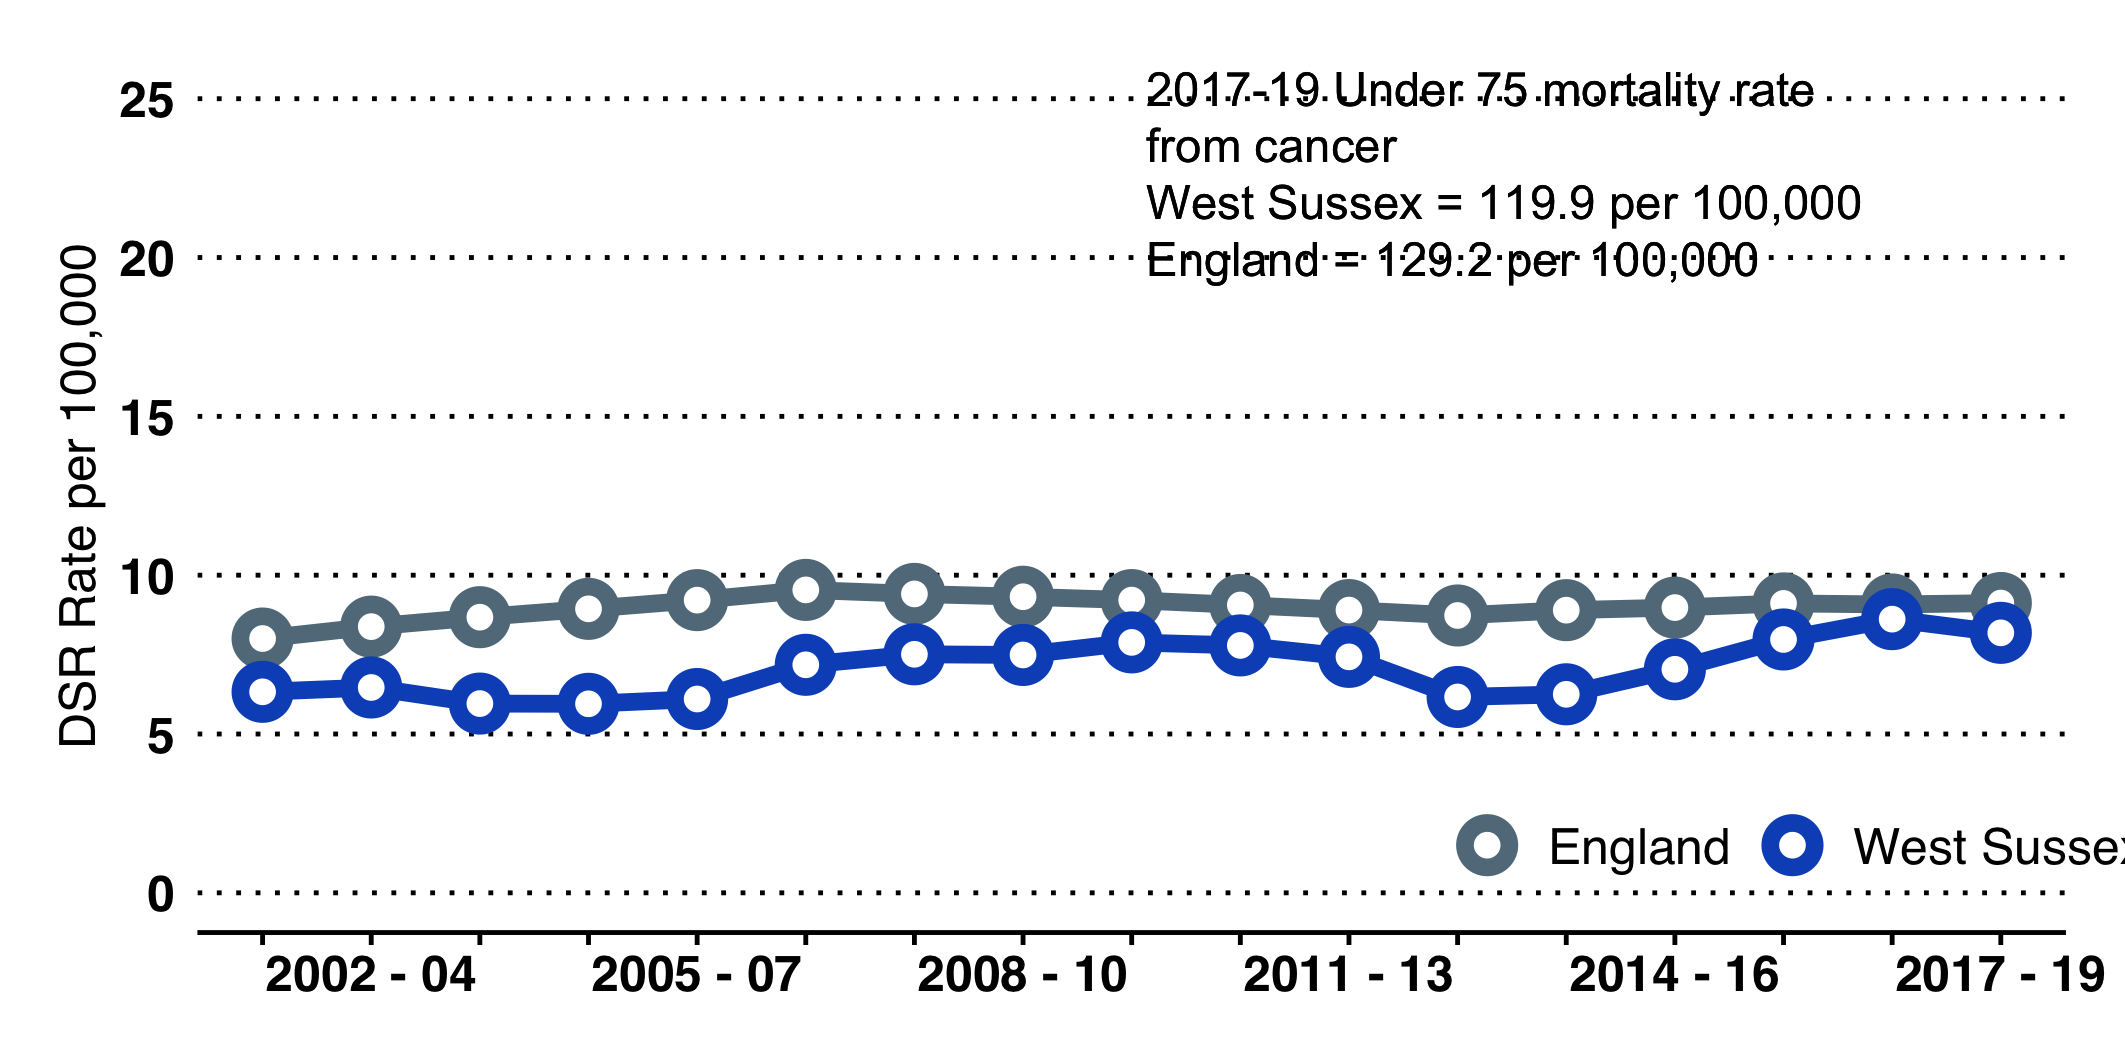
\includegraphics[width=\linewidth]{images/u75_liver_line.png}
    \label{fig:u75_liver}
\end{figure}

\paragraph{Drug misuse} It is estimated that between 1,400 and 4,100 people (aged 16-64 years) use opiates and/or crack in West Sussex, 70\% of which are 35 years or older. In 2018-2020, there were 78 deaths in West Sussex classified as drug misuse deaths\footnote{PHOF reference C19d}. Although the rate of drug related deaths in West Sussex remains lower than the England rate (3.2 per 100,000 compared to 5.0 nationally) a recent upward trend has begun to stabilise.

\paragraph{Treatment Outcomes}
There have been improvements in recent years in the successful completion rates of treatment in West Sussex. Note there is a time lag on these measures and numbers are low - notably for opiate drug users.

\begin{itemize}[noitemsep]
    \item 32.9\% of {\bfseries alcohol users} that left treatment successfully\footnote{PHOF reference C19c} in 2020 did not re-present to treatment within 6 months (England rate 35.3\%). This is similar to other comparable local authorities (33.7\%).
    \item 31.4\% of {\bfseries non-opiate drug users} who left treatment successfully\footnote{PHOF reference C19b} did not re-present to treatment within 6 months (England rate 33.0\%). This has improved in recent years, with the rate similar to England and comparable local authorities (34.5\%).
    \item 5\% of opiate drug users who left treatment successfully\footnote{PHOF reference C19a} did not re-present to treatment within 6 months (England rate 4.6\%). This is similar to the England rate but less than the average of  comparable local authorities (5.7\%, CI: 5.4\%-6.1\%).
\end{itemize}

\paragraph{People NOT in Receipt of Treatment (2018/19)} Using prevalence estimates and data from treatment services (from the National Drug Treatment Management System (NDTMS)), we can estimate the percentage of people with an alcohol dependency and users of opiates and/or crack cocaine (OCU) who are not in receipt of treatment.

\begin{itemize}[noitemsep]
    \item The estimated proportion of the West Sussex OCU users in 2018/19 who were {\bfseries not in contact with drug treatment services for an OCU problem was 51\%} (approximately 1,350 people).
    \item The estimated proportion of the West Sussex dependent drinkers in need of specialist alcohol treatment who were {\bfseries not in contact with treatment services for alcohol only or alcohol and non-opiate use was 78.3\%} (approximately 5,600 people).
\end{itemize}
 
\paragraph{Drug Use} The Royal Society for Public Health report 'Taking a New Line on Drugs' (2016)\footnote{Source: RSPH Taking a New Line in Drugs \url{https://www.rsph.org.uk/our-work/campaigns/taking-a-new-line-on-drugs.html}} sets out the challenge of reducing drug-related harm.

It notes that:

\begin{itemize}[noitemsep]
    \item Many substances that cause harm are legal and socially embedded, including alcohol, tobacco and prescription drugs.
    \item Harm is multi-faceted, including harm to individuals, others and the wider society.
    \item The relationship between drugs and mental health is complex. People may use drugs for a psychological effect and use can result in feelings of anxiousness, depression etc.
    \item Some people are at a higher risk of drug use and harm than others. People with pre-existing mental health conditions, including anxiety and depression, are particularly at risk.
    \item Drug harm can affect all ages and communities, but it is known that harm disproportionately affects people from more deprived communities.
\end{itemize}

%\subsection{A Focus on Drug Related Deaths}
%\paragraph{Background} In 2016, Public Health England released a report into the sharp rise of Drug Related Deaths (DRDs) seen between 2013 and 2015, which reached the highest national levels yet seen in 2015\footnote{PHE (2016). Understanding and preventing drug-related deaths: The report of a national expert working group to investigate drug-related deaths in England}. This included a 21\% increase in 2013 and a 17\% increase in 2014. ONS figures also indicated a 64\% increase in heroin-related death registrations from 2013 to 2015. The subsequent 2017 West Sussex Suicide Audit, which examined deaths between 2013 and 2015, revealed 42 individuals had taken their own lives by self -poisoning (20\% of all suicides in the three-year period).

%\paragraph{West Sussex Drug Related Deaths} The newly designed West Sussex Drug Related Deaths Audit covered the period between 1st January 2015 to 31 st December 2017 and reviewed 123 deaths. Although Public Health teams and Commissioning managers collect data on those who have died whilst connected to community services, which are essential to preventing early death, this alone does not provide insight into the wider population or the individuals identified in this audit who were not involved with services at any point. Examining the barriers and facilitators to service engagement can help in refocusing efforts to engage with more residents.

%The full report of the audit is available on the JSNA website. Contact Robert Whitehead (\url{robert.whitehead@westsussex.gov.uk}) for more information.

%\subsubsection{Key points}
%\begin{itemize}[noitemsep]
%    \item There were 123 deaths from drug poisonings in the three-year period the audit examined. Over a quarter of these were suicides and more than half were accidental overdoses. Roughly half of all deaths were classed as drug misuse.
%    \item Males accounted for two thirds of all deaths. Half of these involved controlled substances and males accounted for 86\% of all drug misuse deaths, particularly focused between ages of 25 and 44 years.
%    \item Female deaths were spread more evenly among older age groups and were explained by a higher proportion of accidental overdoses and suicides involving prescribed medications. Drug misuse was ascribed to 24\% of female deaths.
%    \item Eight males had been in prison or involved with probation services in the past year (9\% of male deaths).
%    \item Ten males were known to be homeless or of no fixed abode (16\% of all drug misuse deaths).
%    \item Four in every five deaths occurred in the home or the home of another. Only 9\% of deaths occurred in a public area.
%    \item There was an increase in overdoses on Saturdays and suicides on Sundays.
%    \item Evidence around Naloxone intervention and resuscitation attempts were not sufficiently documented to report on in this audit.
%\end{itemize}

\subsection{Sexual Health}
%To inform the re-procurement of local sexual health services, a detailed needs assessment was undertaken in 2019. This is available on the JSNA website. On the next few pages are a selected number of metrics from the needs assessment, many of which are from the Public Health Outcomes Framework. The latest published data are available in the local Sexual and Reproductive Health Profile on PHE Fingertips.

%For further information contact Dr Matthew Dorey (\url{matthew.dorey@westsussex.gov.uk}).

\paragraph{Key Points} In 2020, there were a total of 2,984 new STI diagnoses (all STIs), a rate of 344 per 100,000 population. This is a large decrease compared to 2019, which had the highest rate of new diagnoses in West Sussex in the previous 5 years, and below the national rate (562 per 100,000) along with comparable local authorities. While local services did provide an online service supplying self-testing kits, it is likely that the number of diagnoses is a result of Covid-19. 

\begin{table}
    \caption{Number and rate of specific STI diagnoses in West Sussex, 2020.}
    \centering
    \begin{tabular}{llll}
    \toprule
    STI & Number of diagnoses & Rate (West Sussex) & Rate (England) \\
    \midrule
    Chlamydia & 1336 & 154 & 286 \\
    Genital warts & 455 & 52.4 & 48.6 \\
    Genital herpes & 330 & 38 & 36 \\
    Gonorrhoea & 351 & 40 & 101 \\
    Syphilis & 84 & 9.7 & 12.2 \\
    \bottomrule
    \end{tabular}
    \label{tab:wa:stis}
\end{table}

Rates of new STI diagnoses for Chlamydia, Gonorrhea, Syphilis, Genital Herpes and Genital Warts are consistently below the England rate. However, the rates of the former three have been increasing over the past ten years, at a similar rate of increase to England. Compared to similar authorities, diagnosis rates for Gonorrhea, Herpes and Syphilis in West Sussex are amongst the highest.

The overall testing rate (excluding for Chlamydia in under 25s), a metric strongly associated with the level of diagnoses, was 3583.7 per 100,000 in 2020, remaining significantly lower than the England rate (4549.3 per 100,000) and 9th highest amongst CIPFA neighbours.

The proportion of late HIV diagnoses (i.e. where the CD4 cell count is less than 350 per $\mathsf{mm}^3$)\footnote{PHOF reference D07. Late diagnosis is the most important predictor of morbidity and mortality among those with HIV infection.} has increased in recent years, to approximately 52\% in 2018 - 2020. This is higher than England (42.4\%) and equates to 50 late HIV diagnoses in West Sussex between 2018 - 2020.

%Overall attendances at sexual health venues increased from 24,300 to 28,900 between 2013 and 2017. The proportion of people receiving a sexual health screen on first attendance increased from 68\% to 79\% over the same time period.

In 2020, there were 148 conceptions in under-18 year-olds\footnote{PHOF reference C02a.}, a slight decrease on 2019. The rate of 11.1 per 1,000 15-17 year-olds is similar to England. 63\% of teenage conceptions ended in abortion in West Sussex (England, 53\%).

In 2020, the rate of abortions per 1,000 females aged 15-44 in West Sussex was 17.1, in line with comparable authorities and below the England rate (18.9/1,000), although higher than the previous 8 years. The percentage of abortions undertaken under 10 weeks in West Sussex is, at 88.7\%, similar to England (88.1\%) and 7th lowest amongst comparable authorities. Of the abortions to women aged under 25 years, 25.3\% (212 abortions) were repeat abortions i.e. to women who had had previous abortions.

The use of long acting reversible contraception\footnote{PHOF reference C01. This measure excludes LARC injections.} in West Sussex is relatively high (51.6 per 1,000 female population aged 15-44 years in 2020) compared with similar authorities and England (34.6/1,000). All rates are considerably lower than 2019, highlighting the difficulty of accessing these services during the Covid-19 pandemic.

The hospital admission rate for Pelvic Inflammatory Disease (PID) in West Sussex has been high in recent years. Between 2016/17 and 2019/20, admissions rates were significantly higher than the England rate. In 2019/20 the rate in West Sussex the rate was 329.9 per 100,000 compared to 254.7 per 100,000 in England. Rates fell significantly in both West Sussex and England during 2020/21, with the rate for West Sussex 191.6 per 100,000 higher than that for England (186.2 per 100,000).
 
\begin{figure}[ht]
    \caption{Teenage conceptions have steadily declined in the last 20 years, although two of the past three years have seen small increases.}\label{fig:teen_conc}
    \centering
    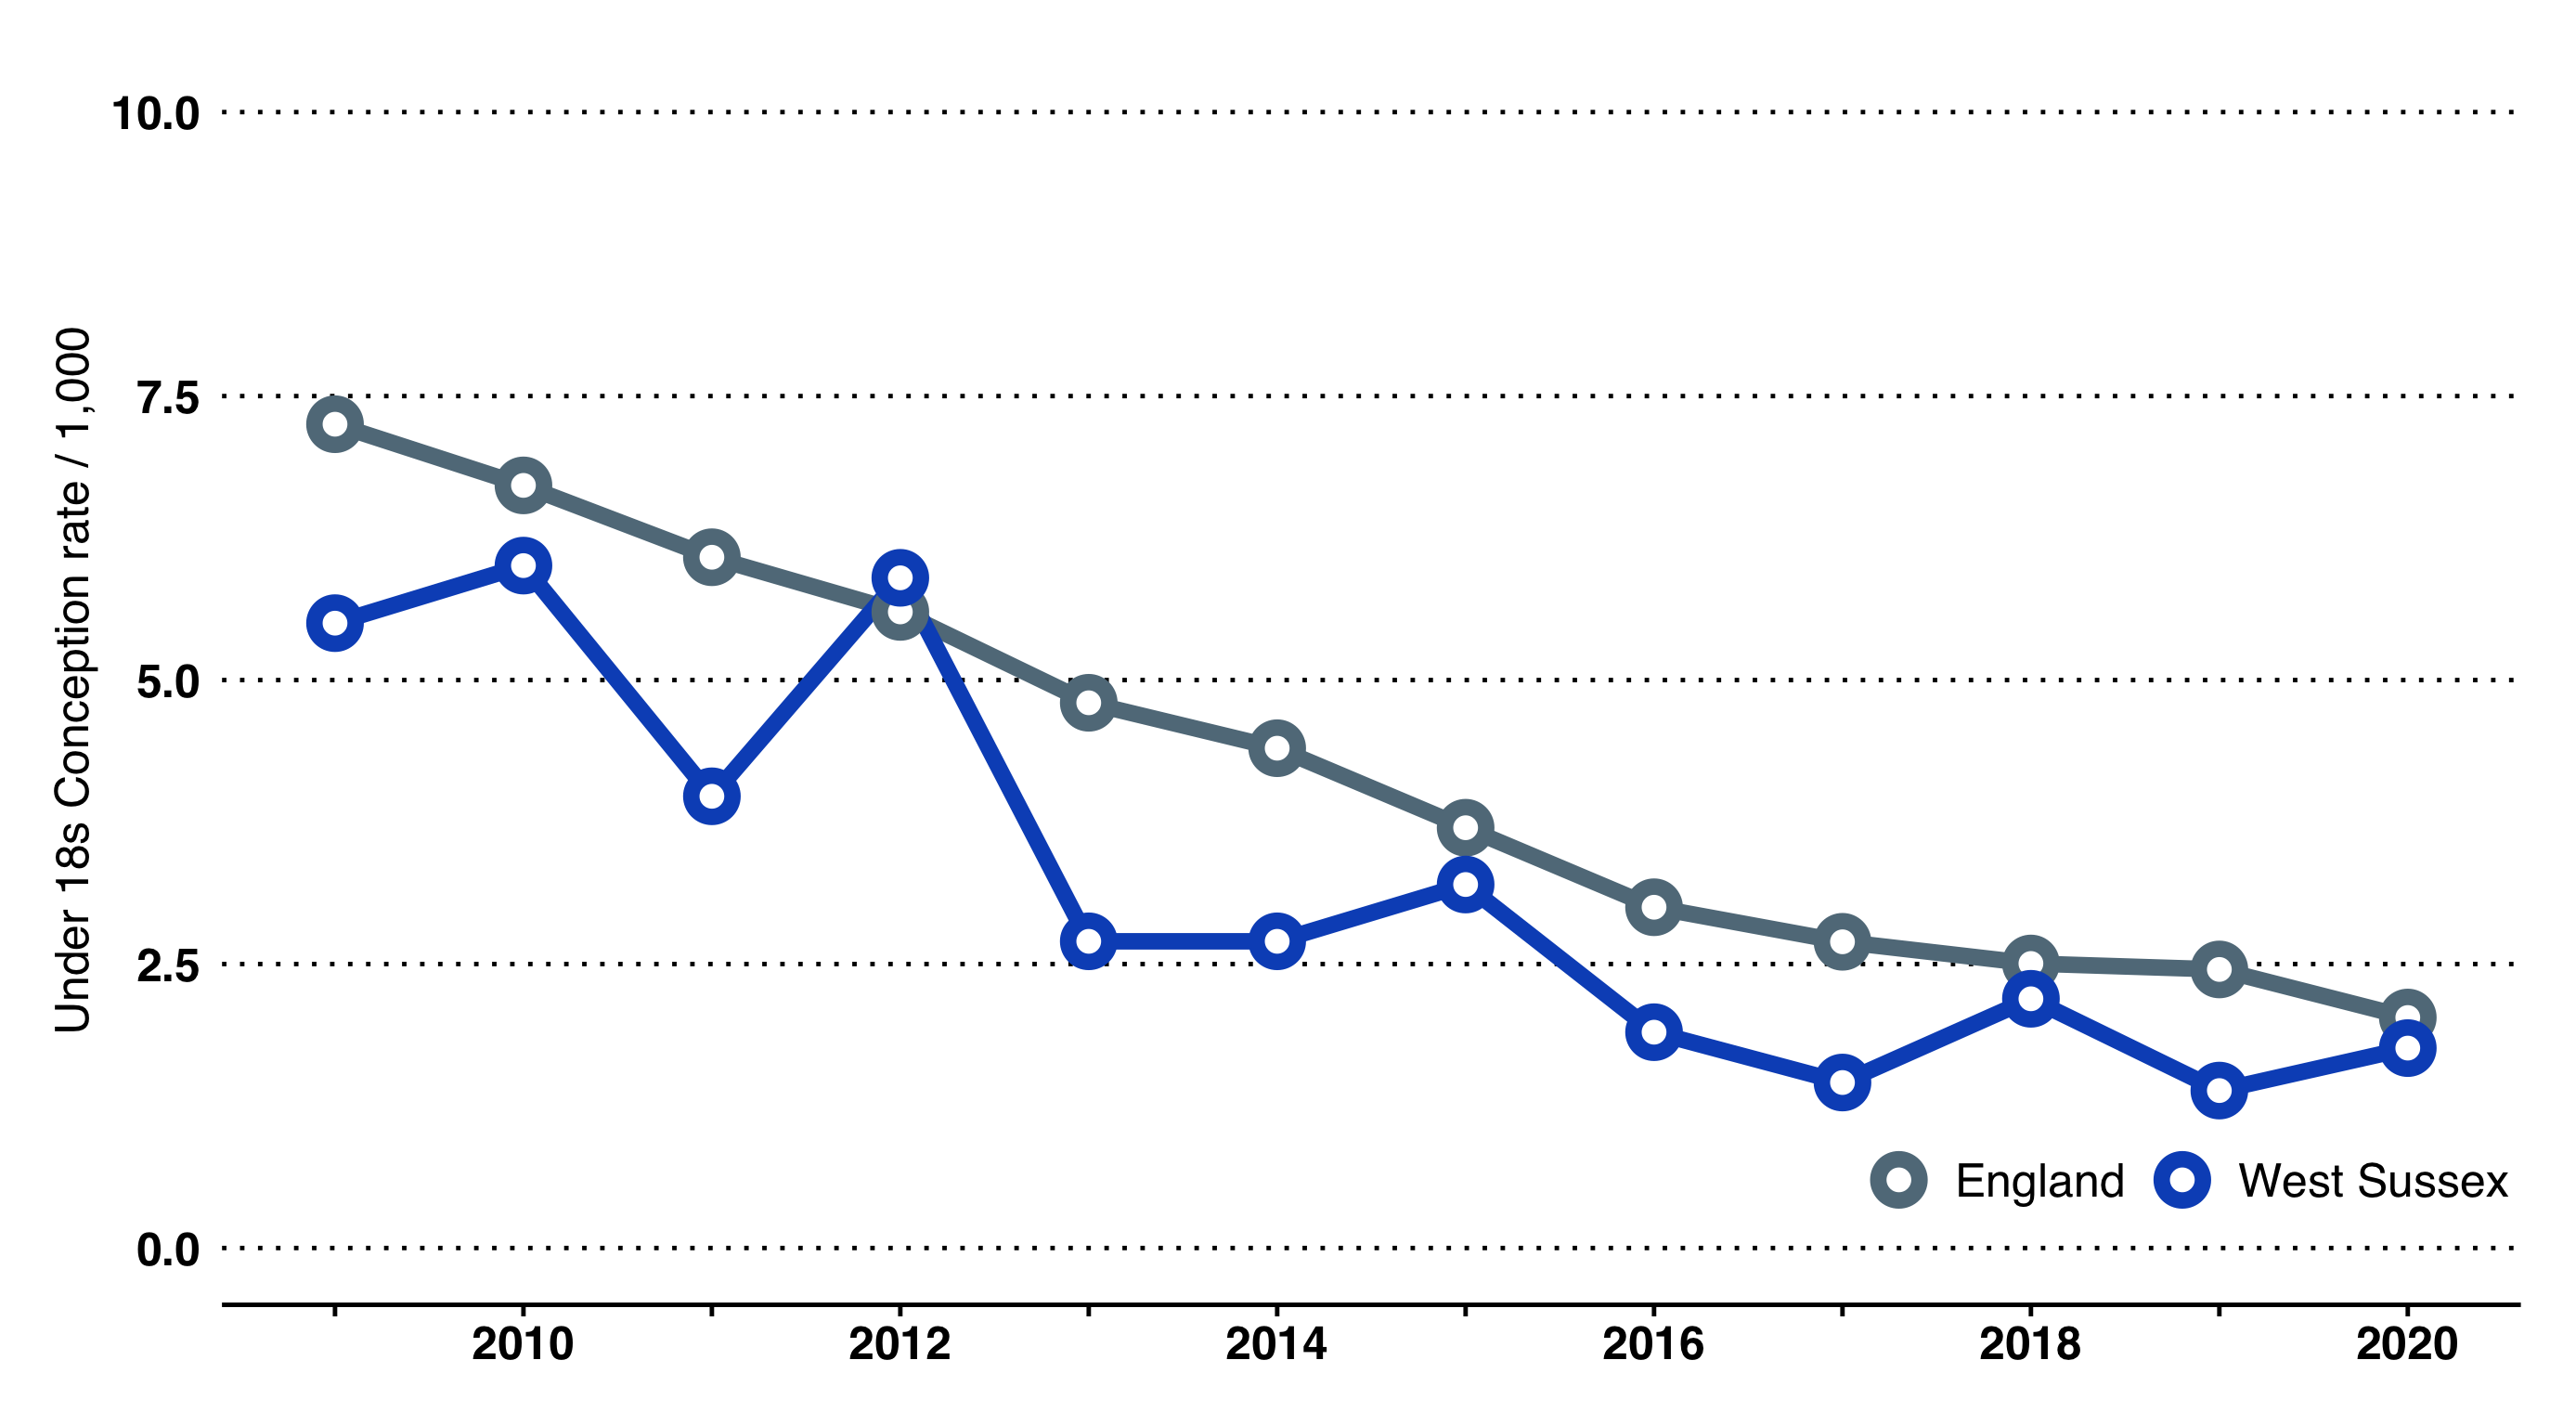
\includegraphics[width = \linewidth]{images/u18s_conc_line.png}
\end{figure}

\begin{figure}[ht]
    \caption{The percentage of abortions undertaken in under 10 weeks has declined in recent years; after a steep fall in 2017, the percentage has risen again, and is now similar to England.}\label{fig:ab_u10wks}
    \centering
    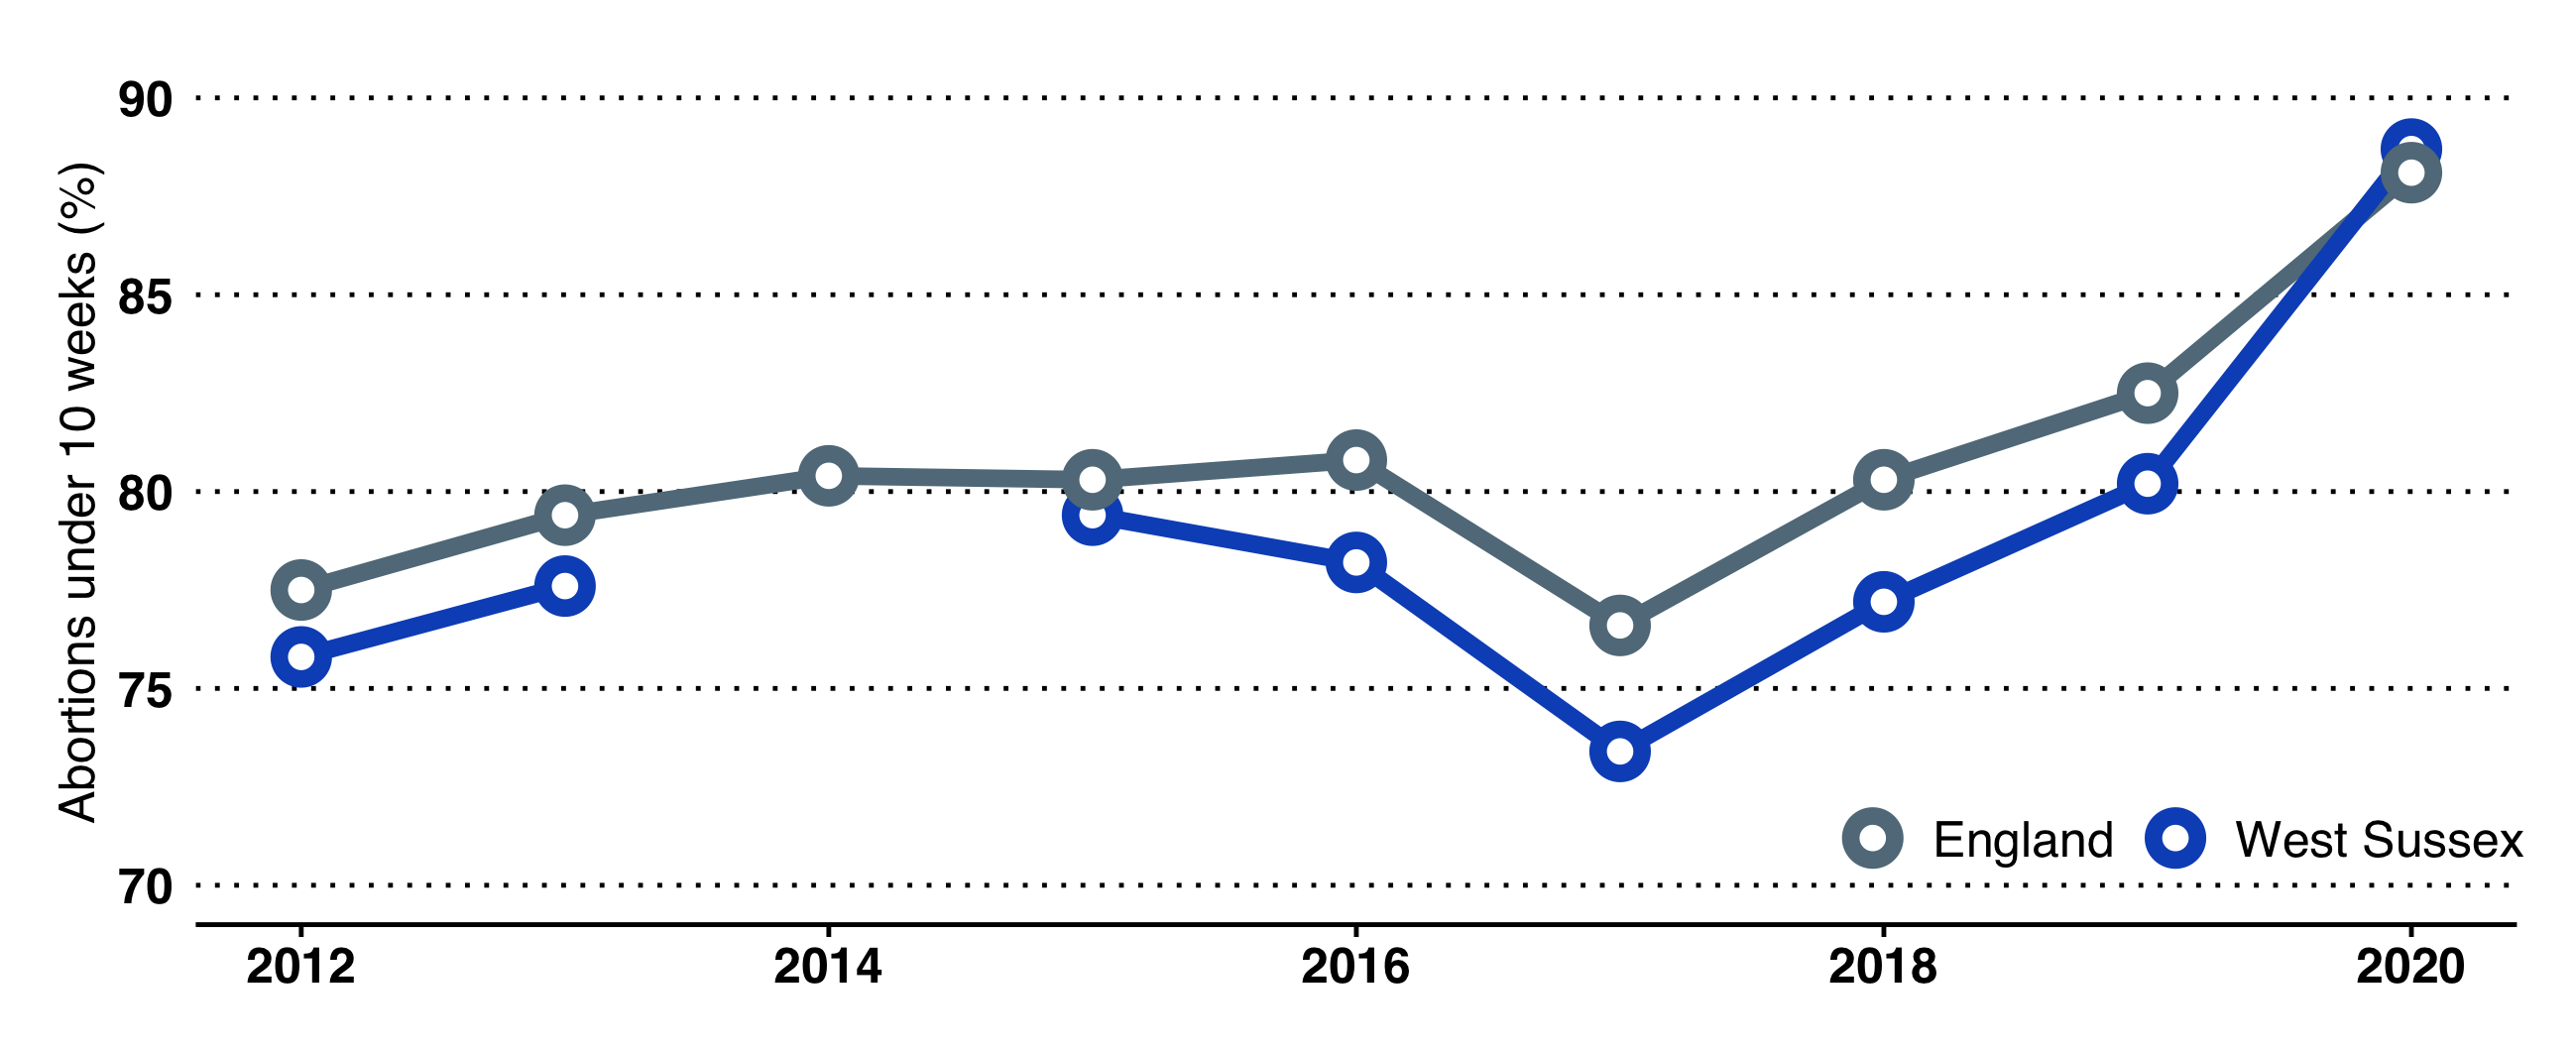
\includegraphics[width = \linewidth]{images/abortions_lt_10wks_line.png}
\end{figure}

\begin{figure}[H]
    \caption{After peaking in 2016, the percentage of repeat abortions in under-25s has fallen to the average level of previous years (around 24\%).}\label{fig:repeat_ab}
    \centering
    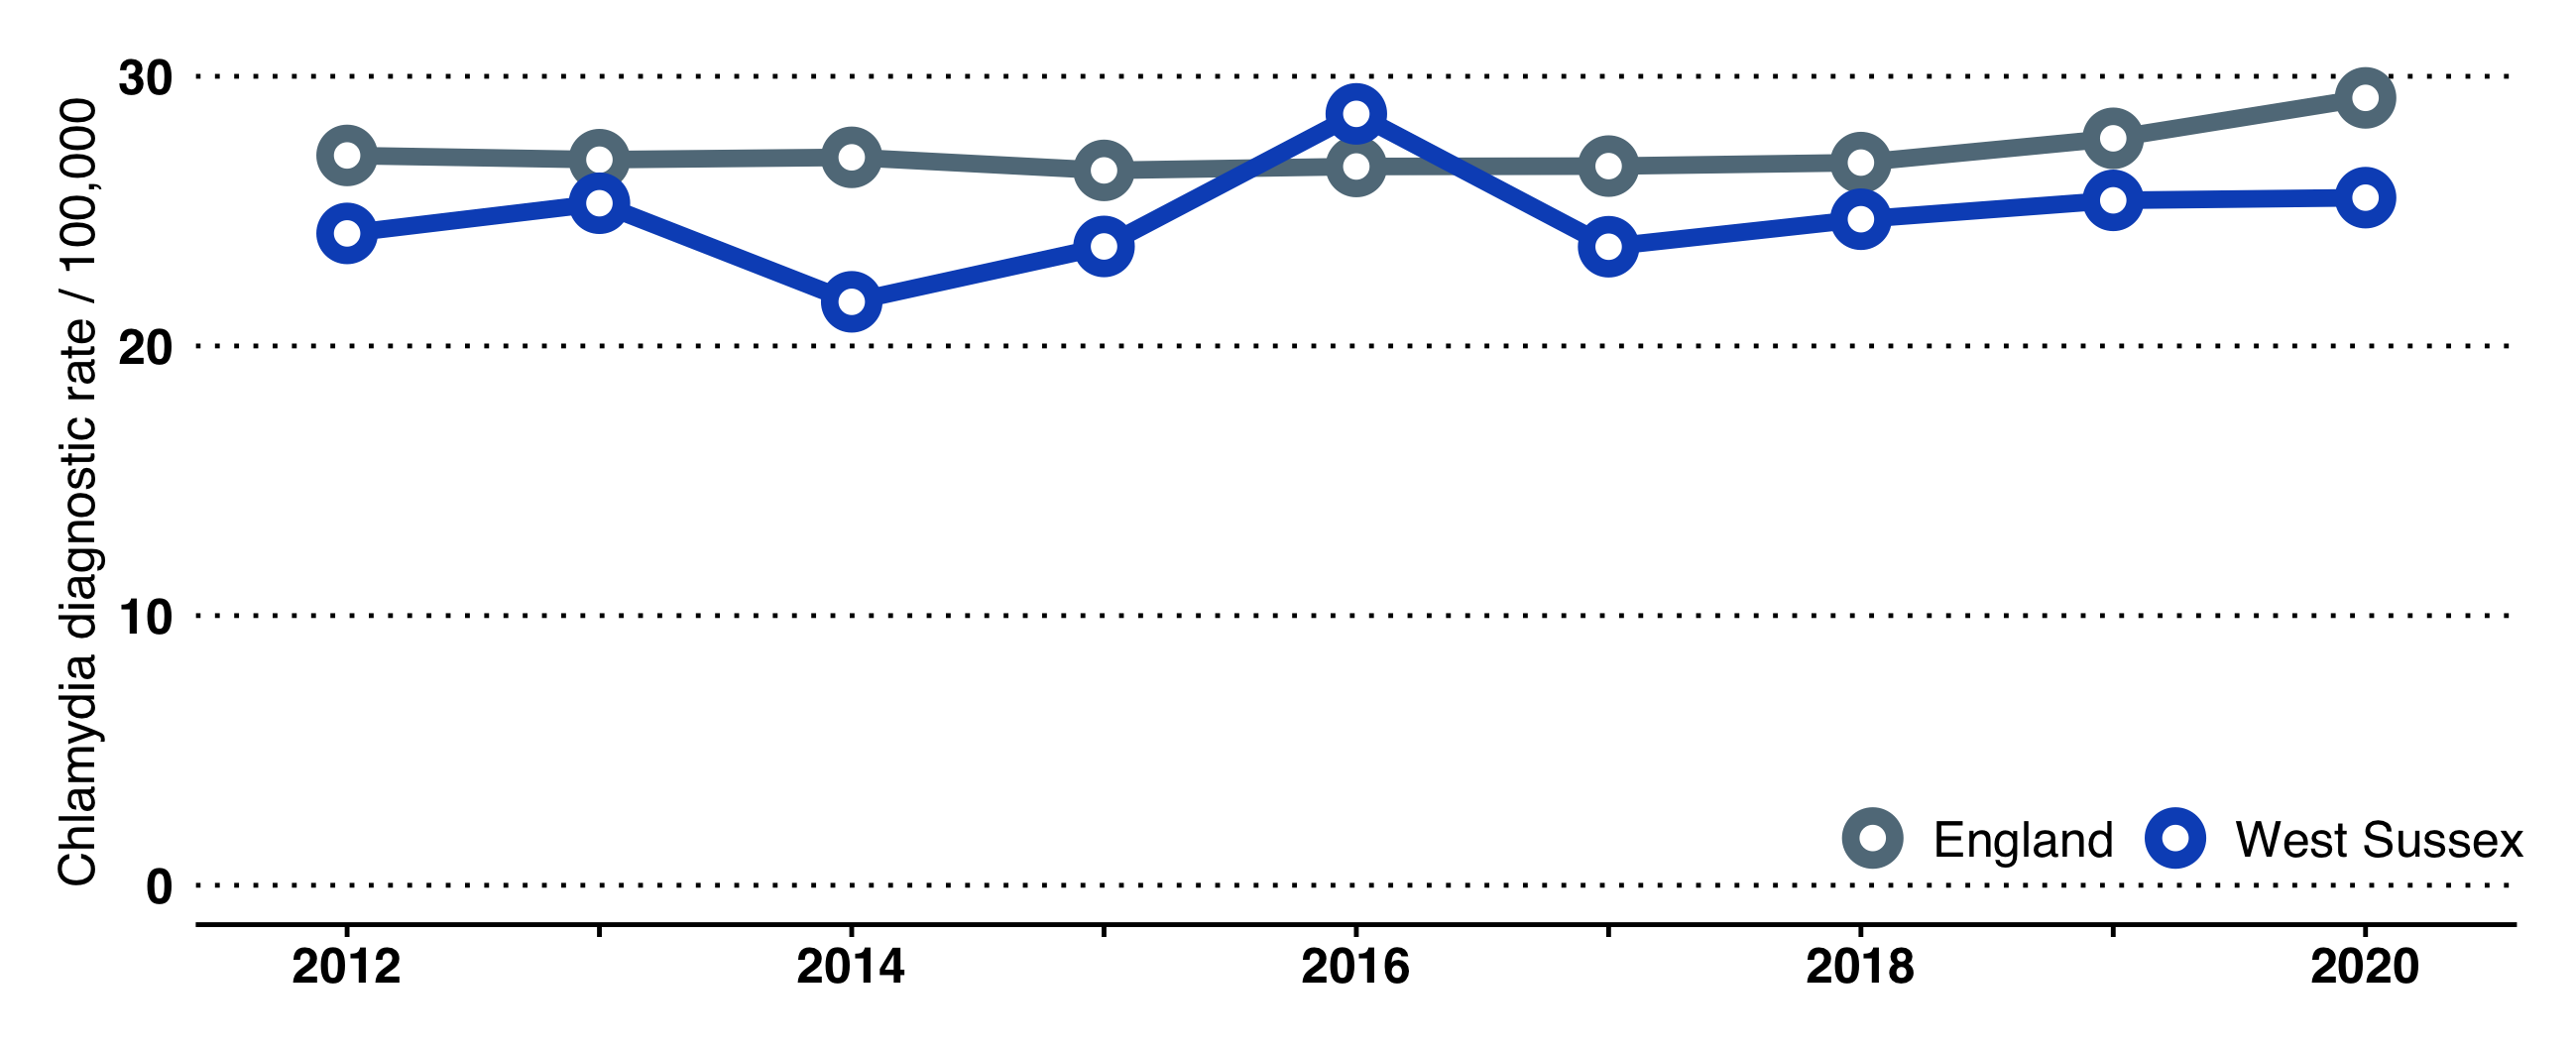
\includegraphics[width = \linewidth]{images/repeat_abortions_line.png}
\end{figure}

\paragraph{A focus on chlamydia} Chlamydia is the most common bacterial sexually transmitted infection in England and causes avoidable sexual and reproductive ill-health. Chlamydia rates are substantially higher in young adults (<25 years) than any other age group, although >25s are also at risk. 

\begin{figure}[ht]
    \caption{West Sussex Chlamydia diagnosis rate. Diagnosis rates have been been falling in West Sussex, even as rates rose in England prior to 2020.}\label{fig:ct_diagnosis}
    \centering
    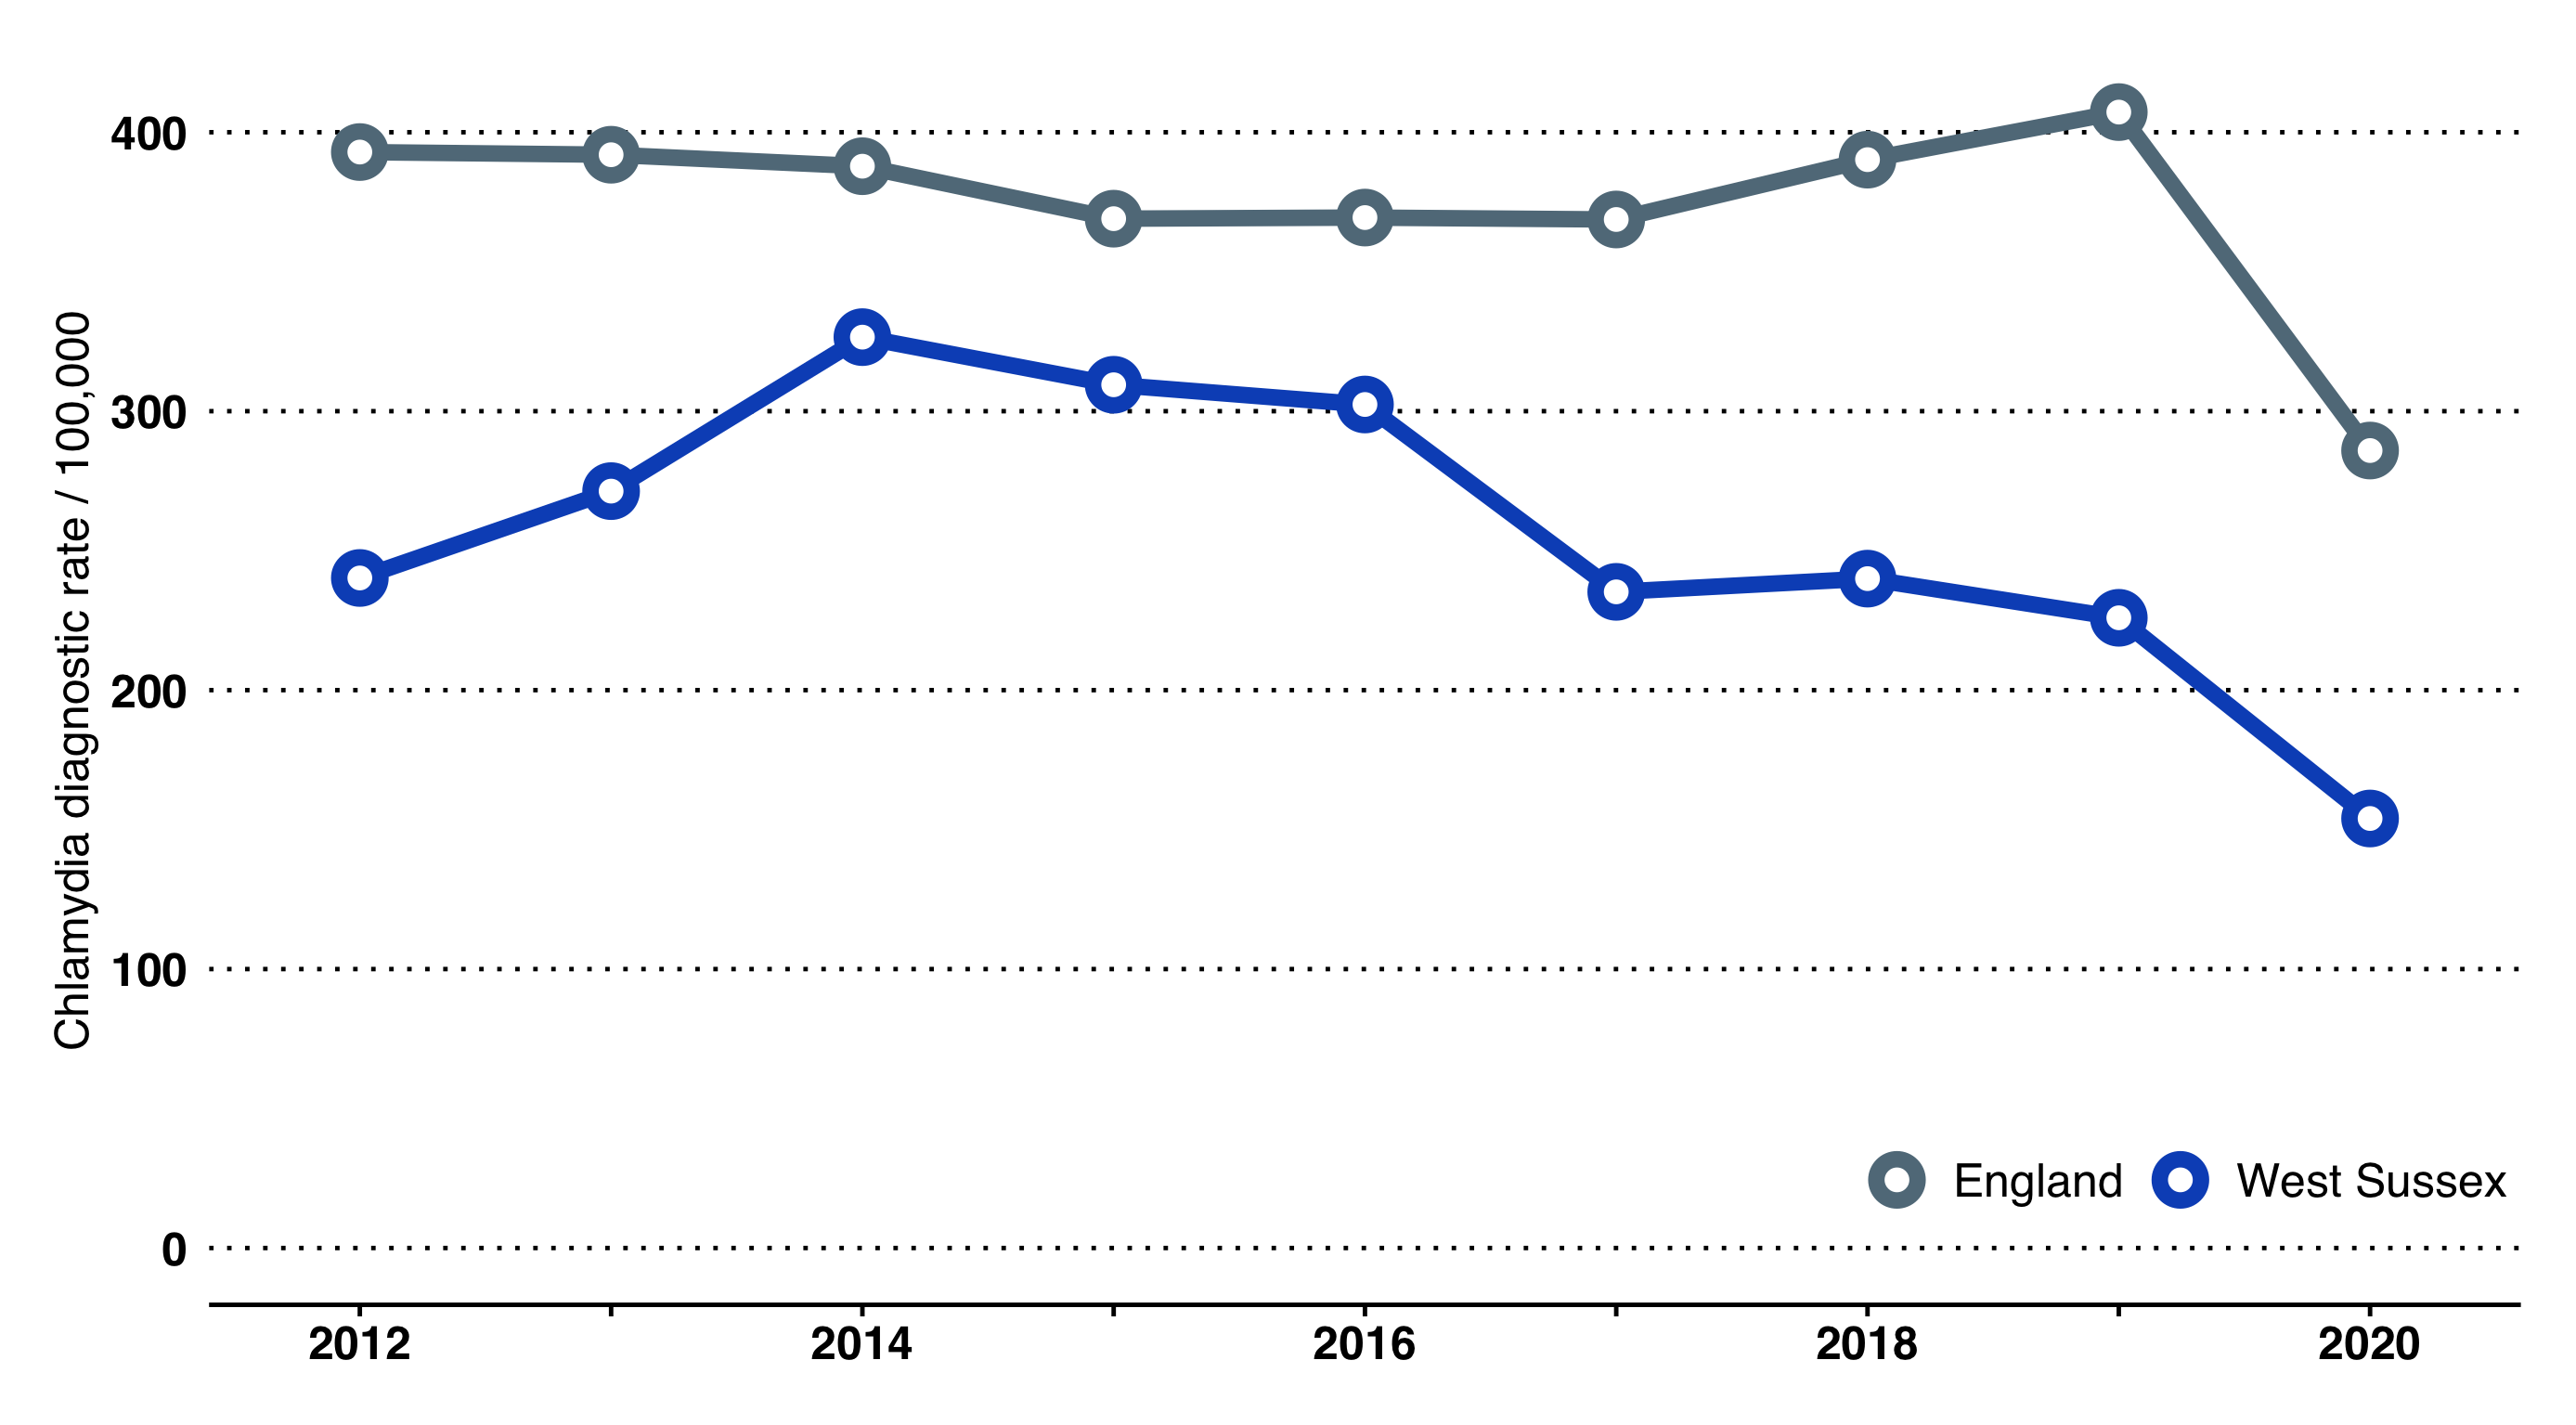
\includegraphics[width = \linewidth]{images/ct_diag_line.png}
\end{figure}

\paragraph{Screening in 15-24 year-olds} Chlamydia screening in 15-24 year-olds allows diagnosis and prompt treatment of symptomatic chlamydia infections. In addition to reducing the time in which the infection can be passed on and thus the spread of chlamydia, screening reduces the chances of an infected individual developing complications.

Screening has declined in West Sussex since 2014 and remains significantly below England in most districts and boroughs, save for Crawley which at 33.3\% of the 15-24 year-old population is signifcantly above the England average (14.3\%) and the highest proportion screened in the South East.

\begin{figure}
    \caption{Percentage chlamydia screening over time and in West Sussex Local Authorities.}
    \label{figure:ct_screen_wsx}
    \centering
    \begin{subfigure}[b]{0.99\linewidth}
        \centering
        \caption{Annual percentage of 15-24 year olds screened  for Chlamydia, West Sussex 2012 to 2020.}\label{fig:chlamydia:p_u25_time}
        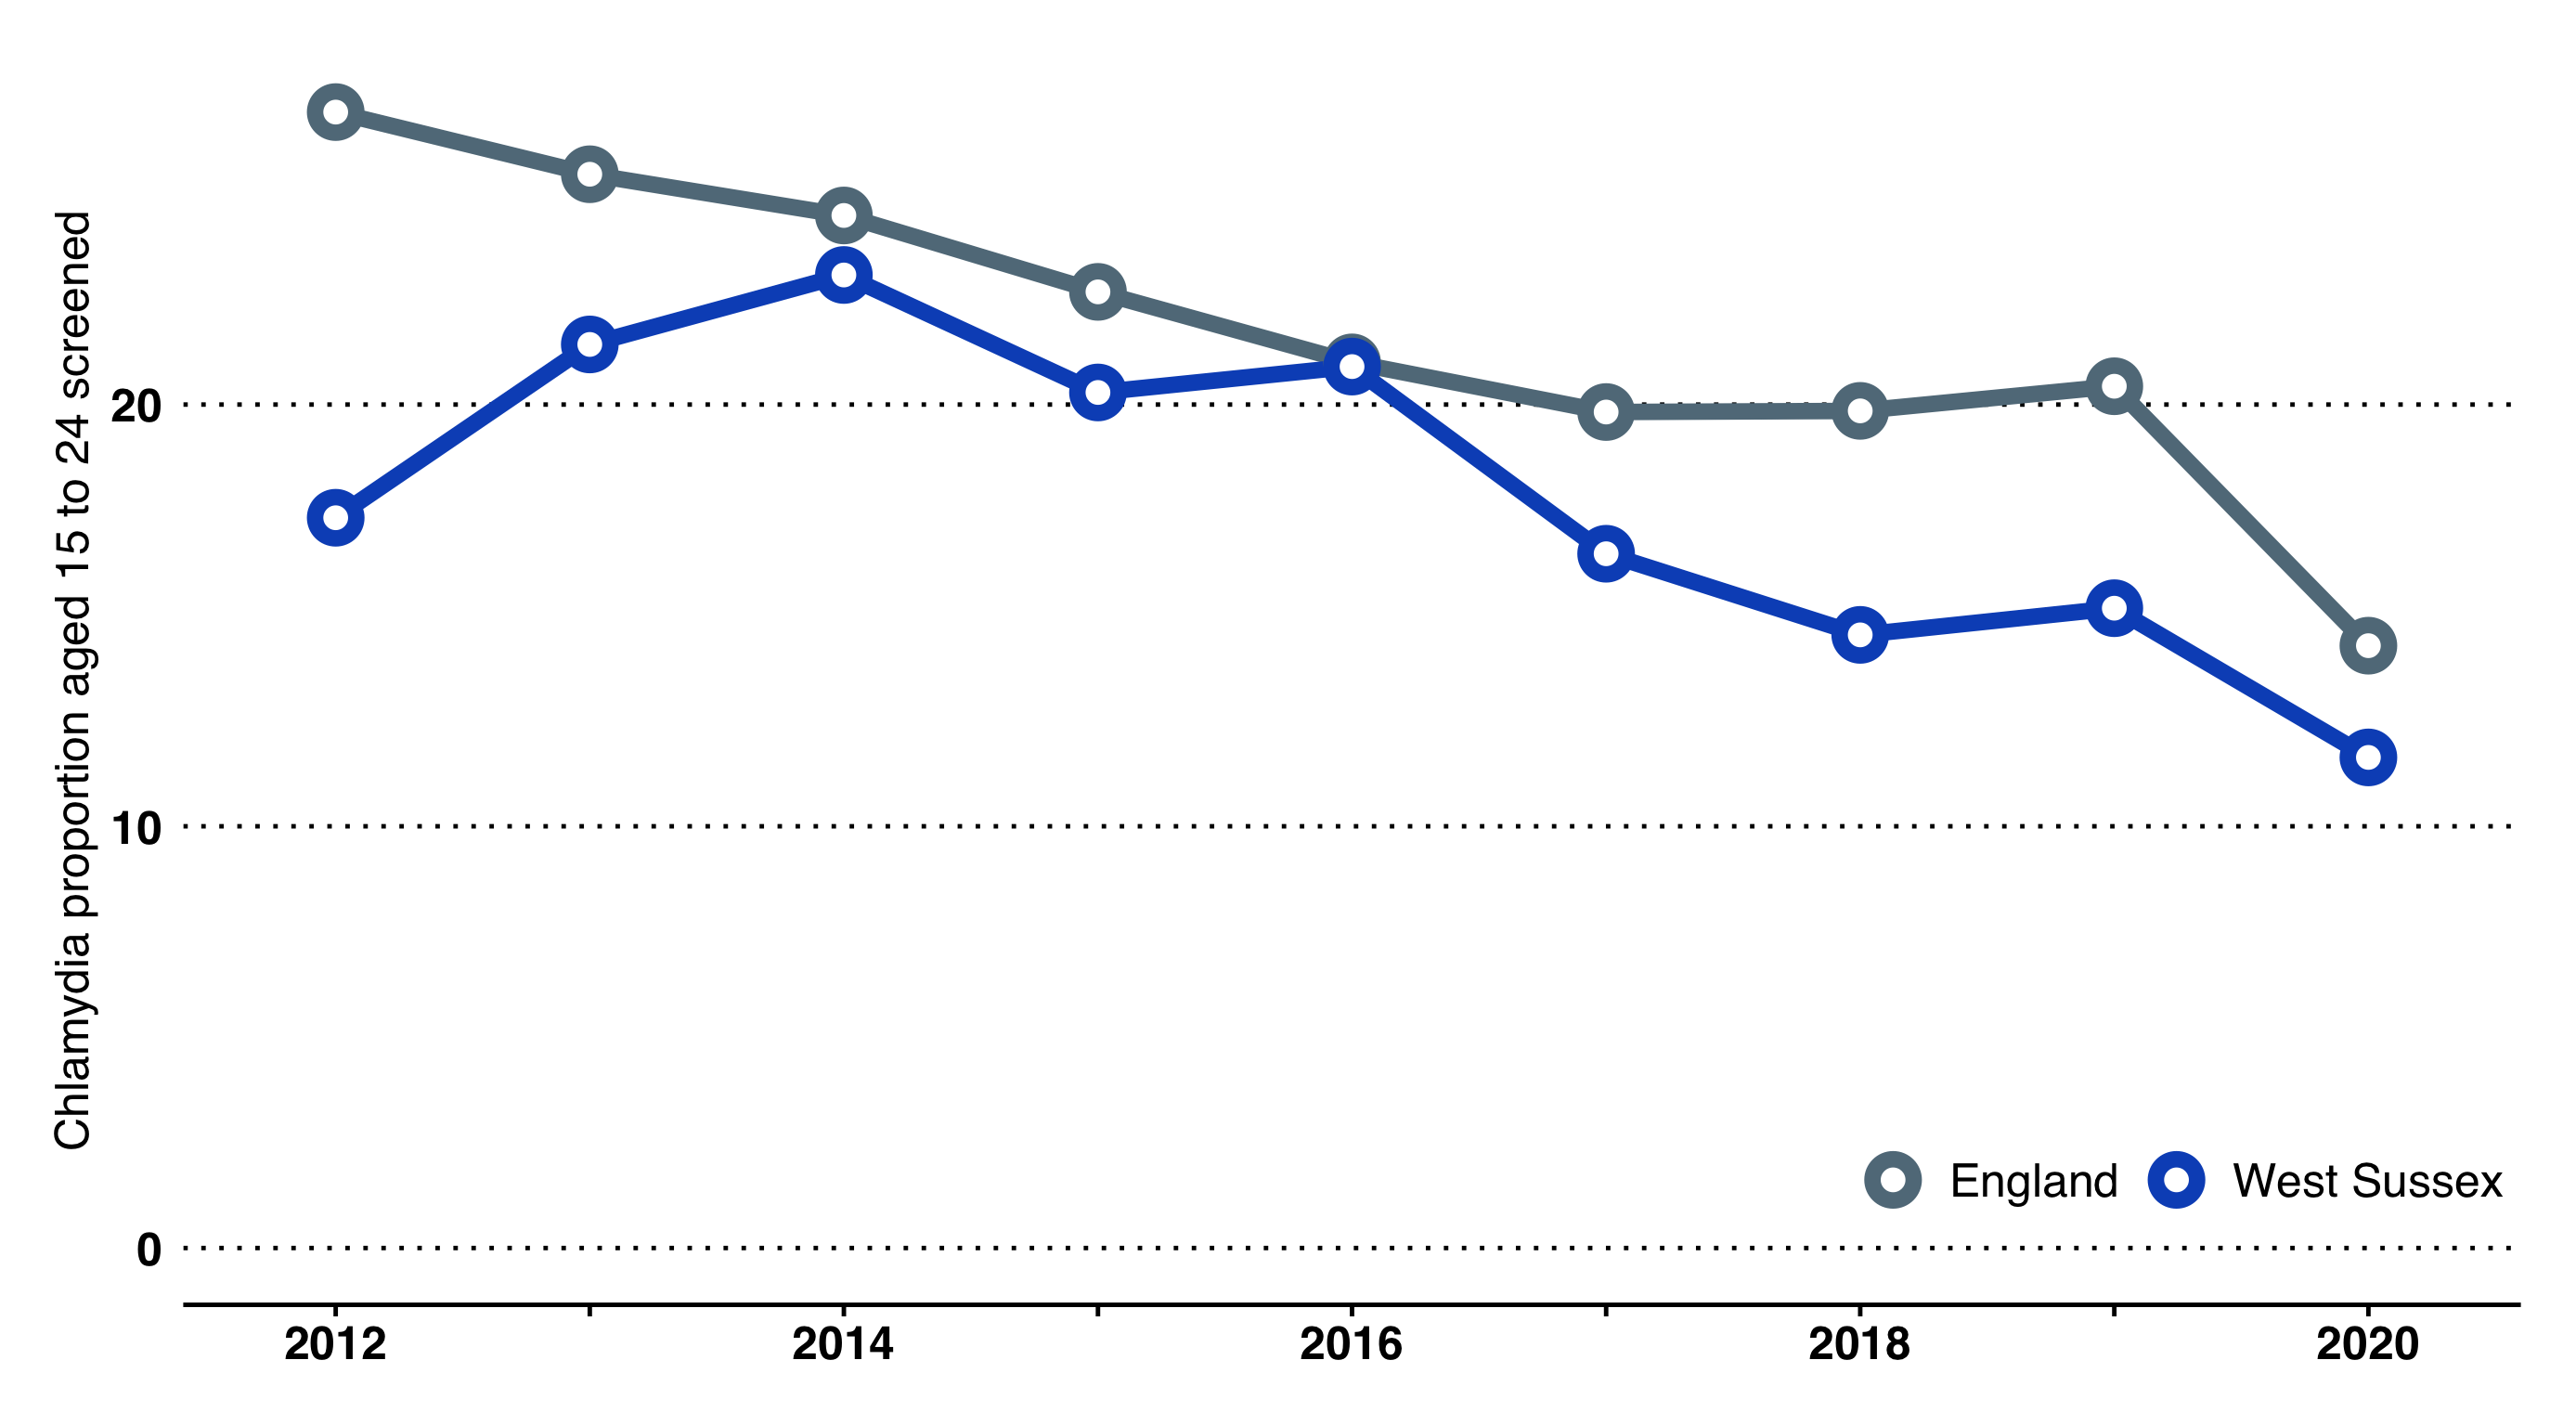
\includegraphics[width=\linewidth]{images/ct_screened_line.png}
    \end{subfigure}
    \begin{subfigure}[b]{0.99\linewidth}
        \centering
        \caption{Percentage of 15-24 year olds screened for Chlamydia, West Sussex Local Authorities 2020.}\label{fig:chlamydia:p_u25_dabs}        
        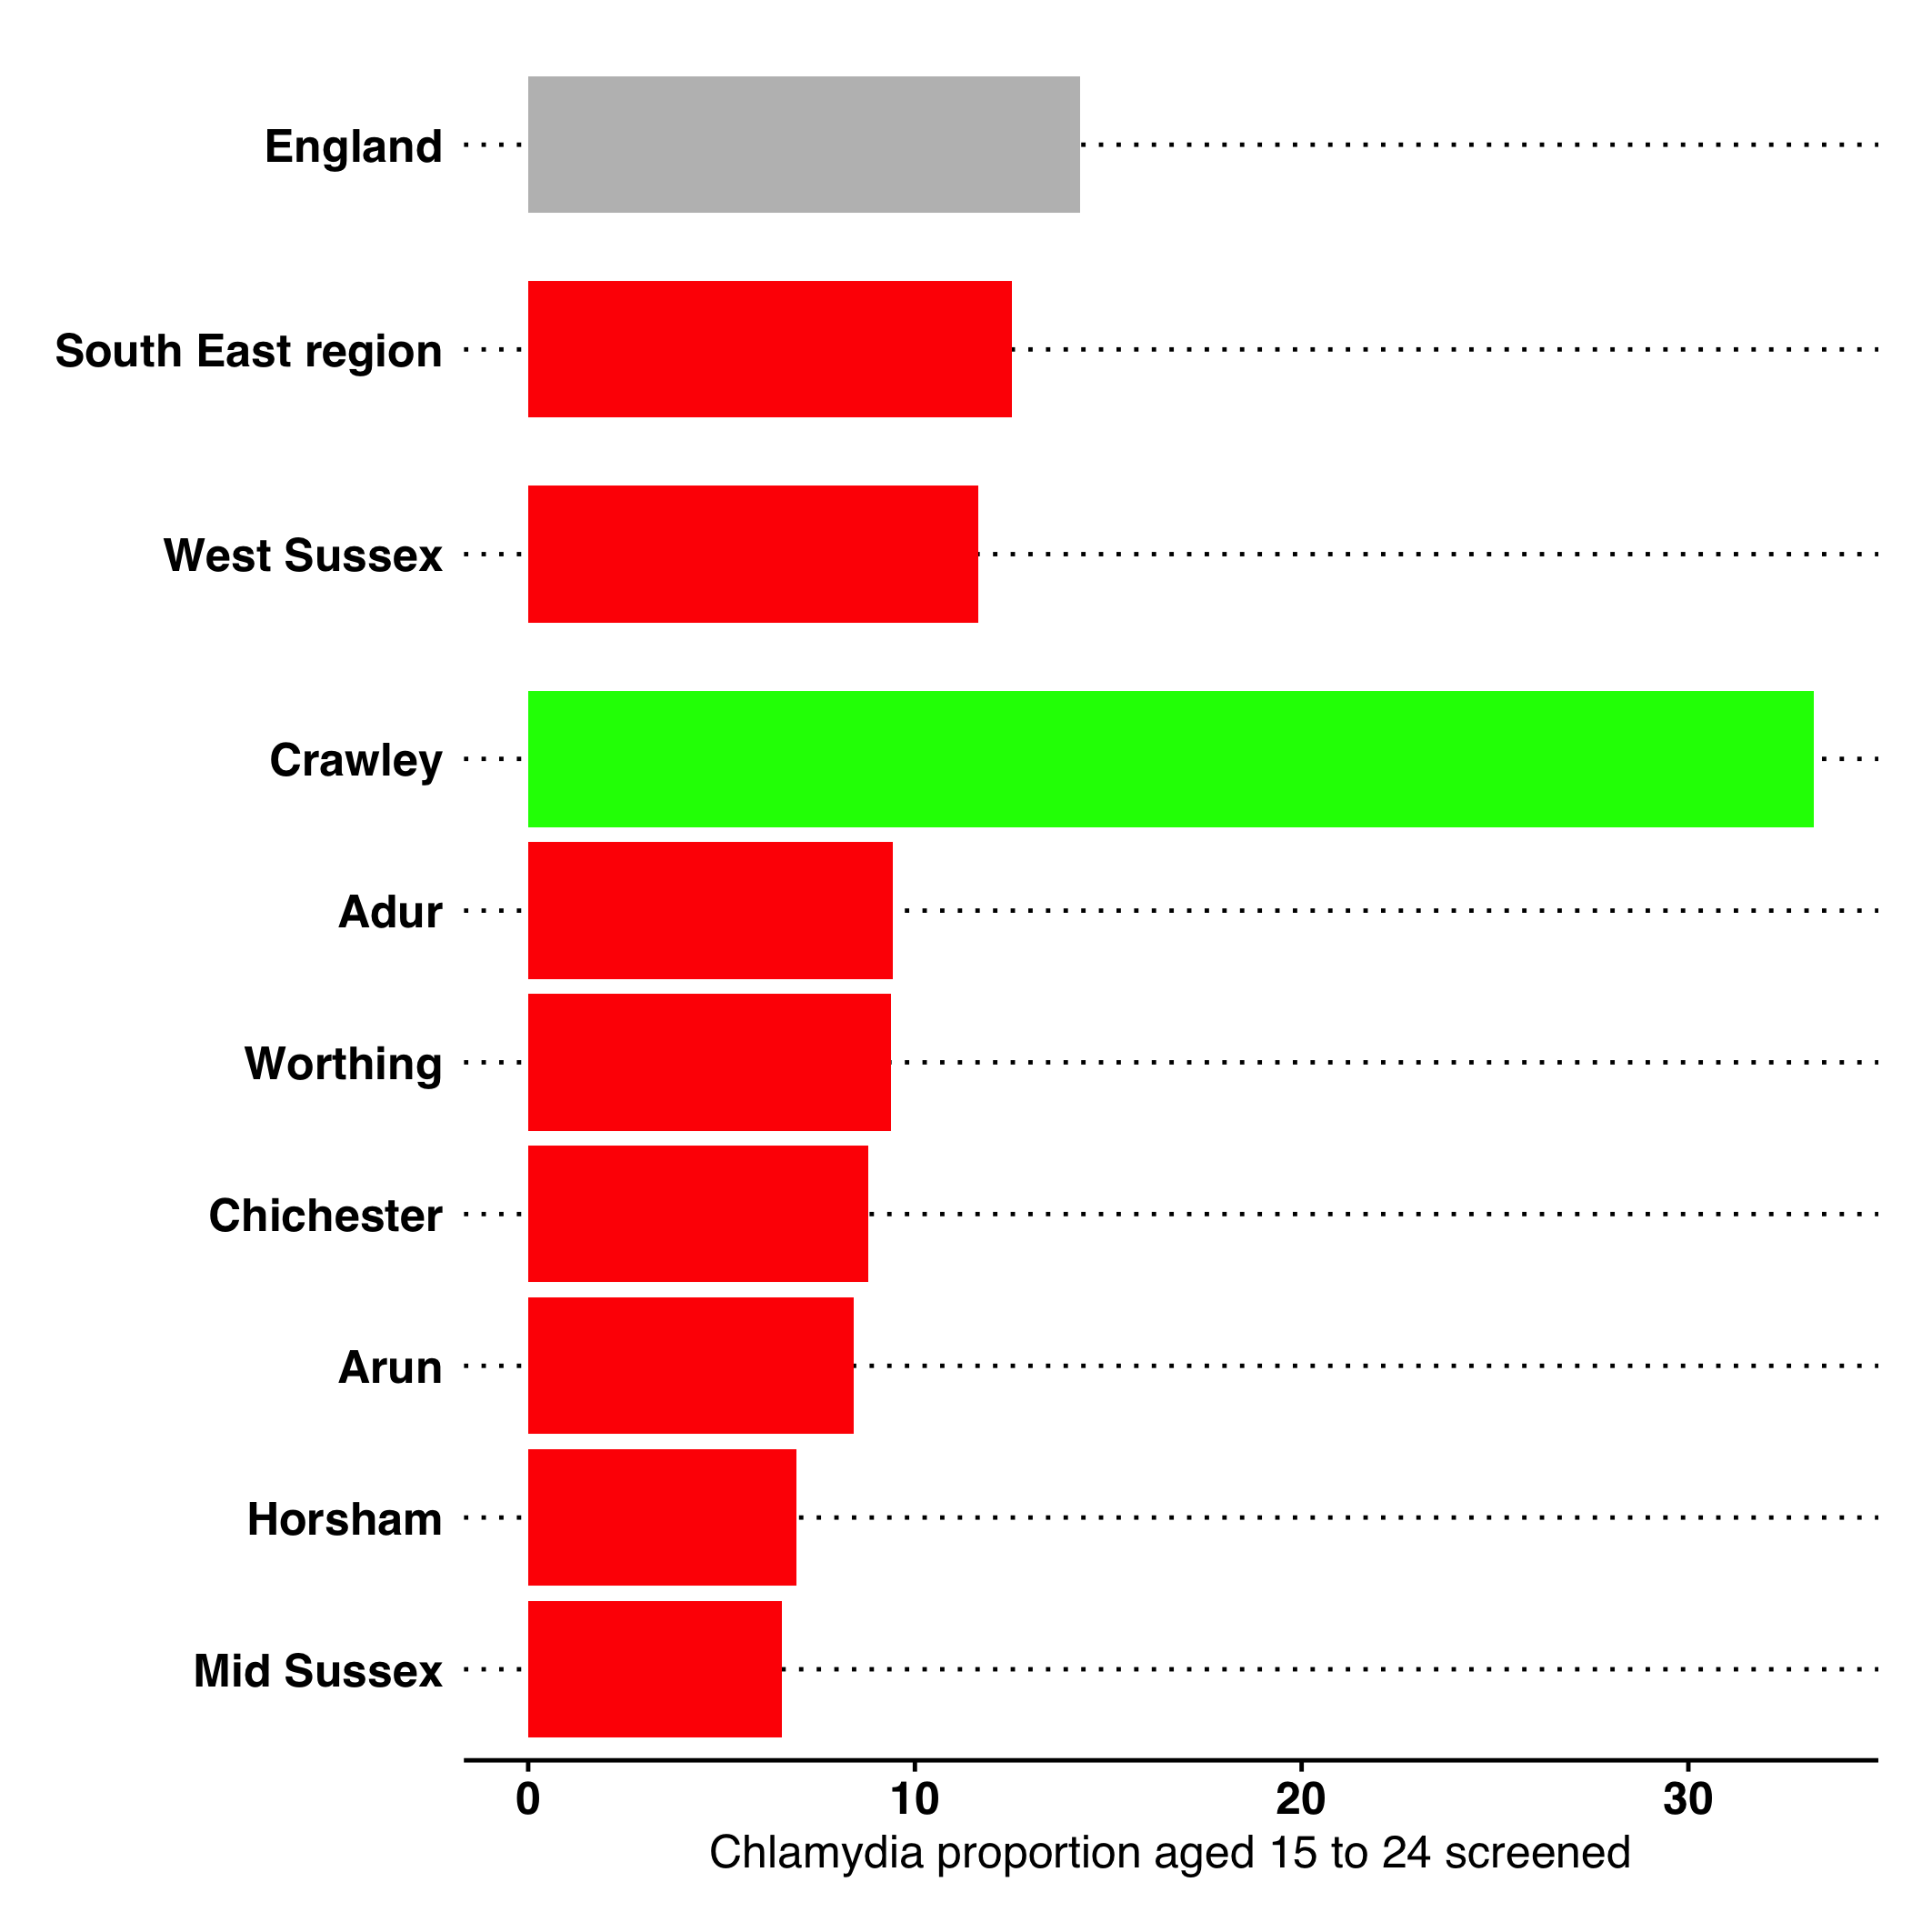
\includegraphics[width=\linewidth]{images/chlamydia_screen_yp_rag_bar.png}
    \end{subfigure}
    \vspace*{3mm}
\end{figure}



%\subsection{A Focus on HEALTH PROTECTION} 
%The West Sussex Health Protection Annual Report 2018/19 details the state of efforts to prevent and reduce ill-health in West Sussex, many of which are measures in the Public Health Outcomes Framework. This report is available on the JSNA website. For further information, contact Lobat Salehi (\url{lobat.salehi@westsussex.gov.uk}).

%\paragraph{Outbreaks}There were 246 outbreak situations or incidents in 2018/2019. Specific cases and outbreaks of note include:

%\begin{itemize}
%    \item a number of complex TB cases and incidents requiring place-based screening of contacts, including exposures in hospitals, schools and immigration removal centres.
%    \item outbreaks of seasonal flu in hospitals and care homes. GP Influenza-like illness (ILI) consultation rates peaked later in the 2018/19 season in West Sussex, at 23.4 per 100,000, than the South East and England and were lower than in the 2017/18 season.
%    \item a large Cryptosporidium outbreak relating to visits to an open farm in West Sussex during lambing season (one of four Cryptosporidium outbreaks related to open farms during lambing season across the South East in 2018/19), with a multi -agency response to investigate and manage the public health risk. 203 cases with a known link to the farm were recorded (119 confirmed, 82 probable and 2 possible).
%    \item a measles outbreak in school pupils in the Chichester area, with 29 reported cases (22 confirmed, 4 probable, 3 possible). Additional MMR vaccination catch-up clinics were offered for unvaccinated children in the area.
%\end{itemize}
   
%\subsubsection{Key challenges outlined in the 2018/19 annual report} In West Sussex, key challenges around infectious diseases are:

%\begin{itemize}
%    \item the large numbers of care homes, settings which are at risk of flu and norovirus outbreaks. Alongside the consequential impacts on the wider health economy and individuals within the care system from these outbreaks, care homes are often noted to have no or poorly effective occupational health services, resulting in low flu vaccination uptake rates for their staff 
%    \item prison and detention settings tend to out-source occupational health provision, which can often lead to delays in provision of public health measures on-site for staff, thus impacting on rapid responses to contain outbreaks
%    \item the on-going resourcing pressures on environmental health teams who enforce health protection legislation and implement controls during outbreaks, causing potential delays to managing gastro-intestinal cases and outbreaks
%    \item uptake of the two MMR vaccines by 5 years olds not reaching the 95\% target required to provide adequate herd immunity\footnote{PHOF reference D04c}, increasing the risk of widespread measles outbreaks
%    \item increasing numbers of open farms providing open days to the public during lambing season. Awareness of the required standards documented in the Industry Code of Practice is needed to reduce the risk of the spread of gastrointestinal illness
%    \item higher rates of TB in the Crawley area compared with the South-East and England rates (See Table~\ref{tab:wa:tb} on page~\pageref{tab:wa:tb}).
%\end{itemize}

%\begin{table}
%    \caption{TB Rates (per 100,000 population)}
%    \centering
%    \begin{tabular}{llll}
%    \toprule
%    \ & Crawley & South East & England \\
%    \midrule
%    2017 & 12.5 & 6.2 & 9.1 \\
%    2016 & 20.6 & 6.5 & 10.1 \\
%    \bottomrule
%    \end{tabular}
%    \label{tab:wa:tb}
%\end{table}

\subsection{Screening}
\subsubsection{Flu jabs - for at risk groups} Coverage of flu vaccinations for at-risk groups\footnote{PHOF reference D05. These are individuals from age six months to under 65 years, excluding otherwise 'healthy' pregnant women and carers.} was 56.7\% in 2020/21. Coverage has been increasing year on year since 2015/16, remains above the England rate and is now above the $\geq$55\% benchmark.

\begin{figure}[htp]
    \caption{Flu vaccination coverage - at risk groups, West Sussex, 2010/11 to 2020/21.}
    \centering
    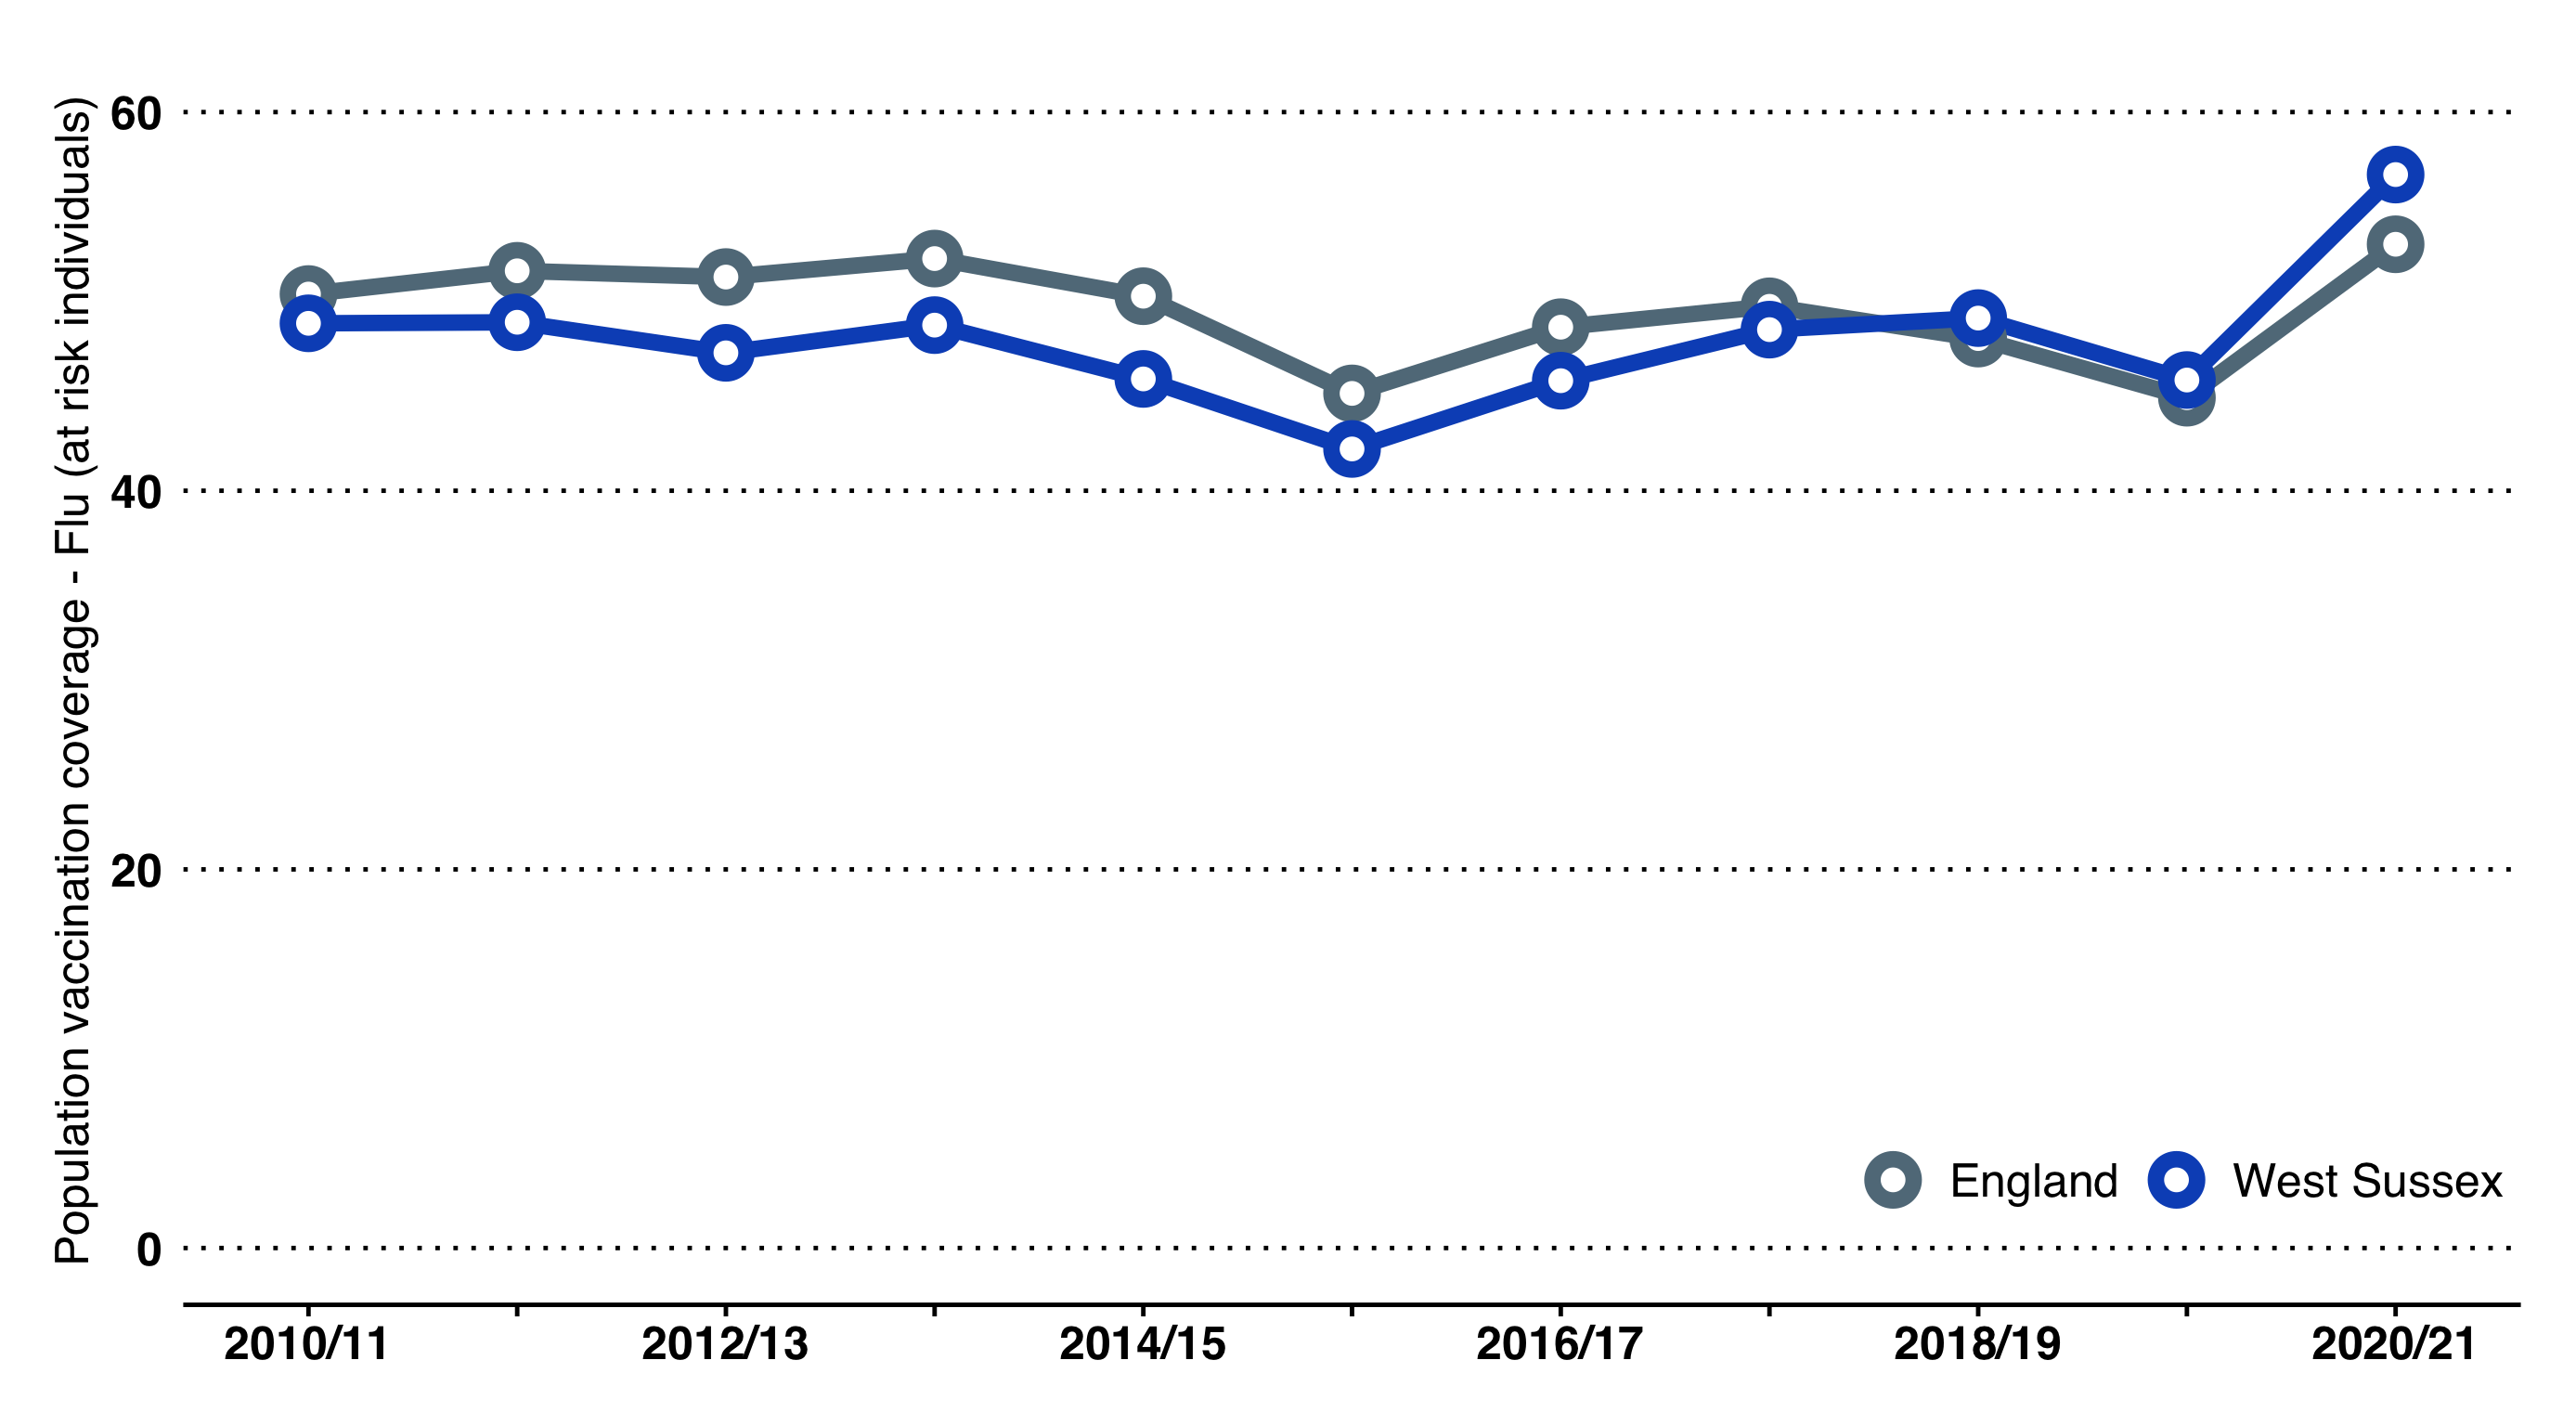
\includegraphics[width=\linewidth]{images/flu_vax_at_risk_popn.png}
    \label{fig:flu_vax_at_risk_coverage}
\end{figure}

Flu vaccinations for frontline healthcare workers involved in direct patient care increased nationally from 2017/18 to 2018/19, although there is variation above and below the 75\% target between the NHS Foundation Trusts serving the population of West Sussex.\footnote{Note: These figures have not been updated since 2018/19.}

\subsubsection{NHS Health Checks} For NHS Health Checks, West Sussex continues to perform poorly compared with England on all outcome measures\footnote{PHOF references C26a, C26b and C26c}:

\begin{itemize}[noitemsep]
    \item The cumulative percentage of the eligible population aged 40-74 offered an NHS Health Check in the five year period 2016/17 - 2020/21 was 60.4\%.
    \item The cumulative percentage of the eligible population aged 40-74 offered an NHS Health Check who received an NHS Health Check in the five year period 2016/17 - 2020/21 was 35.2\%, a decrease on the previous five year period.
    \item The cumulative percentage of the eligible population aged 40-74 who received an NHS Health Check in the five year period 2014/15 - 2018/19 was 21.3\%.
\end{itemize}


\subsubsection{Non-Cancer Screening}
\paragraph{Abdominal Aortic Aneurysm screening coverage} The screening coverage rate at county-level for abdominal aortic aneurysm (PHOF reference C25a) was 76.7\% in 2020/21, compared to 55.0\% in England overall. Coverage in all West Sussex local authorities is higher than the South East and England.
% Have removed the plot of coverage over time as figures are a little wild.
\begin{figure}[ht]
    \caption{Abdominal Aortic Aneurysm screening coverage, West Sussex local authorities, 2020/21.}
    \label{figure:aaa:screening}
    \centering
    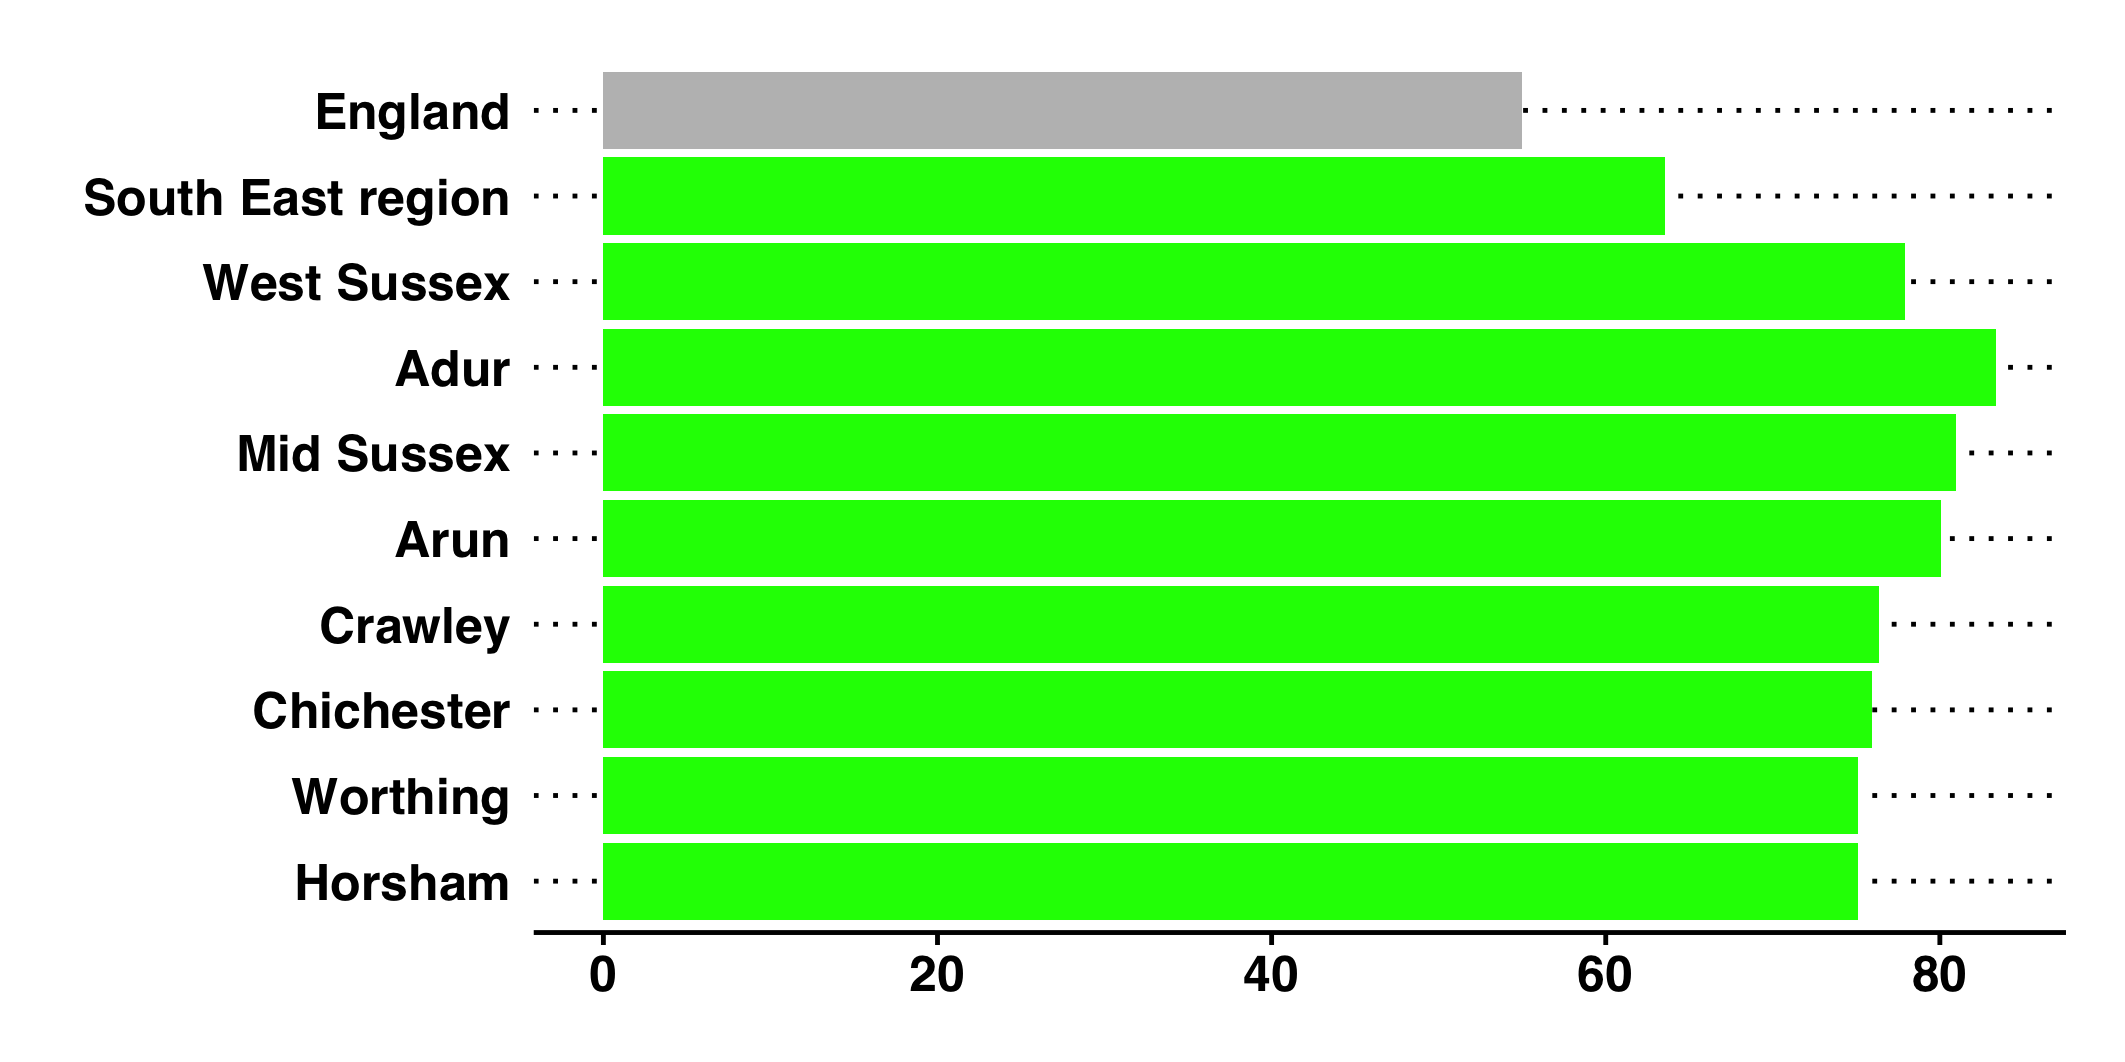
\includegraphics[width=\linewidth]{images/aaa_rag_bar.png}
\end{figure}

\paragraph{Diabetic Eye screening uptake}At the time of writing, only regional figures were available for the uptake of routine digital screening events for diabetic eye\footnote{PHOF reference C25b}. In the south east uptake was 79.2\% in 2020/21, comparing favourably to the England rate.

However this figure is lower than past coverage in West Sussex (e.g. 87.5\% uptake rate in 2018/19), indicating the disruptive effect of the pandemic on preventative screening efforts.



\subsubsection{Cancer Screening Programmes}
At county-level, overall take-up rates of screening programmes are good, comparing favourably with England and in line with rates in statistical neighbours (Figure~\ref{fig:cancer-screening}). However, there is variation between the West Sussex local authorities, with notably low rates in Crawley. All relate to 2020/21\footnote{Cervical cancer screening, PHOF reference C24b. Breast cancer screening, PHOF reference C24a. Bowel cancer screening, PHOF reference C24d.}.

% Might need to go back and make the RAG bar charts a bit taller - will see how it looks in the print out

\begin{figure*}
    % At county-level, overall take-up rates of screening programmes are good, comparing favourably with England and in line with rates in statistical neighbours. However, there is variation between the West Sussex local authorities, with notably low rates in Crawley. All relate to 2020/21.\\
    \caption[Cancer screening rates in West Sussex and its consituent lower tier local authorities.]{The screening rate at county-level for {\bf cervical cancer} (in women aged 25-49 years) is 72.2\% (Crawley, 67.3\%). Uptake had reached a 20-year low in 2018, although promotional campaigns have contributed to increases since. For {\bf breast cancer}, the screening rate at county-level is 73.1\% (Screening rates are higher than England for all districts and boroughs in West Sussex, though rates are lowest in Crawley, 65.0\%). Recent issues with the West Sussex breast programme's round length may explain the decline in screening coverage. The screening rate at county-level for {\bf bowel cancer} is 69.4\% (Crawley, 64.7\%).}\label{fig:cancer-screening}
    \vspace*{5mm}
    \centering
    \begin{subfigure}[b]{0.32\textwidth}
        \centering
        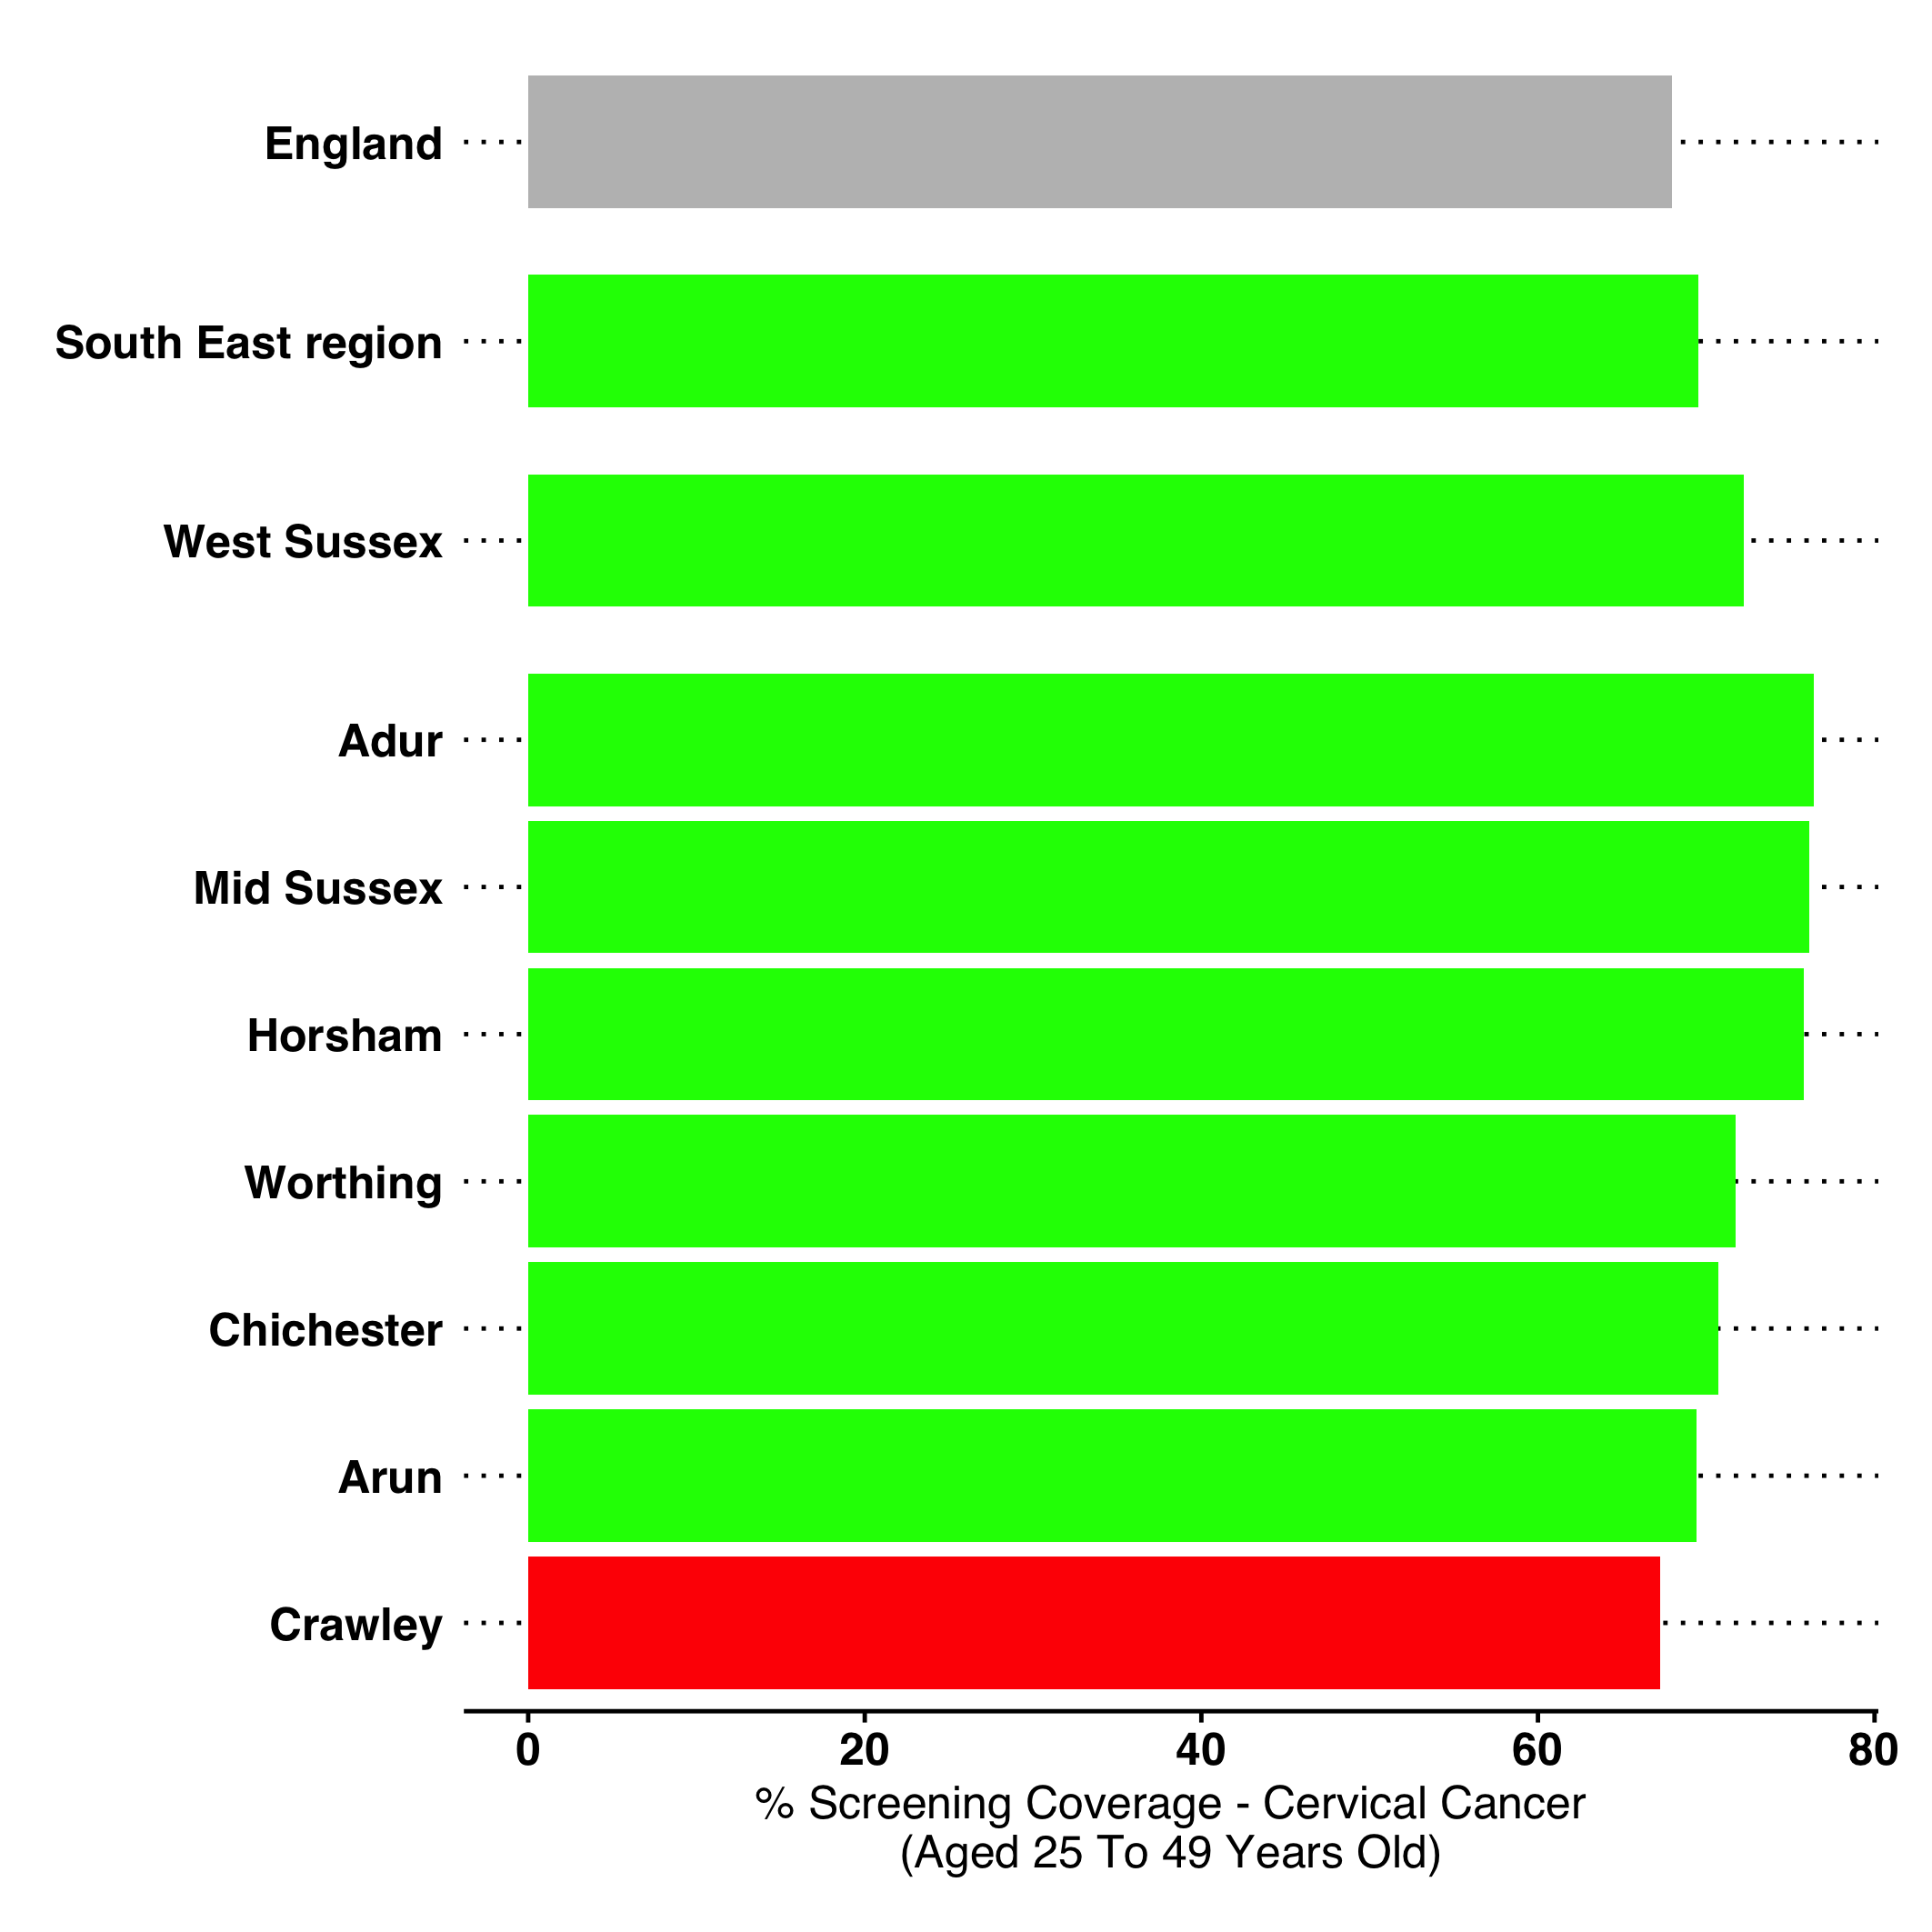
\includegraphics[width=\textwidth]{images/cervical_cancer_rag_bar.png}
        \caption{Cervical cancer screening coverage 2020/21 West Sussex Local Authorities}
        \label{fig:cervical:rag}
    \end{subfigure}
    \begin{subfigure}[b]{0.32\textwidth}
        \centering
        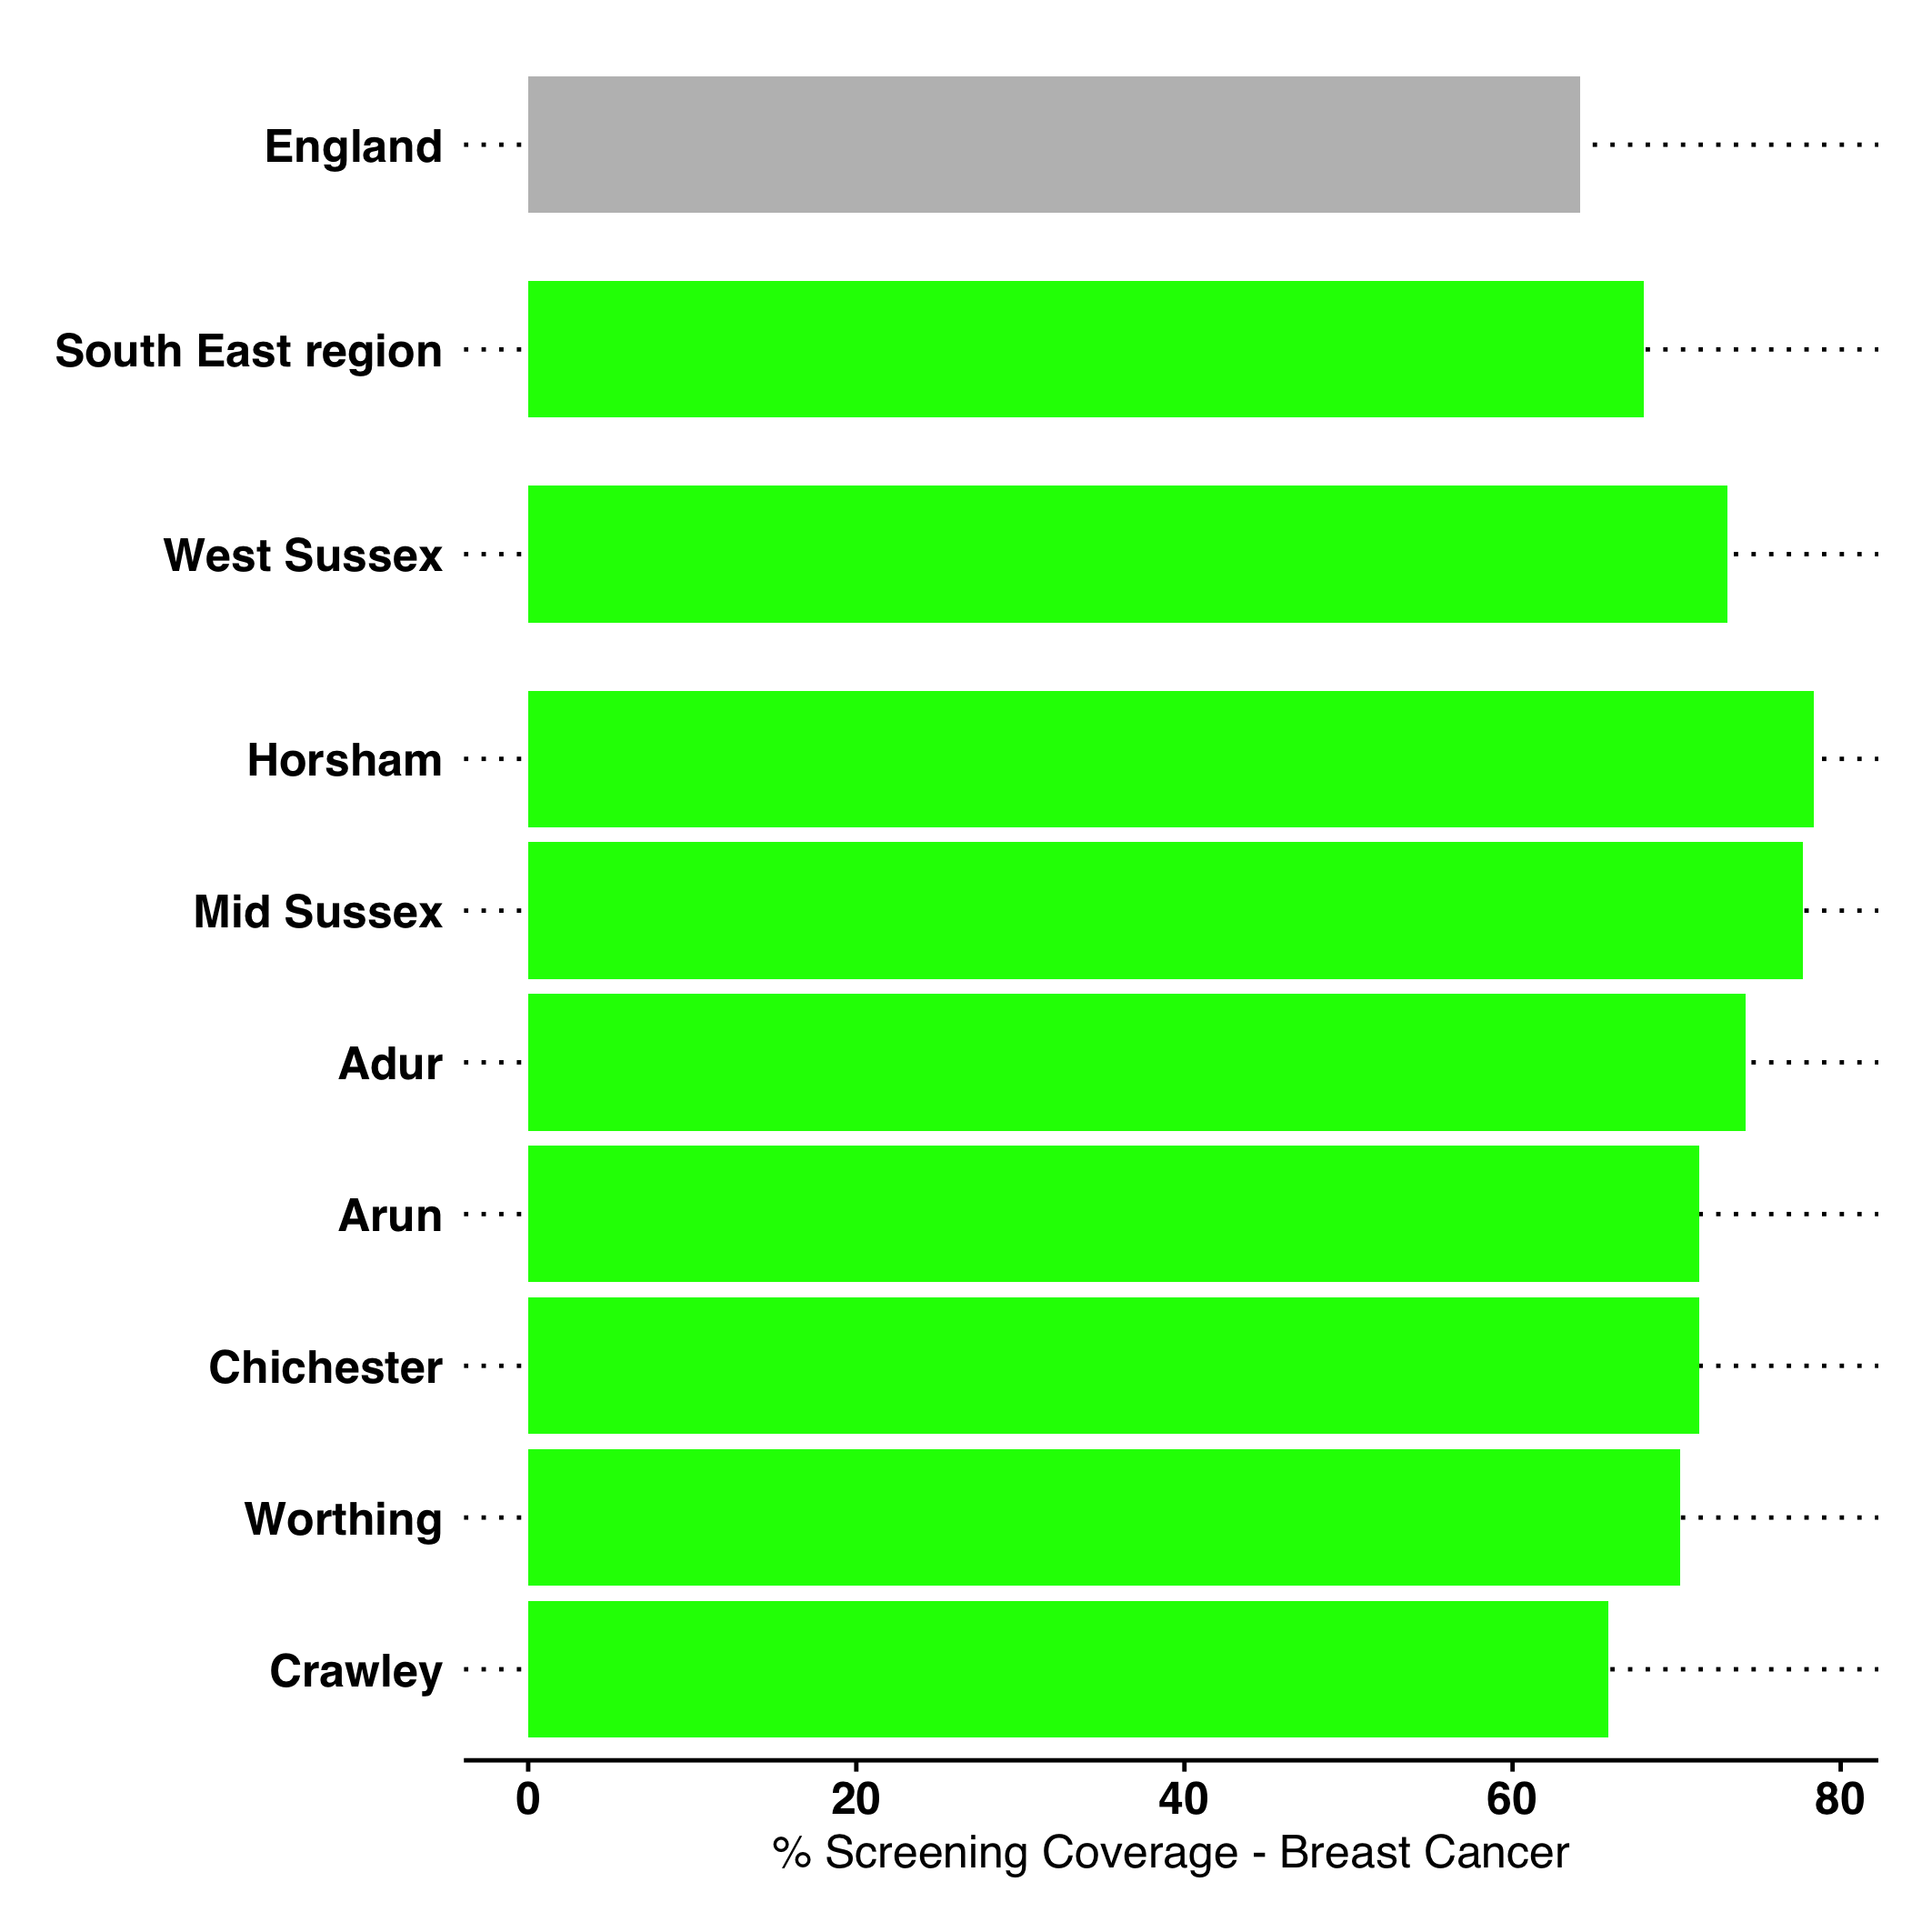
\includegraphics[width=\textwidth]{images/breast_cancer_rag_bar.png}
        \caption{Breast cancer screening coverage 2020/21 West Sussex Local Authorities}
        \label{fig:breast:rag}
    \end{subfigure}
    \begin{subfigure}[b]{0.32\textwidth}
        \centering
        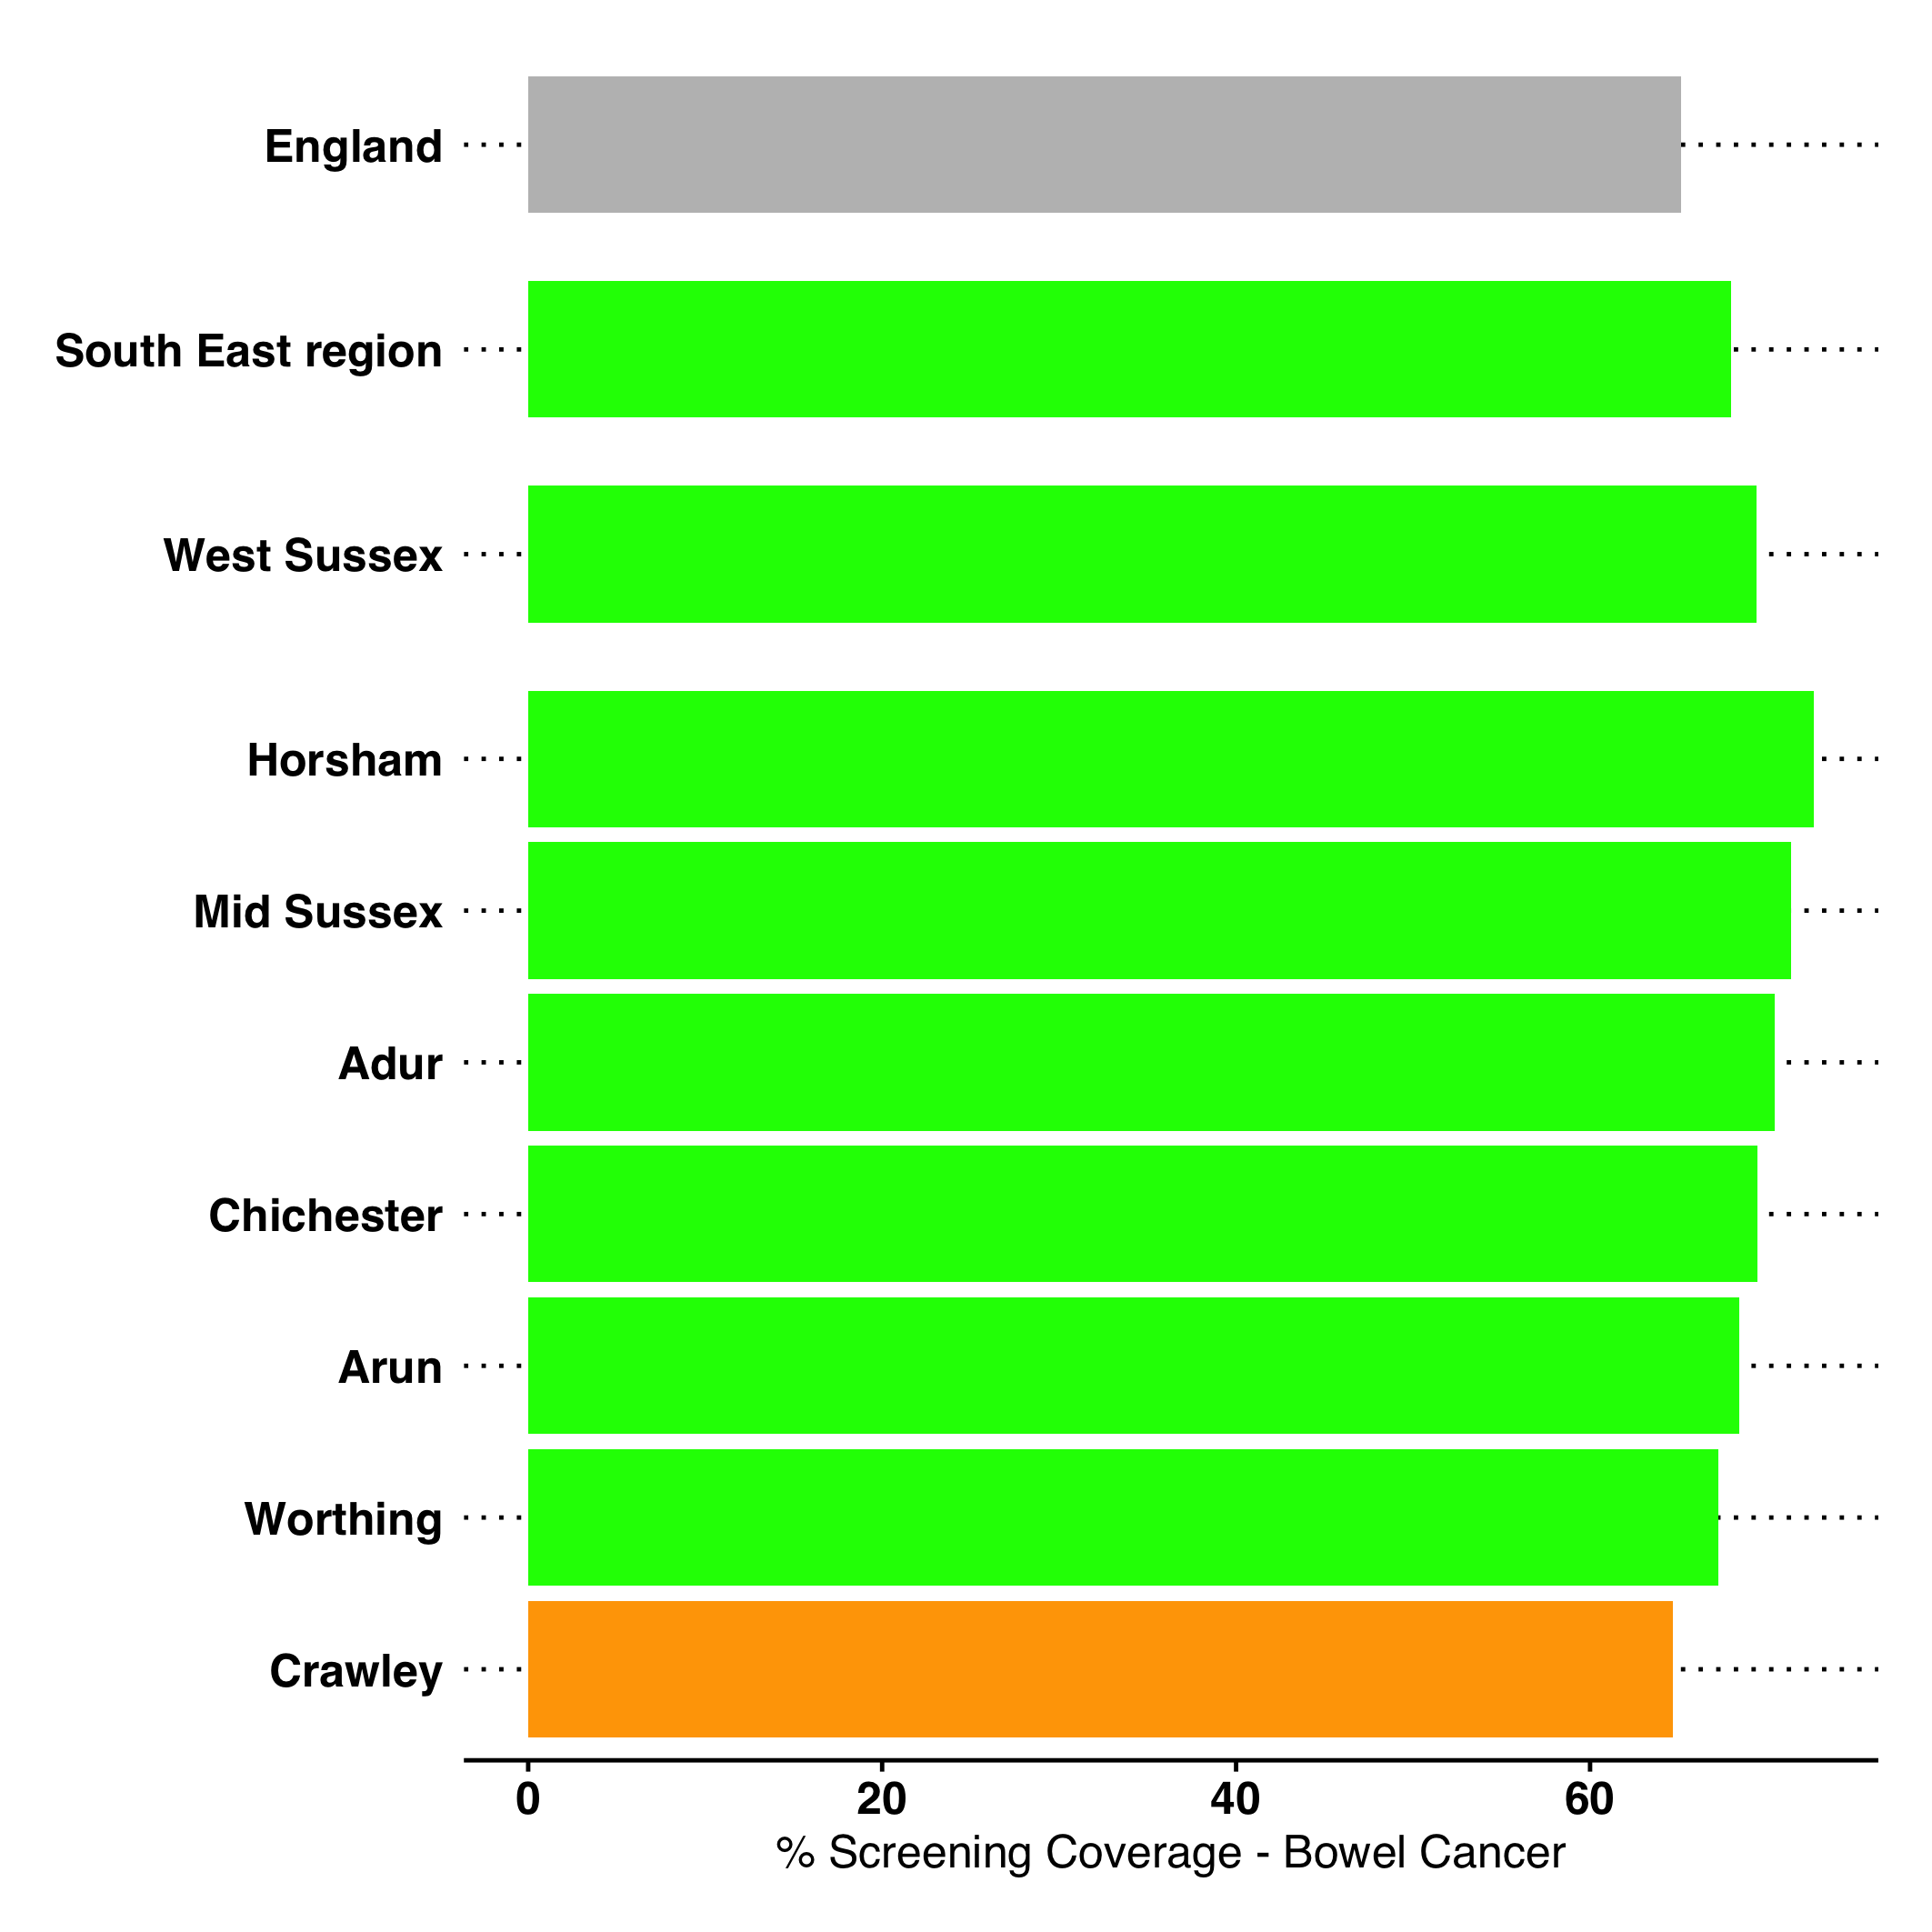
\includegraphics[width=\textwidth]{images/bowel_cancer_rag_bar.png}
        \caption{Bowel cancer screening coverage 2020/21 West Sussex Local Authorities}
        \label{fig:bowel:rag}
    \end{subfigure}
    \begin{subfigure}[b]{0.32\textwidth}
        \centering
        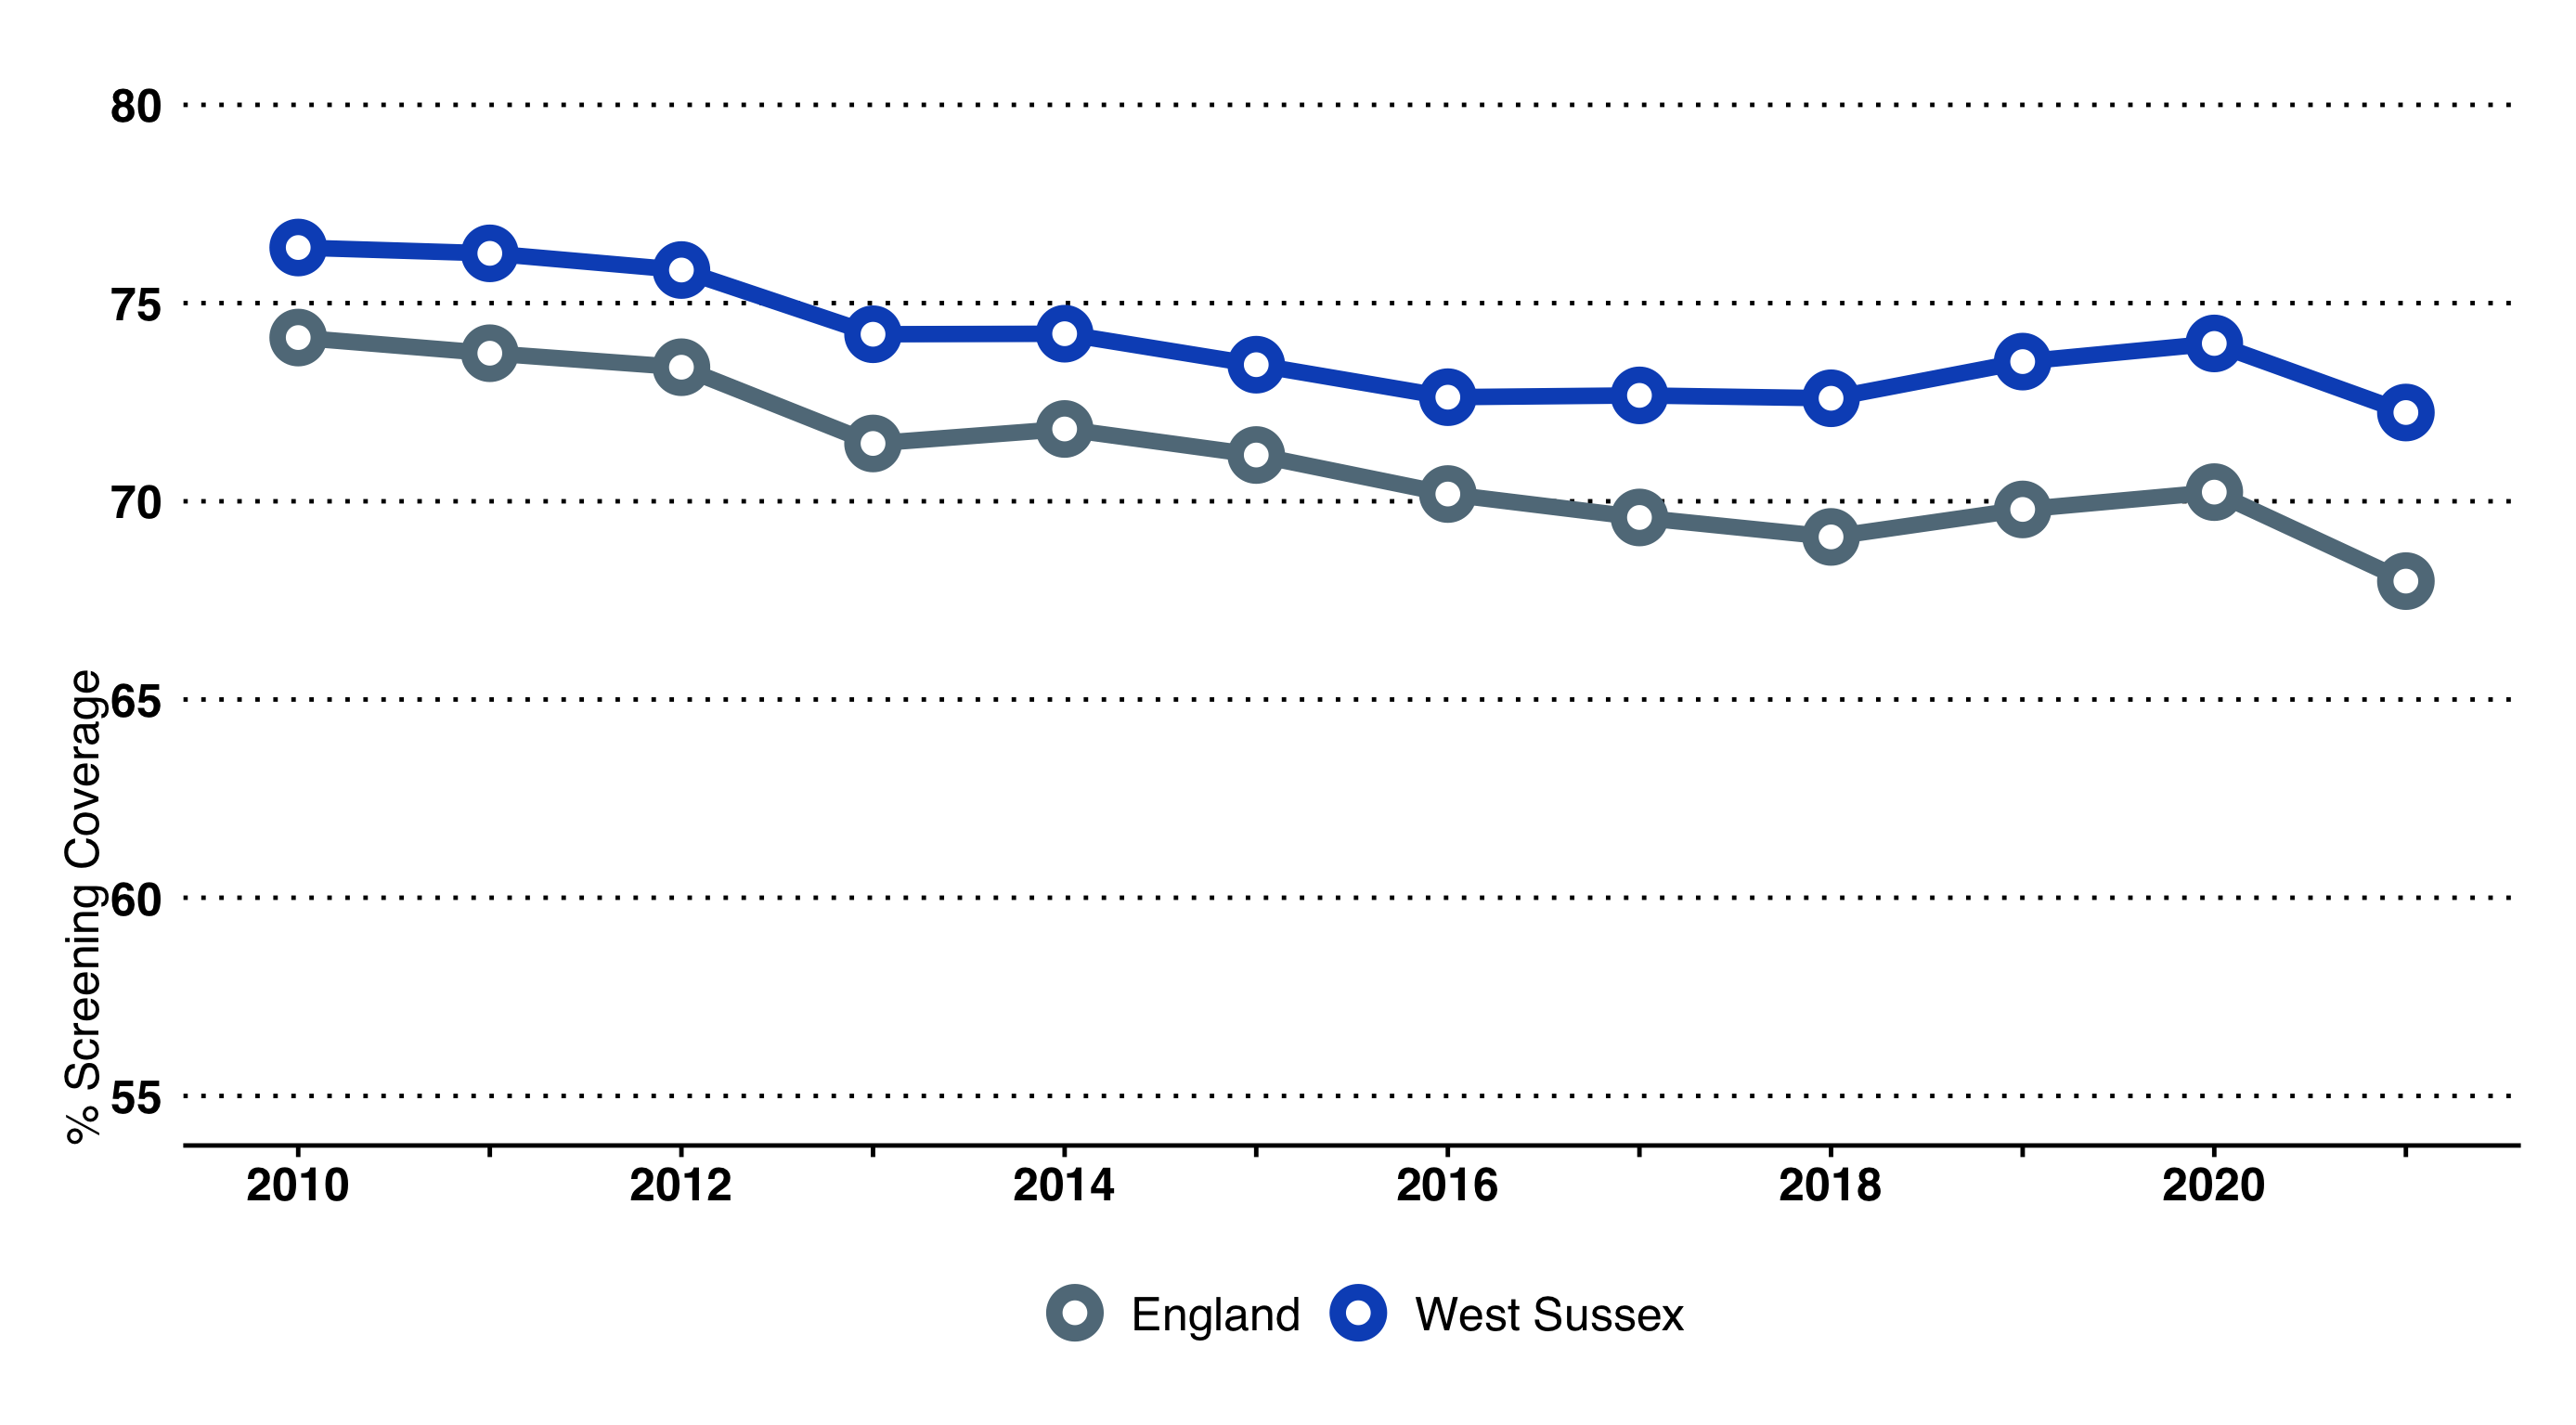
\includegraphics[width=\textwidth]{images/cervical_cancer_screening.png}
        \caption{Cervical Cancer screening coverage - West Sussex and England over time}
        \label{fig:cervical:time}
    \end{subfigure}
    \begin{subfigure}[b]{0.32\textwidth}
        \centering
        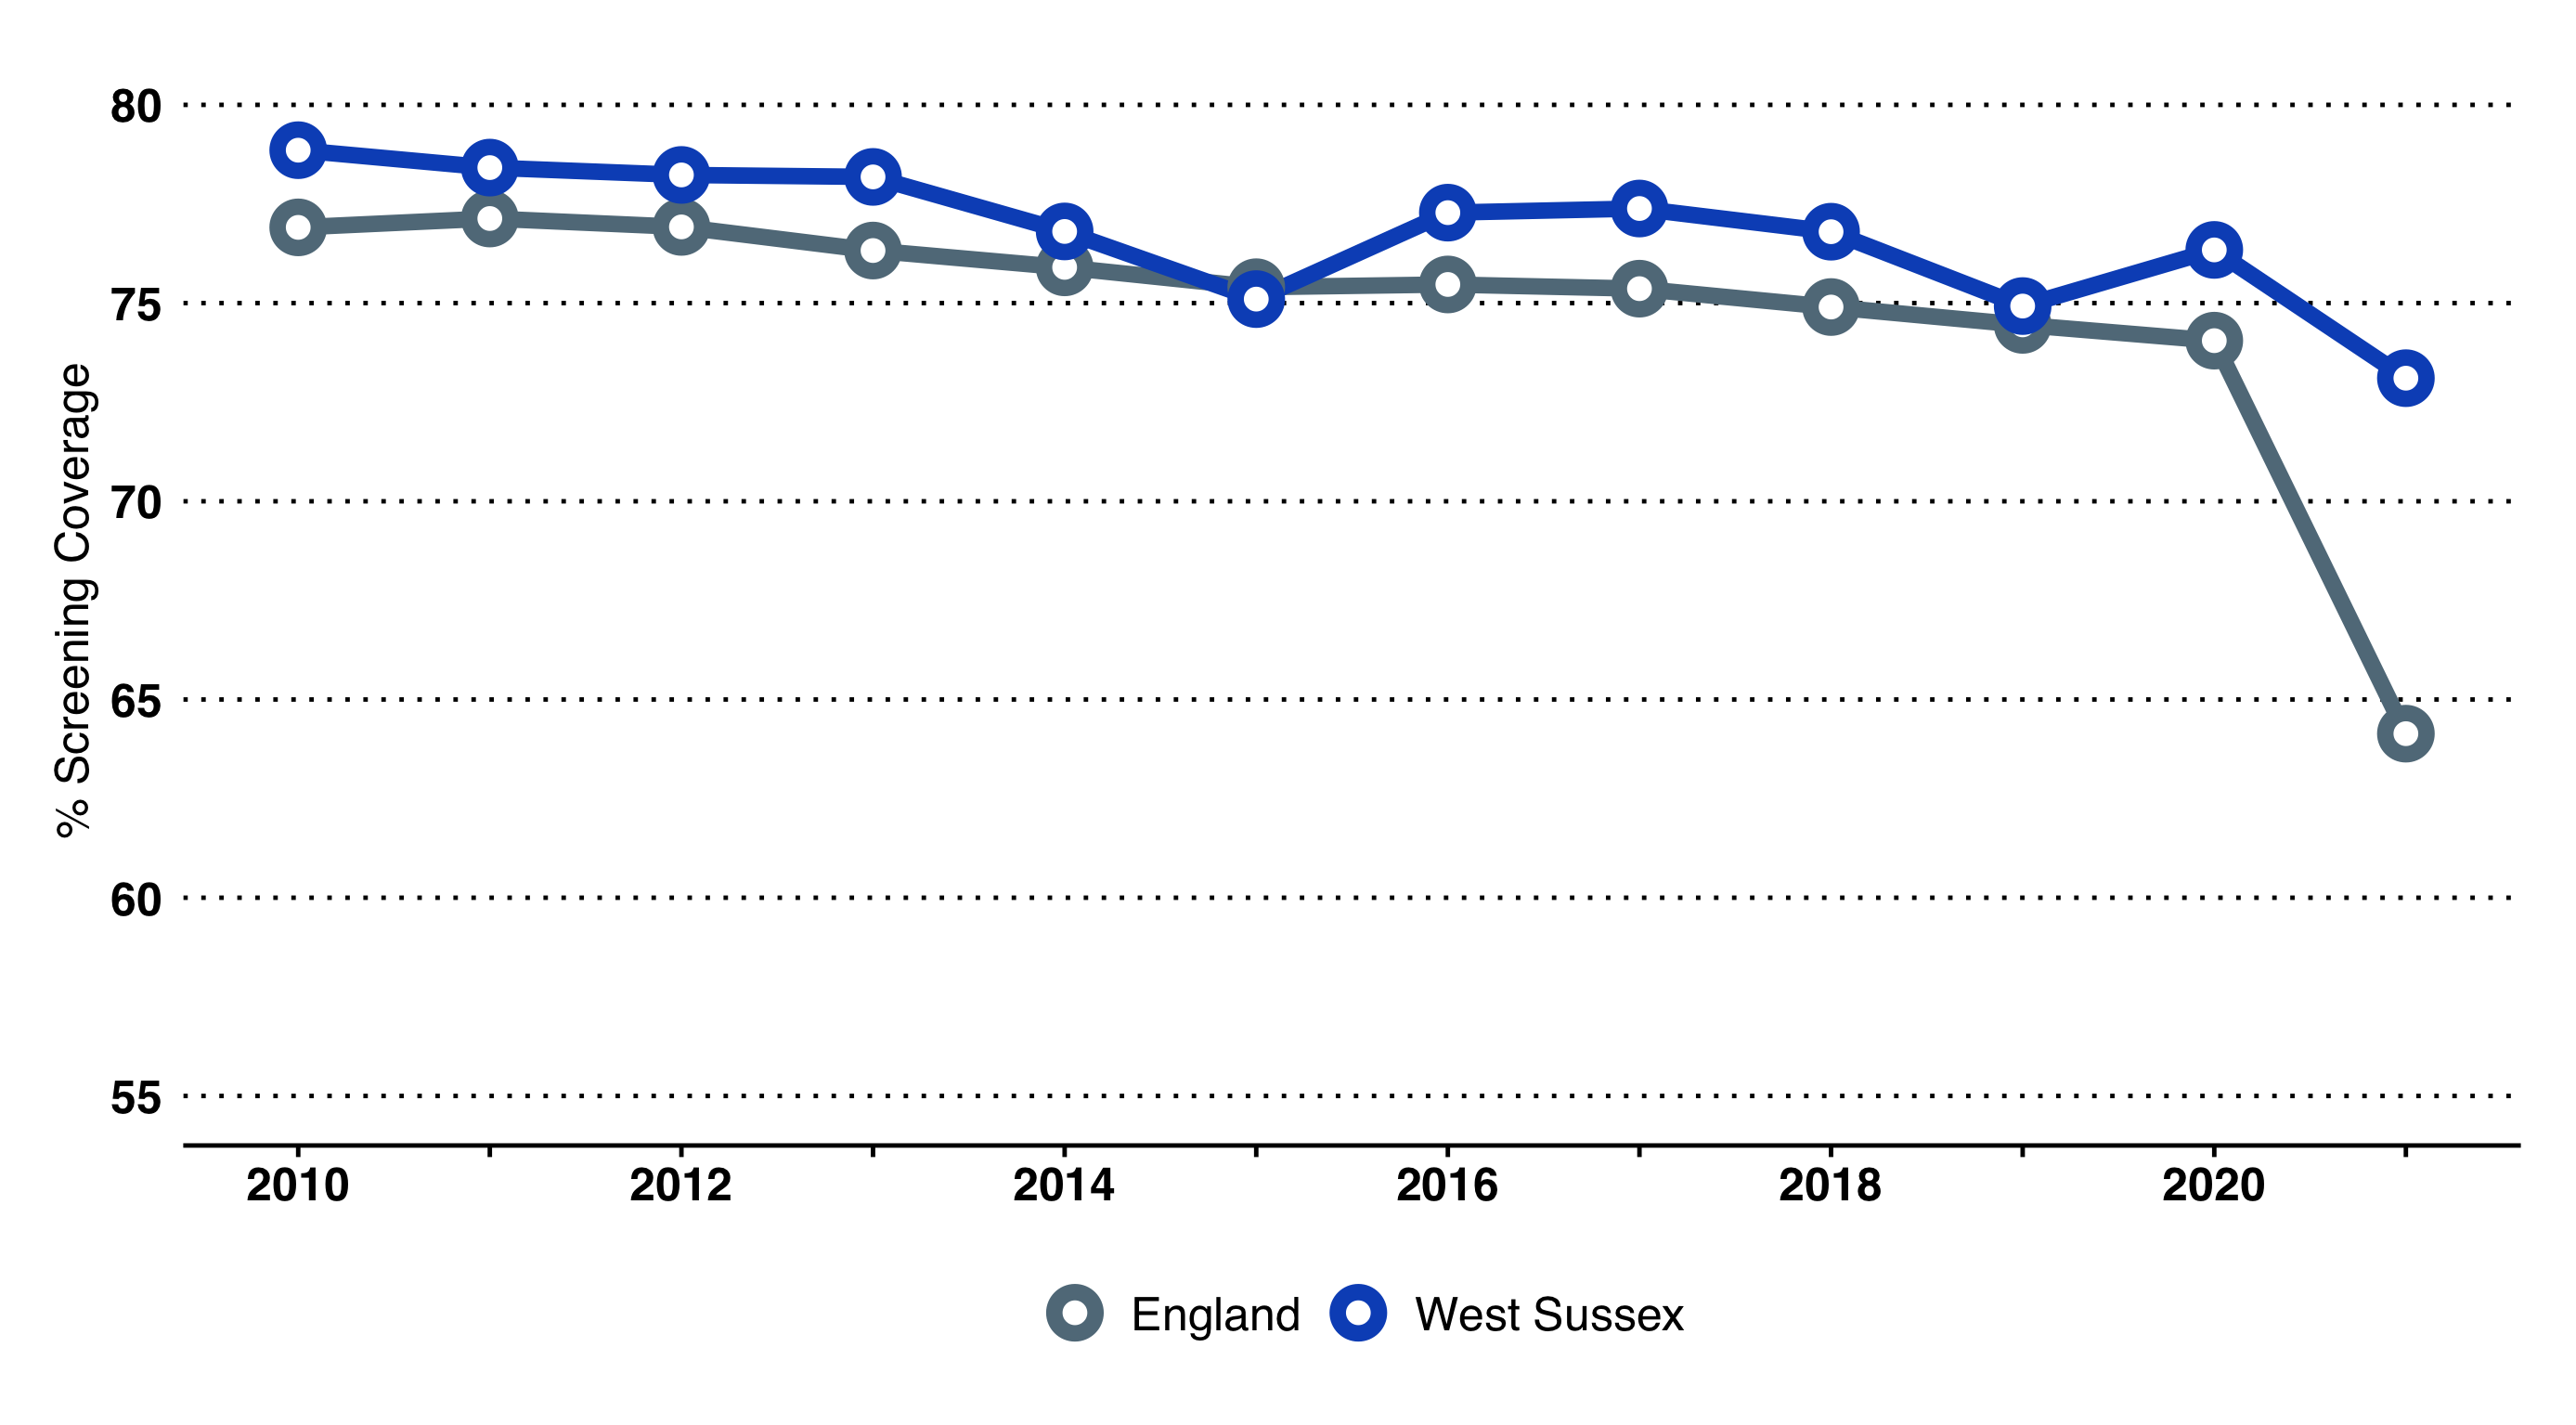
\includegraphics[width=\textwidth]{images/breast_cancer_screening.png}
        \caption{Breast Cancer screening coverage - West Sussex and England over time}
        \label{fig:breast:time}
    \end{subfigure}
    \begin{subfigure}[b]{0.32\textwidth}
        \centering
        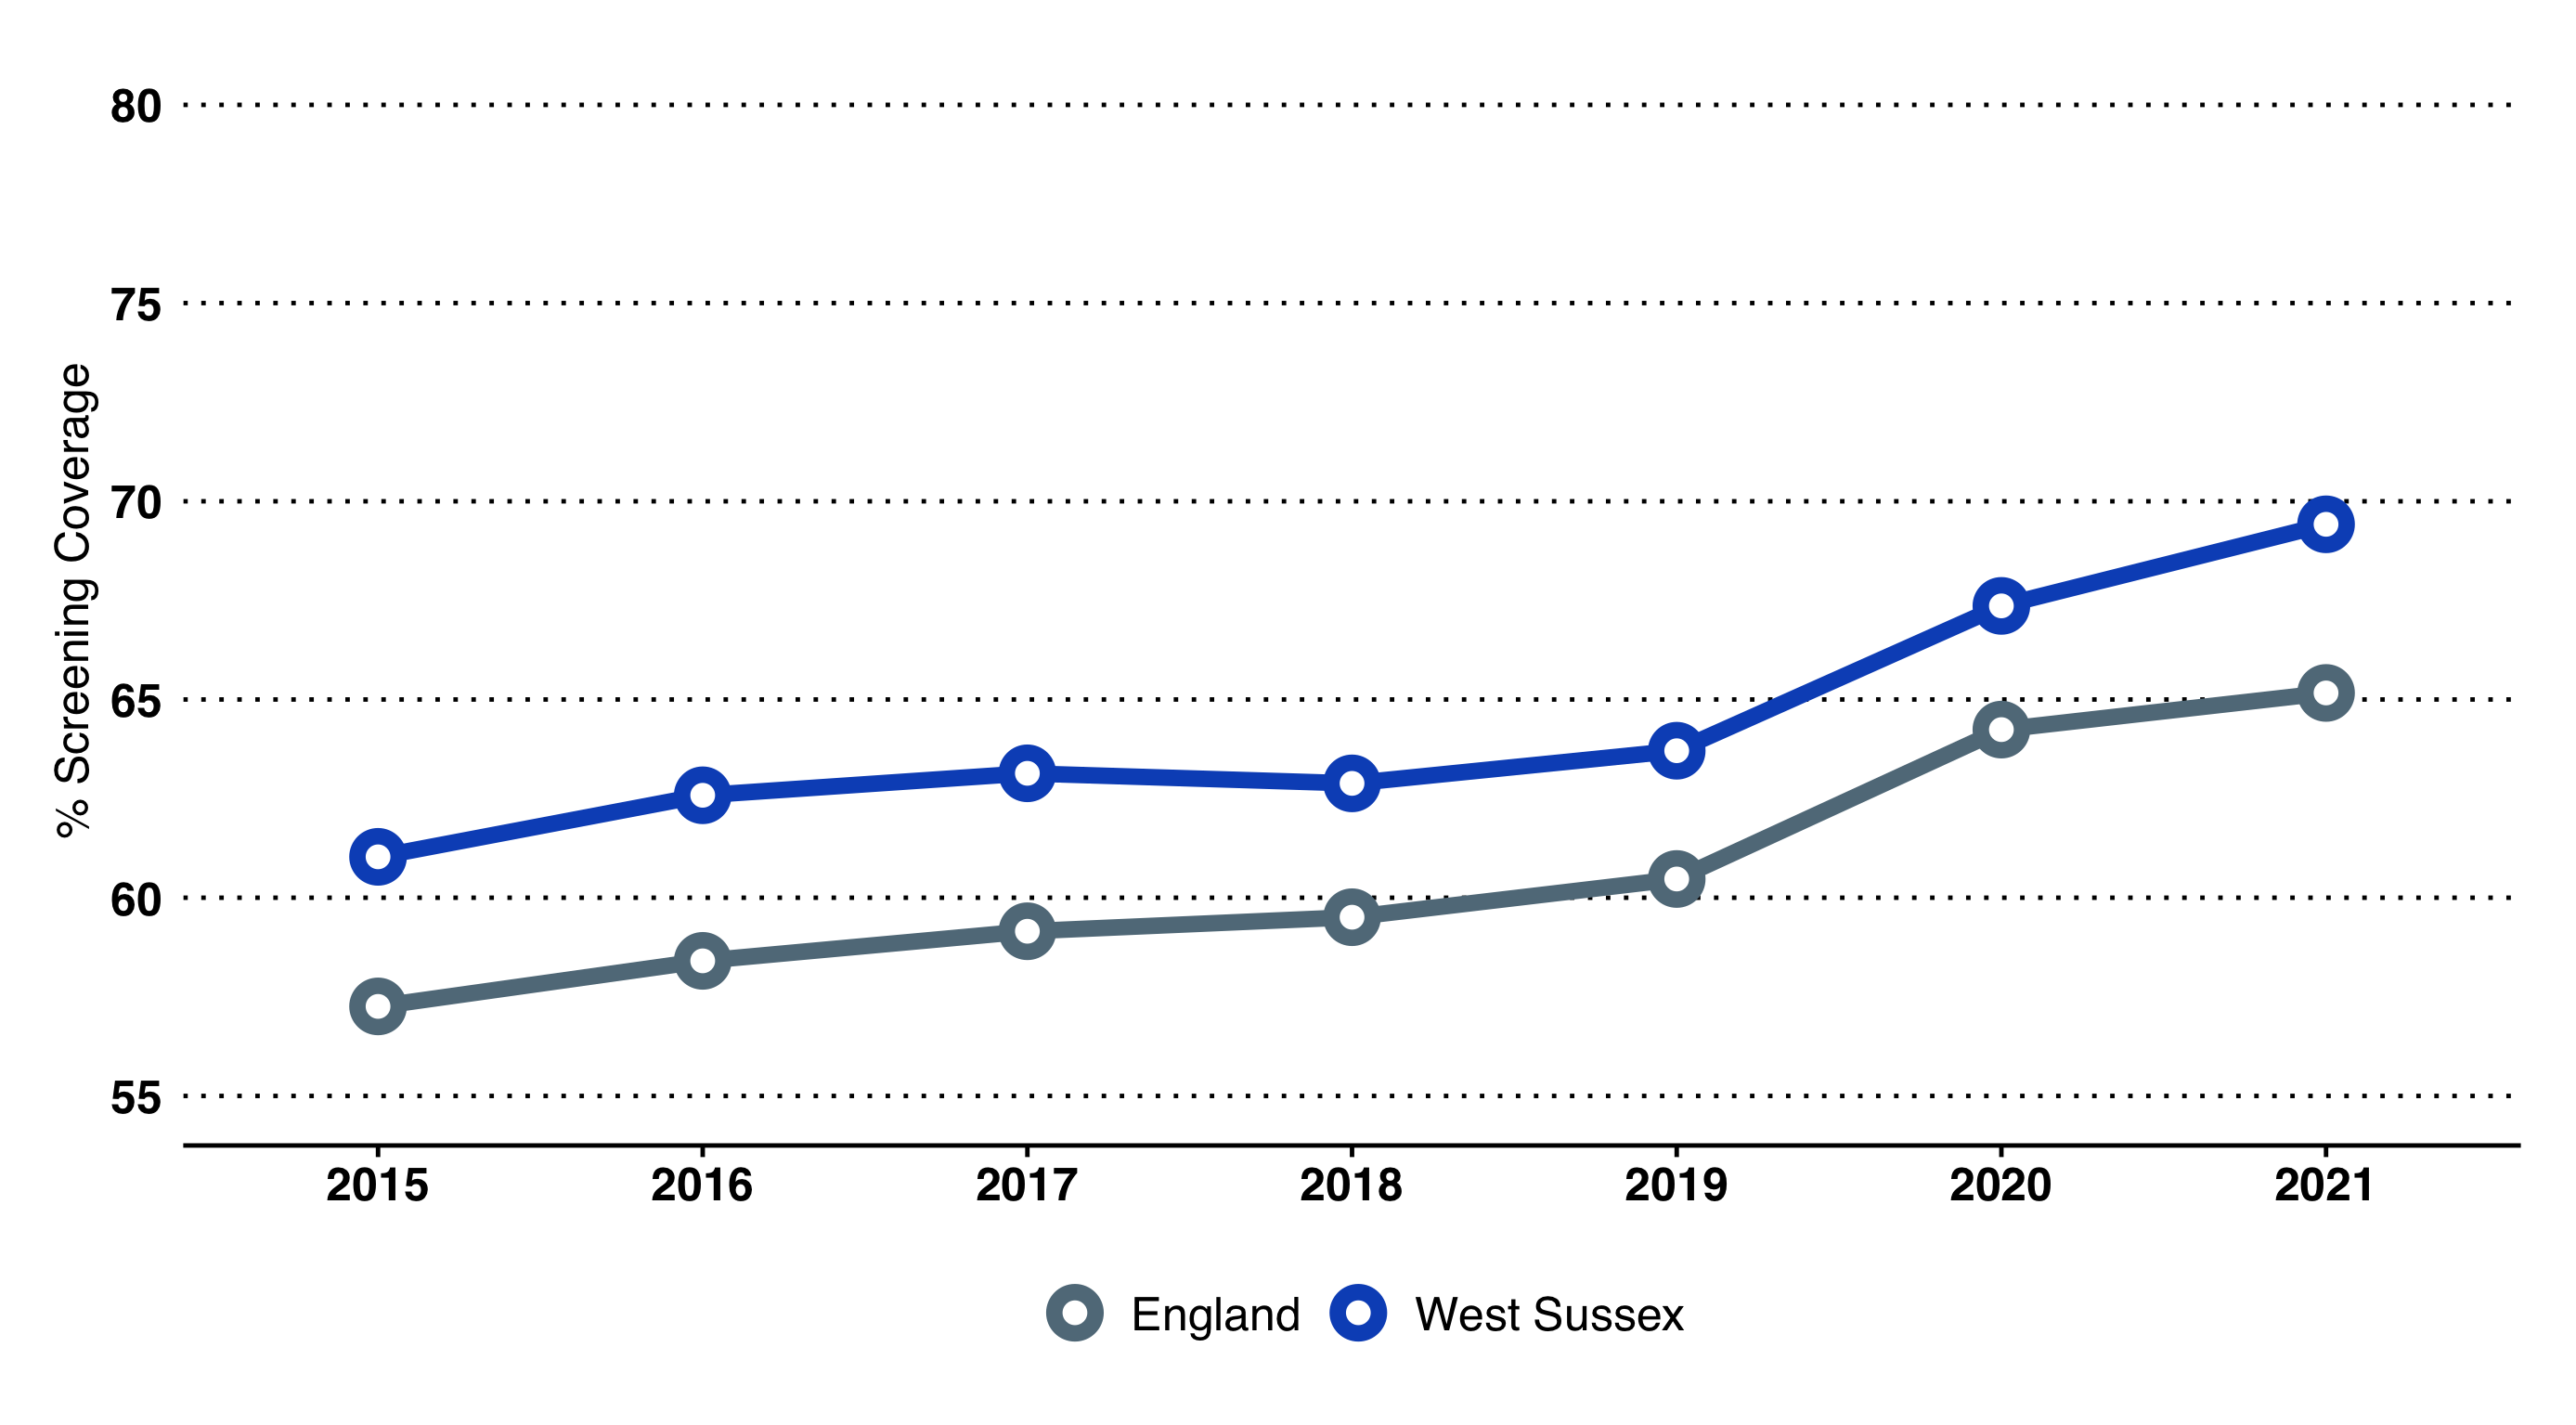
\includegraphics[width=\textwidth]{images/bowel_cancer_screening.png}
        \caption{Bowel Cancer screening coverage - West Sussex and England over time}
        \label{fig:bowel:time}
    \end{subfigure}
\end{figure*}

% Cervical - 

% \begin{figure}
%     \caption{Breast cancer screening coverage 2019/20 West Sussex Local Authorities}
%     \centering
%     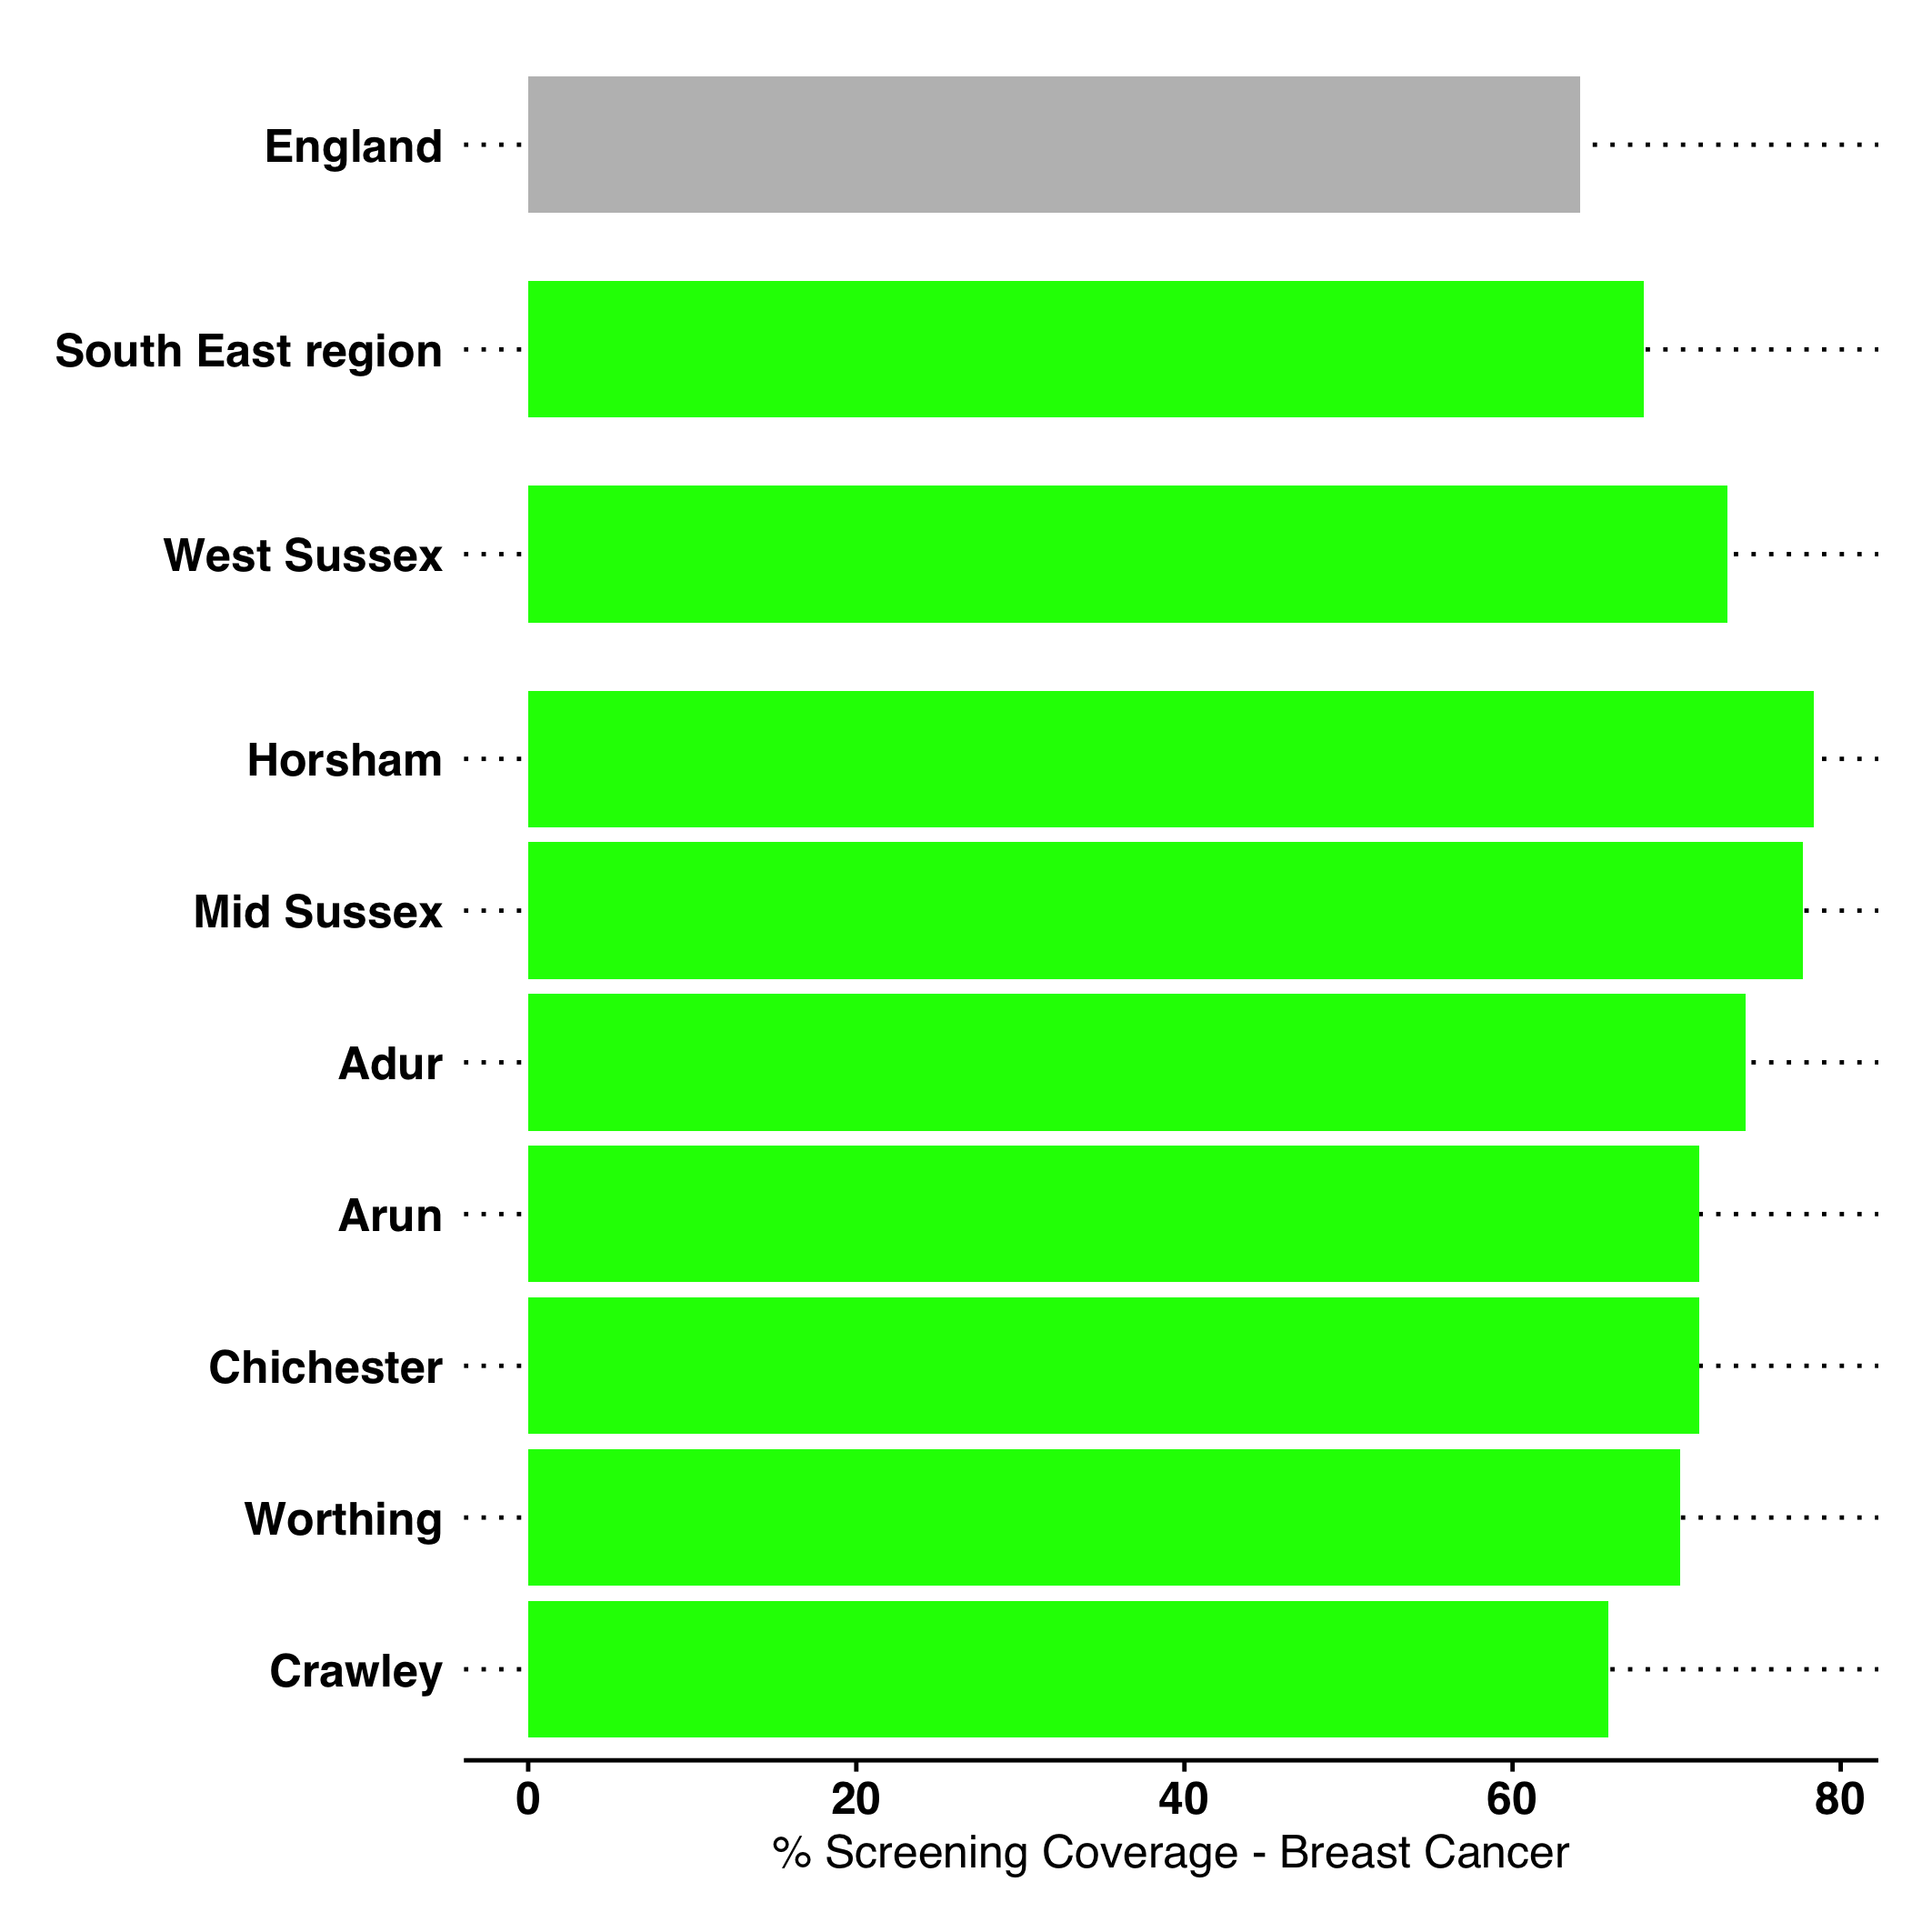
\includegraphics[width=\linewidth]{images/breast_cancer_rag_bar.png}
%     \label{fig:breast:rag}
% \end{figure}

% \begin{figure}
%     \caption{Breast Cancer screening coverage - West Sussex over time}
%     \centering
%     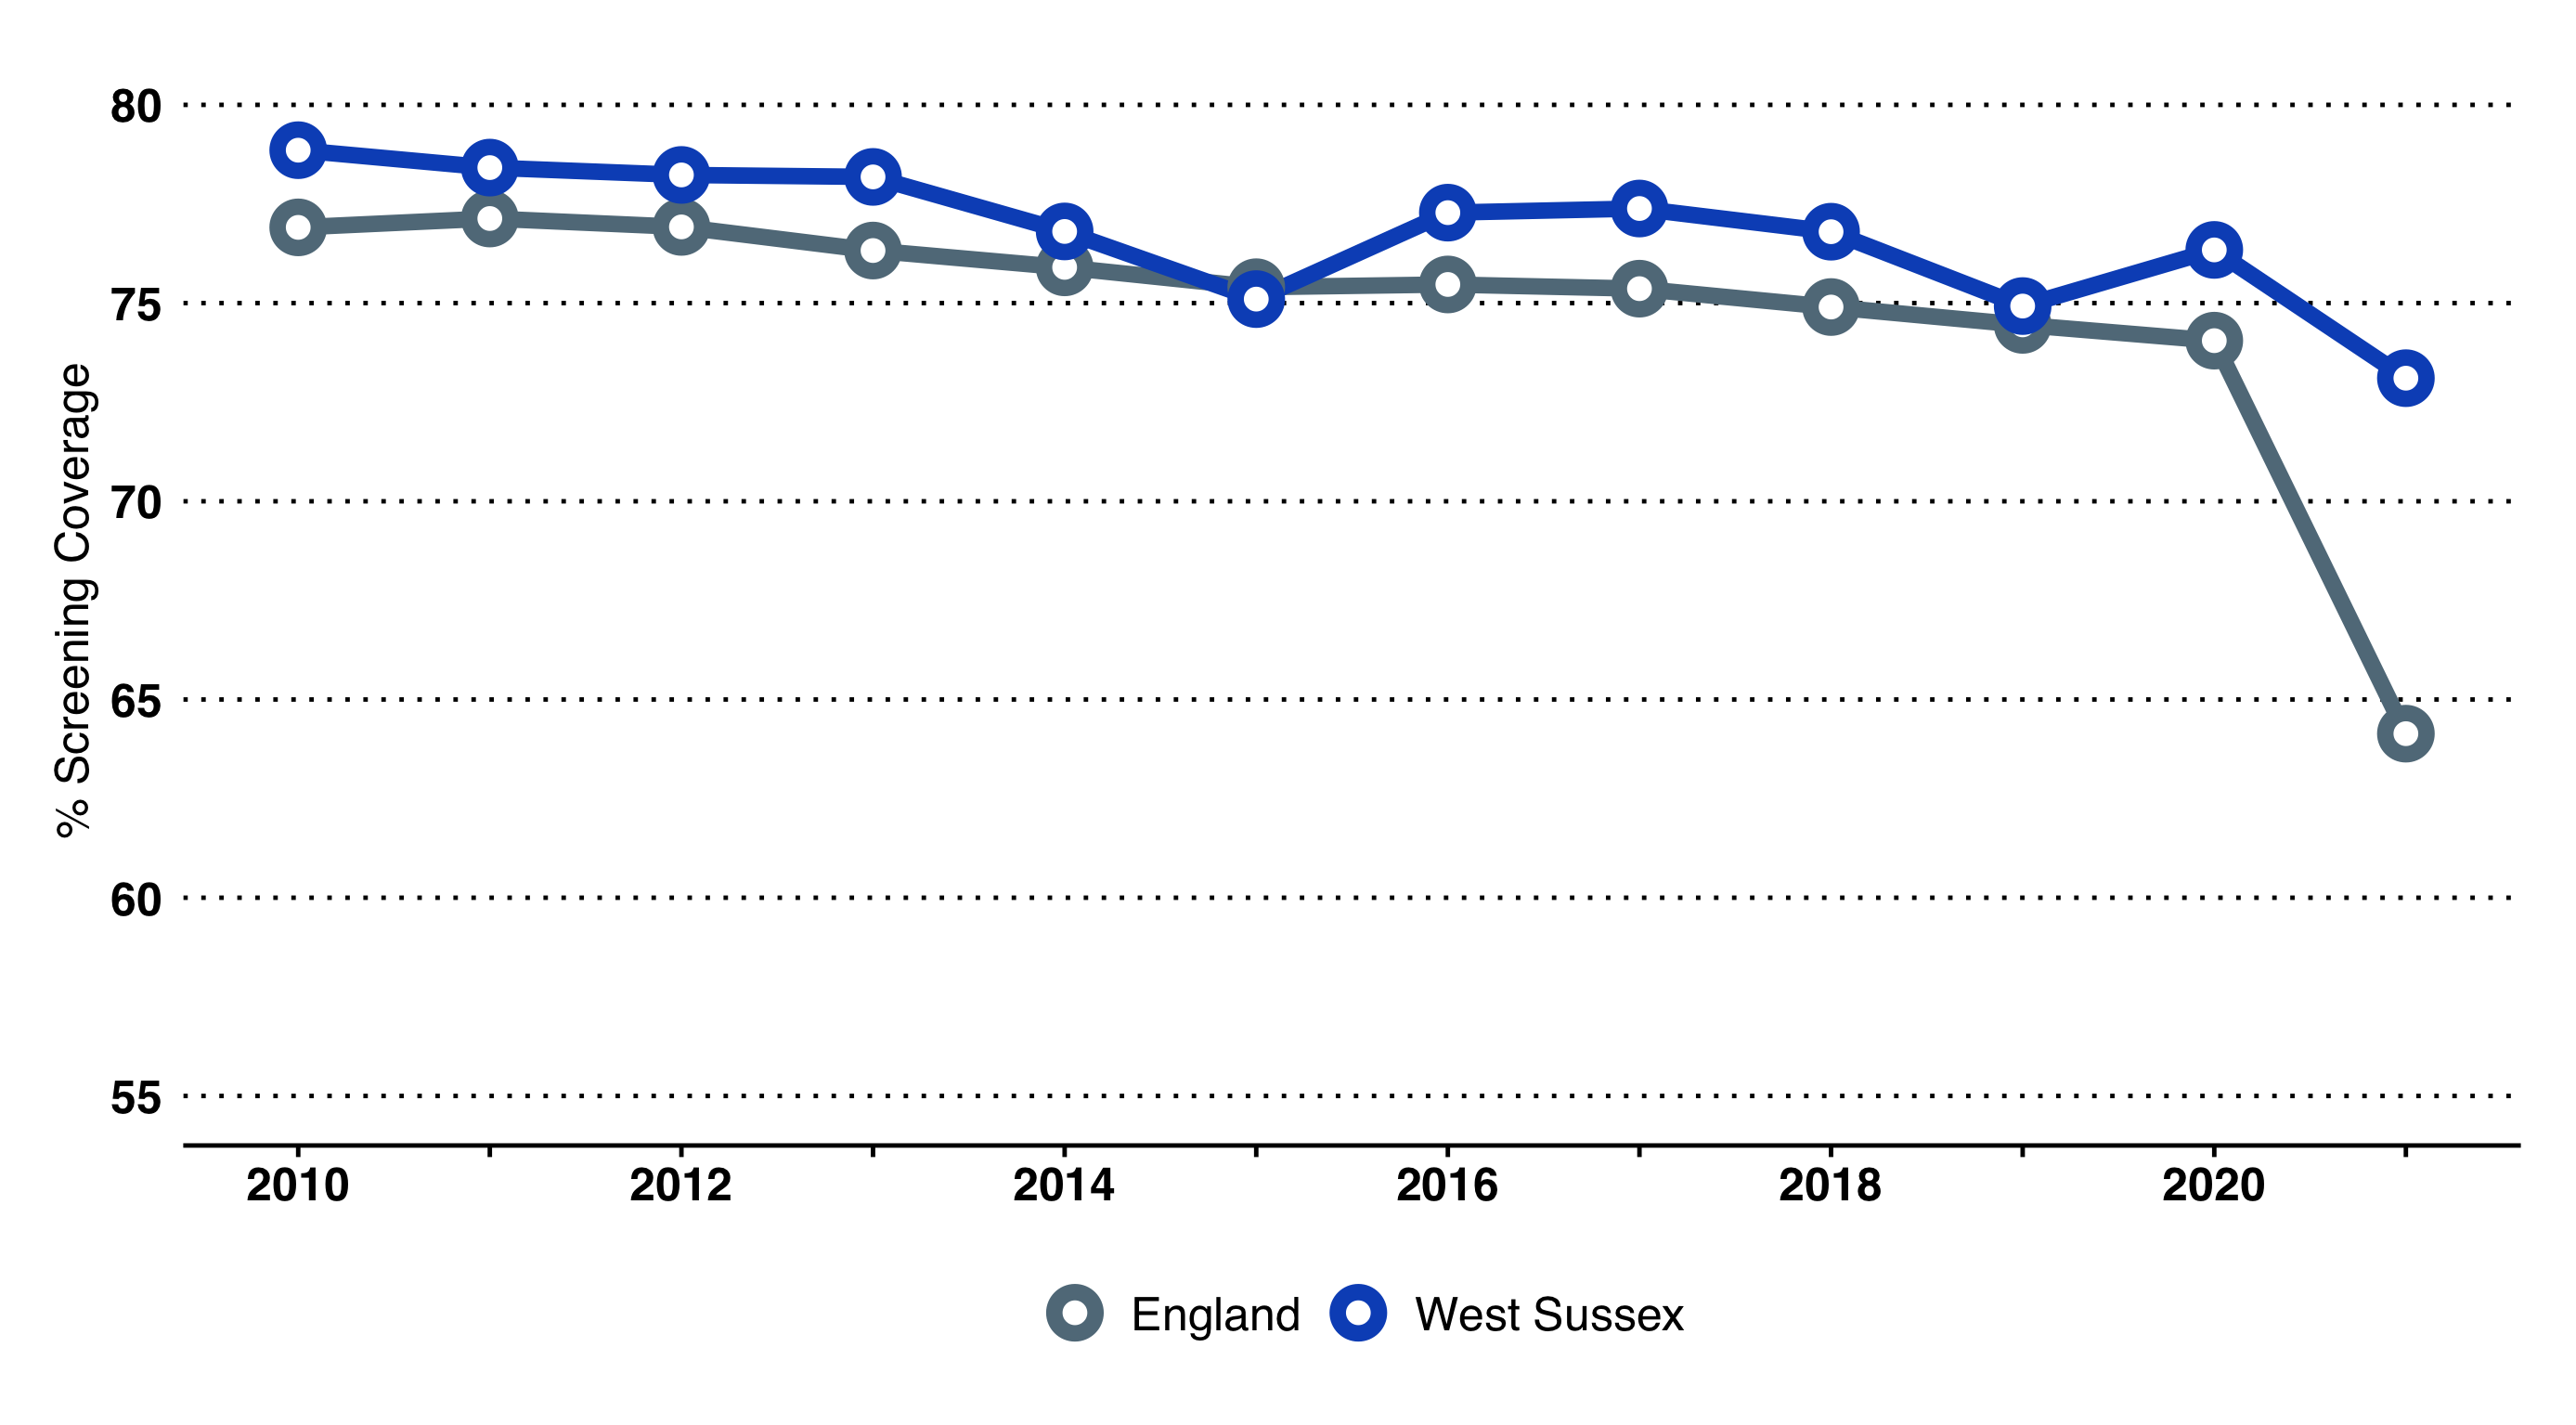
\includegraphics[width=\linewidth]{images/breast_cancer_screening.png}
%     \label{fig:breast:time}
% \end{figure}

% Breast - The screening rate at county-level for breast cancer is 74.9\% (Crawley, 70.3\%)(PHOF reference C24a). Recent issues with the West Sussex breast programme's round length may explain the decline in screening coverage.

% \begin{figure}
%     \caption{Bowel cancer screening coverage 2019/20 West Sussex Local Authorities}
%     \centering
%     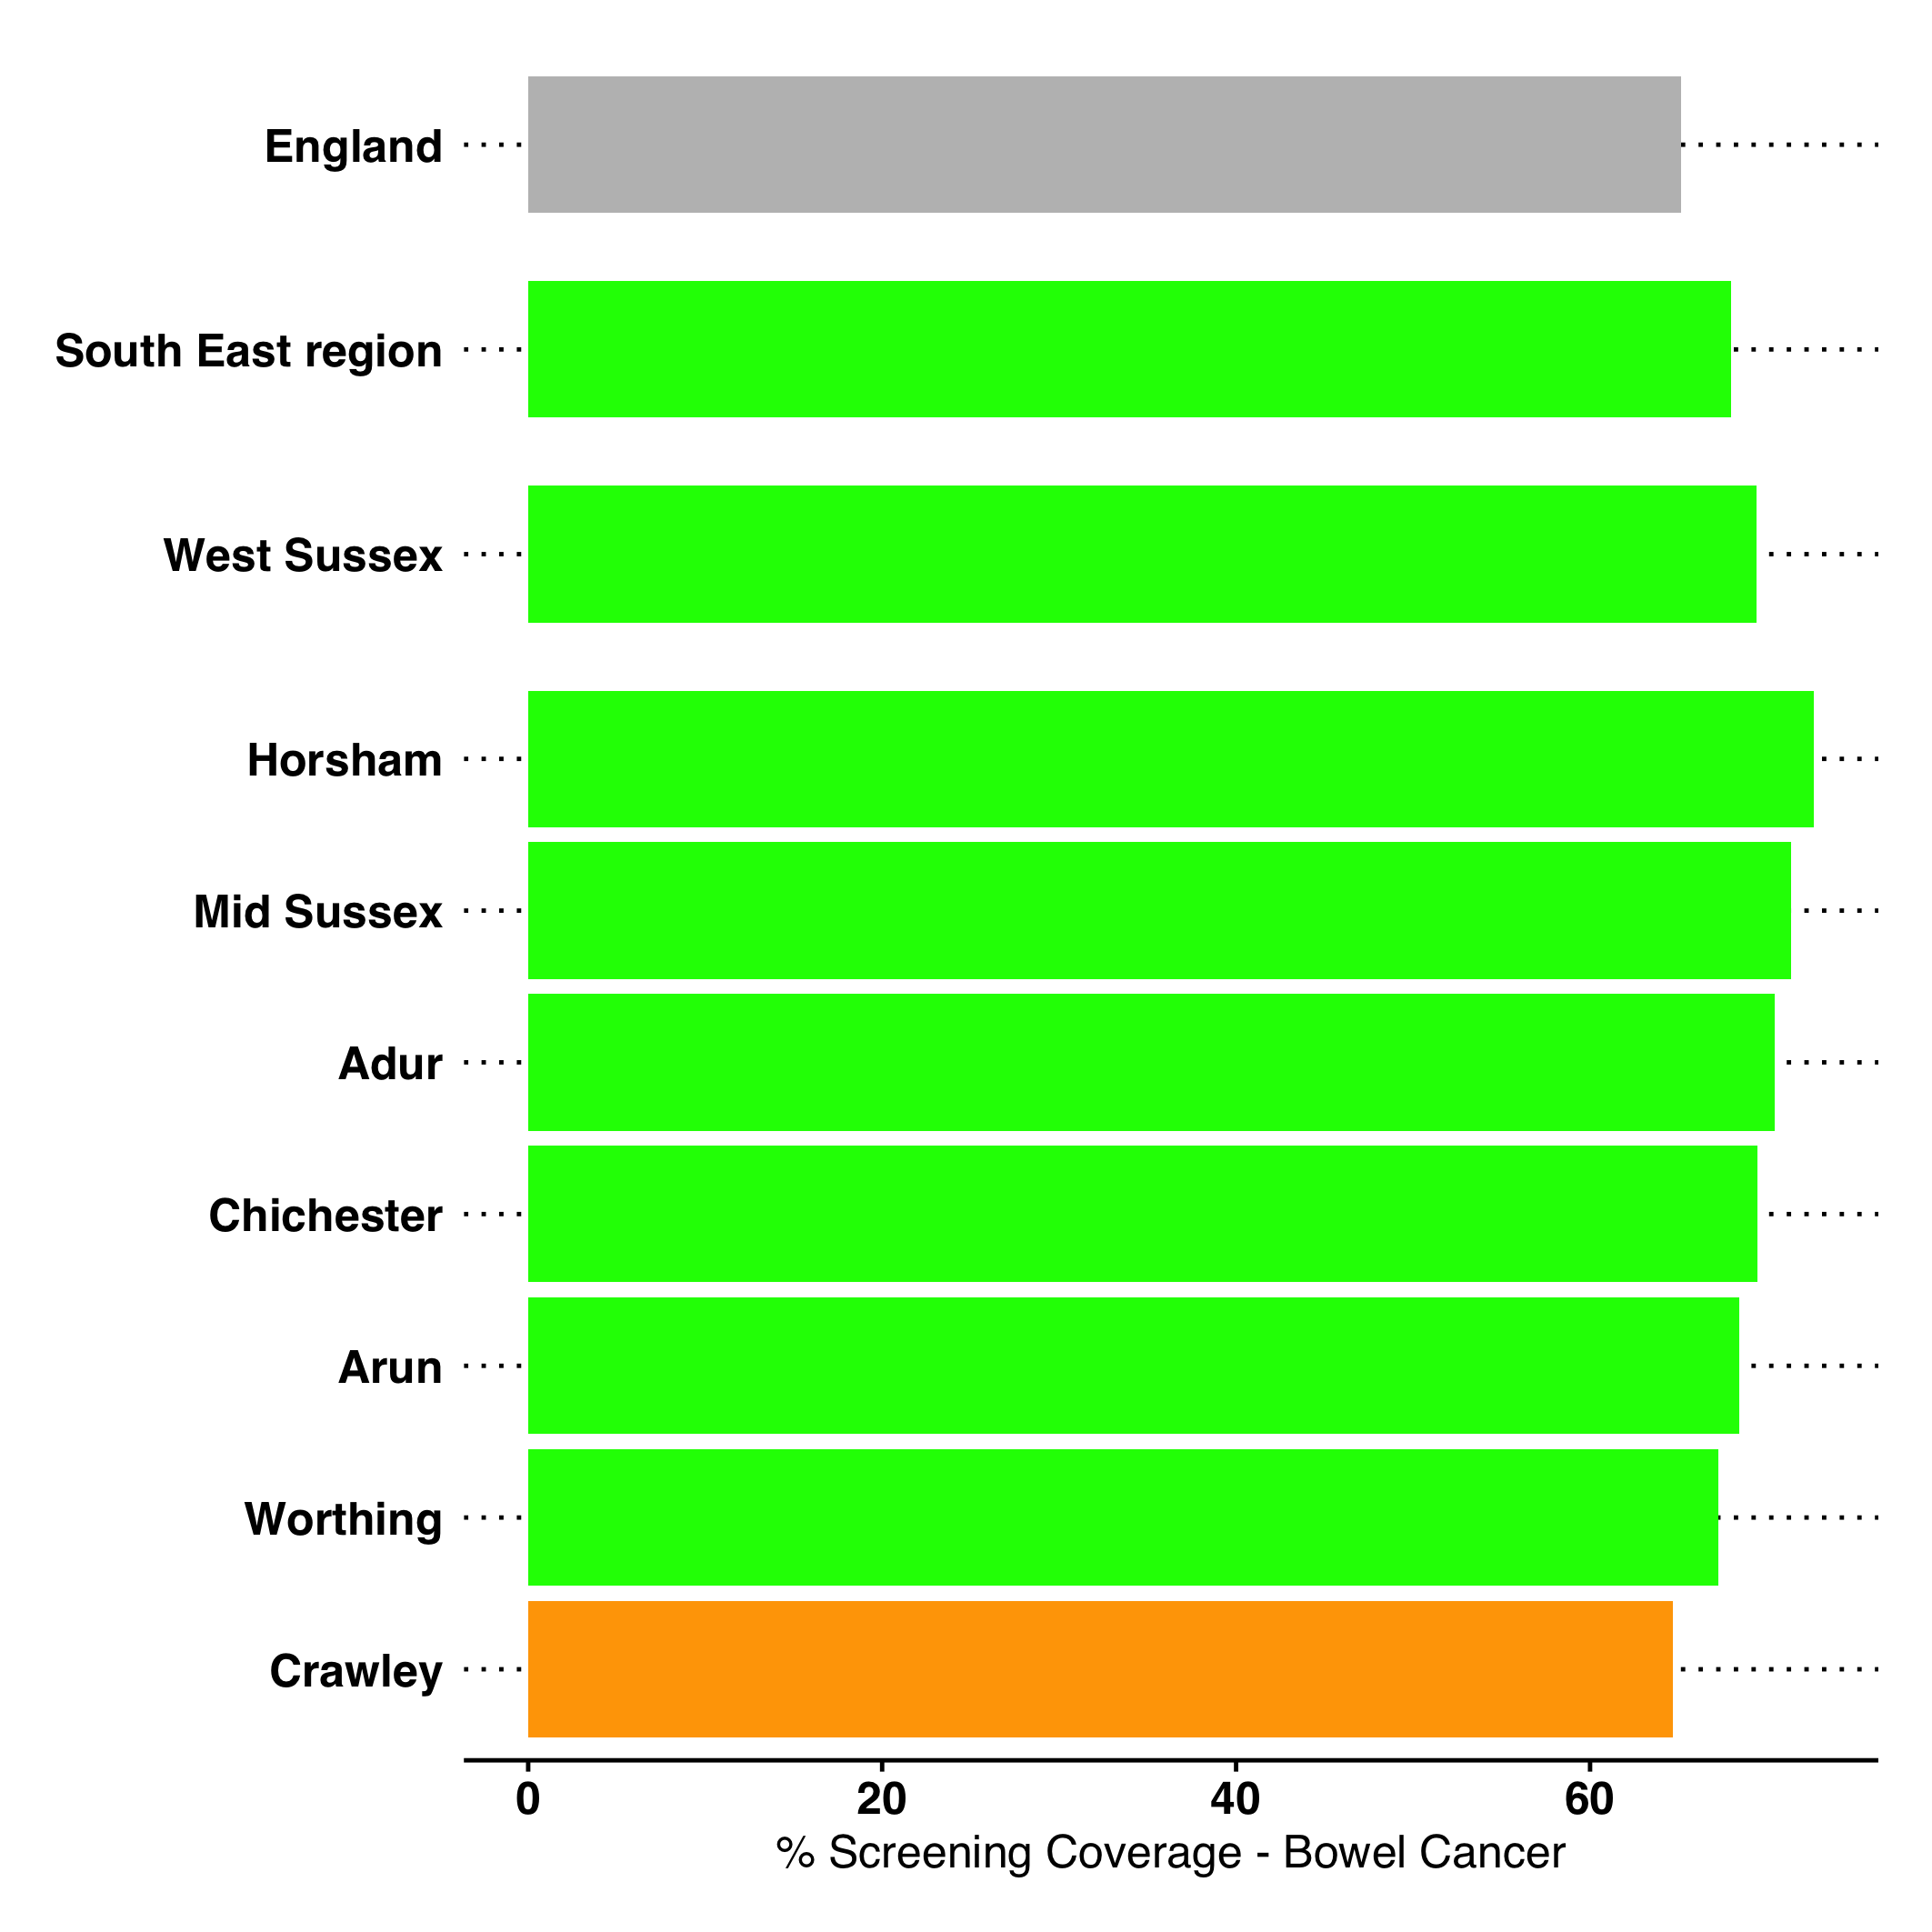
\includegraphics[width=\linewidth]{images/bowel_cancer_rag_bar.png}
%     \label{fig:bowel:rag}
% \end{figure}

% \begin{figure}
%     \caption{Bowel cancer screening coverage - West Sussex over time}
%     \centering
%     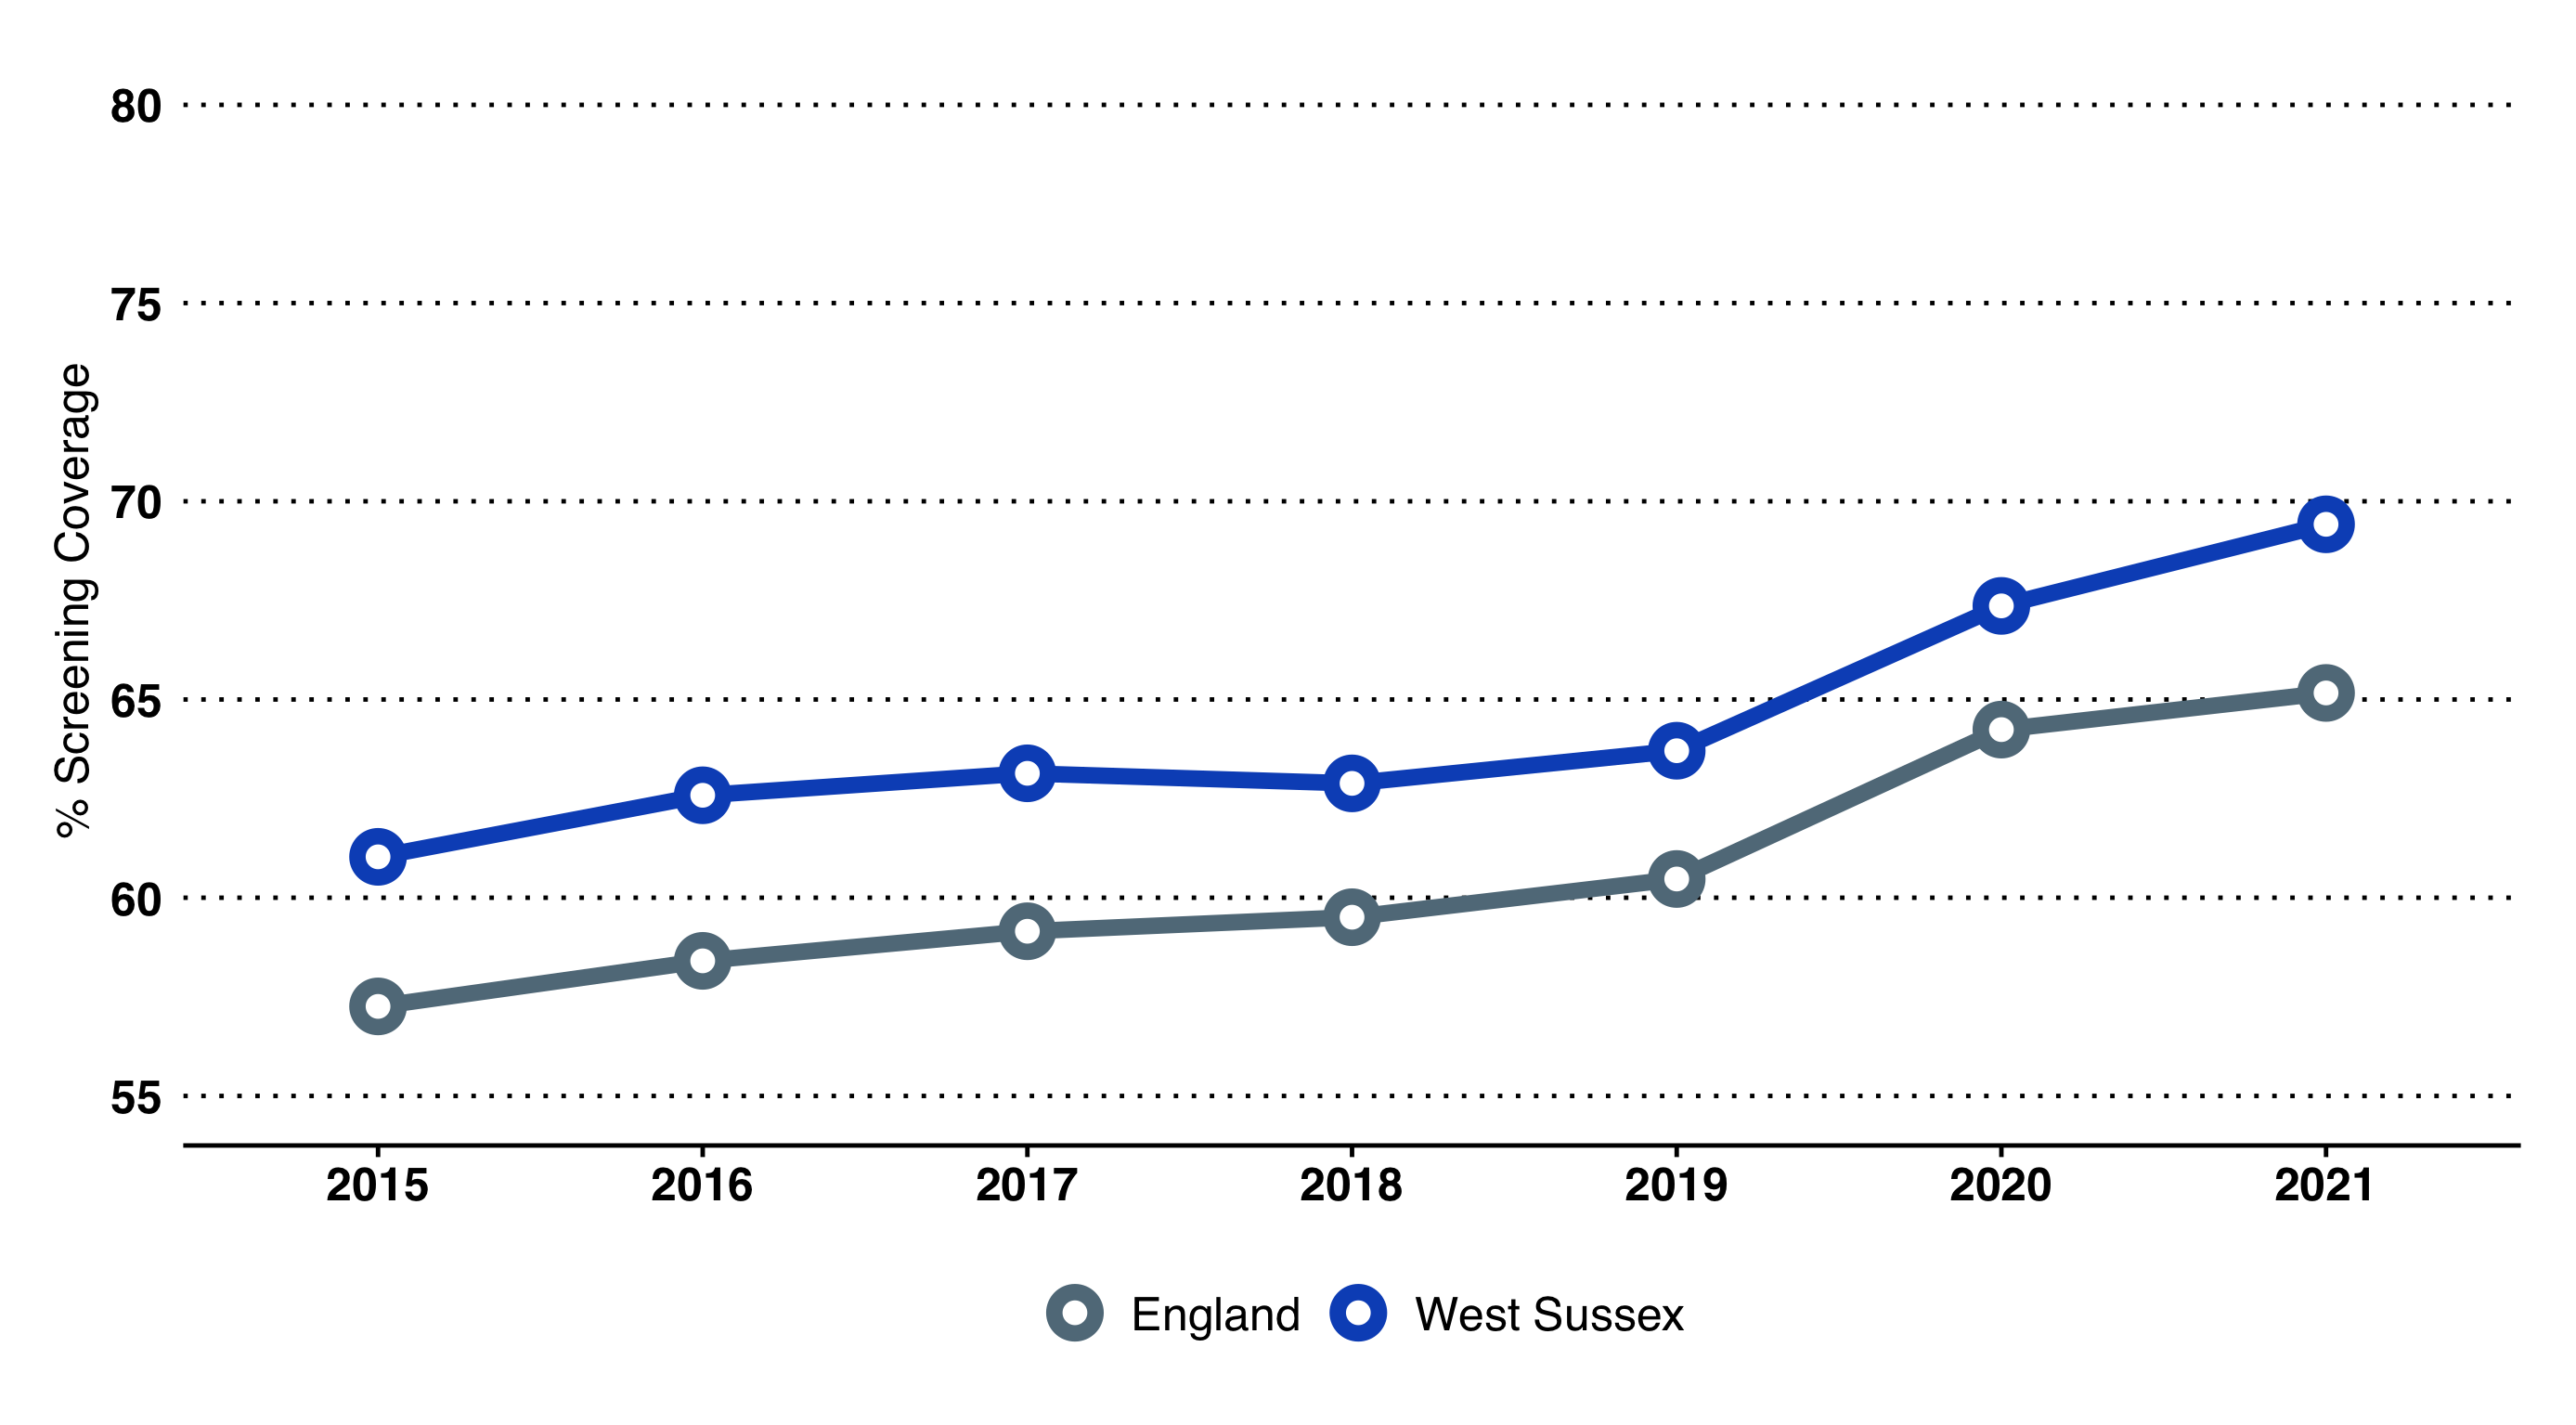
\includegraphics[width=\linewidth]{images/bowel_cancer_screening.png}
%     \label{fig:bowel:time}
% \end{figure}

% Bowel - 

\clearpage

\subsection{Mental Health}
Many of the prevalence assumptions for adult mental health conditions are derived from national surveys and research. Of particular note is the Adult Psychiatric Morbidity Survey (APMS). The APMS provides data on the prevalence of treated and untreated psychiatric disorders among adults (aged 16+) in households in England. The most recent survey was conducted in 2014 (McManus, Bebbington, Jenkins, \& Brugha, 2016) and is the fourth in the series (previous survey years include: 1993, 2000 and 2007).

\subsubsection{APMS Key Findings}
\begin{itemize}[noitemsep]
    \item Nationally, 1 in 6 adults (17.0\%) were identified with a common mental health disorder (CMD) in the week prior to being interviewed APMS. Applying this prevalence estimate to West Sussex, it is estimated that 121,200 adults (aged 16+) are likely to have a common mental health problem\footnote{Note that the national estimate is a synthetic estimate. Note also that a synthetic prevalence estimate of 14.4\% exists for West Susssex, which is equivalent to approximately 102,600 people based on current population estimates.}.
    \item Women were more likely to have a common mental health disorder than men.
    \item 64.4\% of adults who were identified as having a common mental health disorder in the survey had been diagnosed by a professional.
    \item Around a third (35.6\%) of adults identified as currently with CMD by the survey have never been diagnosed. This may reflect unmet need, or demonstrate how perceptions of mental health vary.
\end{itemize}

\begin{table*}
    \caption{Estimates of Prevalence of Common Mental Health Disorders in West Sussex by age group (Adult Psychiatric Morbidity Survey 2014, applied to West Sussex 2020 Population estimates)}
    \centering
    \begin{tabular}{lrrrrrrrr}
        \toprule
        \ & 16-24 & 25-34 & 35-44 & 45-54 & 55-64 & 65-74 & 75+ & All \\
        \midrule
        Generalised anxiety disorder & 4,530 & 5,670 & 7,370 & 8,870 & 7,510 & 4,140 & 2,470 & 42,050 \\
        Depressive episode & 1,660 & 3,250 & 4,380 & 5,470 & 5,040 & 2,170 & 1,280 & 23,520 \\
        Phobias & 2,380 & 3,070 & 3,210 & 3,280 & 2,700 & 620 & 490 & 17,100 \\
        Obsessive compulsive disorder & 1,300 & 1,300 & 1,710 & 1,940 & 1,760 & 310 & 300 & 9,260 \\
        Panic disorder & 860 & 460 & 320 & 610 & 590 & 720 & 590 & 4,280 \\
        CMD-NOS (not otherwise specified) & 6,050 & 8,460 & 8,760 & 10,570 & 9,500 & 5,380 & 4,830 & 55,590 \\
        Any CMD & 13,600 & 17,660 & 20,620 & 23,200 & 21,110 & 11,900 & 8,680 & 121,160 \\
        \bottomrule
    \end{tabular}
    \label{tab:wa:cmd}
\end{table*}


 
\subsubsection{Severe Mental Illness} The mental health register is a count of the total number of people with schizophrenia, bipolar disorder and other psychoses. In 2020/21, the recorded disease prevalence for mental health was 0.91\% in West Sussex CCG, which is lower than that of England as a whole (0.95\%).

\begin{table}
    \caption{Recorded disease prevalence for mental health conditions (schizophrenia, bipolar disorder and psychoses) (2016/17)}
    \centering
    \begin{tabular}{lrrr}
        \toprule
        \ & List Size & Register & Prevalence (\%) \\
        \midrule
        West Sussex CCG & 913,467 & 8,314 & 0.91 (CI: 0.88-0.94) \\
        England & 60,444,947 & 574,227 & 0.95 (CI: 0.94-0.95) \\
        \bottomrule
    \end{tabular}
    \label{tab:wa:mhc}
\end{table}

\subsubsection{Learning Disability} There are an estimated 17,200 people aged 15+ years living with a learning disability in West Sussex

\begin{itemize}
    \item 4,100 people with a moderate to severe learning disability
    \item 5,100 people on GP practice Learning disability registers
    \item 300 people with Down's syndrome
\end{itemize}

\paragraph{Autism} In relation to adults (18+ years) it is estimated that there are 1,100 adults in West Sussex living with autism.

\subsubsection{Wellbeing}
People with higher wellbeing have lower rates of illness, recover more quickly and for longer, and generally have better physical and mental health. As a key health issue, ONS has developed new measures to estimate national wellbeing. Four questions included in the Integrated Household Survey are used to measure individual (and therefore subjective) wellbeing. These ask, on a scale of 0-10, overall:

\begin{itemize}[noitemsep]
    \item how satisfied are you with your life nowadays?
    \item how happy did you feel yesterday?
    \item how anxious did you feel yesterday?
    \item to what extent do you feel the things you do in your life are worthwhile?
\end{itemize}

{\bf Note}: these measures are estimates, based on a sample of the population from each area. Some years may lack data due to too small sample sizes or have wide confidence intervals (i.e. the range in which the true estimate could lie).

\paragraph{People with a low satisfaction score} 4.2\% of people gave a low life satisfaction score\footnote{PHOF reference C28a} (those scoring 0-4/10; confidence intervals 2.8-5.6\%) in 2017/18, similar to the England score in this period (4.4\%).

\paragraph{People with a low worthwhile score} 3.5\% of people gave a low worthwhile score\footnote{PHOF reference C28b} (those scoring 0-6/10; confidence intervals 2.1-4.8\%) in 2017/18, similar to the England score (3.6\%) in this period. Trend data is not available for this measure, as the sample size of the most recent and previous years is too small.

\paragraph{People with a high anxiety score} 17.6\% of people gave a high anxiety score\footnote{PHOF reference C28d} (those scoring 6-10/10; confidence intervals 14.7-20.5\%) in 2018/19. This is lower than the England score (19.7\%) and the fourth lowest score amongst CIPFA neighbours.

\paragraph{People with a low happiness score} 6.8\% of people gave a low life happiness score\footnote{PHOF reference C28c} (those scoring 0-4/10) in 2018/19. This is slightly lower than the England score (7.8\%), although not significantly different (confidence intervals 4.8-8.8\%) and of middling position compared to CIPFA neighbours.

\begin{figure*}
    % At county-level, overall take-up rates of screening programmes are good, comparing favourably with England and in line with rates in statistical neighbours. However, there is variation between the West Sussex local authorities, with notably low rates in Crawley. All relate to 2020/21.\\
    \caption[Measurement of wellbeing in the Integrated Household Survey.]{Measurement of wellbeing in the Integrated Household Survey.}\label{fig:wellb-survey}
    \vspace*{3mm}
    \centering
    \begin{subfigure}[b]{0.48\textwidth}
        \centering
        \caption{People with a low satisfaction score}\label{fig:wellb-surv:satis}
        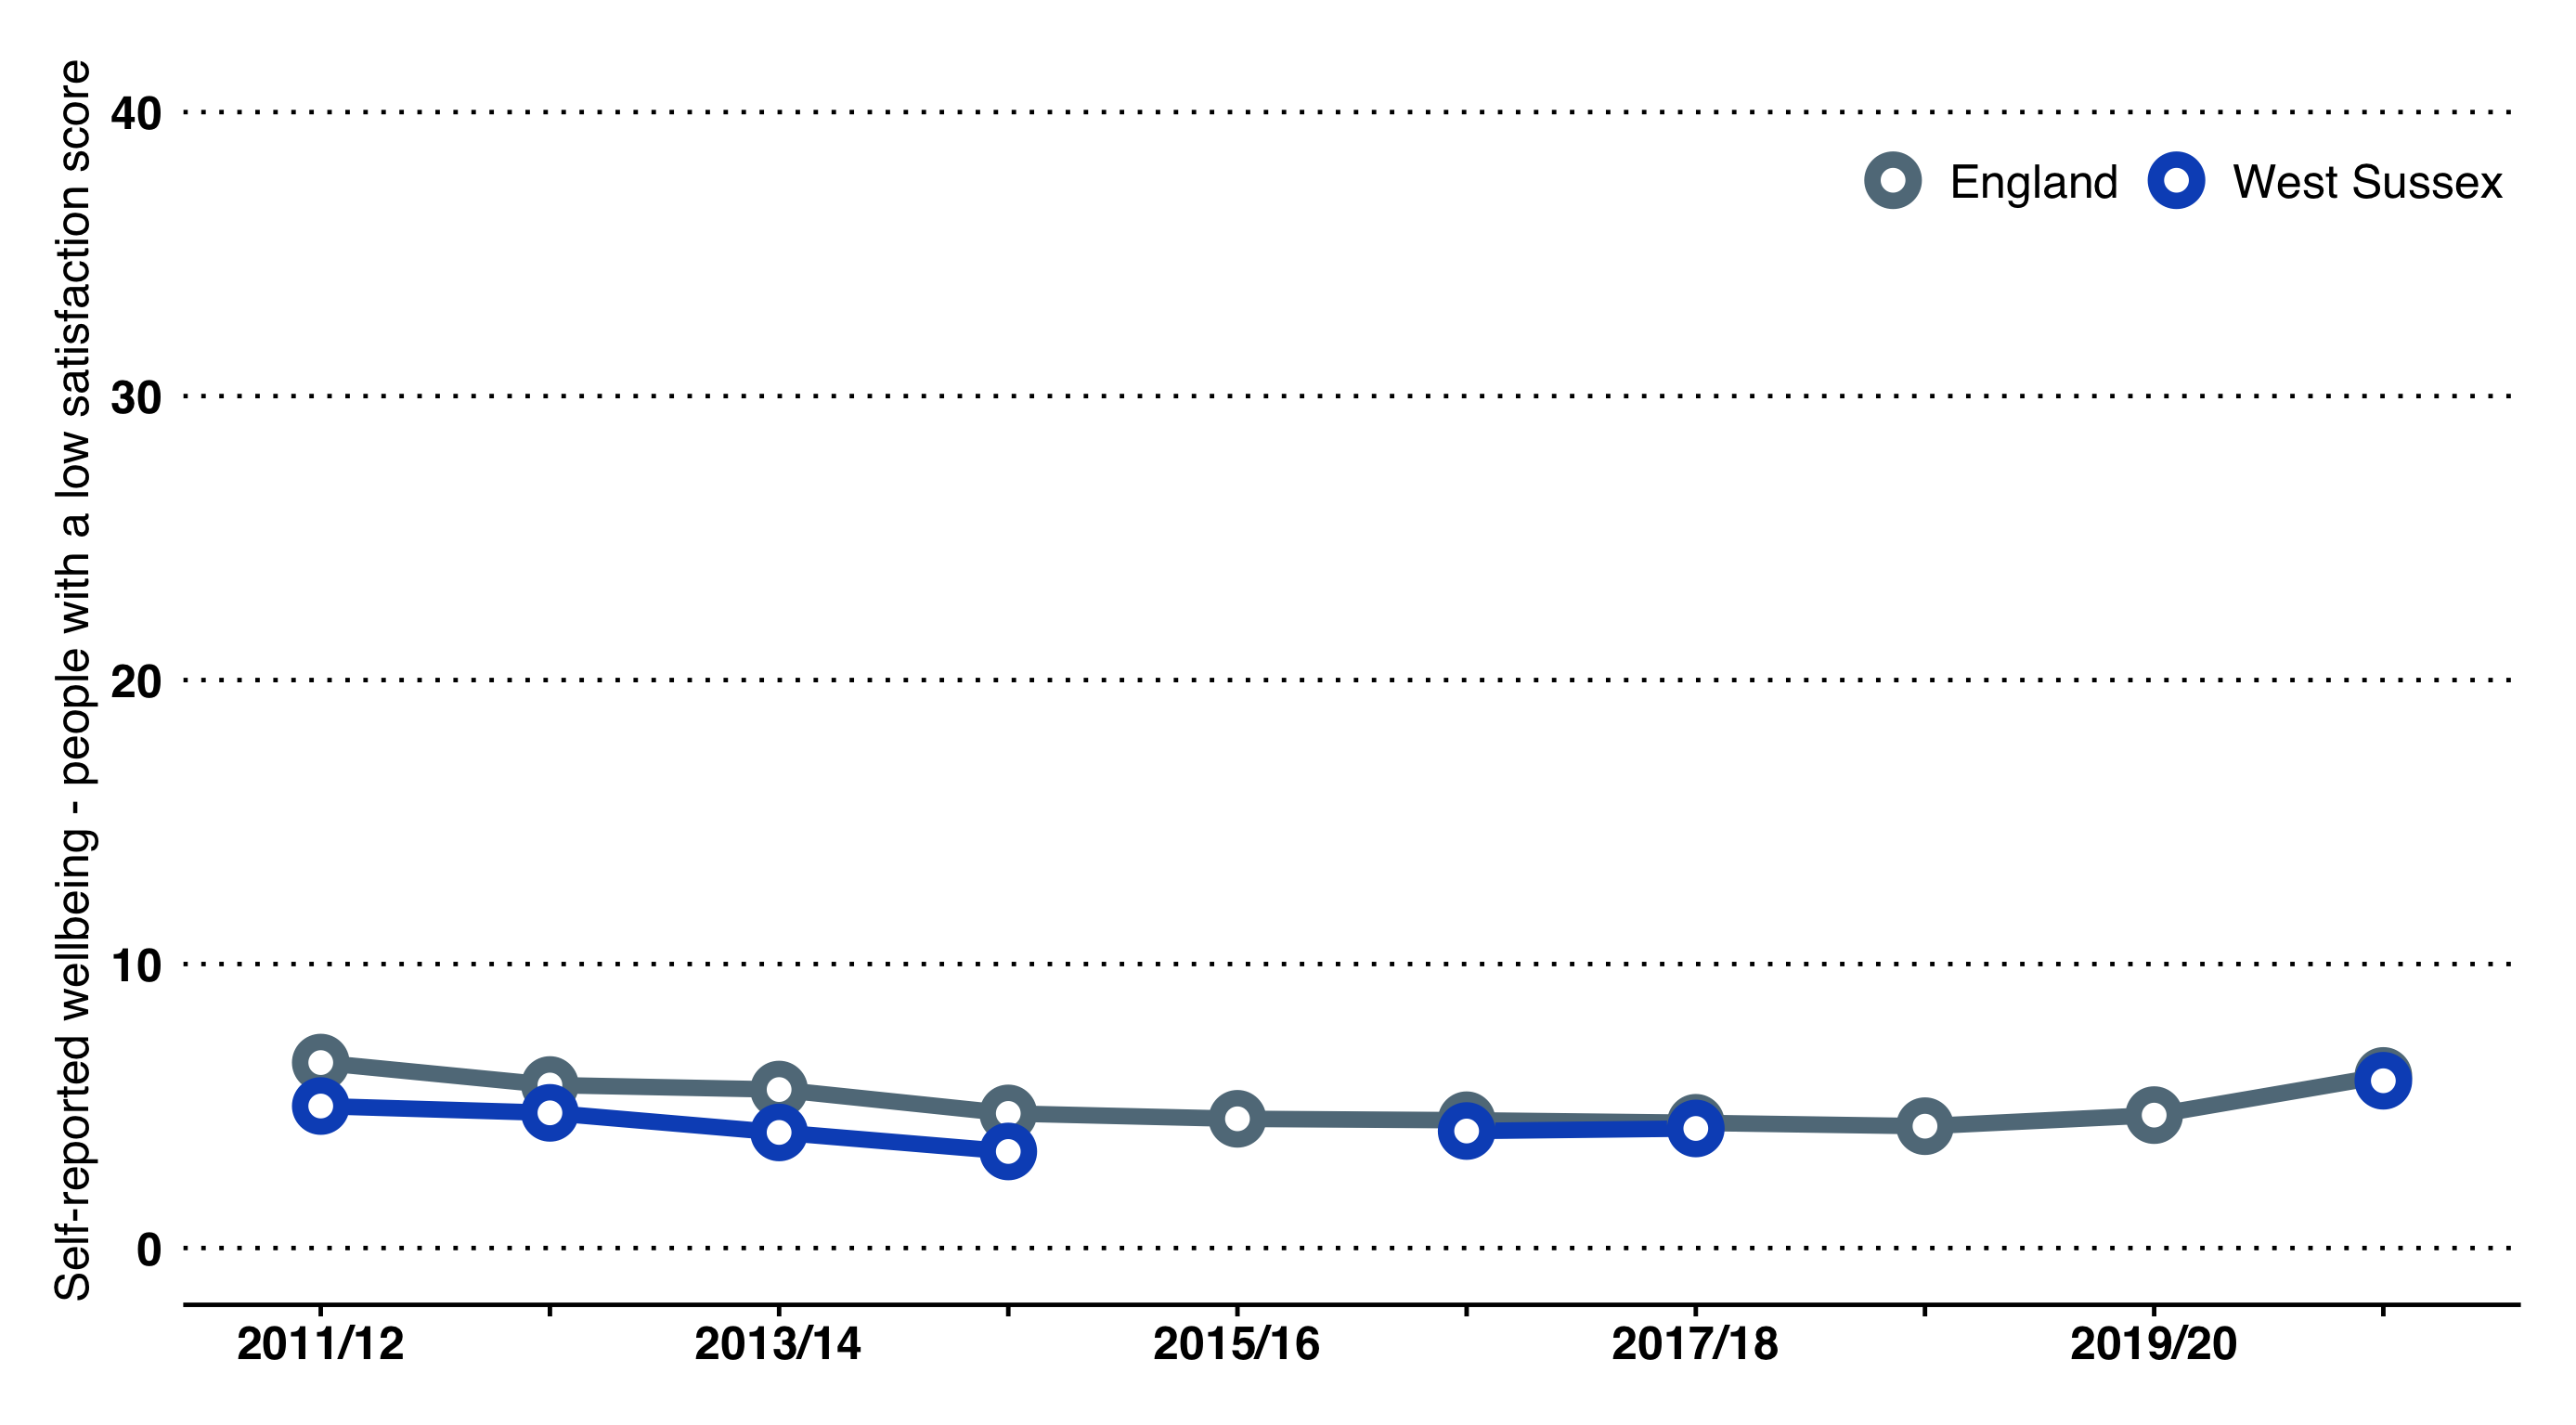
\includegraphics[width=\textwidth]{images/low_satisfaction_line.png}
    \end{subfigure}
    \begin{subfigure}[b]{0.48\textwidth}
        \centering
        \caption{People with a low worthwhile score}\label{fig:wellb-surv:loww}
        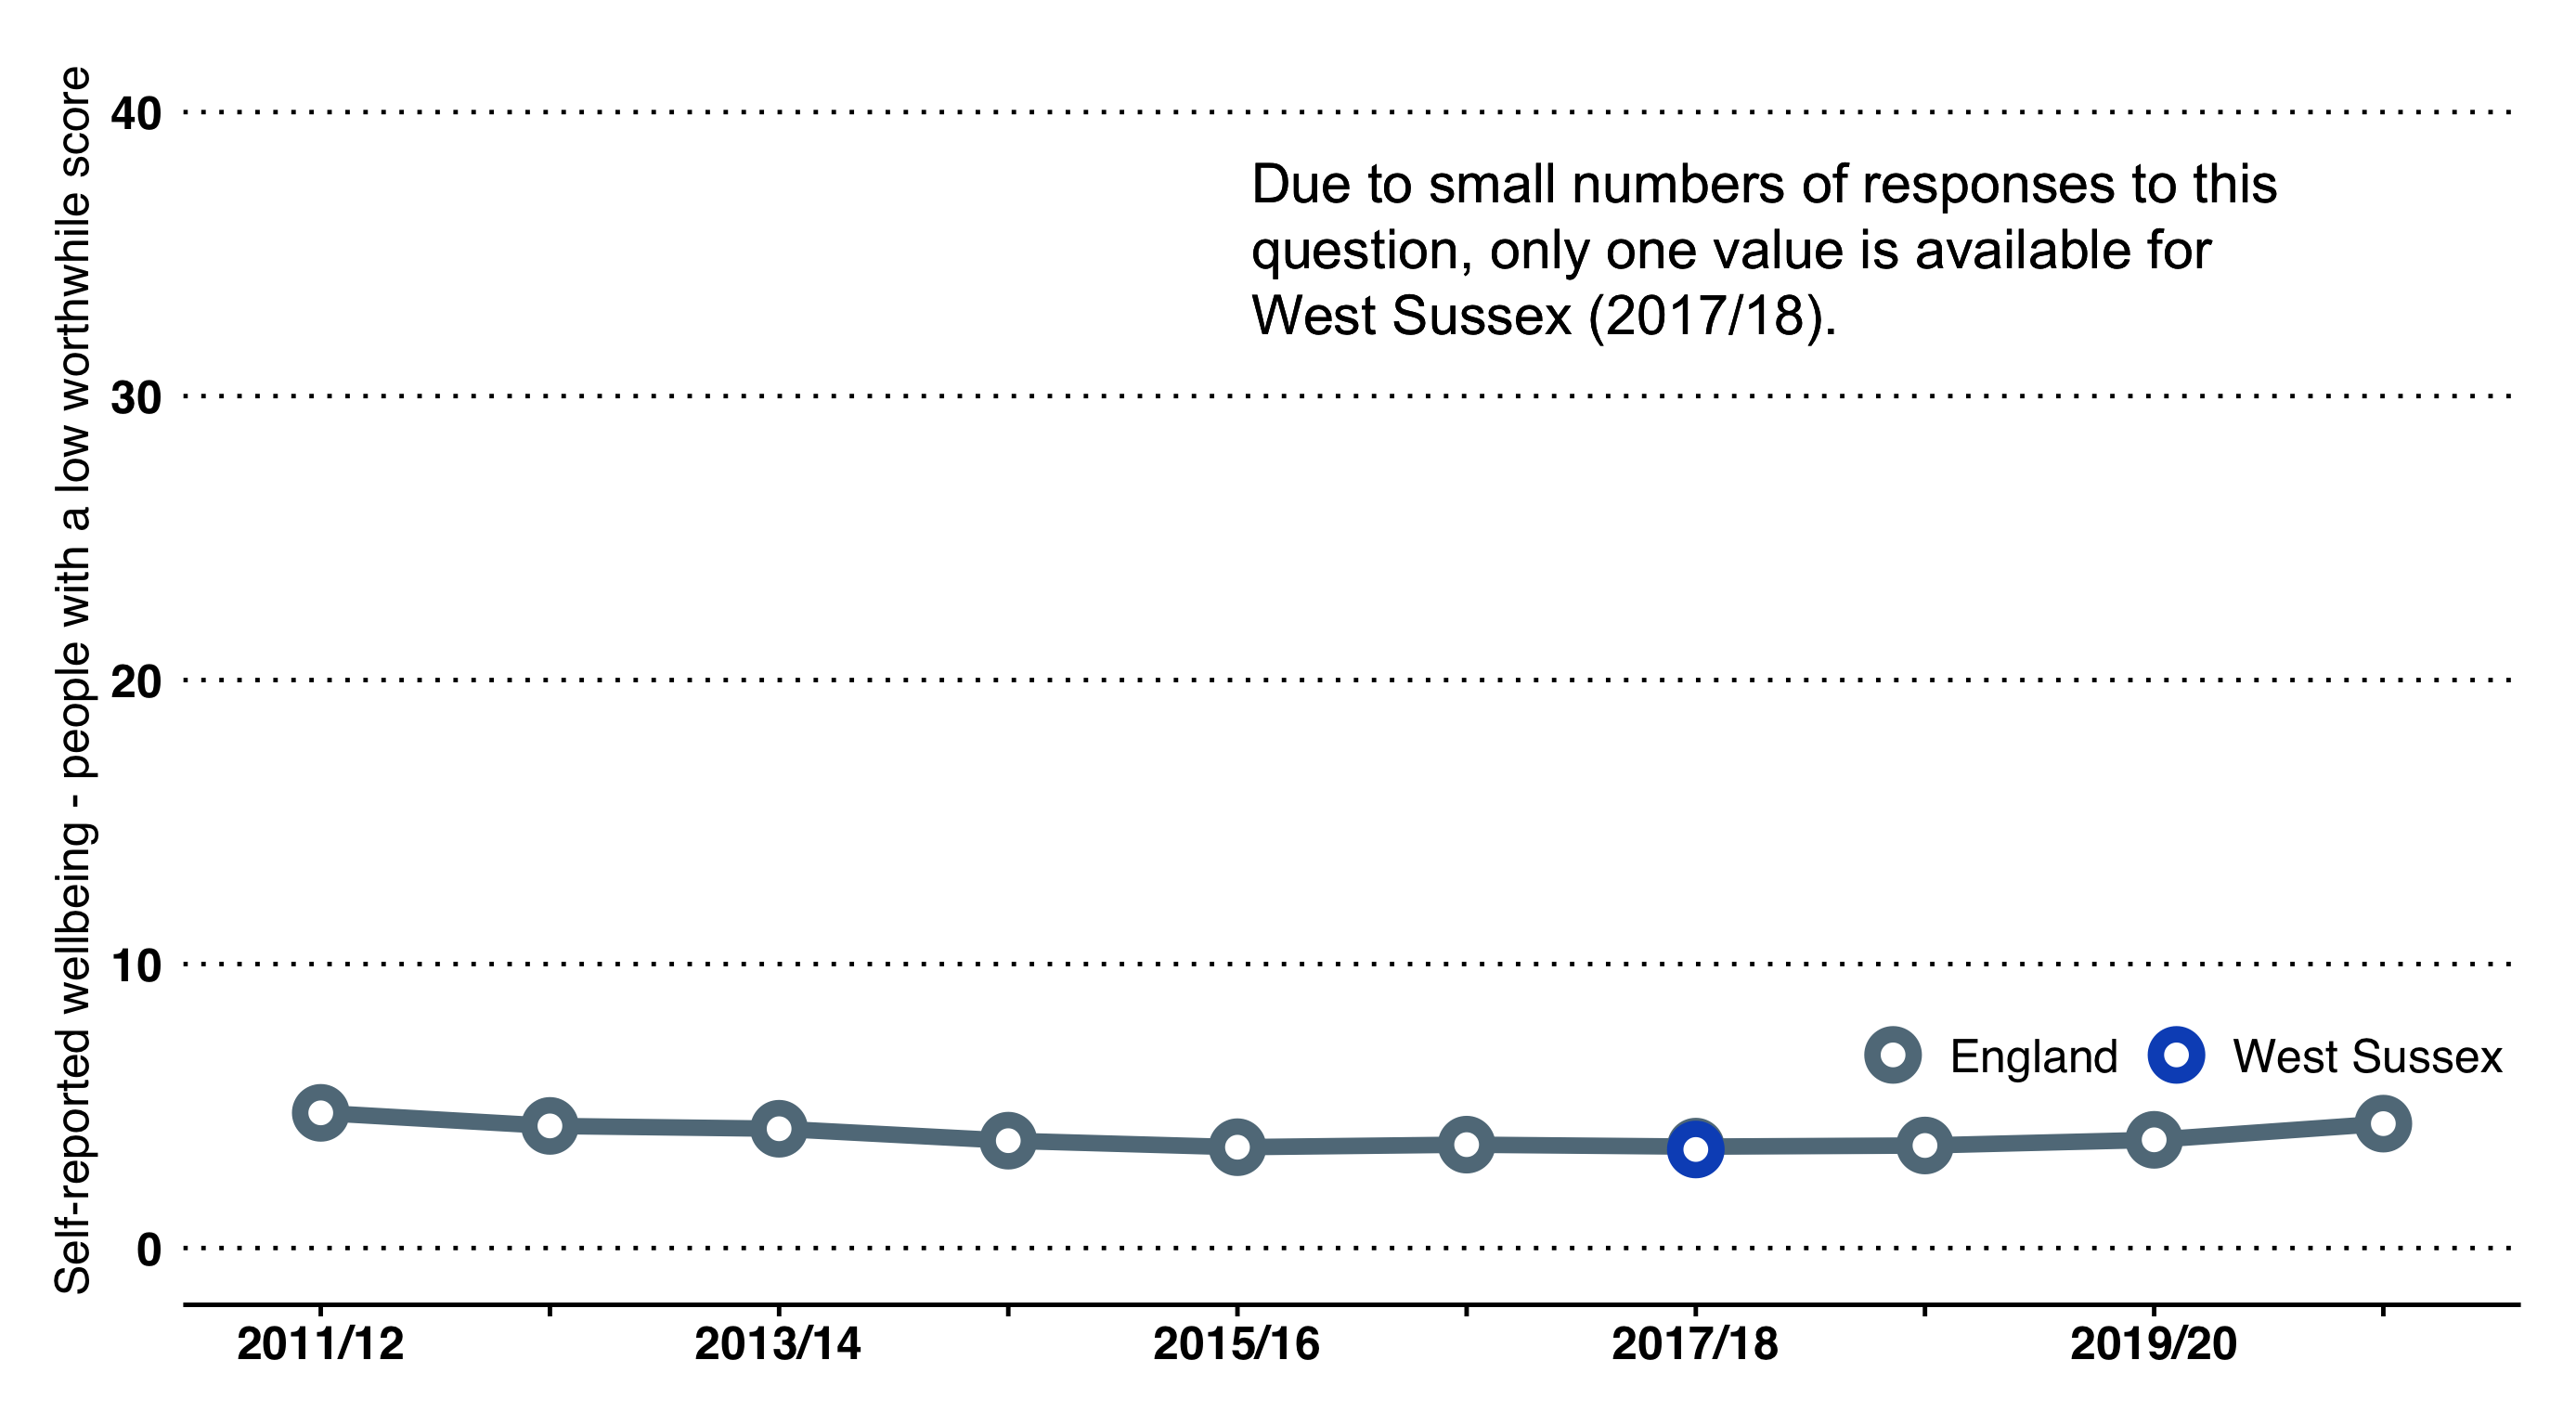
\includegraphics[width=\textwidth]{images/low_worthwhile_line.png}
    \end{subfigure}
    \vspace*{3mm}
    \begin{subfigure}[t]{0.48\textwidth}
        \centering
        \caption{People with a high anxiety score}\label{fig:wellb-surv:hanx}
        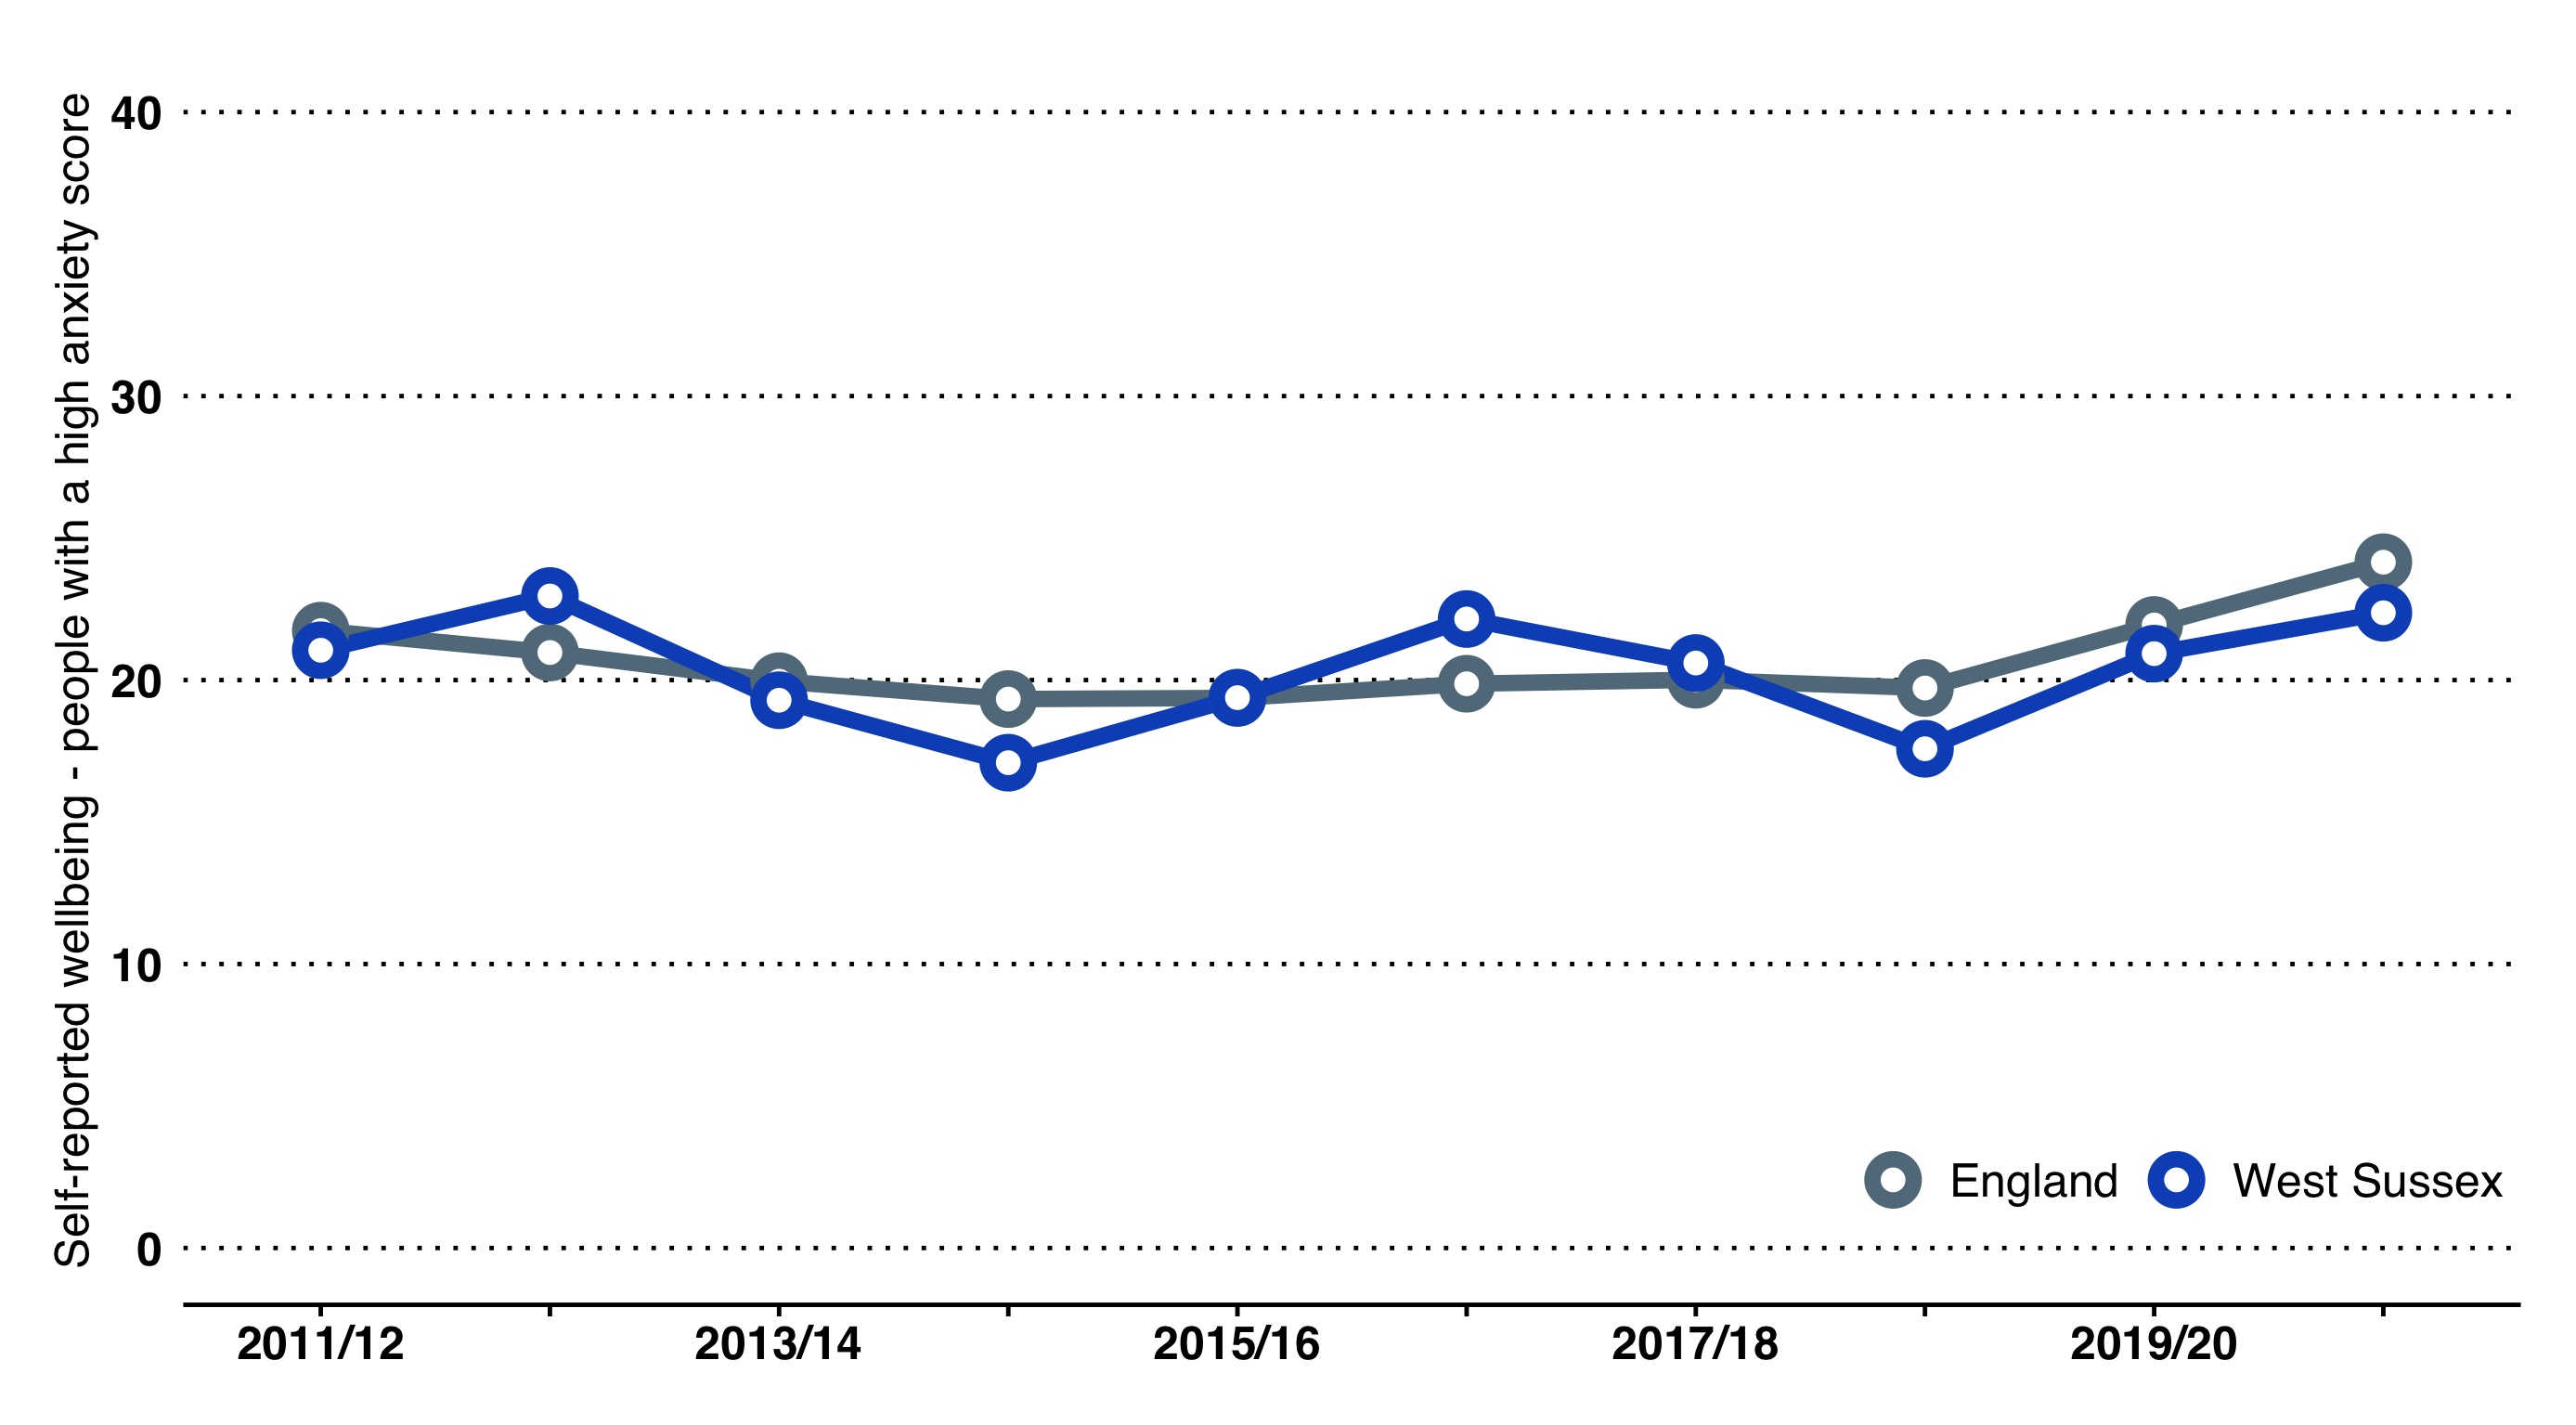
\includegraphics[width=\textwidth]{images/high_anxiety_line.png}
    \end{subfigure}
    \begin{subfigure}[t]{0.48\textwidth}
        \centering
        \caption{People with a low happiness score}\label{fig:wellb-surv:lhap}
        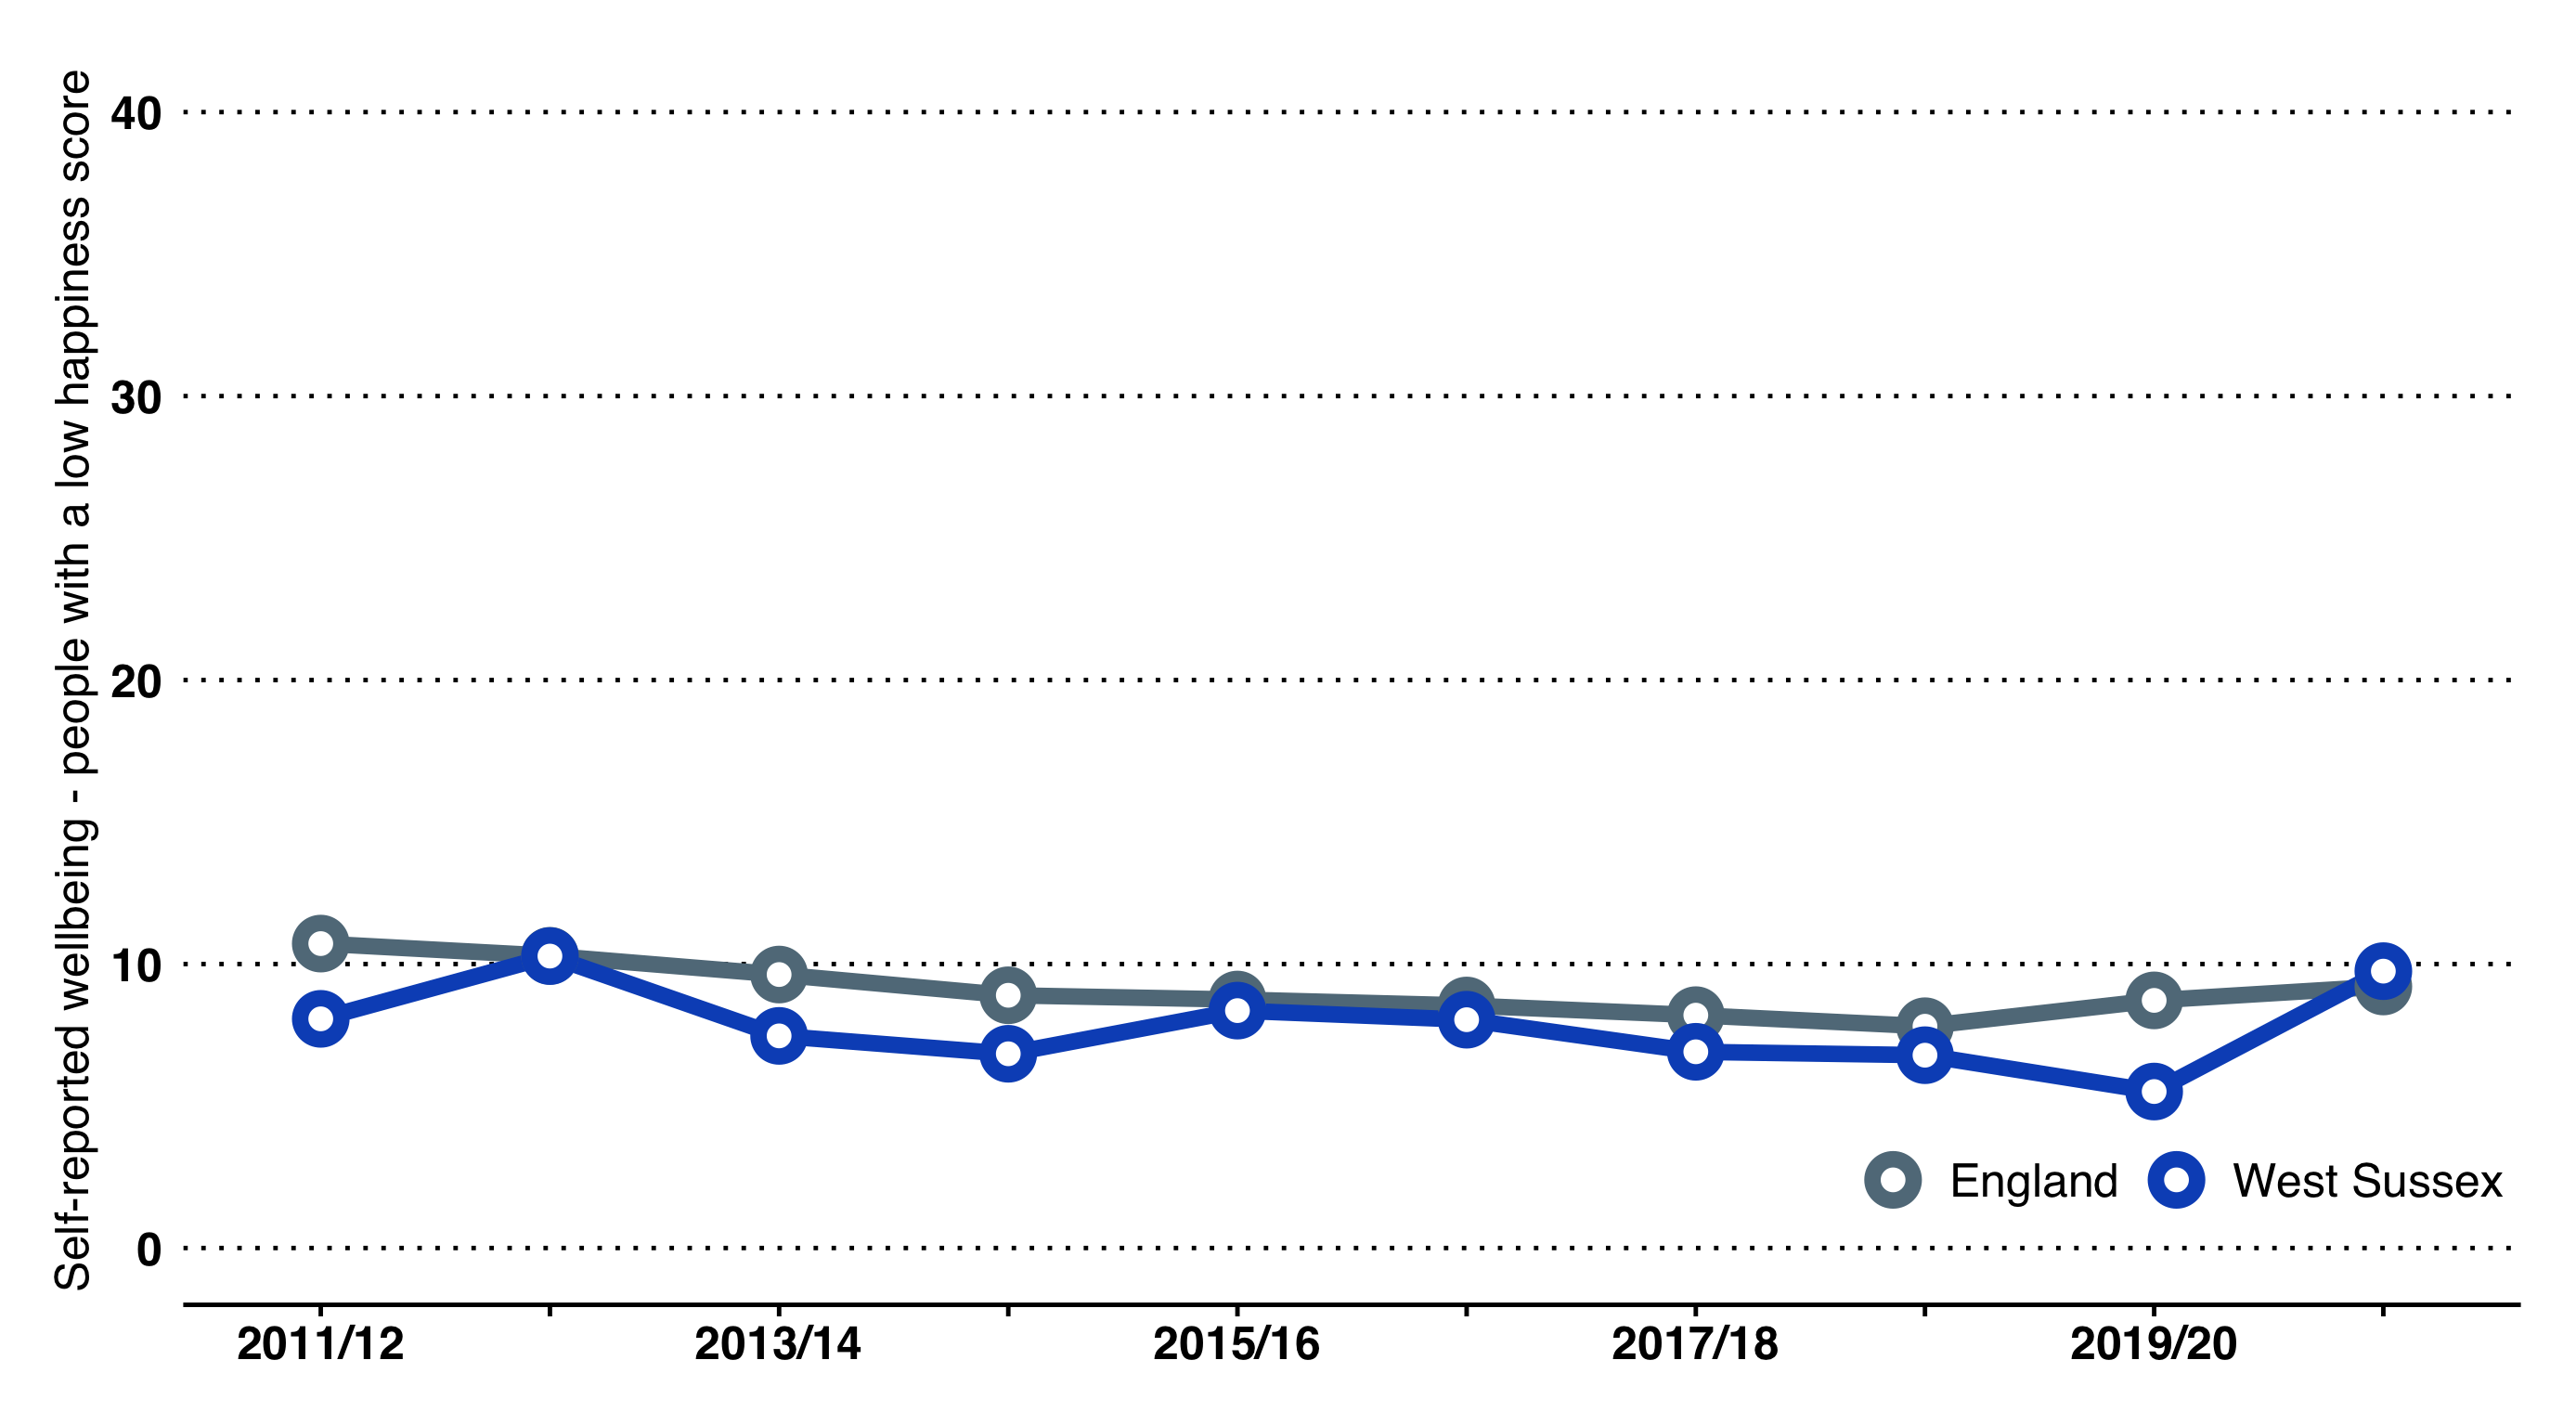
\includegraphics[width=\textwidth]{images/low_happiness_line.png}
    \end{subfigure}
\end{figure*}

\clearpage

\subsubsection{Measuring Wellbeing}
There is not a single measure of health, wellbeing or happiness: different tools focus on different things. Six commonly used tools/instruments are summarised on this page.

\begin{itemize}[noitemsep]
    \item Some tools concentrate on one domain/theme, such as health-related quality of life (HRQ0L) e.g. the EQ-5D tool.
    \item Some look at subjective wellbeing (SWB), such as the ONS Wellbeing survey.
    \item Others consider what outcomes different policy-makers are seeking answers to, such as the ability of people to undertake personal care tasks or the ability to manage a condition (e.g. self-efficacy in the Patient Activation Measure, or undertaking daily activities in adult social care surveys).
    \item Some questions focus on the frequency a feeling/experience occurs, whilst others ask about intensity (e.g. WEMWBS asks about frequency whilst ONS Wellbeing asks about intensity).
\end{itemize}

% To improve the understanding of tools available we have drafted a briefing of the main options available, which is available on the JSNA website.
% For further information please contact Clare Toon (\url{clare.toon@westsussex.gov.uk}) or Jacqueline Clay (\url{jacqueline.clay@westsussex.gov.uk}).

\begin{tcolorbox}[colback={boxcolour}, title={ONS Subjective Wellbeing}]
    Subjective wellbeing, designed as an adjunct to GDP measurement at a national level. Questions include evaluation, eudemonic and experience approaches.
    
    {\bf Pros:} Short, used widely. Nationally developed measure can be applied across programmes.
    
    {\bf Cons:} Not specifically centred on health, but broader subjective wellbeing. May not be sensitive to short term change
\end{tcolorbox}

\begin{tcolorbox}[colback={boxcolour},title={WEMWBS / Warwick Edinburgh}]
    Warwick Edinburgh Mental Wellbeing Measure, focuses on mental health and wellbeing and has a long and short version.

    {\bf Pros:} Widely used, long and short versions. Sums to provide a composite score, which can be useful in dissemination.

    {\bf Cons:} Centred on individual, using only positive statements. Scale relatively short, may not pick up small movement. In a recent local evaluation there were some problems reported in using with the very elderly (85+ years).
\end{tcolorbox}

\begin{tcolorbox}[colback={boxcolour},title={Outcomes Stars (wide range)}]
    Concentrates on using a specific format (spider diagram) and a wide range of measures for different groups and contexts within the population (e.g. young people, family, carers, homelessness)

    {\bf Pros:} Wide range of tools may be more suitable for specific conditions and circumstances, although less suitable for overall strategic reporting. Good visual format, easy to undertake

    {\bf Cons:} To use this tool an annual fee is paid (not prohibitive approx. £350)
\end{tcolorbox}

\begin{tcolorbox}[colback={boxcolour},title={Patient Activation Measure (PAM)}]
    Self-efficacy, willingness and ability to take on role of managing own health and health conditions. Describes activation in 4 levels (low activation to having the skills to self-manage)

    {\bf Pros:} Measures the ability of self-efficacy; the value is in understanding a patient's ability and starting point. Can be used across programmes.

    {\bf Cons:} Does not focus on issues of wider wellbeing. Fluctuates with deterioration, not necessarily linear assumption and not designed to be a high level performance measure. Costs (but not prohibitive)
\end{tcolorbox}

\begin{tcolorbox}[colback={boxcolour},title={EQ-5D}]
    Developed by the EuroQol Group as a measure of health-related quality of life. Widely used, has some overlap with ASCOF. Measure of intensity. Has a 3 level range version and a 5 level version
    
    {\bf Pros:} Widely used in health, wide application possible Easy, simple questions. Used for economic evaluation
    
    {\bf Cons:} Narrow view of health-related quality of life does not cover more subjective aspects of wellbeing. Requires registration but cost minimal.
\end{tcolorbox}

\begin{tcolorbox}[colback={boxcolour},title={ASCOF}]
    Measures social-care related quality of life - developed to assess whether a person's social care needs and wants are being met.
    
    {\bf Pros:} Validated and used annually by council (only with people in receipt of services). Would be expected to decline with increased age and frailty, if population frame altered (i.e. fewer, frailer people accessing care). Useful range of tools for format (self- complete/proxy), easy read
    
    {\bf Cons:} Narrow focus. Designed for a specific function/policy area.
\end{tcolorbox}

\subsection{Premature Mortality}
\begin{figure}[htp]
    \caption[Age-standardised mortality rate (under 75 years) - Cardiovascular diseases]{Age-standardised mortality rate (under 75 years) - Cardiovascular diseases}
    \centering
    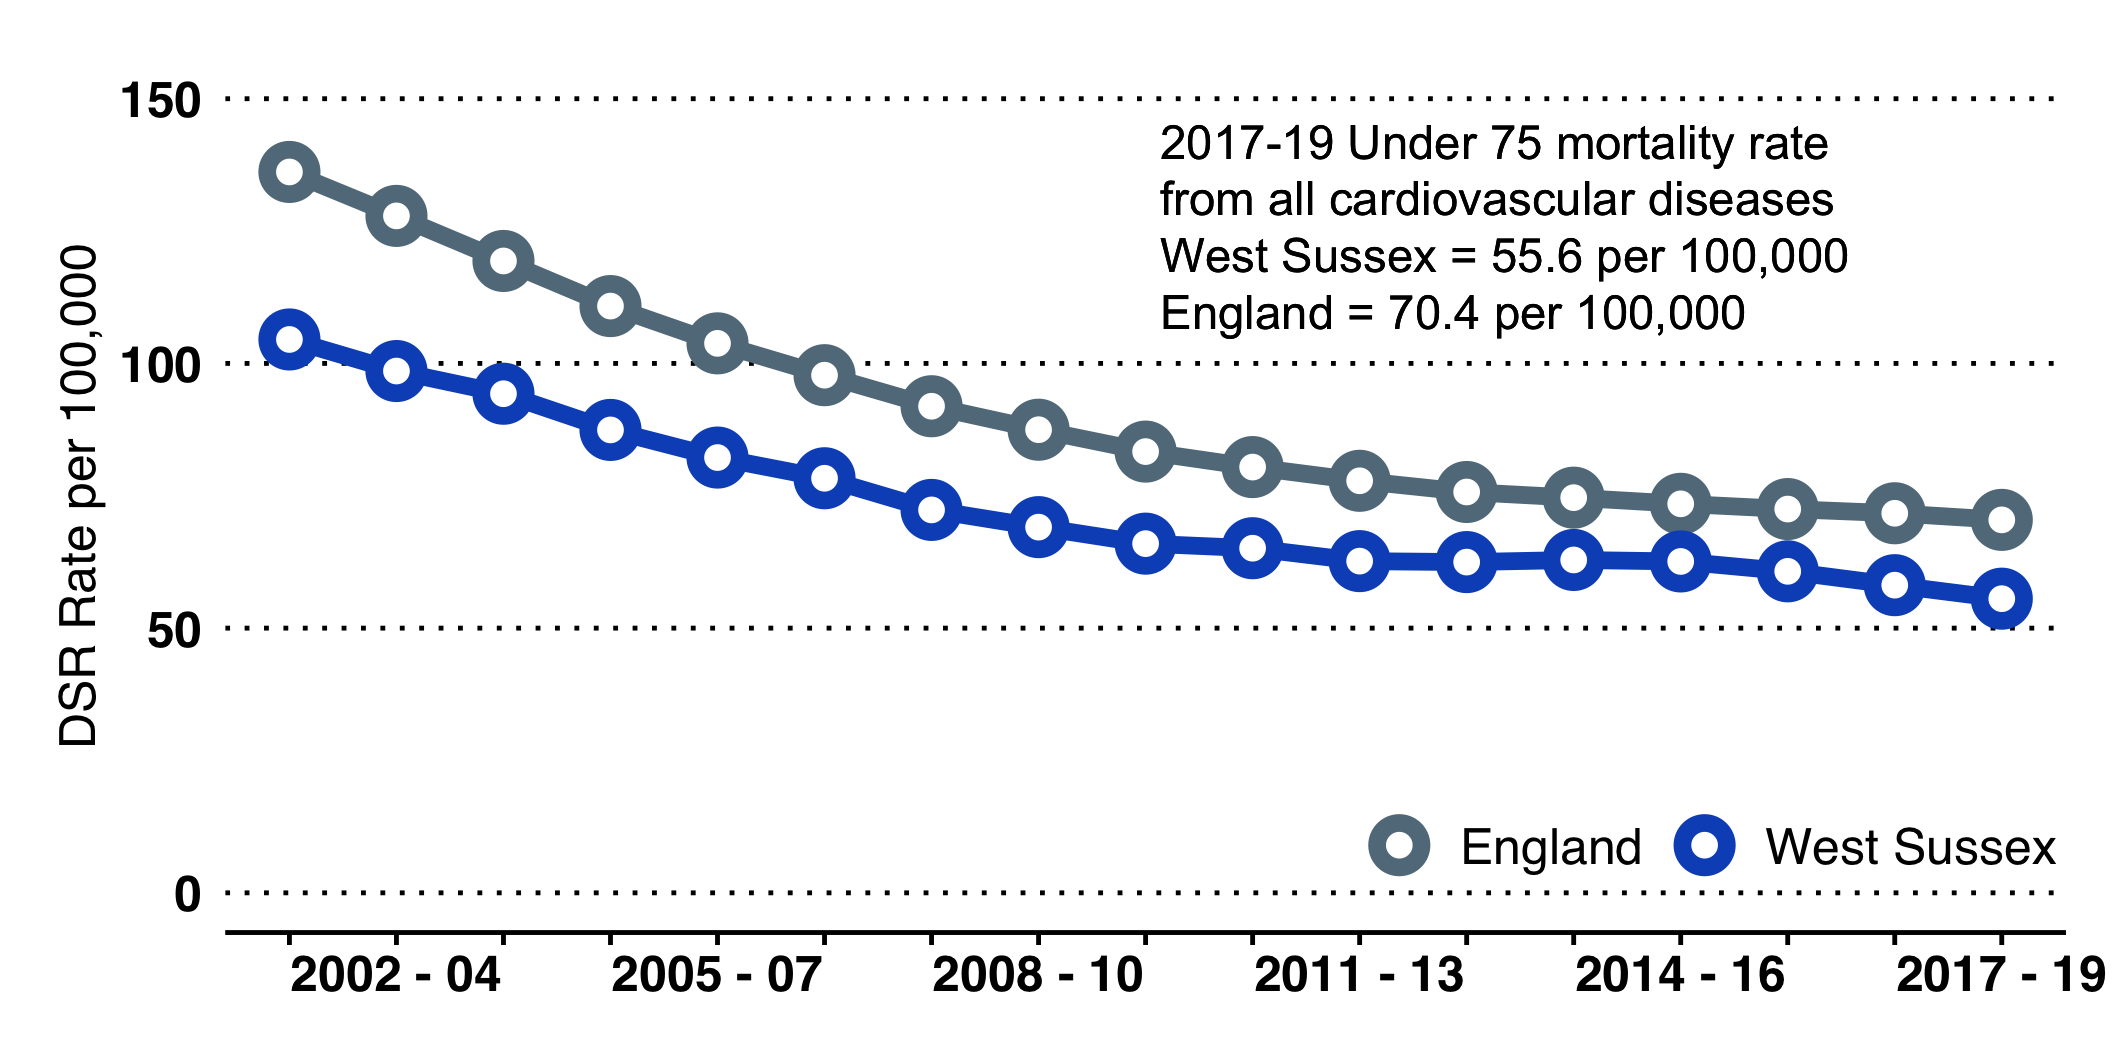
\includegraphics[width=.95\linewidth]{images/u75_cvd_line_3y.png}
    \label{fig:u75_cvd}
\end{figure}

Cardiovascular disease (CVD) remains a major cause of premature mortality. The rate has reduced greatly over the last 20 years, due to lifestyle improvement and treatment. The mortality rate in West Sussex is significantly better than the England rate\footnote{PHOF reference E04a}. 

\begin{figure}[htp]
    \caption[Age-standardised mortality rate (under 75 years) - Cancer]{Age-standardised mortality rate (under 75 years) - Cancer}
    \centering
    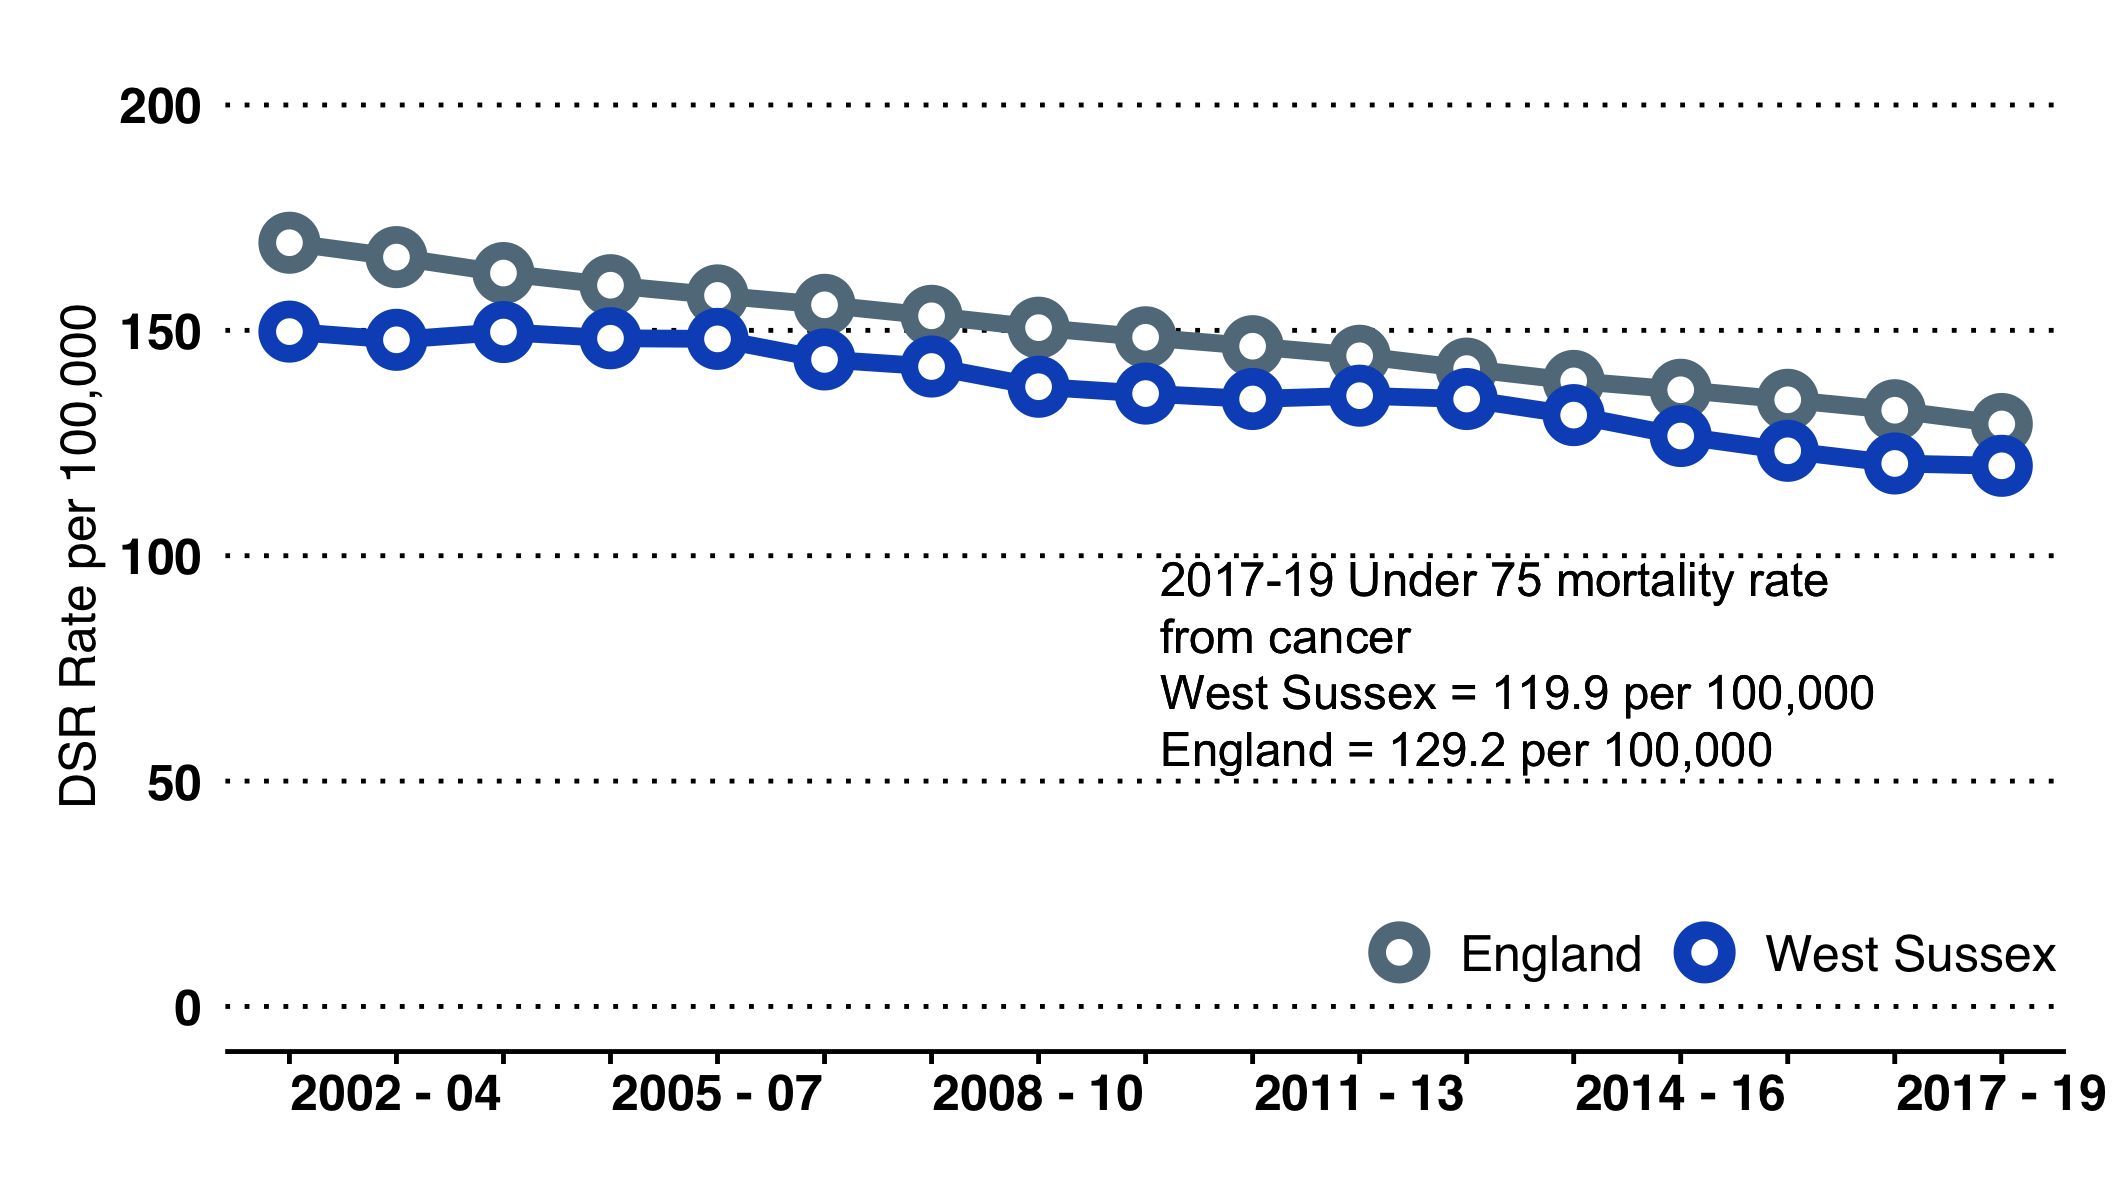
\includegraphics[width=.95\linewidth]{images/u75_cancer_line_3y.png}
    \label{fig:u75_cancer}
\end{figure}

Cancer remains the biggest cause of death for people under 75. A continued reduction will require sustained effort on prevention, early diagnosis and treatment. The rate in West Sussex is significantly better than the England rate\footnote{PHOF reference E05a}.

\begin{figure}[htp]
    \caption[Age-standardised mortality rate (under 75 years) - Liver Disease]{Age-standardised mortality rate (under 75 years) - Liver Disease}
    \centering
    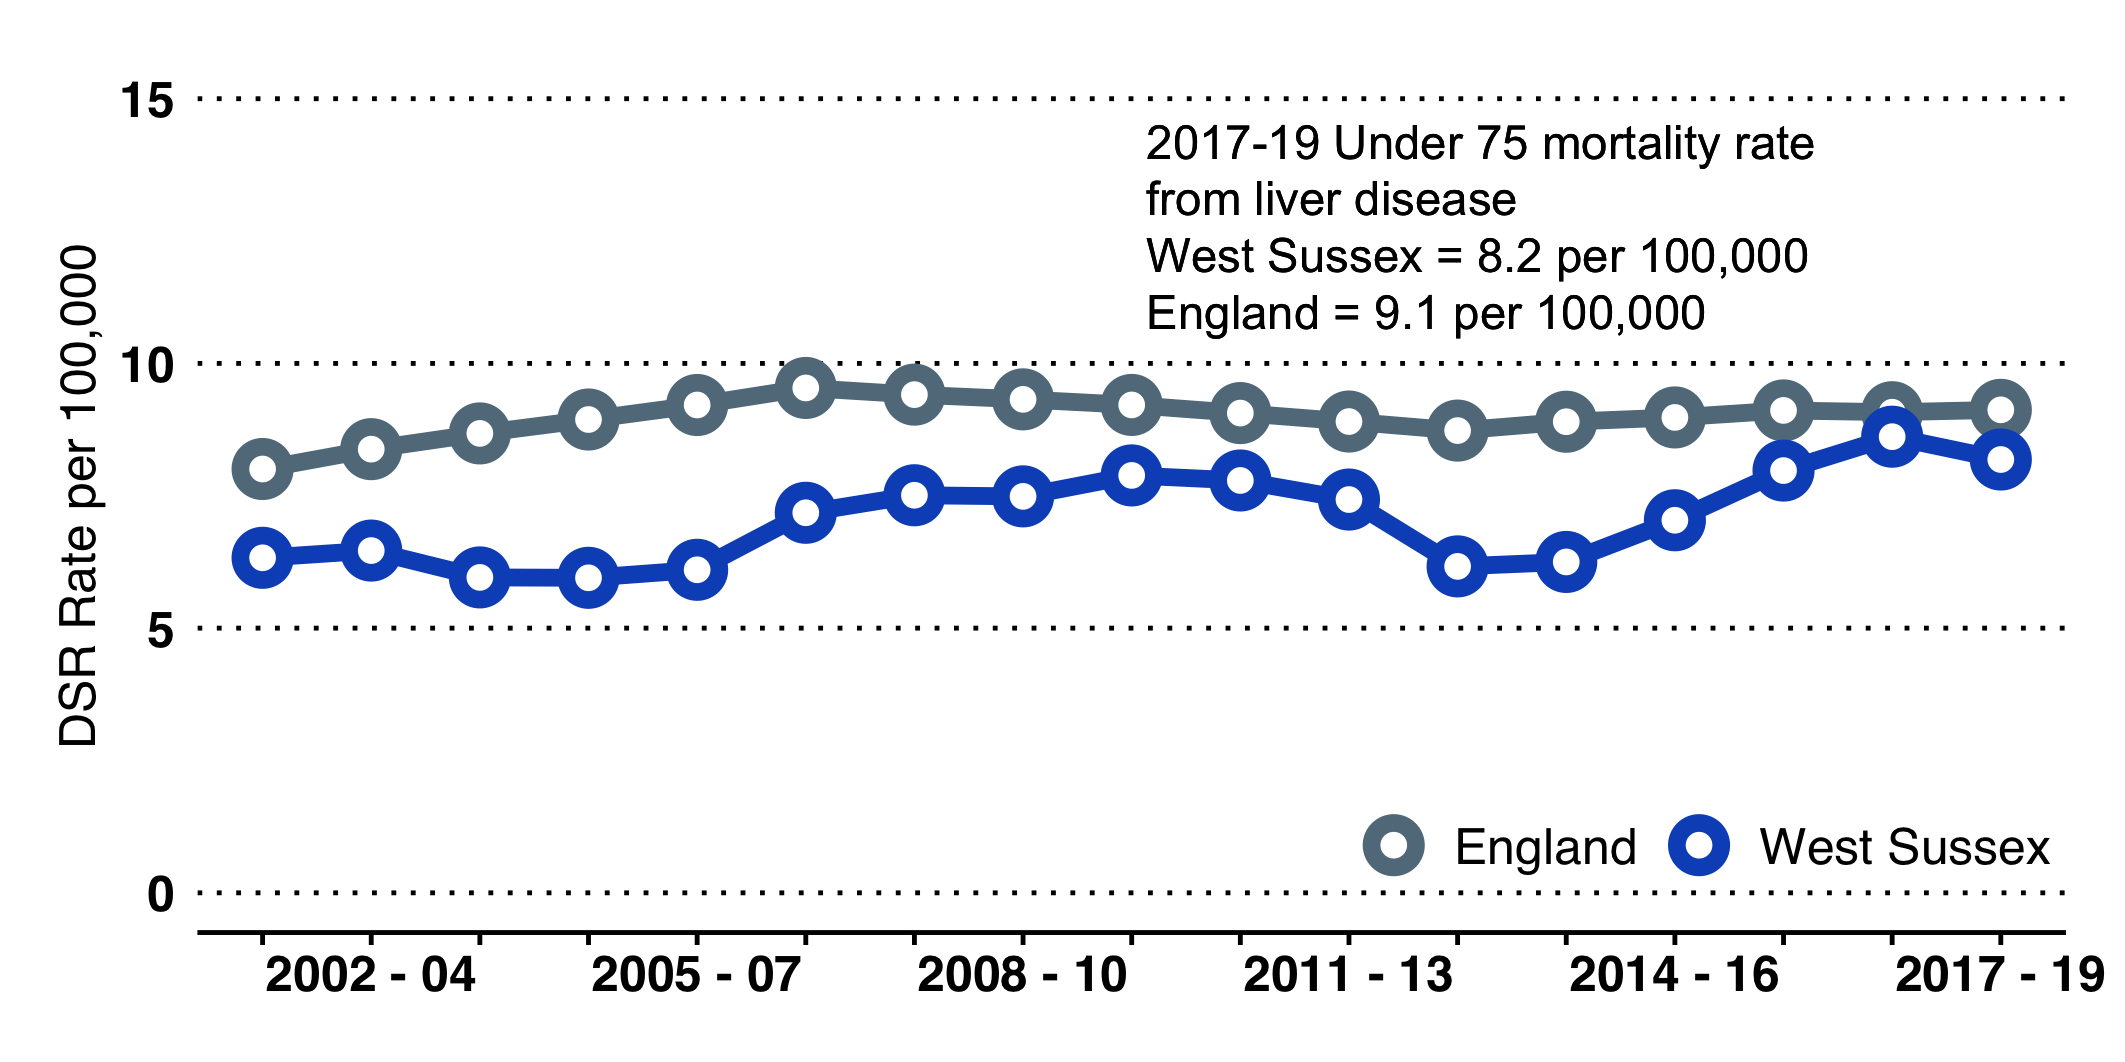
\includegraphics[width=.95\linewidth]{images/u75_liver_line_3y.png}
    \label{fig:u75_liver_b}
\end{figure}

Liver disease is a major cause of premature death. Most liver disease is preventable; both alcohol consumption and obesity are underlying factors, amenable to public health interventions. Of the major causes, the rate of mortality is not reducing. Locally the rate is below England\footnote{PHOF reference E06a}. 

\begin{figure}[htp]
    \caption[Age-standardised mortality rate (under 75 years) - Respiratory Disease]{Age-standardised mortality rate (under 75 years) - Respiratory Disease}
    \centering
    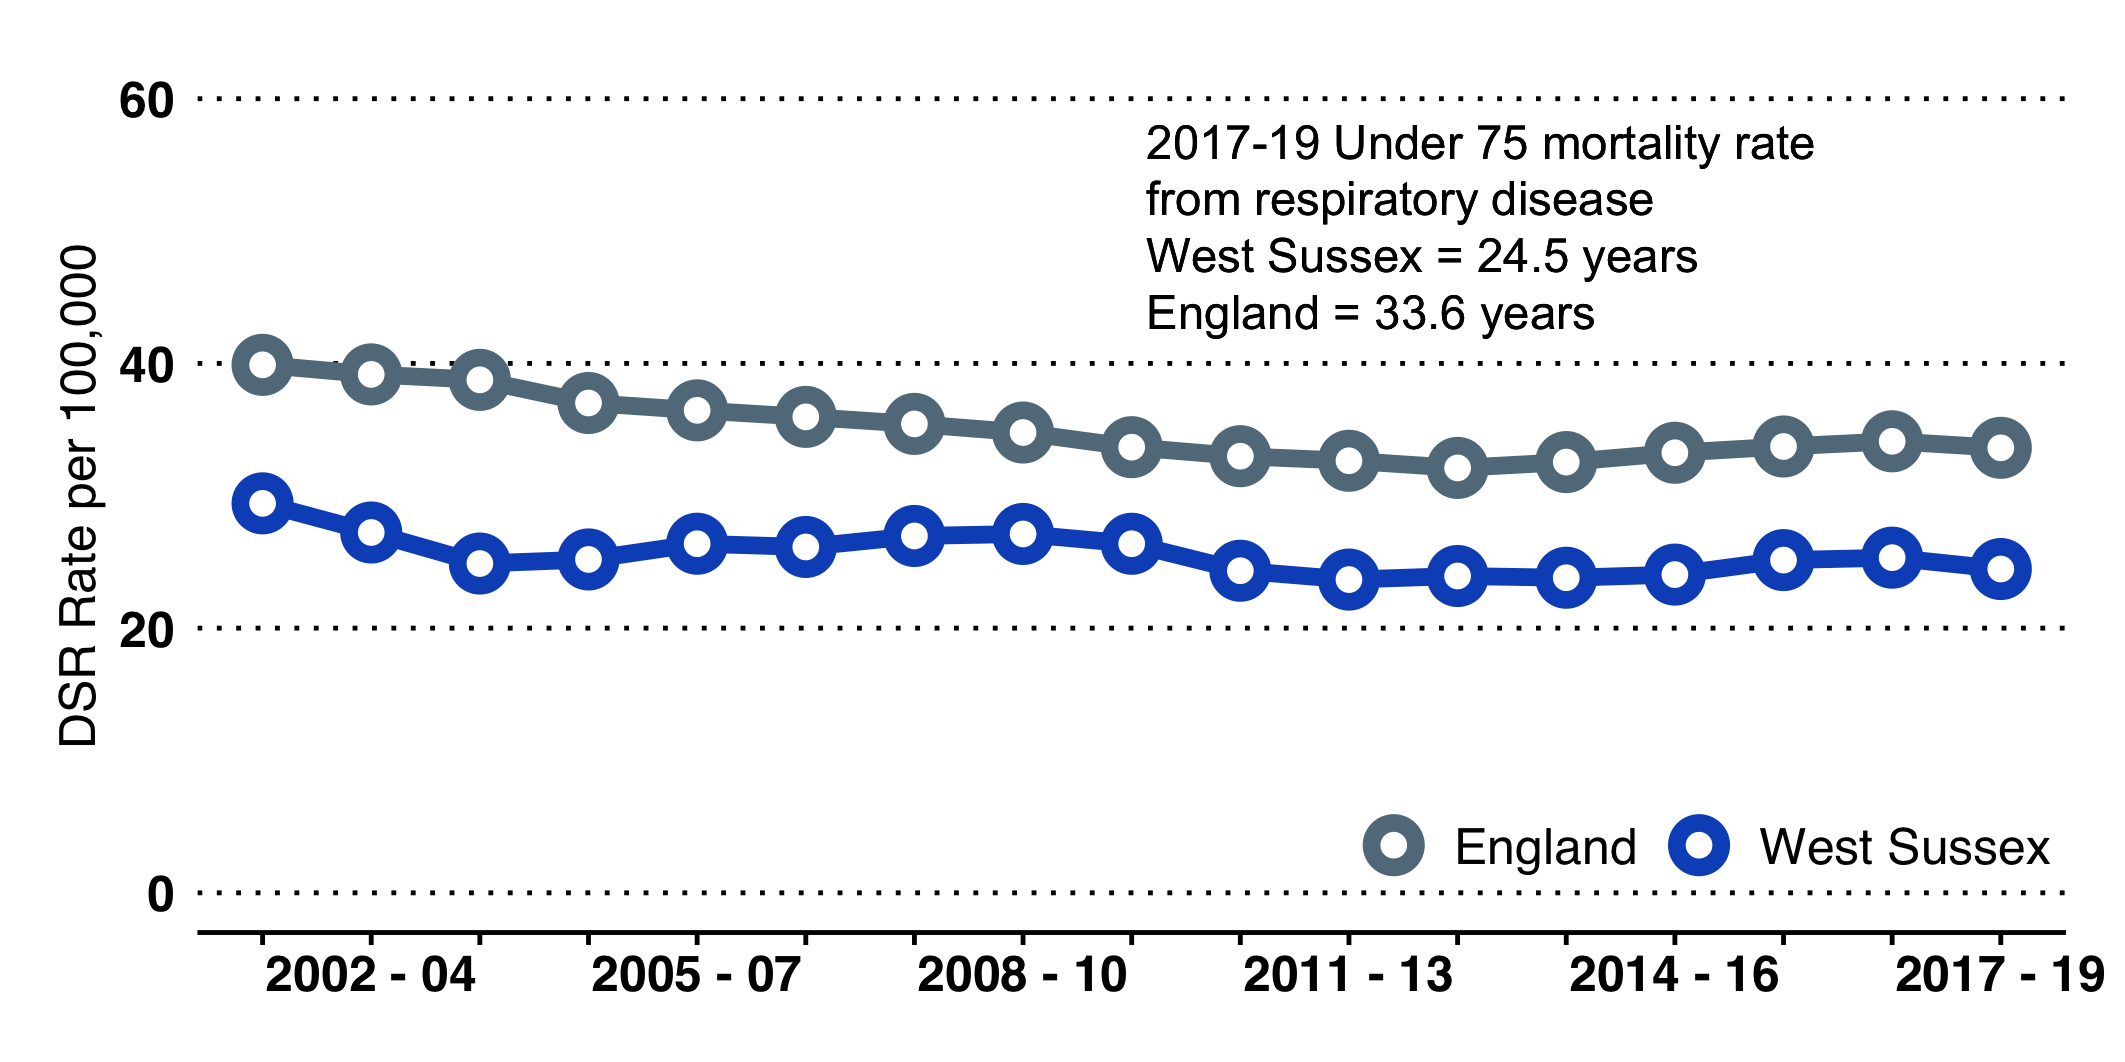
\includegraphics[width=.95\linewidth]{images/u75_respiratory_line_3y.png}
    \label{fig:u75_resp}
\end{figure}

Respiratory disease is a major cause of premature mortality. For chronic obstructive pulmonary disease (COPD), one of the main respiratory diseases, smoking is a major cause. The West Sussex rate is below that of England\footnote{PHOF reference E07a}.

\subsection{Suicide}
The West Sussex Public Health and Social Research Unit carried out a Suicide Audit in 2017, covering suicides in the years 2013 to 2015. The audit provided detailed background context and circumstances and was undertaken to inform the local Suicide Prevention Strategy.

\begin{figure}[htp]
    \caption[Age-standardised mortality rate from suicide and injury of undetermined intent per 100,000 population (all ages) over time]{Age-standardised mortality rate from suicide and injury of undetermined intent per 100,000 population (all ages) over time\footnote{PHOF reference E10}.}
    \centering
    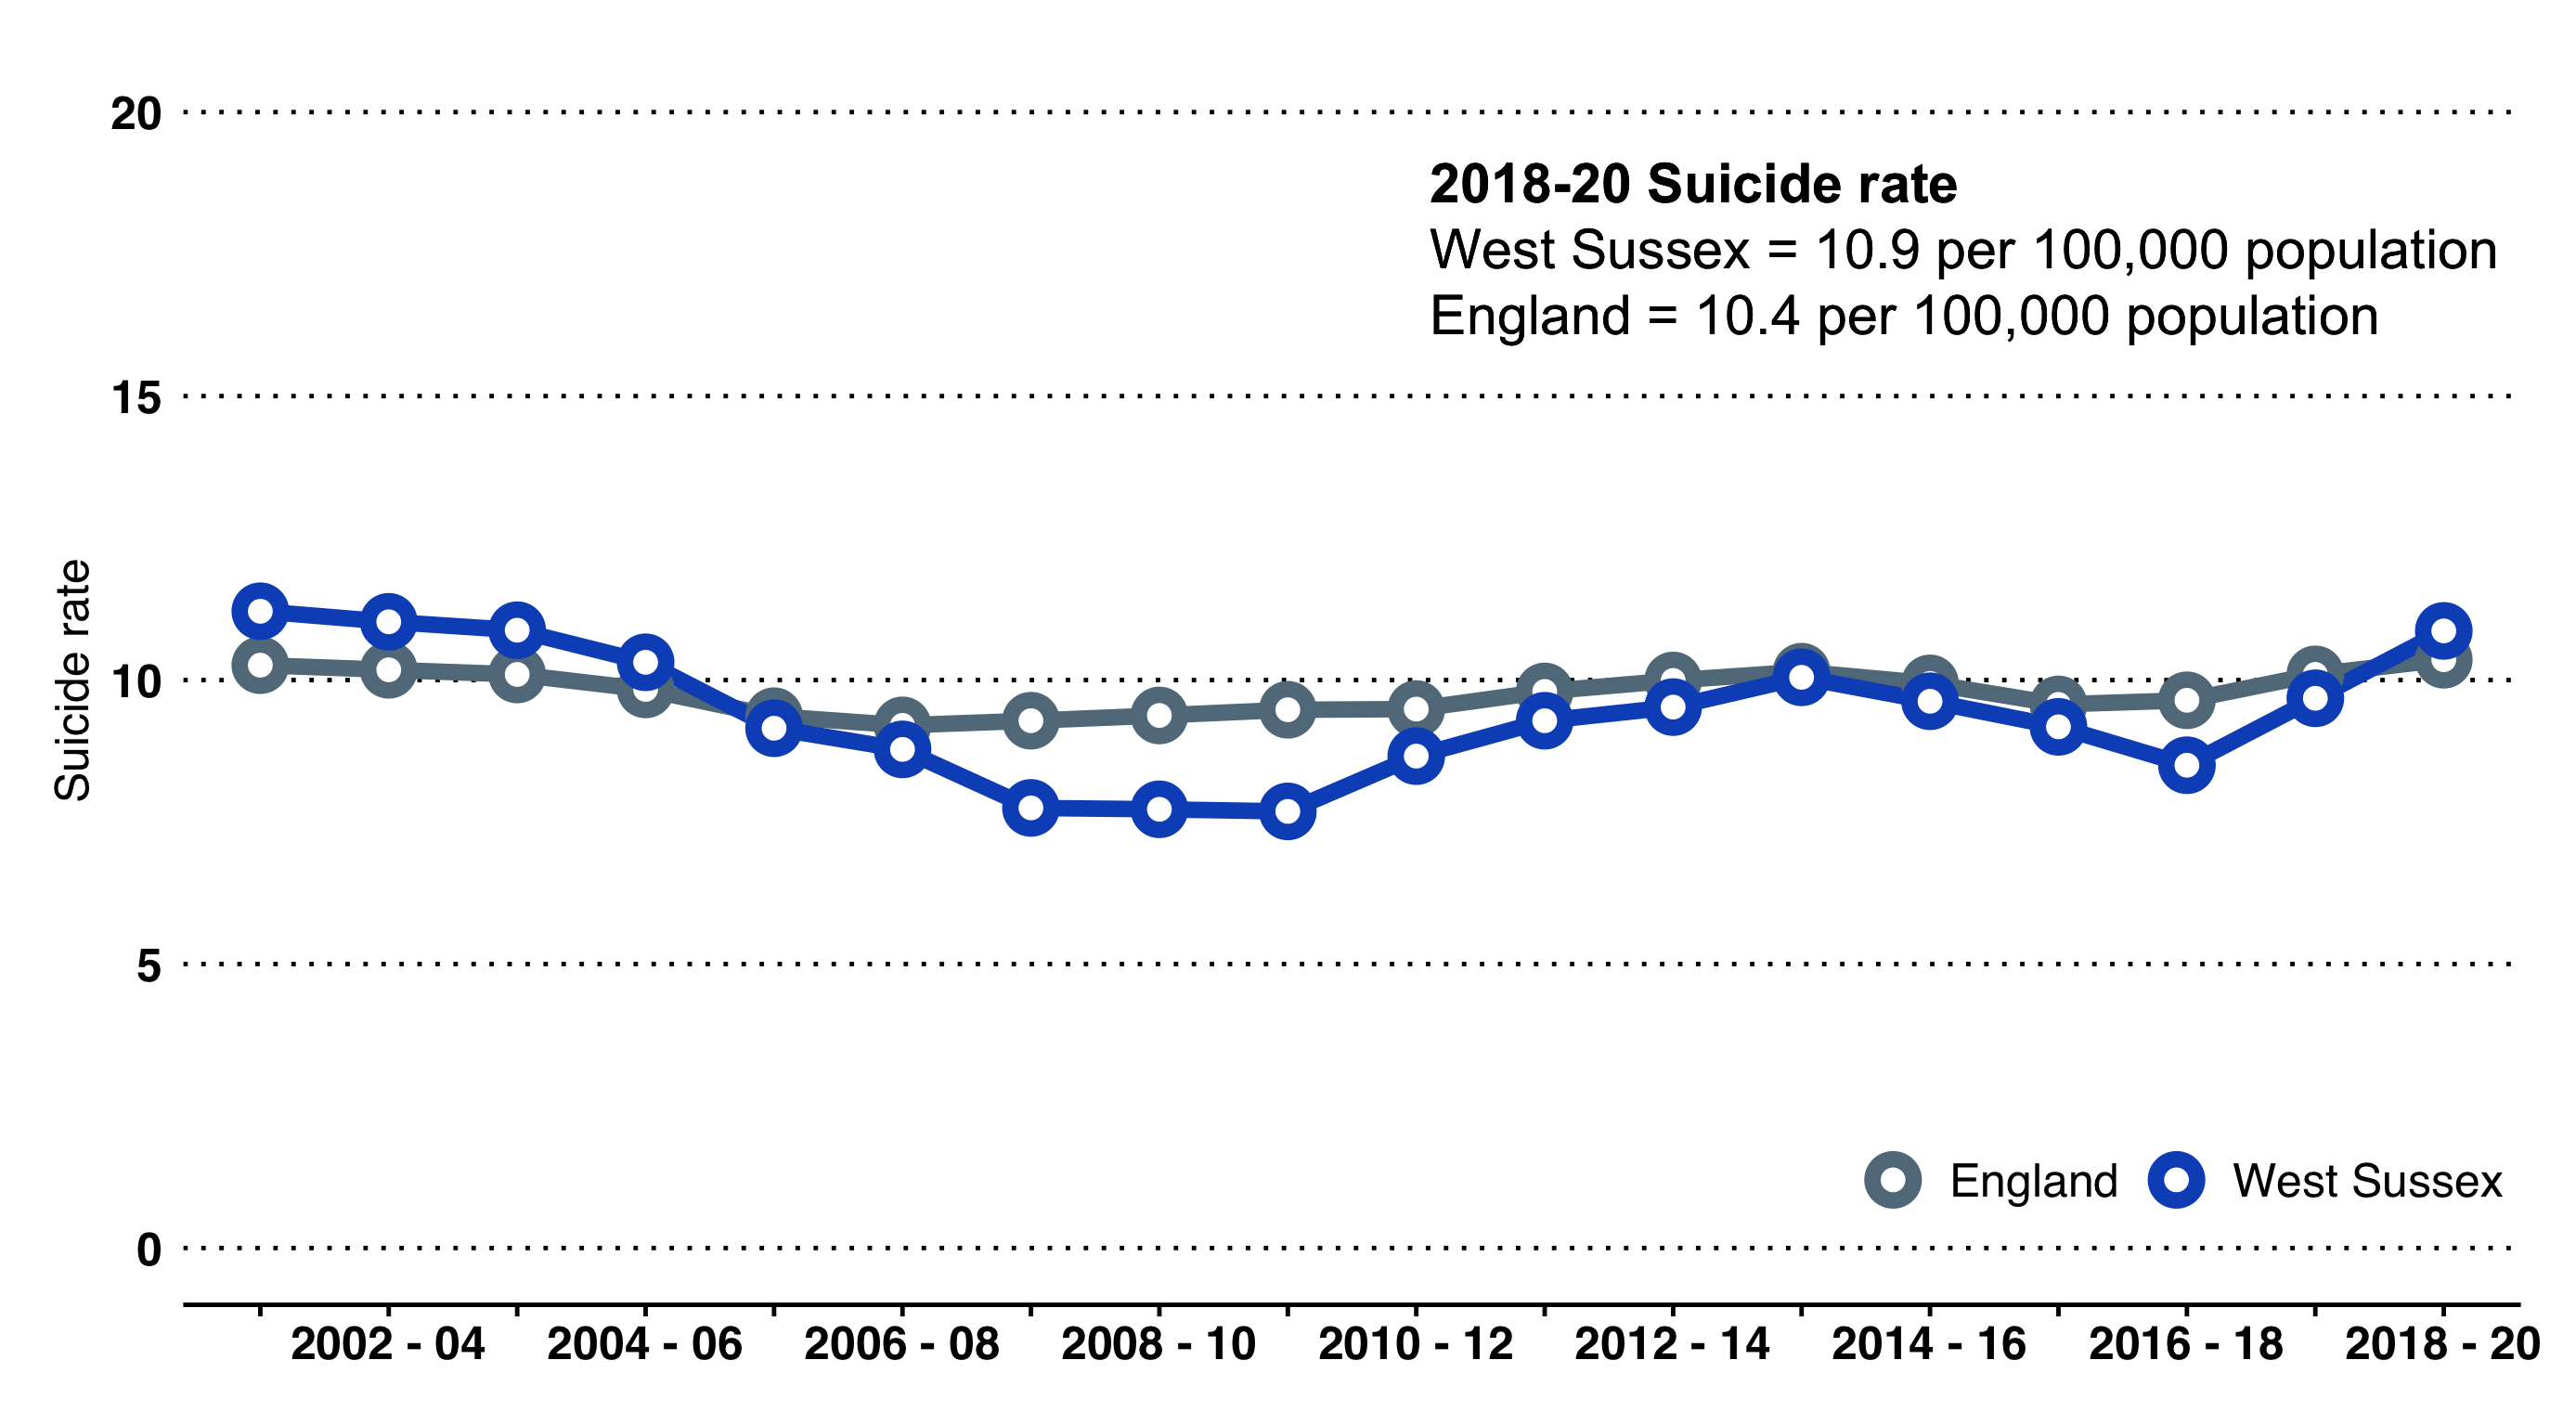
\includegraphics[width=\linewidth]{images/suicide_line.png}
    \label{fig:suicide}
\end{figure}

\subsubsection{Demographic Information from the West Sussex Suicide Audit 2013-15} For the years 2013-15 inclusive, there were 190 confirmed suicides and 23 open verdicts likely to be suicides.
\begin{itemize}[noitemsep]
    \item Combined, there were 52 females and 161 males included in the audit.
    \item Seasonal variations show a higher prevalence in summer months, though it is possible that this is random error found in low sample numbers.
    \item Nearly a third of male deaths and female deaths occurred between the ages of 45 and 54. Roughly half of female deaths and a fifth of male deaths occurred in those aged 65 and over.
    \item One in three individuals lived alone at the time of death and one in four lived with their spouse or partner.
    \item The most common means of suicide was by hanging or strangulation (43\%). Following this was self-poisoning (20\%), more frequent in older females, then impacts with a train (10\%), more frequent with younger males.
    \item Rail crossings are as common for suicide as rail stations (together accounting for 10\% of deaths).
    \item Over half of suicides occur in the home or elsewhere on the premises.
    \item Nearly one in three deaths occurred after consuming some level of alcohol. One in seven had taken illicit or non-prescribed drugs.
\end{itemize}

\subsection{Community Safety}
\subsubsection{Violent offences} Violent offences (measured per 1,000 population)\footnote{PHOF reference B12b}  more than doubled in West Sussex the last six years to 2018/19, in line with national rises. While no longer increasing as quickly, numbers and rates of violent offences in West Sussex remain high. In 2020/21, there were 18,454 recorded offences, compared with 7,448 in 2013/14.

The rate in West Sussex (21.8 per 1,000 population) remains lower than England (29.5 per 1,000) and most comparable authorities. However, the Crawley rate (35.1 per 1,000) exceeds both West Sussex and England, though this has fallen since 2019/20.

% \begin{figure}[htp]
%     \caption[Violent offences per 1,000 population (all ages) in West Sussex districts and boroughs.]{Violent offences per 1,000 population (all ages) in West Sussex districts and boroughs.\footnote{PHOF reference B12b}.}
%     \centering
%     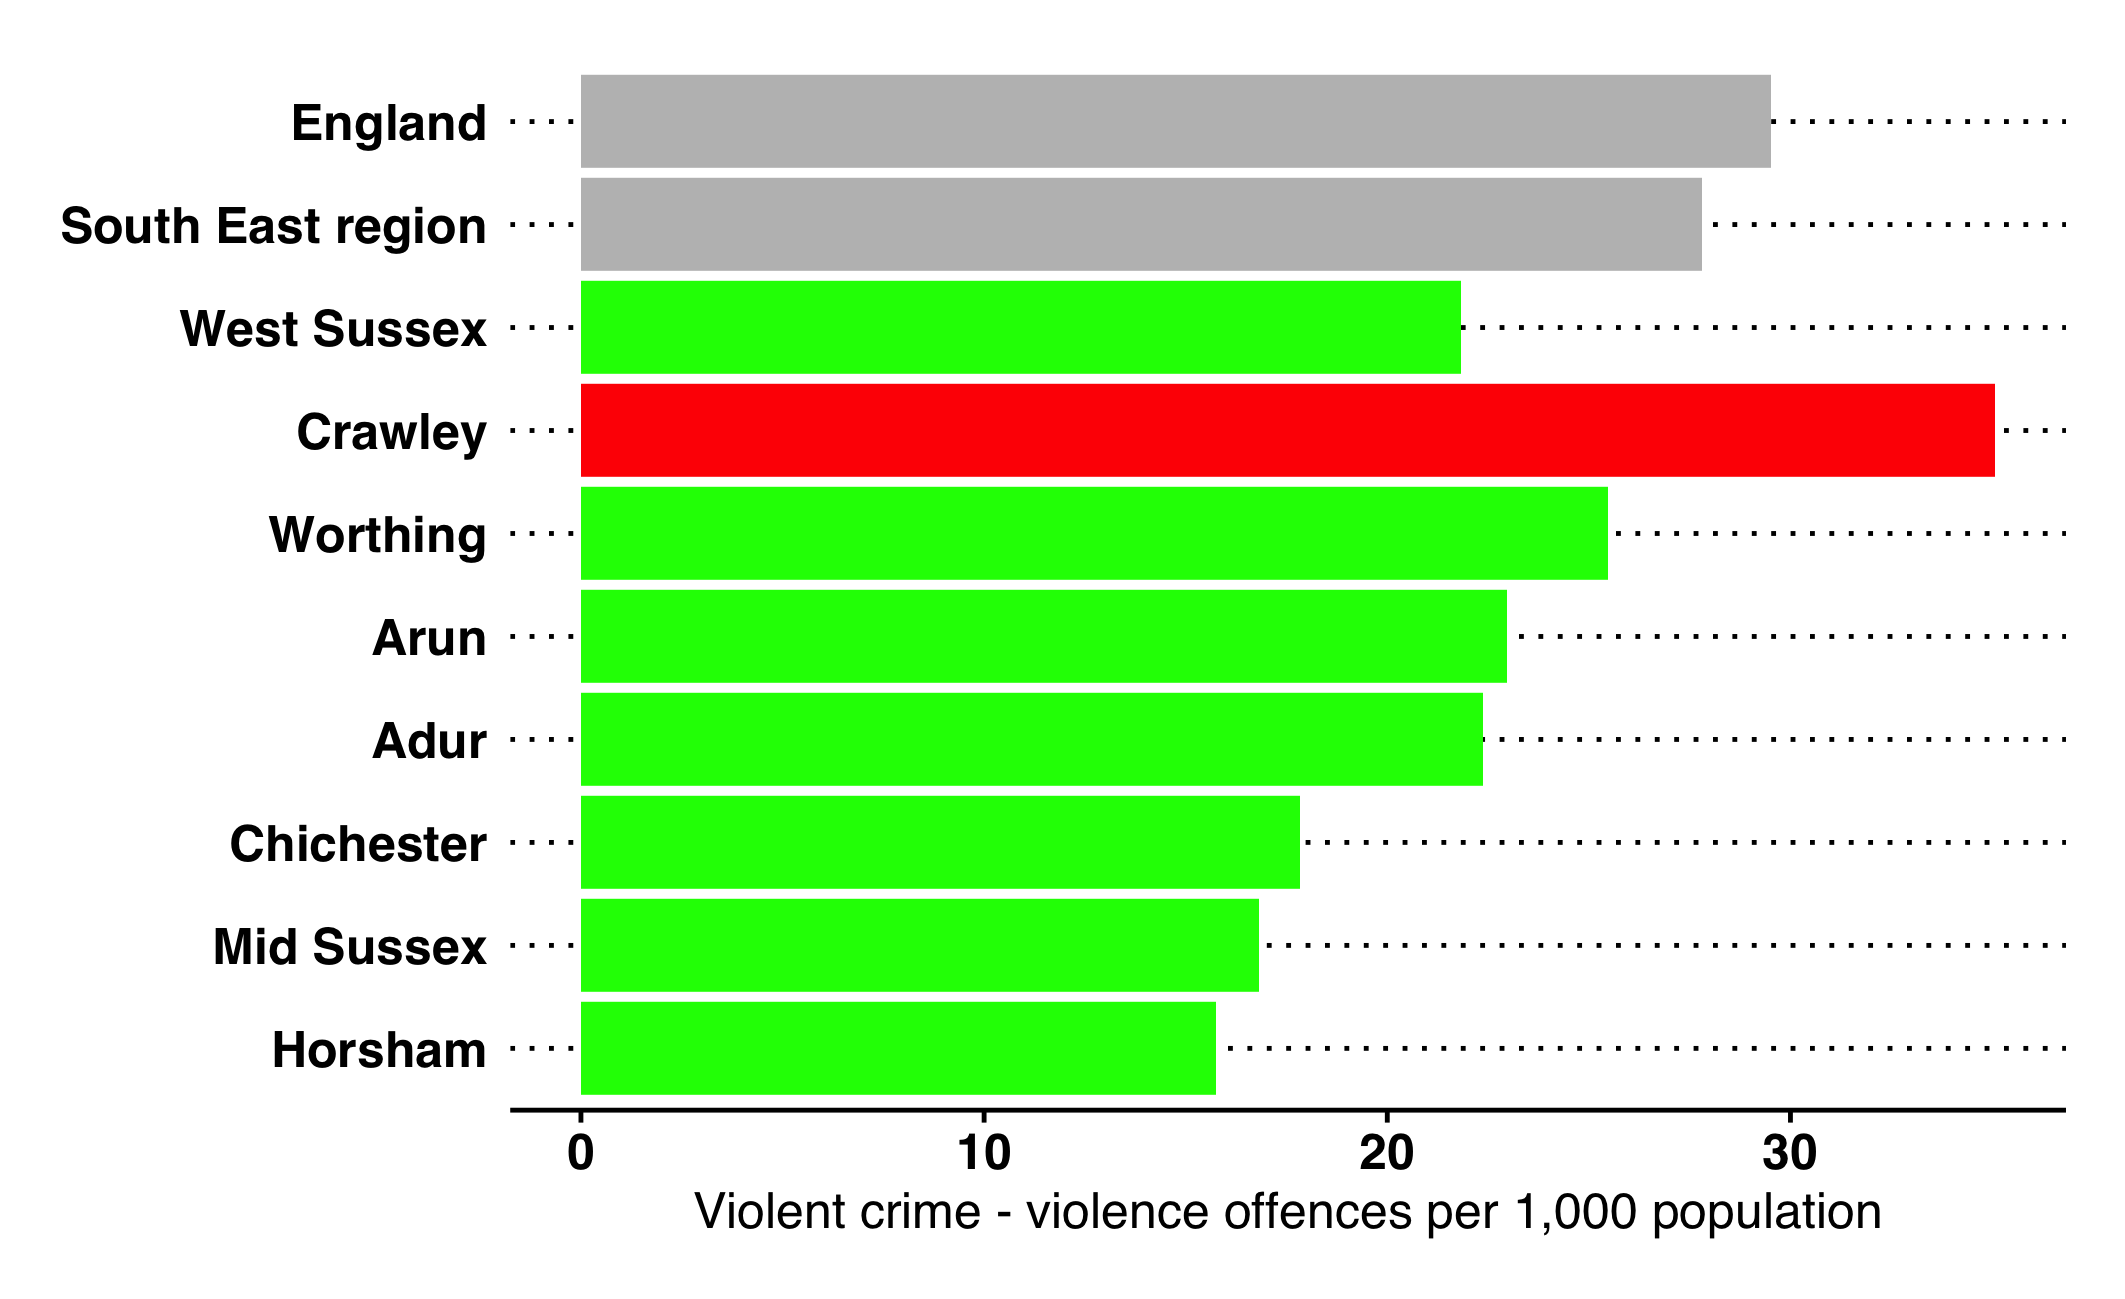
\includegraphics[width=\linewidth]{images/violent_offences_bar.png}
%     \label{fig:suicidviolence:ltla}
% \end{figure}

% FIGURE - LTLA Rate per 1,000 population

% \begin{figure}[htp]
%     \caption[Violent offences per 1,000 population (all ages) over time]{Violent offences per 1,000 population (all ages) over time compared to England.\footnote{PHOF reference B12b}.}
%     \centering
%     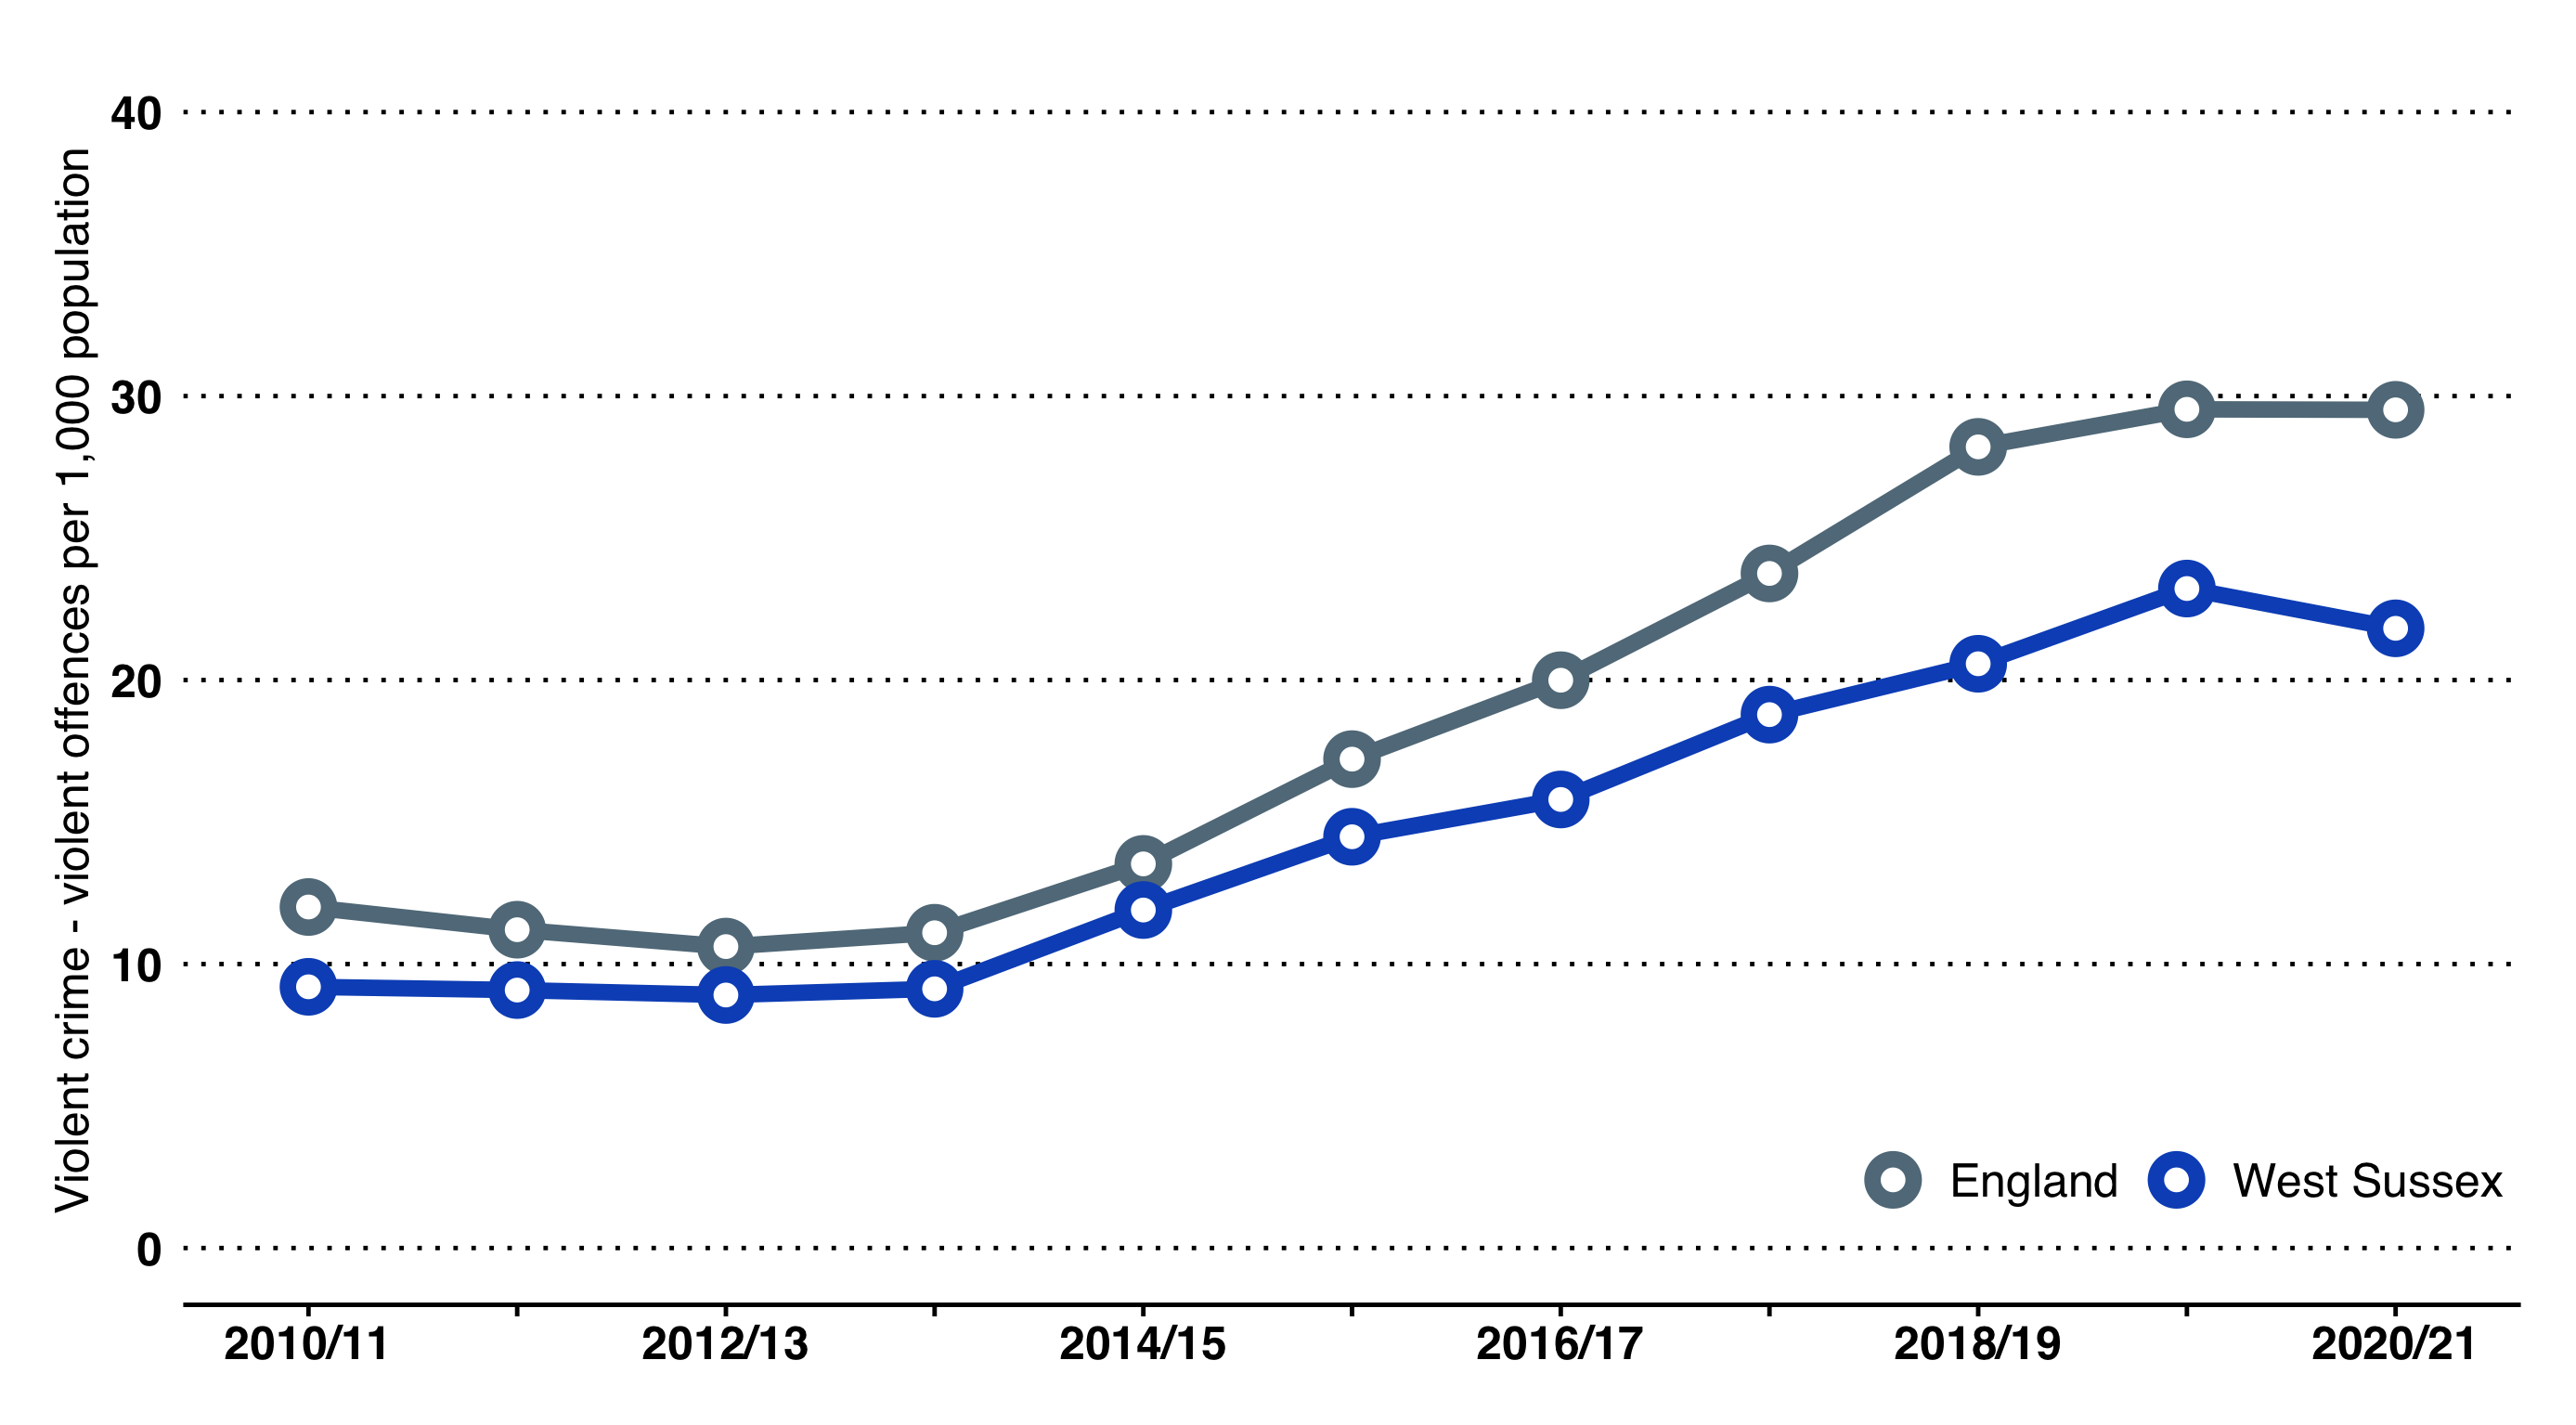
\includegraphics[width=\linewidth]{images/violent_offenses_line.png}
%     \label{fig:violence:time}
% \end{figure}

\subsubsection{Sexual offences} Sexual offences (measured per 1,000 population)\footnote{PHOF reference B12c} have also more than doubled in West Sussex over the last eight years, in line with national rises. In 2020/21, there were 1,602 recorded sexual offences, compared with 697 in 2013/14 (though a decrease on 2019/20).

The rate in West Sussex (1.9 per 1,000 population) remains lower than England (2.3 per 1,000) and is the seventh lowest amongst CIPFA neighbours. Crawley exceeds the national and West Sussex rates, at 2.8 per 1,000.

% FIGURE - Rate per 1,000 population over time (West Sussex vs South East vs England)

% \begin{figure}[htp]
%     \caption[Sexual offences per 1,000 population (all ages) over time]{Sexual offences per 1,000 population (all ages) over time compared to England.\footnote{PHOF reference B12c}.}
%     \centering
%     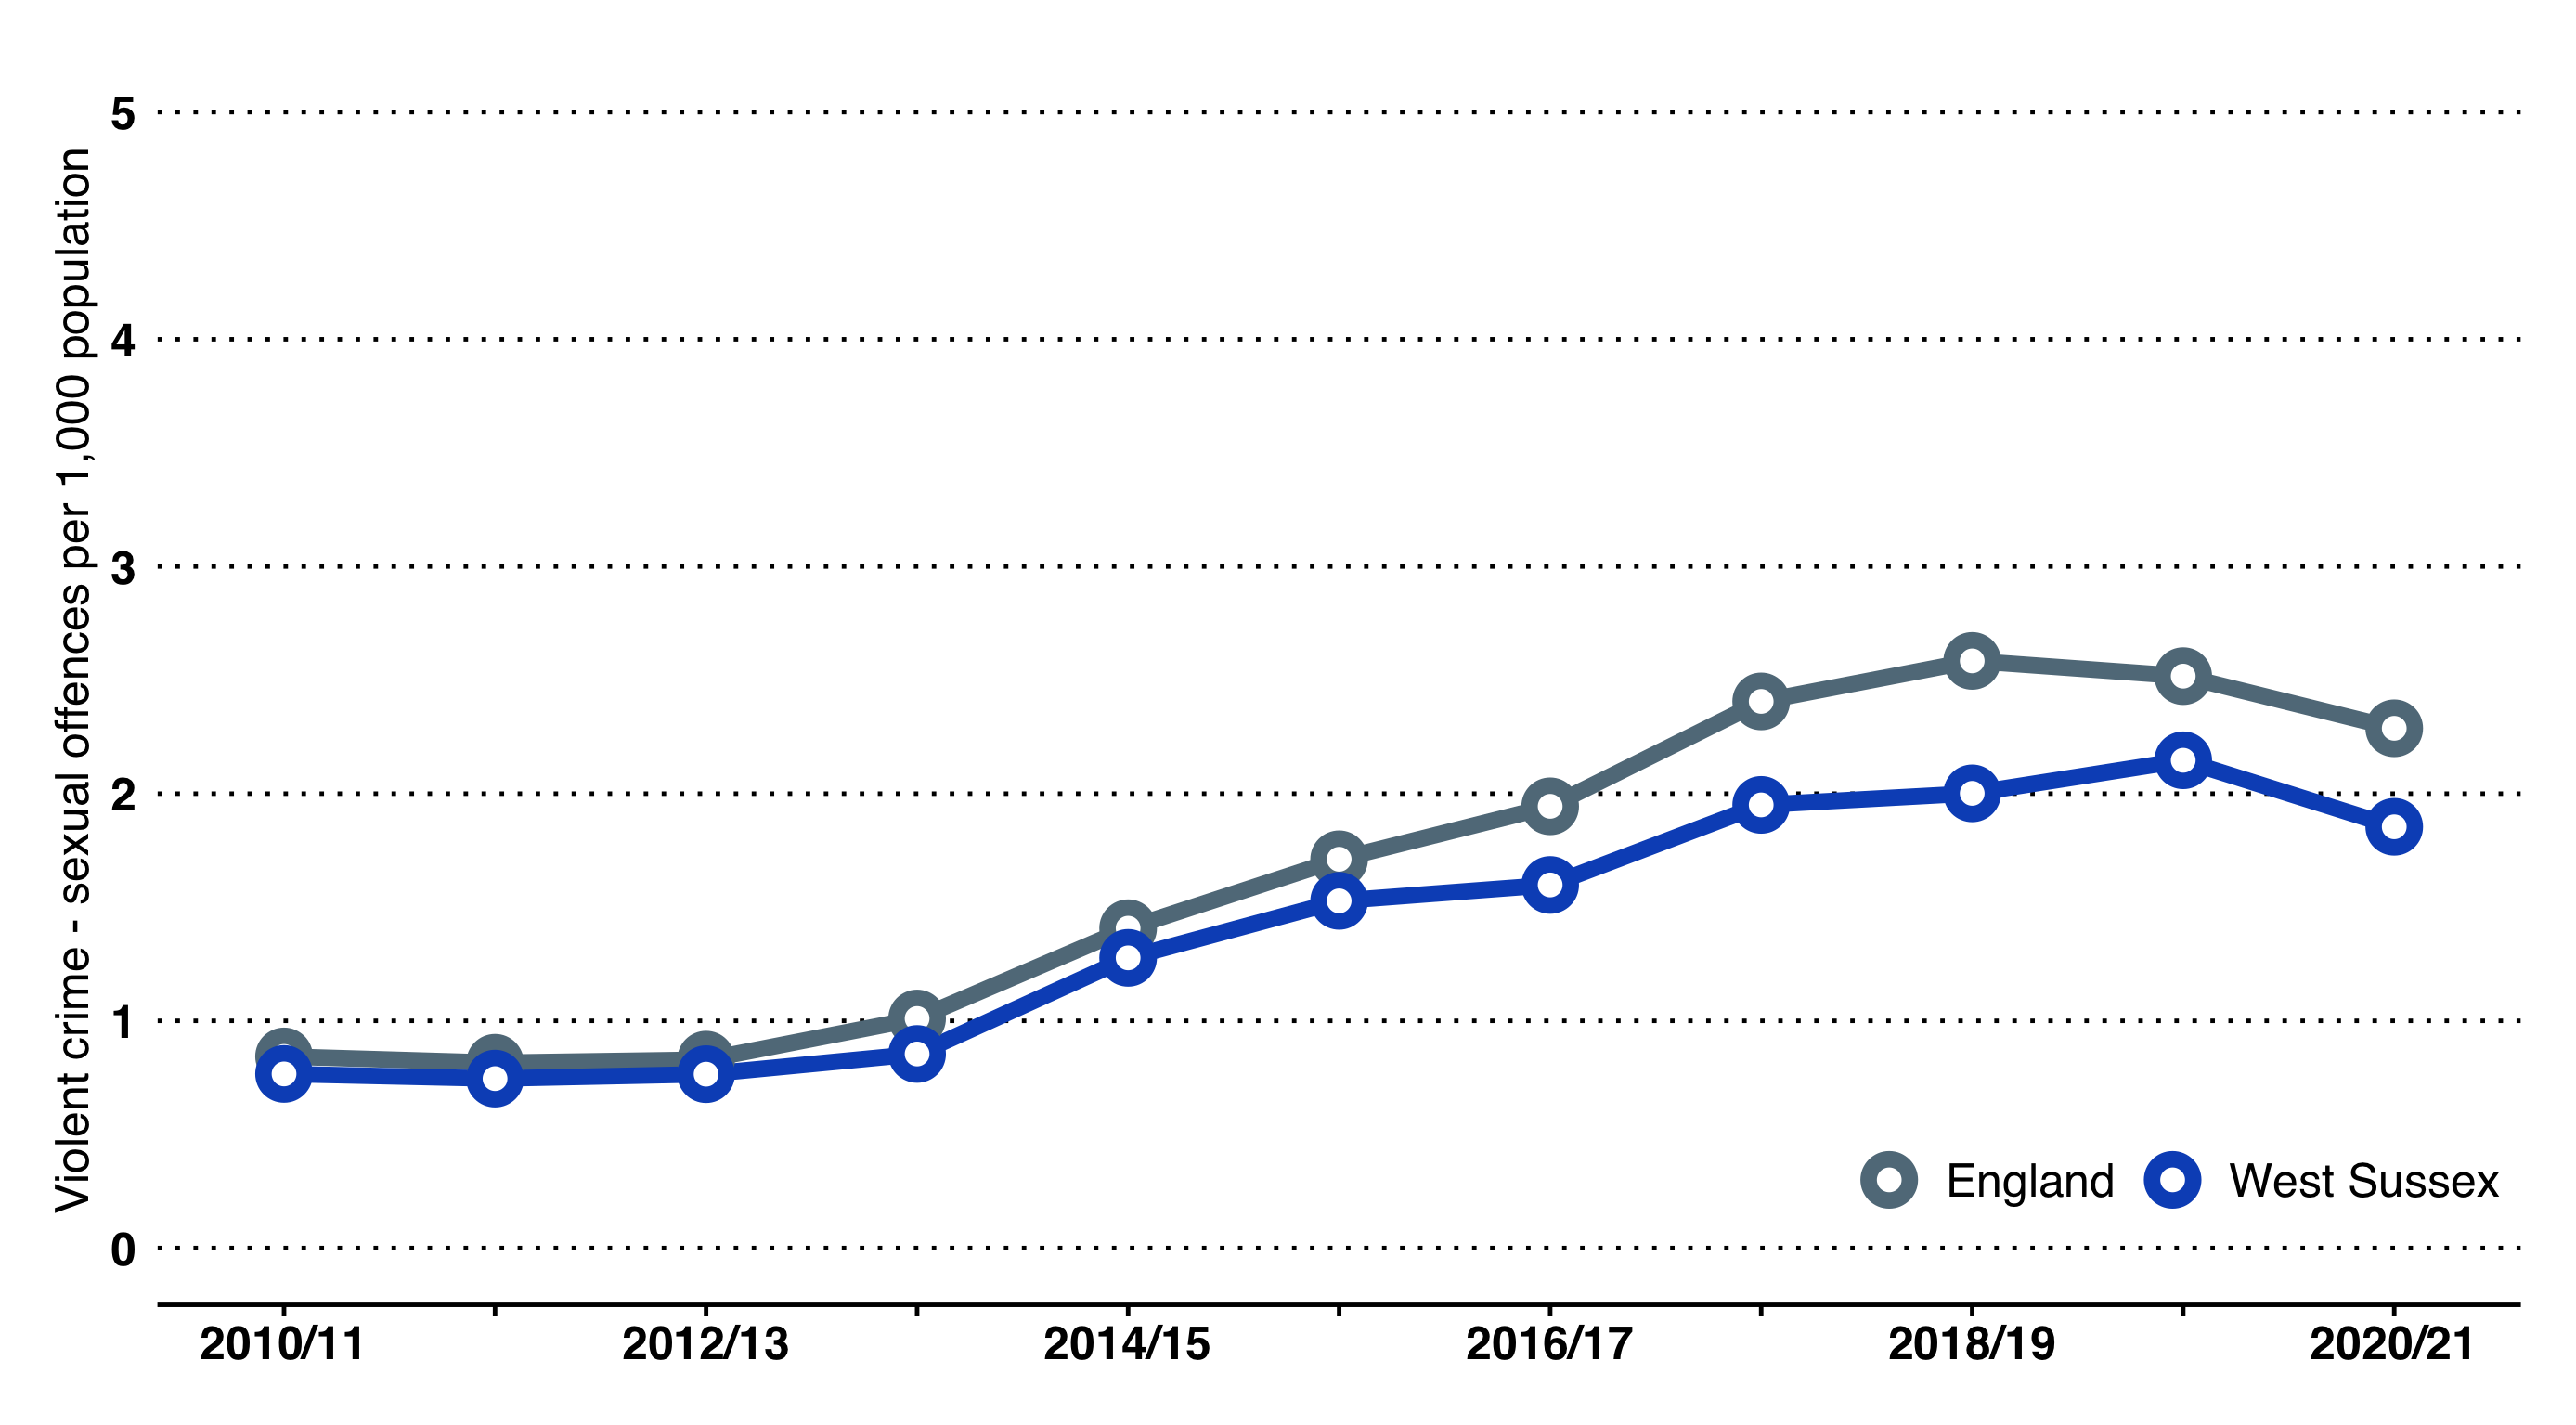
\includegraphics[width=\linewidth]{images/sexual_offences_line.png}
%     \label{fig:sexual_off:time}
% \end{figure}

\subsubsection{Domestic abuse} In 2020/21, the rate of domestic abuse-related incidents and crime\footnote{PHOF reference B11. Note that local authorities are allocated the rate of the police force within which they sit.} was 22.1 per 1,000 in West Sussex, significantly below the national rate of 30.3 per 1,000 and one of the lowest amongst CIPFA neighbours.

\subsubsection{Road accidents} Whilst the national number of people killed or seriously injured (KSI) on roads\footnote{PHOF reference B10.} has remained stable in recent years, there has been an upward trend in West Sussex. At 131.0 per billion vehice miles (equal to 576 people in 2019 and 505 people in 2020), West Sussex has one of the highest KSI rates in the country (England 86.1 per billion vehicle miles). Note that Figure~\ref{fig:ksi:dabs} refers to historic data, as no information are available for districts and boroughs post-2020.

% \begin{figure}[htp]
%     \caption[number of people killed or seriously injured (KSI) on roads per 1,000 population (all ages) over time]{Number of people killed or seriously injured (KSI) on roads per 1,000 population (all ages) in West Sussex districts and boroughs, compared to England.\footnote{PHOF reference B10}.}
%     \centering
%     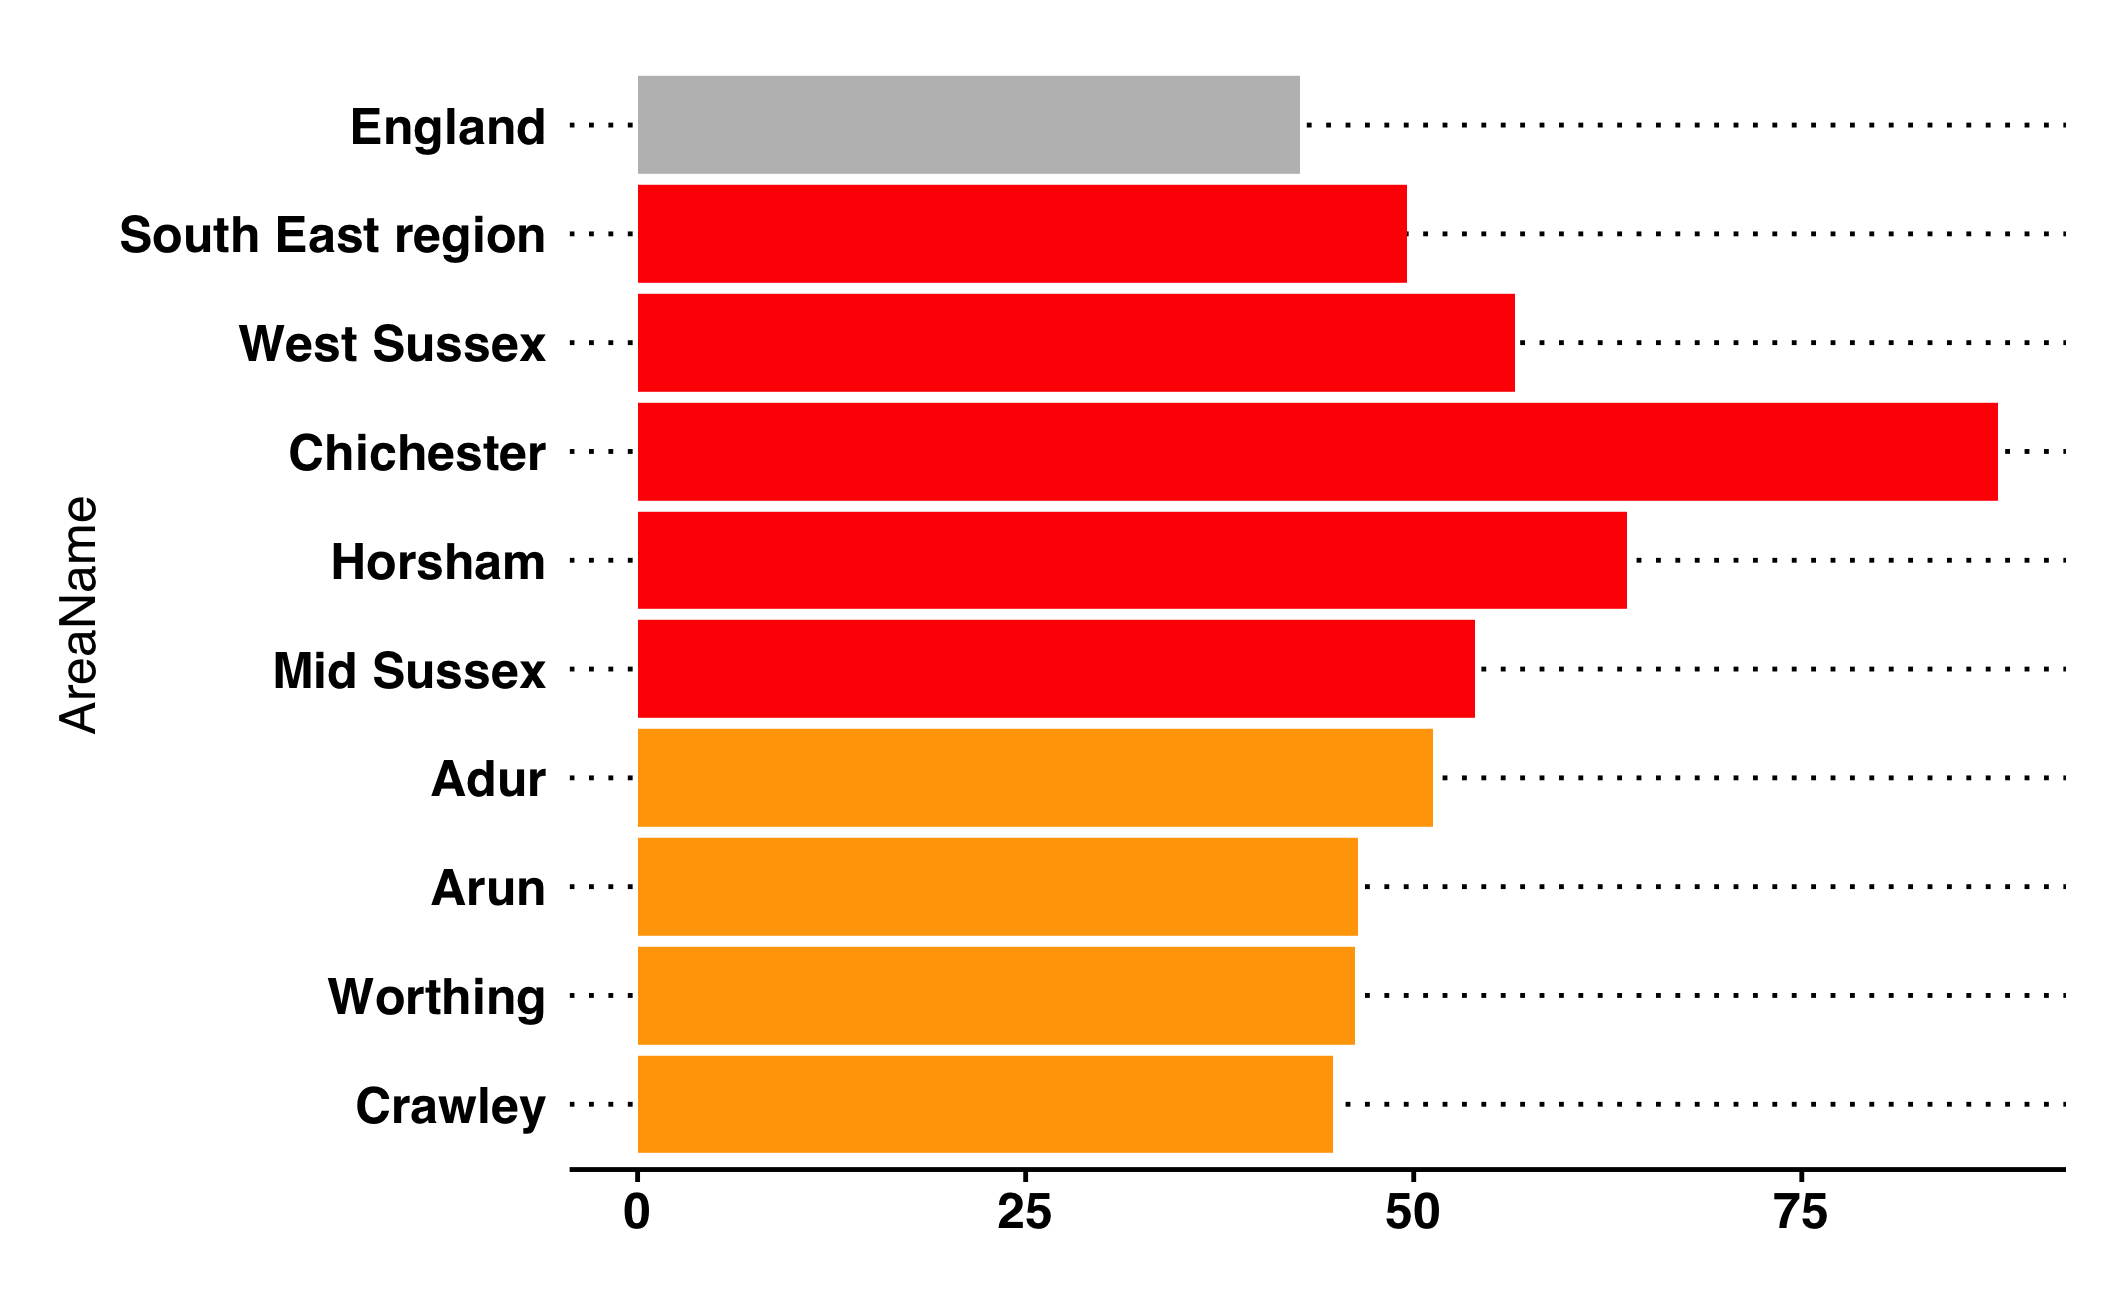
\includegraphics[width=\linewidth]{images/road_accidents_rag.png}
%     \label{fig:ksi:rag}
% \end{figure}

\begin{figure*}
    \caption[Community safety indicators in West Sussex.]{Community safety indicators in West Sussex.}\label{fig:com-safety-inds}
    \vspace*{3mm}
    \centering
    \begin{subfigure}[t]{0.45\textwidth}
        \caption{Number of people killed or seriously injured (KSI) on roads in West Sussex districts and boroughs, compared to England (PHOF reference B10).}\label{fig:ksi:dabs}
        \centering
        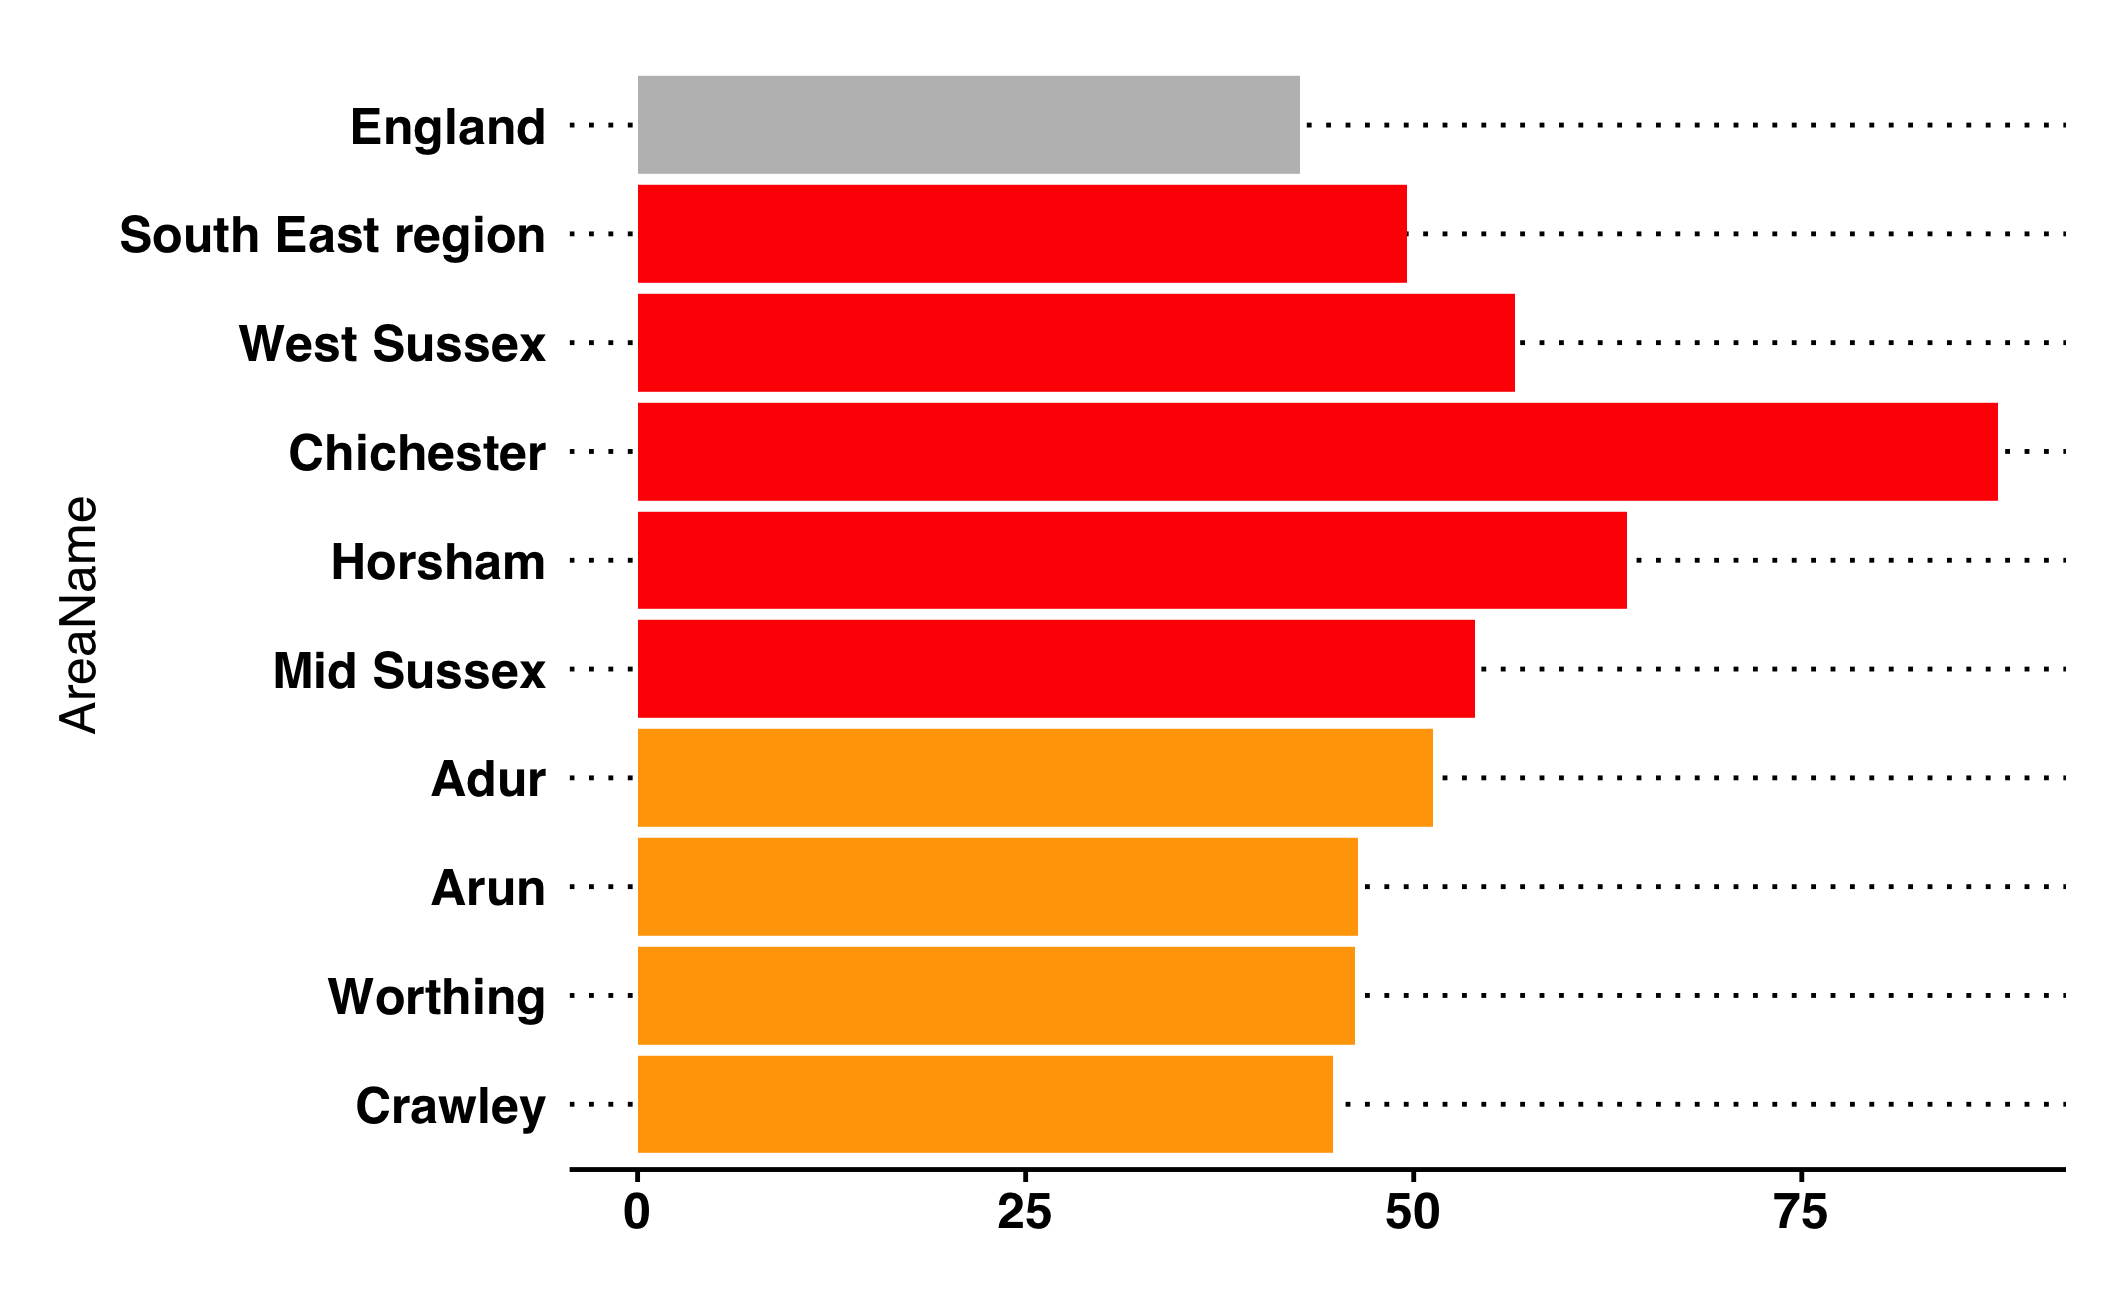
\includegraphics[width=.7\textwidth]{images/road_accidents_rag.png}
    \end{subfigure}
    \begin{subfigure}[t]{0.45\textwidth}
        \caption[Violent offences per 1,000 population (all ages) in West Sussex districts and boroughs.]{Violent offences per 1,000 population (all ages) in West Sussex districts and boroughs (PHOF reference B12b).}\label{fig:violence:ltla}
        \centering
        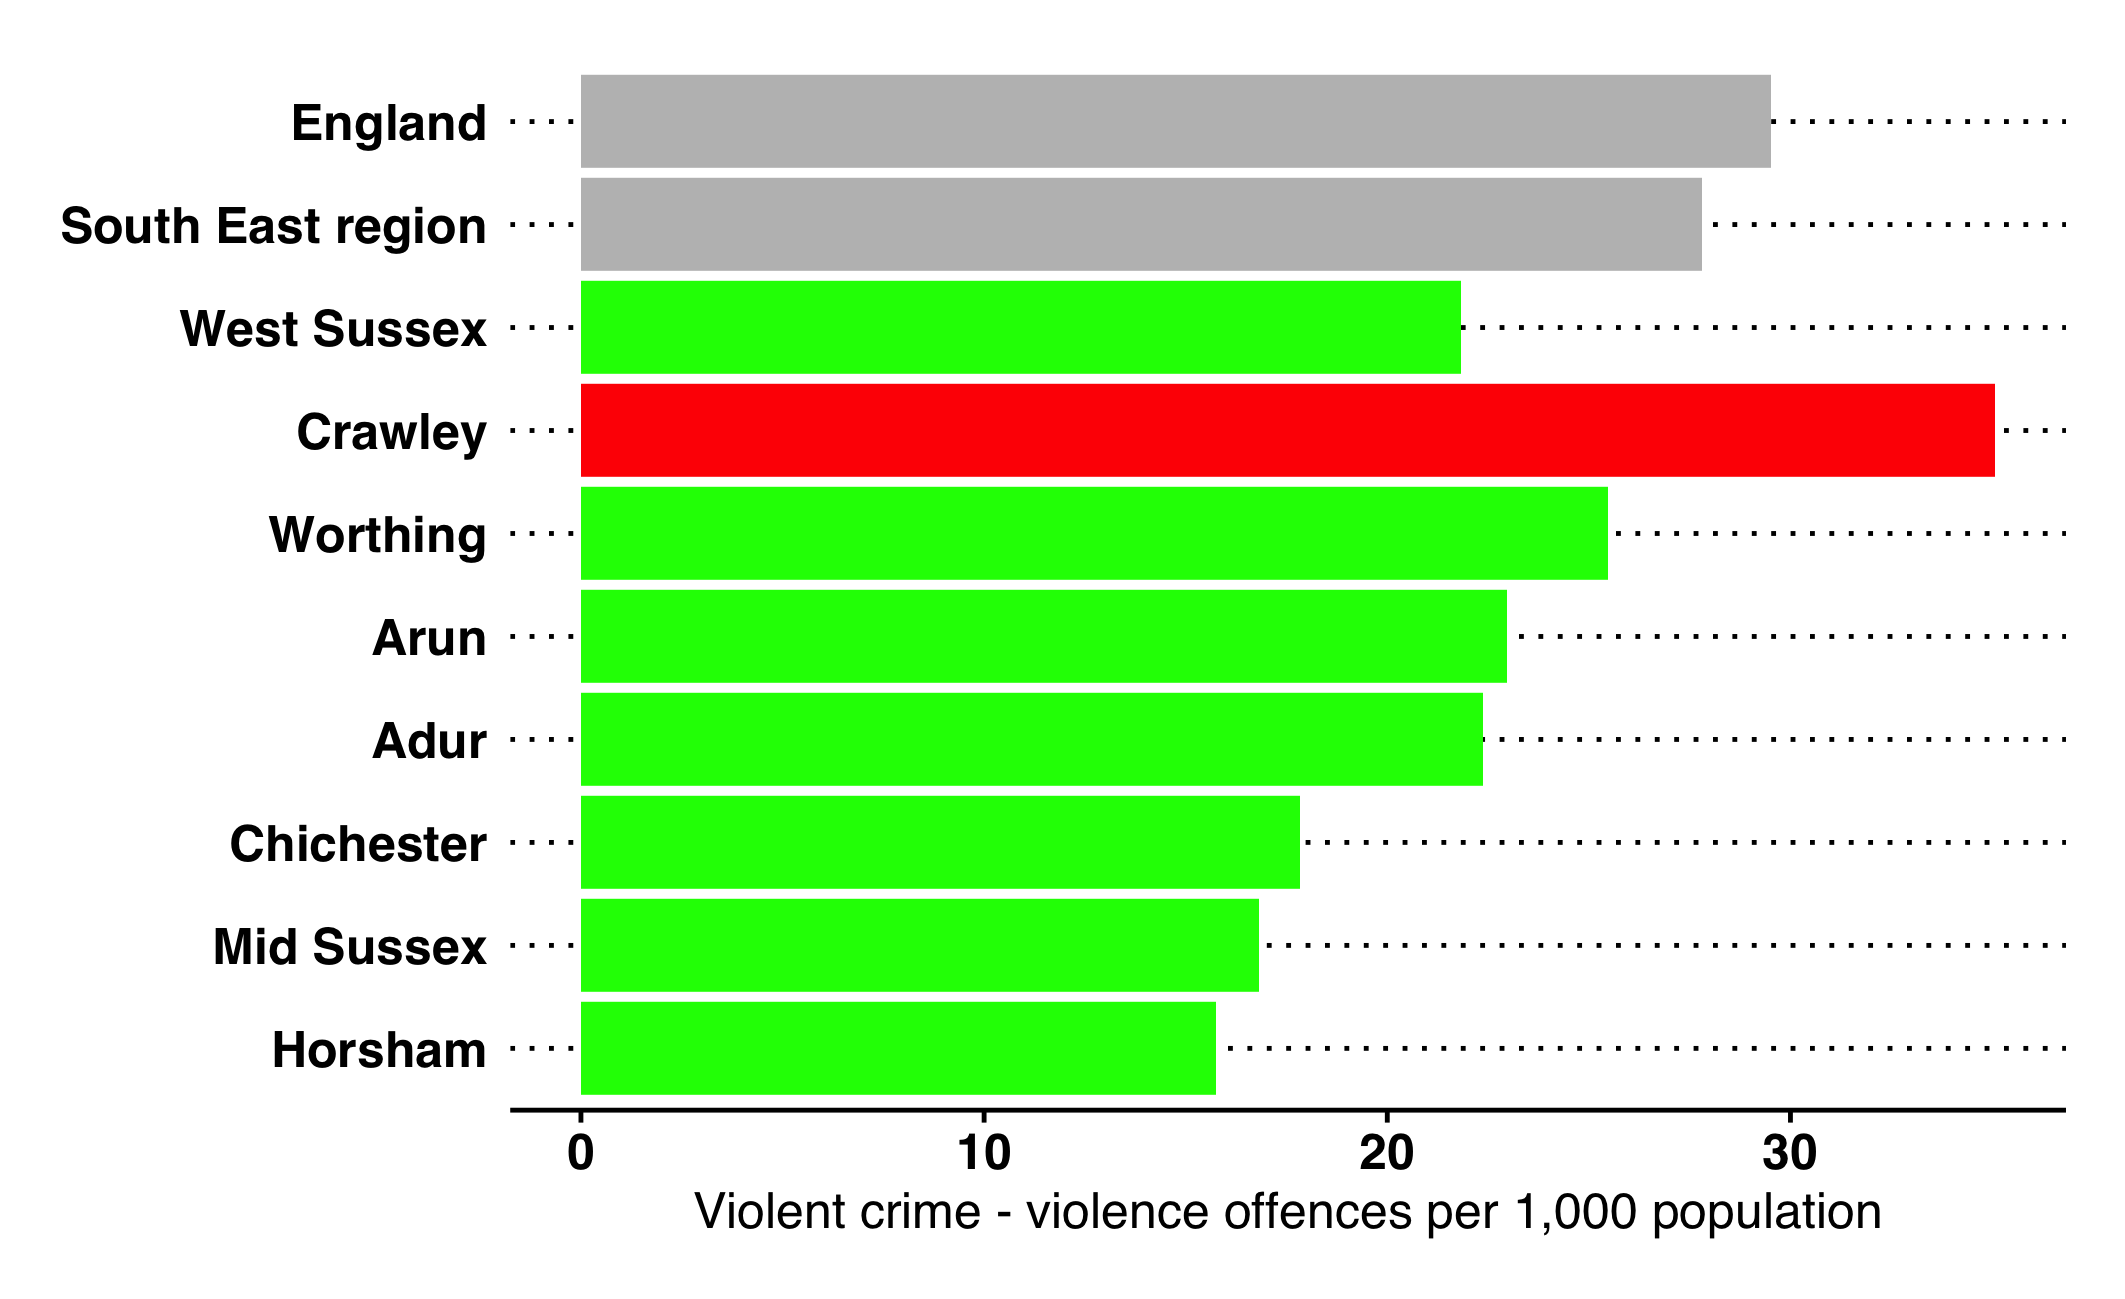
\includegraphics[width=.7\textwidth]{images/violent_offences_bar.png}
    \end{subfigure}
    \begin{subfigure}[t]{0.45\textwidth}
        \caption[Violent offences per 1,000 population (all ages) over time]{Violent offences per 1,000 population (all ages) over time compared to England (PHOF reference B12b).}\label{fig:violence:time}
        \centering
        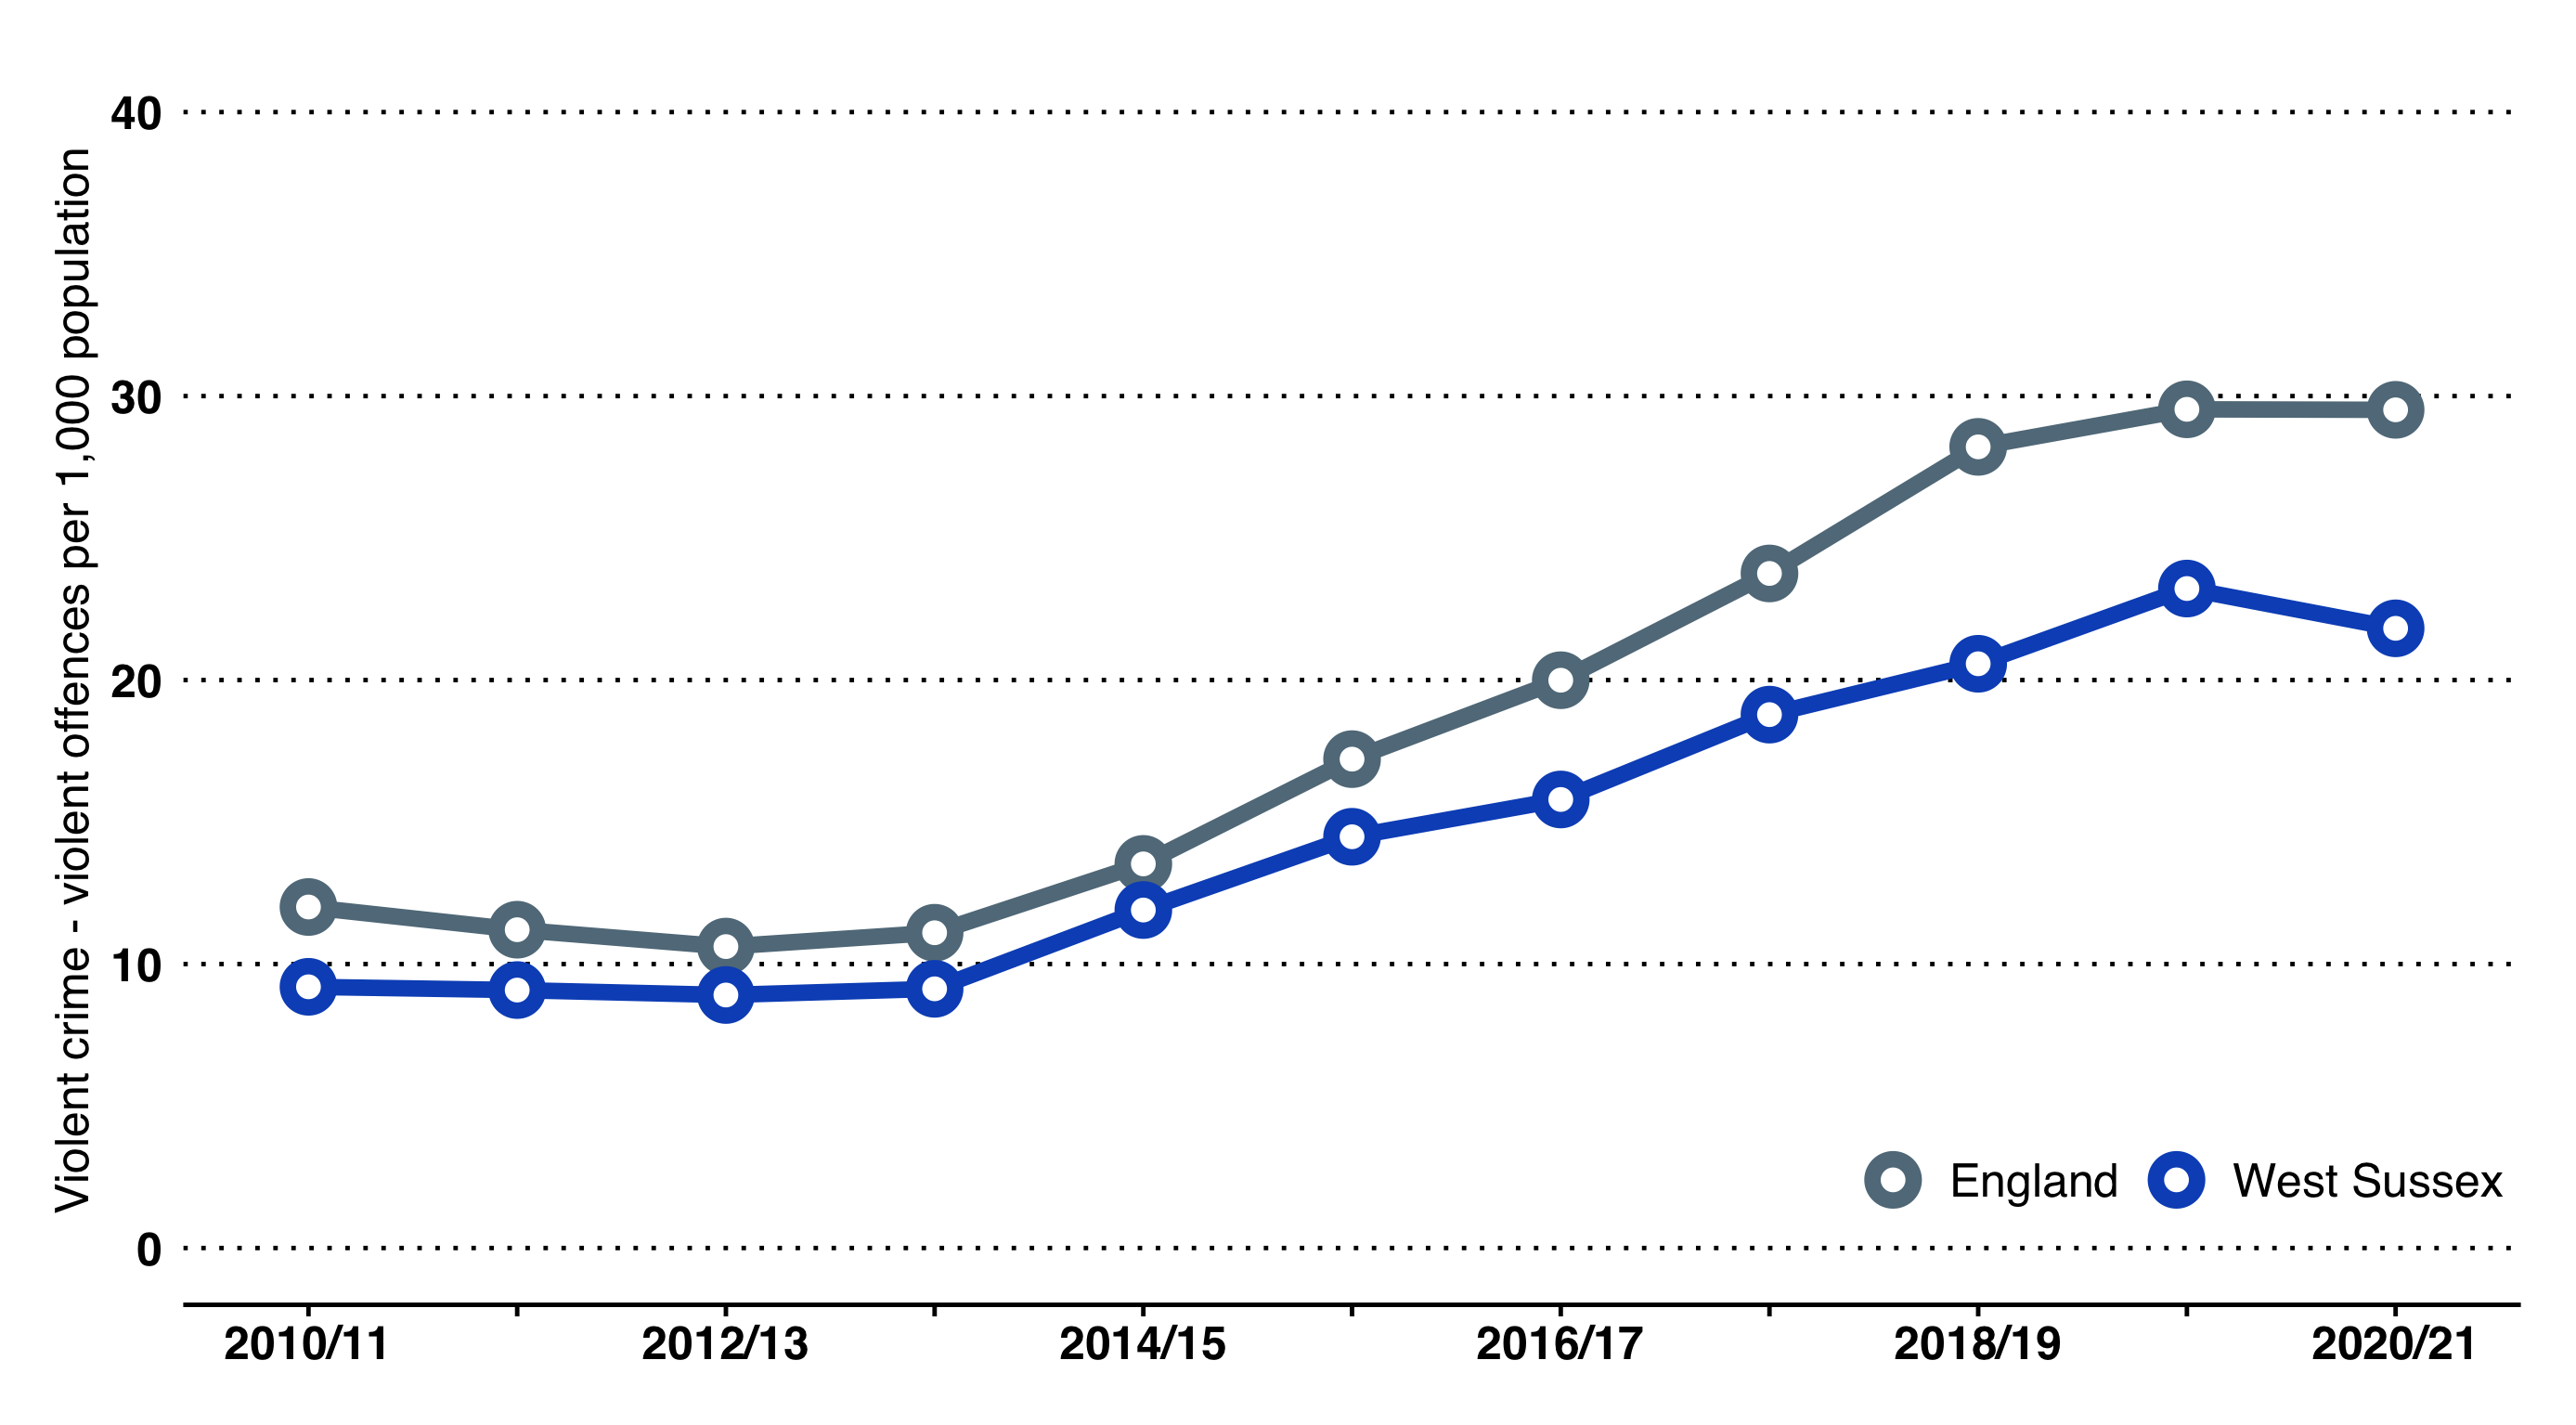
\includegraphics[width=\textwidth]{images/violent_offenses_line.png}
    \end{subfigure}
    \begin{subfigure}[t]{0.45\textwidth}
        \caption[Sexual offences per 1,000 population (all ages) over time]{Sexual offences per 1,000 population (all ages) over time compared to England (PHOF reference B12c).}\label{fig:sexual_off:time}
        \centering
        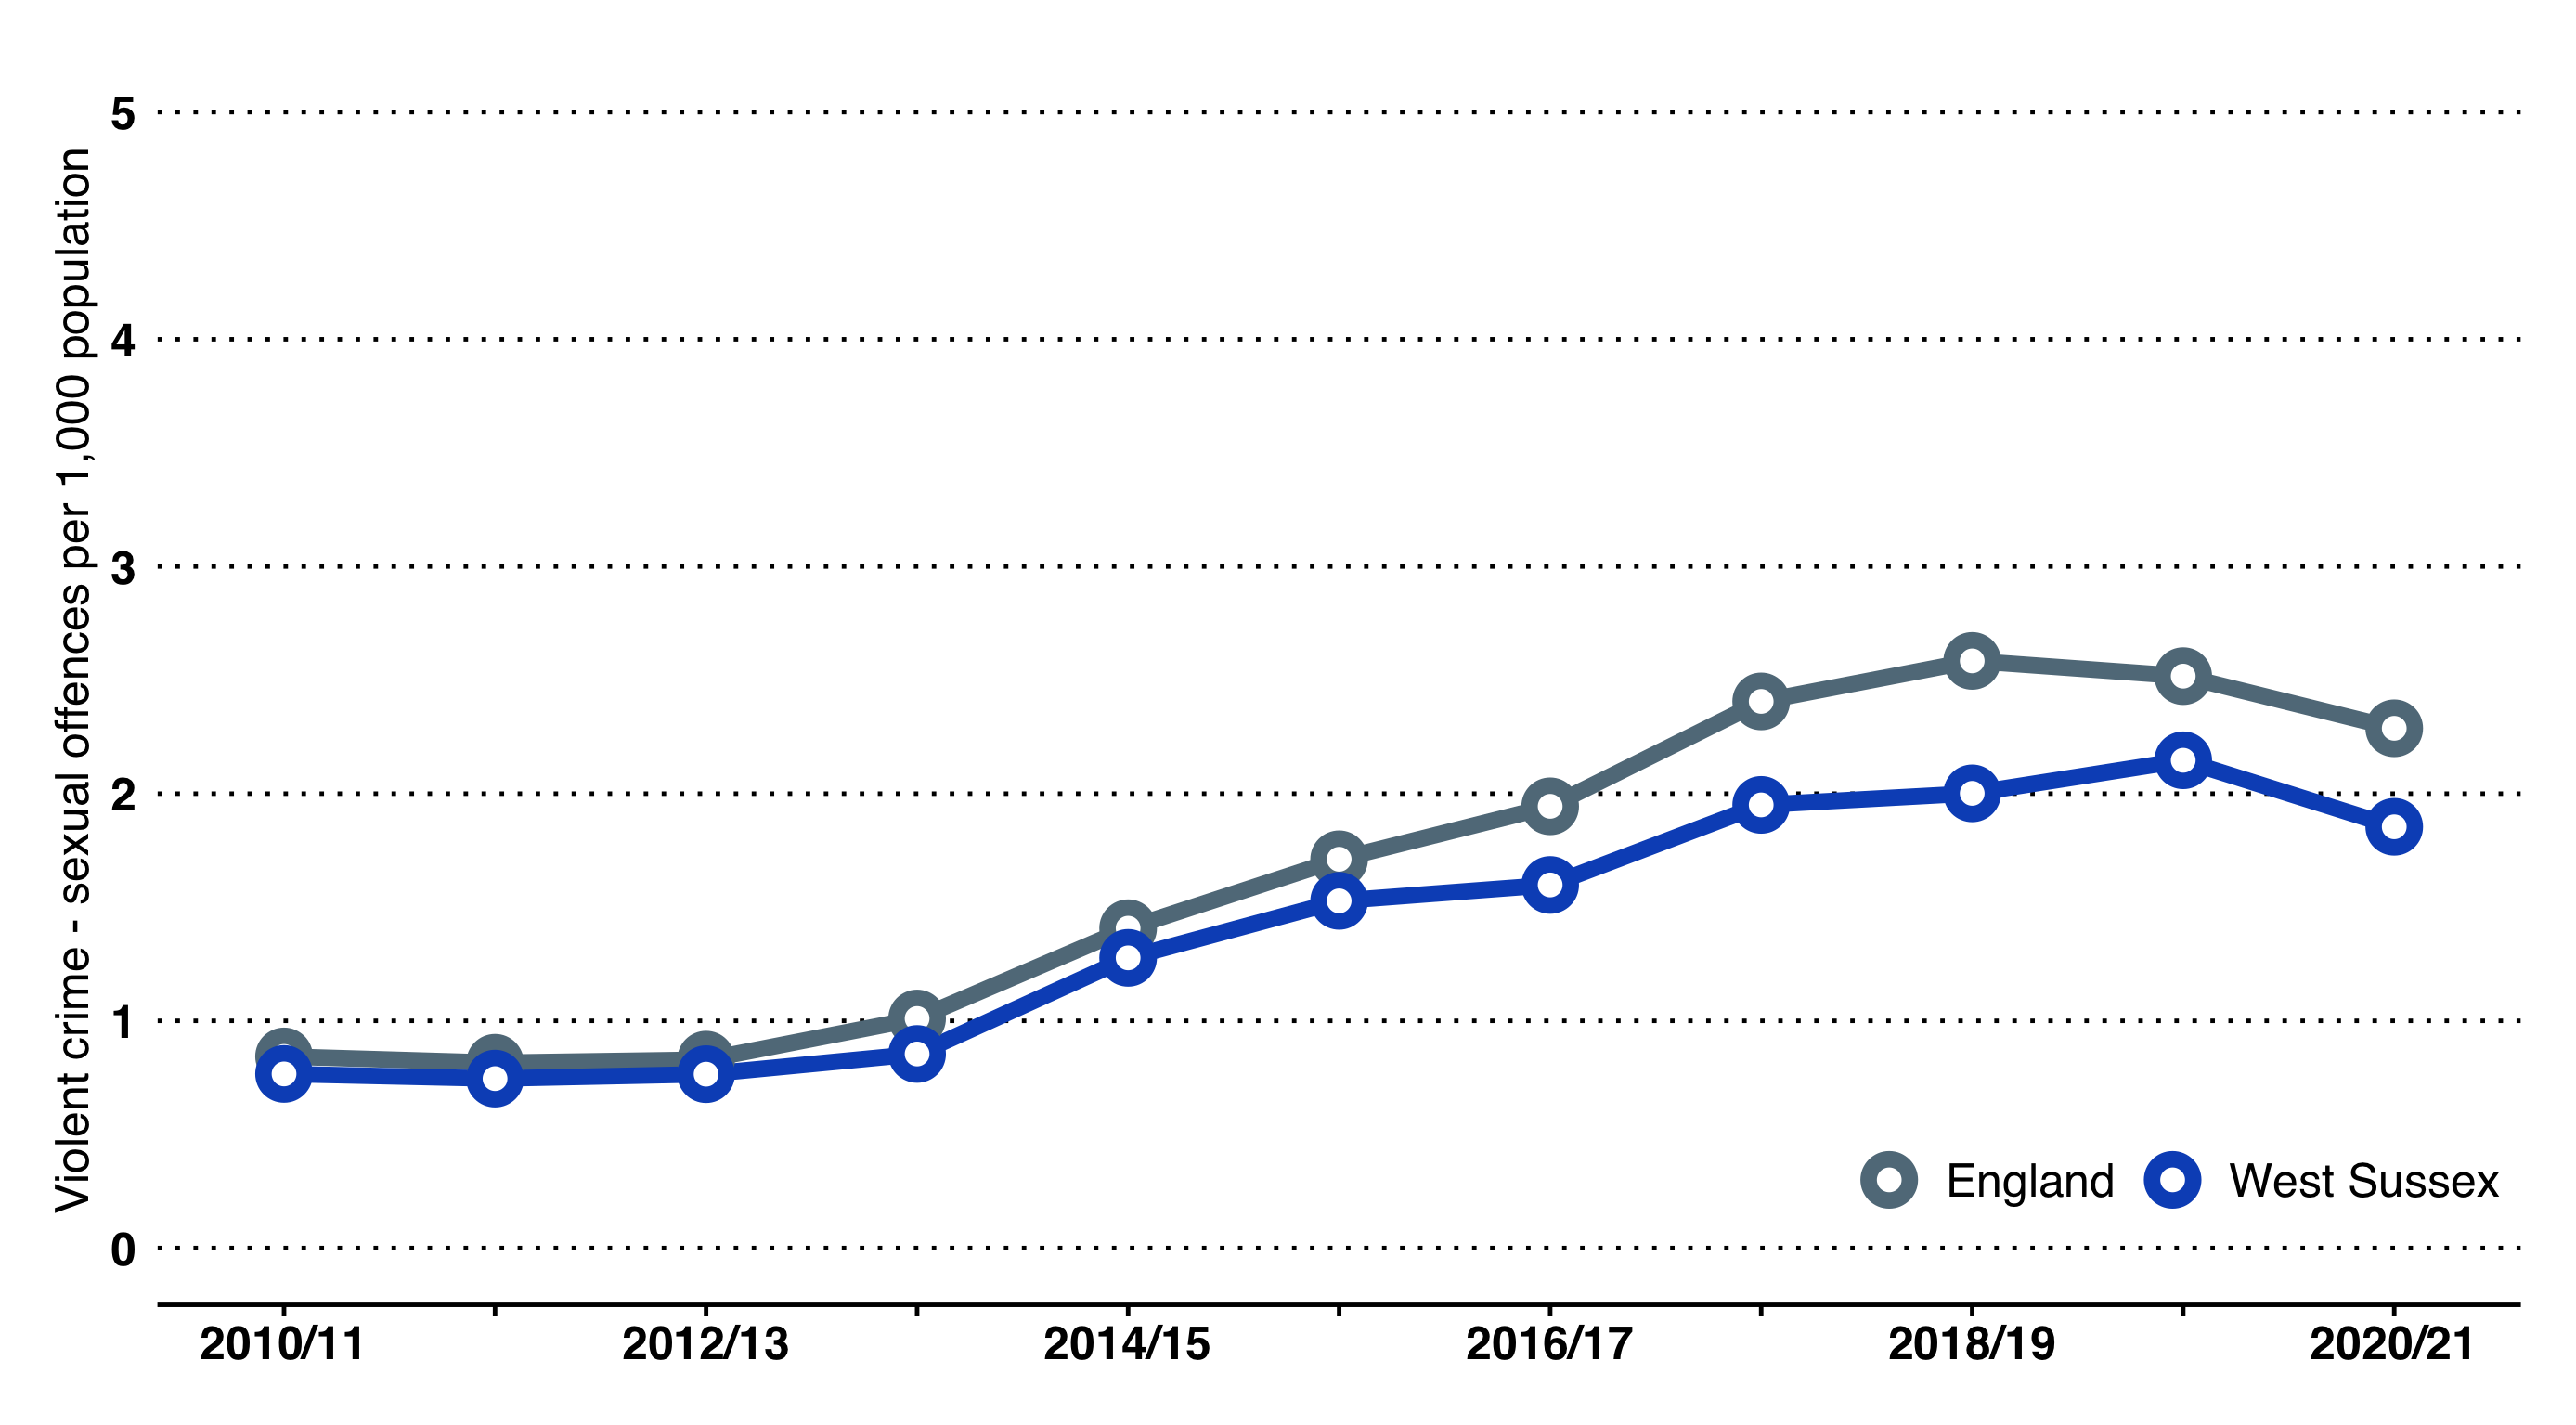
\includegraphics[width=\textwidth]{images/sexual_offences_line.png}
    \end{subfigure}
\end{figure*}

% FIGURE - LTLA Rate per 100,000 population


% \subsection{Further information}

% This is a summary document; more detailed local analyses (alongside a whole host of national profiles!) are available, including the needs assessment and briefings highlighted below. If you have specific information requests please contact the team.

% In addition to the contacts shown in the summary, overall for overall queries for Living Well in the West Sussex Public Health and Social Research Team contact Jacqueline Clay - (\url{jacqueline.clay@westsussex.gov.uk})